% Options for packages loaded elsewhere
\PassOptionsToPackage{unicode}{hyperref}
\PassOptionsToPackage{hyphens}{url}
\PassOptionsToPackage{dvipsnames,svgnames,x11names}{xcolor}
%
\documentclass[
  letterpaper,
  DIV=11,
  numbers=noendperiod]{scrreprt}

\usepackage{amsmath,amssymb}
\usepackage{iftex}
\ifPDFTeX
  \usepackage[T1]{fontenc}
  \usepackage[utf8]{inputenc}
  \usepackage{textcomp} % provide euro and other symbols
\else % if luatex or xetex
  \usepackage{unicode-math}
  \defaultfontfeatures{Scale=MatchLowercase}
  \defaultfontfeatures[\rmfamily]{Ligatures=TeX,Scale=1}
\fi
\usepackage{lmodern}
\ifPDFTeX\else  
    % xetex/luatex font selection
\fi
% Use upquote if available, for straight quotes in verbatim environments
\IfFileExists{upquote.sty}{\usepackage{upquote}}{}
\IfFileExists{microtype.sty}{% use microtype if available
  \usepackage[]{microtype}
  \UseMicrotypeSet[protrusion]{basicmath} % disable protrusion for tt fonts
}{}
\makeatletter
\@ifundefined{KOMAClassName}{% if non-KOMA class
  \IfFileExists{parskip.sty}{%
    \usepackage{parskip}
  }{% else
    \setlength{\parindent}{0pt}
    \setlength{\parskip}{6pt plus 2pt minus 1pt}}
}{% if KOMA class
  \KOMAoptions{parskip=half}}
\makeatother
\usepackage{xcolor}
\setlength{\emergencystretch}{3em} % prevent overfull lines
\setcounter{secnumdepth}{5}
% Make \paragraph and \subparagraph free-standing
\makeatletter
\ifx\paragraph\undefined\else
  \let\oldparagraph\paragraph
  \renewcommand{\paragraph}{
    \@ifstar
      \xxxParagraphStar
      \xxxParagraphNoStar
  }
  \newcommand{\xxxParagraphStar}[1]{\oldparagraph*{#1}\mbox{}}
  \newcommand{\xxxParagraphNoStar}[1]{\oldparagraph{#1}\mbox{}}
\fi
\ifx\subparagraph\undefined\else
  \let\oldsubparagraph\subparagraph
  \renewcommand{\subparagraph}{
    \@ifstar
      \xxxSubParagraphStar
      \xxxSubParagraphNoStar
  }
  \newcommand{\xxxSubParagraphStar}[1]{\oldsubparagraph*{#1}\mbox{}}
  \newcommand{\xxxSubParagraphNoStar}[1]{\oldsubparagraph{#1}\mbox{}}
\fi
\makeatother

\usepackage{color}
\usepackage{fancyvrb}
\newcommand{\VerbBar}{|}
\newcommand{\VERB}{\Verb[commandchars=\\\{\}]}
\DefineVerbatimEnvironment{Highlighting}{Verbatim}{commandchars=\\\{\}}
% Add ',fontsize=\small' for more characters per line
\usepackage{framed}
\definecolor{shadecolor}{RGB}{241,243,245}
\newenvironment{Shaded}{\begin{snugshade}}{\end{snugshade}}
\newcommand{\AlertTok}[1]{\textcolor[rgb]{0.68,0.00,0.00}{#1}}
\newcommand{\AnnotationTok}[1]{\textcolor[rgb]{0.37,0.37,0.37}{#1}}
\newcommand{\AttributeTok}[1]{\textcolor[rgb]{0.40,0.45,0.13}{#1}}
\newcommand{\BaseNTok}[1]{\textcolor[rgb]{0.68,0.00,0.00}{#1}}
\newcommand{\BuiltInTok}[1]{\textcolor[rgb]{0.00,0.23,0.31}{#1}}
\newcommand{\CharTok}[1]{\textcolor[rgb]{0.13,0.47,0.30}{#1}}
\newcommand{\CommentTok}[1]{\textcolor[rgb]{0.37,0.37,0.37}{#1}}
\newcommand{\CommentVarTok}[1]{\textcolor[rgb]{0.37,0.37,0.37}{\textit{#1}}}
\newcommand{\ConstantTok}[1]{\textcolor[rgb]{0.56,0.35,0.01}{#1}}
\newcommand{\ControlFlowTok}[1]{\textcolor[rgb]{0.00,0.23,0.31}{\textbf{#1}}}
\newcommand{\DataTypeTok}[1]{\textcolor[rgb]{0.68,0.00,0.00}{#1}}
\newcommand{\DecValTok}[1]{\textcolor[rgb]{0.68,0.00,0.00}{#1}}
\newcommand{\DocumentationTok}[1]{\textcolor[rgb]{0.37,0.37,0.37}{\textit{#1}}}
\newcommand{\ErrorTok}[1]{\textcolor[rgb]{0.68,0.00,0.00}{#1}}
\newcommand{\ExtensionTok}[1]{\textcolor[rgb]{0.00,0.23,0.31}{#1}}
\newcommand{\FloatTok}[1]{\textcolor[rgb]{0.68,0.00,0.00}{#1}}
\newcommand{\FunctionTok}[1]{\textcolor[rgb]{0.28,0.35,0.67}{#1}}
\newcommand{\ImportTok}[1]{\textcolor[rgb]{0.00,0.46,0.62}{#1}}
\newcommand{\InformationTok}[1]{\textcolor[rgb]{0.37,0.37,0.37}{#1}}
\newcommand{\KeywordTok}[1]{\textcolor[rgb]{0.00,0.23,0.31}{\textbf{#1}}}
\newcommand{\NormalTok}[1]{\textcolor[rgb]{0.00,0.23,0.31}{#1}}
\newcommand{\OperatorTok}[1]{\textcolor[rgb]{0.37,0.37,0.37}{#1}}
\newcommand{\OtherTok}[1]{\textcolor[rgb]{0.00,0.23,0.31}{#1}}
\newcommand{\PreprocessorTok}[1]{\textcolor[rgb]{0.68,0.00,0.00}{#1}}
\newcommand{\RegionMarkerTok}[1]{\textcolor[rgb]{0.00,0.23,0.31}{#1}}
\newcommand{\SpecialCharTok}[1]{\textcolor[rgb]{0.37,0.37,0.37}{#1}}
\newcommand{\SpecialStringTok}[1]{\textcolor[rgb]{0.13,0.47,0.30}{#1}}
\newcommand{\StringTok}[1]{\textcolor[rgb]{0.13,0.47,0.30}{#1}}
\newcommand{\VariableTok}[1]{\textcolor[rgb]{0.07,0.07,0.07}{#1}}
\newcommand{\VerbatimStringTok}[1]{\textcolor[rgb]{0.13,0.47,0.30}{#1}}
\newcommand{\WarningTok}[1]{\textcolor[rgb]{0.37,0.37,0.37}{\textit{#1}}}

\providecommand{\tightlist}{%
  \setlength{\itemsep}{0pt}\setlength{\parskip}{0pt}}\usepackage{longtable,booktabs,array}
\usepackage{calc} % for calculating minipage widths
% Correct order of tables after \paragraph or \subparagraph
\usepackage{etoolbox}
\makeatletter
\patchcmd\longtable{\par}{\if@noskipsec\mbox{}\fi\par}{}{}
\makeatother
% Allow footnotes in longtable head/foot
\IfFileExists{footnotehyper.sty}{\usepackage{footnotehyper}}{\usepackage{footnote}}
\makesavenoteenv{longtable}
\usepackage{graphicx}
\makeatletter
\newsavebox\pandoc@box
\newcommand*\pandocbounded[1]{% scales image to fit in text height/width
  \sbox\pandoc@box{#1}%
  \Gscale@div\@tempa{\textheight}{\dimexpr\ht\pandoc@box+\dp\pandoc@box\relax}%
  \Gscale@div\@tempb{\linewidth}{\wd\pandoc@box}%
  \ifdim\@tempb\p@<\@tempa\p@\let\@tempa\@tempb\fi% select the smaller of both
  \ifdim\@tempa\p@<\p@\scalebox{\@tempa}{\usebox\pandoc@box}%
  \else\usebox{\pandoc@box}%
  \fi%
}
% Set default figure placement to htbp
\def\fps@figure{htbp}
\makeatother
% definitions for citeproc citations
\NewDocumentCommand\citeproctext{}{}
\NewDocumentCommand\citeproc{mm}{%
  \begingroup\def\citeproctext{#2}\cite{#1}\endgroup}
\makeatletter
 % allow citations to break across lines
 \let\@cite@ofmt\@firstofone
 % avoid brackets around text for \cite:
 \def\@biblabel#1{}
 \def\@cite#1#2{{#1\if@tempswa , #2\fi}}
\makeatother
\newlength{\cslhangindent}
\setlength{\cslhangindent}{1.5em}
\newlength{\csllabelwidth}
\setlength{\csllabelwidth}{3em}
\newenvironment{CSLReferences}[2] % #1 hanging-indent, #2 entry-spacing
 {\begin{list}{}{%
  \setlength{\itemindent}{0pt}
  \setlength{\leftmargin}{0pt}
  \setlength{\parsep}{0pt}
  % turn on hanging indent if param 1 is 1
  \ifodd #1
   \setlength{\leftmargin}{\cslhangindent}
   \setlength{\itemindent}{-1\cslhangindent}
  \fi
  % set entry spacing
  \setlength{\itemsep}{#2\baselineskip}}}
 {\end{list}}
\usepackage{calc}
\newcommand{\CSLBlock}[1]{\hfill\break\parbox[t]{\linewidth}{\strut\ignorespaces#1\strut}}
\newcommand{\CSLLeftMargin}[1]{\parbox[t]{\csllabelwidth}{\strut#1\strut}}
\newcommand{\CSLRightInline}[1]{\parbox[t]{\linewidth - \csllabelwidth}{\strut#1\strut}}
\newcommand{\CSLIndent}[1]{\hspace{\cslhangindent}#1}

\KOMAoption{captions}{tableheading}
\makeatletter
\@ifpackageloaded{bookmark}{}{\usepackage{bookmark}}
\makeatother
\makeatletter
\@ifpackageloaded{caption}{}{\usepackage{caption}}
\AtBeginDocument{%
\ifdefined\contentsname
  \renewcommand*\contentsname{Table of contents}
\else
  \newcommand\contentsname{Table of contents}
\fi
\ifdefined\listfigurename
  \renewcommand*\listfigurename{List of Figures}
\else
  \newcommand\listfigurename{List of Figures}
\fi
\ifdefined\listtablename
  \renewcommand*\listtablename{List of Tables}
\else
  \newcommand\listtablename{List of Tables}
\fi
\ifdefined\figurename
  \renewcommand*\figurename{Figure}
\else
  \newcommand\figurename{Figure}
\fi
\ifdefined\tablename
  \renewcommand*\tablename{Table}
\else
  \newcommand\tablename{Table}
\fi
}
\@ifpackageloaded{float}{}{\usepackage{float}}
\floatstyle{ruled}
\@ifundefined{c@chapter}{\newfloat{codelisting}{h}{lop}}{\newfloat{codelisting}{h}{lop}[chapter]}
\floatname{codelisting}{Listing}
\newcommand*\listoflistings{\listof{codelisting}{List of Listings}}
\makeatother
\makeatletter
\makeatother
\makeatletter
\@ifpackageloaded{caption}{}{\usepackage{caption}}
\@ifpackageloaded{subcaption}{}{\usepackage{subcaption}}
\makeatother

\usepackage{bookmark}

\IfFileExists{xurl.sty}{\usepackage{xurl}}{} % add URL line breaks if available
\urlstyle{same} % disable monospaced font for URLs
\hypersetup{
  pdftitle={spicyPlayBook},
  pdfauthor={Alex Qin},
  colorlinks=true,
  linkcolor={blue},
  filecolor={Maroon},
  citecolor={Blue},
  urlcolor={Blue},
  pdfcreator={LaTeX via pandoc}}


\title{spicyPlayBook}
\author{Alex Qin}
\date{2024-11-11}

\begin{document}
\maketitle

\renewcommand*\contentsname{Table of contents}
{
\hypersetup{linkcolor=}
\setcounter{tocdepth}{2}
\tableofcontents
}

\bookmarksetup{startatroot}

\chapter*{Overview}\label{overview}
\addcontentsline{toc}{chapter}{Overview}

\markboth{Overview}{Overview}

\section*{Welcome!}\label{welcome}
\addcontentsline{toc}{section}{Welcome!}

\markright{Welcome!}

Recent advances in highly multiplexed cell imaging technologies such as
\emph{PhenoCycler, IMC, CosMx, Xenium, and MERFISH (and many more)} have
fundamentally revolutionized our ability to observe complex cellular
relationships in tissue. Where previous immunohistochemistry protocols
only allowed the visualization of cells that could be characterized by
two or three surface proteins, cutting-edge technologies characterize
cells with upwards of 50 proteins or 1000s of RNA in situ. These
technologies enable precise classification of cell sub-types and provide
an unprecedented depiction of cellular heterogeneity in a tissue
environment. These technical developments have necessitated the
development of a variety of new analytical approaches that are required
to harness these new imaging technologies. On this website we will
demonstrate how packages in
\href{https://sydneybiox.github.io/scdney/}{scdney} can be used to
provide new insights into complex biological systems and diseases.

\section*{Packages}\label{packages}
\addcontentsline{toc}{section}{Packages}

\markright{Packages}

\subsection*{MoleculeExperiment}\label{moleculeexperiment}
\addcontentsline{toc}{subsection}{MoleculeExperiment}

MoleculeExperiment contains functions to create and work with objects
from the new MoleculeExperiment class. We introduce this class for
analysing molecule-based spatial transcriptomics data (e.g., Xenium by
10X, Cosmx SMI by Nanostring, and Merscope by Vizgen). This allows
researchers to analyse spatial transcriptomics data at the molecule
level, and to have standardised data formats accross vendors.

Peters Couto B, Robertson N, Patrick E, Ghazanfar S (2024).
MoleculeExperiment: Prioritising a molecule-level storage of Spatial
Transcriptomics Data. R package version 1.6.0.

\subsection*{simpleSeg}\label{simpleseg}
\addcontentsline{toc}{subsection}{simpleSeg}

Image segmentation is the process of identifying the borders of
individual objects (in this case cells) within an image. This allows for
the features of cells such as marker expression and morphology to be
extracted, stored and analysed. simpleSeg provides functionality for
user friendly, watershed based segmentation on multiplexed cellular
images in R based on the intensity of user specified protein marker
channels. simpleSeg can also be used for the normalization of single
cell data obtained from multiple images.

Canete N, Nicholls A, Patrick E (2024). simpleSeg: A package to perform
simple cell segmentation. R package version 1.8.0.

\subsection*{scMerge}\label{scmerge}
\addcontentsline{toc}{subsection}{scMerge}

Like all gene expression data, single-cell data suffers from batch
effects and other unwanted variations that makes accurate biological
interpretations difficult. The scMerge method leverages factor analysis,
stably expressed genes (SEGs) and (pseudo-) replicates to remove
unwanted variations and merge multiple single-cell data. This package
contains all the necessary functions in the scMerge pipeline, including
the identification of SEGs, replication-identification methods, and
merging of single-cell data.

Lin Y, Ghazanfar S, Wang K, Gagnon-Bartsch J, Lo K, Su X, Han Z, Ormerod
J, Speed T, Yang P, Yang J (2019). ``scMerge leverages factor analysis,
stable expression, and pseudoreplication to merge multiple single-cell
RNA-seq datasets.'' Proceedings of the National Academy of Sciences.
doi:10.1073/pnas.1820006116.

\subsection*{FuseSOM}\label{fusesom}
\addcontentsline{toc}{subsection}{FuseSOM}

A correlation-based multiview self-organizing map for the
characterization of cell types in highly multiplexed in situ imaging
cytometry assays (\texttt{FuseSOM}) is a tool for unsupervised
clustering. \texttt{FuseSOM} is robust and achieves high accuracy by
combining a \texttt{Self\ Organizing\ Map} architecture and a
\texttt{Multiview} integration of correlation based metrics. This allows
FuseSOM to cluster highly multiplexed in situ imaging cytometry assays.

\textless0-length citation\textgreater{}

\subsection*{treekoR}\label{treekor}
\addcontentsline{toc}{subsection}{treekoR}

treekoR is a novel framework that aims to utilise the hierarchical
nature of single cell cytometry data to find robust and interpretable
associations between cell subsets and patient clinical end points. These
associations are aimed to recapitulate the nested proportions prevalent
in workflows inovlving manual gating, which are often overlooked in
workflows using automatic clustering to identify cell populations. We
developed treekoR to: Derive a hierarchical tree structure of cell
clusters; quantify a cell types as a proportion relative to all cells in
a sample (\%total), and, as the proportion relative to a parent
population (\%parent); perform significance testing using the calculated
proportions; and provide an interactive html visualisation to help
highlight key results.

Chan A (2024). treekoR: Cytometry Cluster Hierarchy and
Cellular-to-phenotype Associations. R package version 1.14.0.

\subsection*{scFeatures}\label{scfeatures}
\addcontentsline{toc}{subsection}{scFeatures}

scFeatures constructs multi-view representations of single-cell and
spatial data. scFeatures is a tool that generates multi-view
representations of single-cell and spatial data through the construction
of a total of 17 feature types. These features can then be used for a
variety of analyses using other software in Biocondutor.

Cao,Y., Lin,Y., Patrick,E., Yang,P., Yang,J.Y.H. \& (2022).
``scFeatures: multi-view representations of single-cell and spatial data
for disease outcome prediction.'' Bioinformatics, 38(20), 4745-4753.
ISSN 1367-4803, doi:10.1093/bioinformatics/btac590.

\subsection*{scHOT}\label{schot}
\addcontentsline{toc}{subsection}{scHOT}

Single cell Higher Order Testing (scHOT) is an R package that
facilitates testing changes in higher order structure of gene expression
along either a developmental trajectory or across space. scHOT is
general and modular in nature, can be run in multiple data contexts such
as along a continuous trajectory, between discrete groups, and over
spatial orientations; as well as accommodate any higher order
measurement such as variability or correlation. scHOT meaningfully adds
to first order effect testing, such as differential expression, and
provides a framework for interrogating higher order interactions from
single cell data.

Ghazanfar S, Lin Y (2024). scHOT: single-cell higher order testing. R
package version 1.18.0.

\subsection*{spicyR}\label{spicyr}
\addcontentsline{toc}{subsection}{spicyR}

The spicyR package provides a framework for performing inference on
changes in spatial relationships between pairs of cell types for
cell-resolution spatial omics technologies. spicyR consists of three
primary steps: (i) summarizing the degree of spatial localization
between pairs of cell types for each image; (ii) modelling the
variability in localization summary statistics as a function of cell
counts and (iii) testing for changes in spatial localizations associated
with a response variable.

Canete N, Iyengar S, Ormerod J, Baharlou H, Harman A, Patrick E (2022).
``spicyR: spatial analysis of in situ cytometry data in R.''
Bioinformatics, 38(11), 3099--3105. doi:10.1093/bioinformatics/btac268.

\subsection*{Statial}\label{statial}
\addcontentsline{toc}{subsection}{Statial}

Statial is a suite of functions for identifying changes in cell state.
The functionality provided by Statial provides robust quantification of
cell type localisation which are invariant to changes in tissue
structure. In addition to this Statial uncovers changes in marker
expression associated with varying levels of localisation. These
features can be used to explore how the structure and function of
different cell types may be altered by the agents they are surrounded
with.

Ameen F, Robertson N, Lin D, Ghazanfar S, Patrick E (2024).
``Kontextual: Reframing analysis of spatial omics data reveals
consistent cell relationships across images.'' bioRxiv.
doi:10.1101/2024.09.03.611109.

\subsection*{lisaClust}\label{lisaclust}
\addcontentsline{toc}{subsection}{lisaClust}

lisaClust provides a series of functions to identify and visualise
regions of tissue where spatial associations between cell-types is
similar. This package can be used to provide a high-level summary of
cell-type colocalization in multiplexed imaging data that has been
segmented at a single-cell resolution.

Patrick E, Canete N (2024). lisaClust: lisaClust: Clustering of Local
Indicators of Spatial Association. R package version 1.14.4.

\subsection*{ClassifyR}\label{classifyr}
\addcontentsline{toc}{subsection}{ClassifyR}

The software formalises a framework for classification and survival
model evaluation in R. There are four stages; Data transformation,
feature selection, model training, and prediction. The requirements of
variable types and variable order are fixed, but specialised variables
for functions can also be provided. The framework is wrapped in a driver
loop that reproducibly carries out a number of cross-validation schemes.
Functions for differential mean, differential variability, and
differential distribution are included. Additional functions may be
developed by the user, by creating an interface to the framework.

Strbenac D, Mann GJ, Ormerod JT, Yang JYH (2015). ``ClassifyR: an R
package for performance assessment of classification with applications
to transcriptomics.'' Bioinformatics, 31(11), 1851-1853.

This guide presents a comprehensive workflow for analysing spatial omics
data, featuring examples sorted by different technologies as described
below. The workflow covers cell segmentation, data normalisation,
various tests of proportion and spatial localisation, microenvironment
estimation and patient prediction. We encourage focusing on the
biological questions these methods can address rather than the specific
technologies used.

\begin{longtable}[]{@{}
  >{\centering\arraybackslash}p{(\linewidth - 18\tabcolsep) * \real{0.1000}}
  >{\centering\arraybackslash}p{(\linewidth - 18\tabcolsep) * \real{0.1000}}
  >{\centering\arraybackslash}p{(\linewidth - 18\tabcolsep) * \real{0.1000}}
  >{\centering\arraybackslash}p{(\linewidth - 18\tabcolsep) * \real{0.1000}}
  >{\centering\arraybackslash}p{(\linewidth - 18\tabcolsep) * \real{0.1000}}
  >{\centering\arraybackslash}p{(\linewidth - 18\tabcolsep) * \real{0.1000}}
  >{\centering\arraybackslash}p{(\linewidth - 18\tabcolsep) * \real{0.1000}}
  >{\centering\arraybackslash}p{(\linewidth - 18\tabcolsep) * \real{0.1000}}
  >{\centering\arraybackslash}p{(\linewidth - 18\tabcolsep) * \real{0.1000}}
  >{\centering\arraybackslash}p{(\linewidth - 18\tabcolsep) * \real{0.1000}}@{}}
\toprule\noalign{}
\begin{minipage}[b]{\linewidth}\centering
Disease
\end{minipage} & \begin{minipage}[b]{\linewidth}\centering
Technology
\end{minipage} & \begin{minipage}[b]{\linewidth}\centering
Title
\end{minipage} & \begin{minipage}[b]{\linewidth}\centering
Segmentation
\end{minipage} & \begin{minipage}[b]{\linewidth}\centering
Alignment
\end{minipage} & \begin{minipage}[b]{\linewidth}\centering
Clustering
\end{minipage} & \begin{minipage}[b]{\linewidth}\centering
Localisation
\end{minipage} & \begin{minipage}[b]{\linewidth}\centering
Microenvironments
\end{minipage} & \begin{minipage}[b]{\linewidth}\centering
Patient Classification
\end{minipage} & \begin{minipage}[b]{\linewidth}\centering
\end{minipage} \\
\midrule\noalign{}
\endhead
\bottomrule\noalign{}
\endlastfoot
Breast cancer & MIBI-TOF & Keren\_2018 & & & & X & X & X & \\
Breast cancer & MIBI-TOF & Risom\_2022 & X & X & X & X & X & X & \\
Mouse organogenesis & seqFISH & Lohoff\_2022 & & X & & X & & & \\
\end{longtable}

\section*{Datasets}\label{datasets}
\addcontentsline{toc}{section}{Datasets}

\markright{Datasets}

Through the course of this spicyWorkBook, we will take advantage of
several different spatial datasets that are publicly available. These
datasets are all accessible within our
\href{https://www.bioconductor.org/packages/release/data/experiment/html/SpatialDatasets.html}{SpatialDatasets}
package on bioconductor. We will demonstrate several questions that
could be answered or explored for each of these datasets using the
available information.

\subsection*{Spatial Proteomics -
MIBITOF}\label{spatial-proteomics---mibitof}
\addcontentsline{toc}{subsection}{Spatial Proteomics - MIBITOF}

MIBI-TOF (multiplexed ion beam imaging by time of flight) is an
instrument that uses bright ion sources and orthogonal time-of-flight
mass spectrometry to image metal-tagged antibodies at subcellular
resolution in clinical tissue sections. It is capable of imaging
approximately 40 labelled antibodies and image fields of about \(1mm^2\)
at resolutions down to \(260nm\).

\subsubsection*{\texorpdfstring{\href{datasets/Keren_2018/Keren_2018.qmd}{Triple
Negative Breast Cancer -
Keren\_2018}}{Triple Negative Breast Cancer - Keren\_2018}}\label{triple-negative-breast-cancer---keren_2018}
\addcontentsline{toc}{subsubsection}{\href{datasets/Keren_2018/Keren_2018.qmd}{Triple
Negative Breast Cancer - Keren\_2018}}

This study profiles 36 proteins in tissue samples from 41 patients with
triple-negative breast cancer using MIBI-TOF. We will use this dataset
to demonstrate the functionality of our
\href{https://www.bioconductor.org/packages/release/bioc/html/Statial.html}{Statial}
package, which allows us to identify changes in cell state that are
related to the spatial localisation of cells.

Keren et al.~(2018). A Structured Tumor-Immune Microenvironment in
Triple Negative Breast Cancer Revealed by Multiplexed Ion Beam Imaging.
Cell, 174(6), 1373-1387.e1319.
(\href{https://doi.org/10.1016/j.cell.2018.08.039}{DOI})

\subsubsection*{Ductal carcinoma in situ -
Risom\_2022}\label{ductal-carcinoma-in-situ---risom_2022}
\addcontentsline{toc}{subsubsection}{Ductal carcinoma in situ -
Risom\_2022}

This study uses MIBI-TOF to profile the spatial landscape of ductal
carcinoma in situ (DCIS), a pre-invasive lesion believed to be a
precursor to invasive breast cancer (IBC). A key conclusion of the
manuscript is that spatial information about cells can be leveraged to
predict disease progression in patients. We use the workflow described
in this guide to reach a similar conclusion.

Risom et al.~(2022). Transition to invasive breast cancer is associated
with progressive changes in the structure and composition of tumor
stroma. Cell, 185(2), 299-310.e18
(\href{https://doi.org/10.1016/j.cell.2021.12.023}{DOI})

\subsection*{Spatial Proteomics -
CODEX}\label{spatial-proteomics---codex}
\addcontentsline{toc}{subsection}{Spatial Proteomics - CODEX}

CODEX (Co-detection by indexing) is a highly multiplexed tissue imaging
technique that uses DNA-barcoded antibodies which are later revealed by
fluorescent detector oligonucleotides. It can visualise up to 60
labelled antibodies at subcellular resolution.

\subsubsection*{Colorectal cancer -
Schurch\_2020}\label{colorectal-cancer---schurch_2020}
\addcontentsline{toc}{subsubsection}{Colorectal cancer - Schurch\_2020}

A CODEX dataset which aimed to characterise the immune tumour
microenvironment in advanced-stage colorectal cancer. The dataset
consists of 35 advanced colorectal cancer patients, with 4 images per
patient for a total of 140 images. Each image is marked with a
56-antibody panel to characterise a total of 24 distinct tumour and
immune cell populations. Overall, the dataset contains 240,000 cells
along with clinical information including patient tumour grade, tumour
type, and patient survival.

Schürch et al.~(2020). Coordinated Cellular Neighborhoods Orchestrate
Antitumoral Immunity at the Colorectal Cancer Invasive Front et
al.~(2018). A Coordinated Cellular Neighborhoods Orchestrate Antitumoral
Immunity at the Colorectal Cancer Invasive Front. Cell, 182(5),
1341-1359.e19. (\href{https://doi.org/10.1016/j.cell.2020.07.005}{DOI})

\subsection*{Spatial Proteomics - IMC}\label{spatial-proteomics---imc}
\addcontentsline{toc}{subsection}{Spatial Proteomics - IMC}

IMC (Imaging Mass Cytometry) is an instrument that combines laser
ablation with mass cytometry to image metal-tagged antibodies at
subcellular resolution in clinical tissue sections. The datasets
produced by IMC can image approximately 30--40 labeled antibodies,
covering tissue areas of around \(1mm^2\) with a resolution down to
\(1 \mu m\).

\subsubsection*{Breast cancer -
Ali\_2020}\label{breast-cancer---ali_2020}
\addcontentsline{toc}{subsubsection}{Breast cancer - Ali\_2020}

Also known as the METABRIC dataset, this 37-panel IMC dataset contains
images of 456 primary invasive breast carcinoma patients obtained from
548 samples. Clinical variables in the dataset include age, chemotherapy
(CT), radiotherapy (RT), hormone treatment (HT) indicators, estrogen
receptor (ER) status, and gene expression markers (MKI67, EGFR, PGR, and
ERBB2).

Ali et al.~(2020). Imaging mass cytometry and multiplatform genomics
define the phenogenomic landscape of breast cancer. Nature Cancer, 1,
163-175. (\href{https://doi.org/10.1038/s43018-020-0026-6}{DOI})

\subsubsection*{Head and neck squamous cell carcinoma -
Ferguson\_2020}\label{head-and-neck-squamous-cell-carcinoma---ferguson_2020}
\addcontentsline{toc}{subsubsection}{Head and neck squamous cell
carcinoma - Ferguson\_2020}

This study uses IMC to map the immune landscape and identify differences
between high-risk primary head and neck cancer (HNcSCC) tumors that did
not progress and those that developed metastases (progressing tumours).
The key conclusion of this manuscript (amongst others) is that spatial
information about cells and the immune environment can be used to
predict primary tumour progression or metastases in patients. We will
use our spicyWorkflow to reach a similar conclusion.

Ferguson et al.~(2022). High-Dimensional and Spatial Analysis Reveals
Immune Landscape--Dependent Progression in Cutaneous Squamous Cell
Carcinoma. Clinical Cancer Research, 28(21), 4677-4688.
(\href{https://doi.org/10.1158/1078-0432.CCR-22-1332}{DOI})

\subsection*{Spatial Transcriptomics -
seqFISH}\label{spatial-transcriptomics---seqfish}
\addcontentsline{toc}{subsection}{Spatial Transcriptomics - seqFISH}

\href{https://spatial.caltech.edu/seqfish}{SeqFISH} (sequential
Fluorescence In Situ Hybridization) is a technology that enables the
identification of thousands of molecules like RNA, DNA, and proteins
directly in single cells with their spatial context preserved. seqFISH
can multiplex over 10,000 molecules and integrate multiple modalities.

\subsubsection*{\texorpdfstring{\href{datasets/Lohoff_2022/Lohoff_2022.qmd}{Mouse
organogenesis -
Lohoff\_2022}}{Mouse organogenesis - Lohoff\_2022}}\label{mouse-organogenesis---lohoff_2022}
\addcontentsline{toc}{subsubsection}{\href{datasets/Lohoff_2022/Lohoff_2022.qmd}{Mouse
organogenesis - Lohoff\_2022}}

This study uses seqFISH to spatially profile the expression of 387 genes
in mouse embryos. A comprehensive spatially resolved map of gene
expression was created by integrating the seqFISH data with existing
scRNAseq data. This integration facilitated the exploration of cellular
relationships across different regions of the embryo.

Lohoff et al.~(2022). Integration of spatial and single-cell
transcriptomic data elucidates mouse organogenesis. Nature Biotechnology
40, 74--85 (\href{https://doi.org/10.1038/s41587-021-01006-2}{DOI}).

\bookmarksetup{startatroot}

\chapter{Processing}\label{processing}

In this section, we will describe how to read in and pre-process images
obtained through various imaging technologies for downstream analysis.

Steps:

\begin{enumerate}
\def\labelenumi{\arabic{enumi}.}
\tightlist
\item
  How to read in data with cytomapper
\item
  How to segment data with simpleSeg
\item
  How to segment data with BIDCell
\item
  How to read in spot-based data with MoleculeExperiment
\end{enumerate}

\section{Reading in images}\label{reading-in-images}

\begin{Shaded}
\begin{Highlighting}[]
\FunctionTok{library}\NormalTok{(cytomapper)}
\FunctionTok{library}\NormalTok{(ggplot2)}
\FunctionTok{library}\NormalTok{(simpleSeg)}
\end{Highlighting}
\end{Shaded}

It is convenient to set the number of cores for running code in
parallel. Please choose a number that is appropriate for your resources.
A minimum of 2 cores is suggested since running this workflow is rather
computationally intensive.

If you would like to use parallel processing for the rest of the
vignette, set the \texttt{use\_mc} flag to \texttt{TRUE}.

\begin{Shaded}
\begin{Highlighting}[]
\NormalTok{use\_mc }\OtherTok{\textless{}{-}} \ConstantTok{TRUE}

\ControlFlowTok{if}\NormalTok{ (use\_mc) \{}
\NormalTok{  nCores }\OtherTok{\textless{}{-}} \FunctionTok{max}\NormalTok{(parallel}\SpecialCharTok{::}\FunctionTok{detectCores}\NormalTok{()}\SpecialCharTok{/}\DecValTok{2}\NormalTok{, }\DecValTok{1}\NormalTok{)}
\NormalTok{\} }\ControlFlowTok{else}\NormalTok{ \{}
\NormalTok{  nCores }\OtherTok{\textless{}{-}} \DecValTok{2}
\NormalTok{\}}
\NormalTok{BPPARAM }\OtherTok{\textless{}{-}}\NormalTok{ simpleSeg}\SpecialCharTok{:::}\FunctionTok{generateBPParam}\NormalTok{(nCores)}

\FunctionTok{theme\_set}\NormalTok{(}\FunctionTok{theme\_classic}\NormalTok{())}
\end{Highlighting}
\end{Shaded}

We will be using the Ferguson 2022 dataset to demonstrate how to perform
pre-processing and cell segmentation. This dataset can be accessed
through the \texttt{SpatialDatasets} package. The \texttt{loadImages()}
function form the \texttt{cytomapper} package can be used to load all
the TIFF images into a \texttt{CytoImageList} object and store the
images as h5 file on-disk in a temporary directory using the
\texttt{h5FilesPath\ =\ HDF5Array::getHDF5DumpDir()} parameter.

We will also assign the metadata columns of the \texttt{CytoImageList}
object using the \texttt{mcols()} function.

\begin{Shaded}
\begin{Highlighting}[]
\NormalTok{pathToImages }\OtherTok{\textless{}{-}}\NormalTok{ SpatialDatasets}\SpecialCharTok{::}\FunctionTok{Ferguson\_Images}\NormalTok{()}
\end{Highlighting}
\end{Shaded}

\begin{verbatim}
see ?SpatialDatasets and browseVignettes('SpatialDatasets') for documentation
\end{verbatim}

\begin{verbatim}
loading from cache
\end{verbatim}

\begin{Shaded}
\begin{Highlighting}[]
\NormalTok{tmp }\OtherTok{\textless{}{-}} \FunctionTok{tempfile}\NormalTok{()}
\FunctionTok{unzip}\NormalTok{(pathToImages, }\AttributeTok{exdir =}\NormalTok{ tmp)}

\CommentTok{\# Store images in a CytoImageList on\_disk as h5 files to save memory.}
\NormalTok{images }\OtherTok{\textless{}{-}}\NormalTok{ cytomapper}\SpecialCharTok{::}\FunctionTok{loadImages}\NormalTok{(}
\NormalTok{  tmp,}
  \AttributeTok{single\_channel =} \ConstantTok{TRUE}\NormalTok{,}
  \AttributeTok{on\_disk =} \ConstantTok{TRUE}\NormalTok{,}
  \AttributeTok{h5FilesPath =}\NormalTok{ HDF5Array}\SpecialCharTok{::}\FunctionTok{getHDF5DumpDir}\NormalTok{(),}
  \AttributeTok{BPPARAM =}\NormalTok{ BPPARAM}
\NormalTok{)}

\FunctionTok{mcols}\NormalTok{(images) }\OtherTok{\textless{}{-}}\NormalTok{ S4Vectors}\SpecialCharTok{::}\FunctionTok{DataFrame}\NormalTok{(}\AttributeTok{imageID =} \FunctionTok{names}\NormalTok{(images))}
\end{Highlighting}
\end{Shaded}

As we're reading the image channels directly from the names of the TIFF
image, often these channel names will need to be cleaned for ease of
downstream processing.

The channel names can be accessed from the \texttt{CytoImageList} object
using the \texttt{channelNames()} function.

\begin{Shaded}
\begin{Highlighting}[]
\FunctionTok{channelNames}\NormalTok{(images) }\OtherTok{\textless{}{-}} \FunctionTok{channelNames}\NormalTok{(images) }\SpecialCharTok{|\textgreater{}}
                          \CommentTok{\# Remove preceding letters}
                          \FunctionTok{sub}\NormalTok{(}\AttributeTok{pattern =} \StringTok{".*\_"}\NormalTok{, }\AttributeTok{replacement =} \StringTok{""}\NormalTok{, }\AttributeTok{x =}\NormalTok{ \_) }\SpecialCharTok{|\textgreater{}} 
                          \CommentTok{\# Remove the .ome}
                          \FunctionTok{sub}\NormalTok{(}\AttributeTok{pattern =} \StringTok{".ome"}\NormalTok{, }\AttributeTok{replacement =} \StringTok{""}\NormalTok{, }\AttributeTok{x =}\NormalTok{ \_)}
\end{Highlighting}
\end{Shaded}

Similarly, the image names will be taken from the folder name containing
the individual TIFF images for each channel. These will often also need
to be cleaned.

\begin{Shaded}
\begin{Highlighting}[]
\NormalTok{split\_names }\OtherTok{\textless{}{-}} \ControlFlowTok{function}\NormalTok{(x) \{}
  \FunctionTok{sapply}\NormalTok{(}\FunctionTok{strsplit}\NormalTok{(x, }\StringTok{"\_"}\NormalTok{), }\StringTok{\textasciigrave{}}\AttributeTok{[}\StringTok{\textasciigrave{}}\NormalTok{, }\DecValTok{3}\NormalTok{)}
\NormalTok{\}}

\FunctionTok{names}\NormalTok{(images) }\OtherTok{\textless{}{-}} \FunctionTok{names}\NormalTok{(images) }\SpecialCharTok{|\textgreater{}} \FunctionTok{split\_names}\NormalTok{()}

\FunctionTok{mcols}\NormalTok{(images) }\OtherTok{\textless{}{-}}\NormalTok{ S4Vectors}\SpecialCharTok{::}\FunctionTok{DataFrame}\NormalTok{(}\AttributeTok{imageID =} \FunctionTok{names}\NormalTok{(images))}
\end{Highlighting}
\end{Shaded}

\section{Cell segmentation with
simpleSeg}\label{cell-segmentation-with-simpleseg}

The
\href{https://www.bioconductor.org/packages/release/bioc/html/simpleSeg.html}{simpleSeg}
package provides functionality to perform cell segmentation on
multiplexed imaging data. The \texttt{simpleSeg()} function can be used
to perform a simple cell segmentation process that traces out the nuclei
using a specified channel.

In the particular example below, we have asked \texttt{simpleSeg} to do
the following:

\begin{itemize}
\tightlist
\item
  \texttt{nucleus\ =\ c("HH3")}: trace out the nuclei signal in the
  images using the HH3 channel.
\item
  \texttt{pca\ =\ TRUE}: segment out the nuclei mask using a principal
  component analysis of all channels and using the principal components
  most aligned with the nuclei channel, in this case, HH3.
\item
  \texttt{cellBody\ =\ "dilate"}: use a dilation strategy of
  segmentation, expanding out from the nucleus by a specified
  \texttt{discSize}. In this case, \texttt{discSize\ =\ 3}, which means
  simpleSeg dilates out from the nucleus by 3 pixels.
\item
  \texttt{sizeSelection\ =\ 20}: ensure that only cells with a size
  greater than 20 pixels will be used.
\item
  \texttt{transform\ =\ "sqrt"}: perform square root transformation on
  each of the channels prior to segmentation.
\item
  \texttt{tissue\ =\ c("panCK",\ "CD45",\ "HH3")}: use the specified
  tissue mask to filter out all background noise outside the tissue
  mask. This allows us to ignore background noise which happens outside
  of the tumour core.
\end{itemize}

There are many other parameters that can be specified in simpleSeg
(\texttt{smooth}, \texttt{watershed}, \texttt{tolerance}, and
\texttt{ext}), and we encourage the user to select the best parameters
which suit their biological context.

\begin{Shaded}
\begin{Highlighting}[]
\NormalTok{masks }\OtherTok{\textless{}{-}} \FunctionTok{simpleSeg}\NormalTok{(images,}
                   \AttributeTok{nucleus =} \FunctionTok{c}\NormalTok{(}\StringTok{"HH3"}\NormalTok{),}
                   \AttributeTok{pca =} \ConstantTok{TRUE}\NormalTok{,}
                   \AttributeTok{cellBody =} \StringTok{"dilate"}\NormalTok{,}
                   \AttributeTok{discSize =} \DecValTok{3}\NormalTok{,}
                   \AttributeTok{sizeSelection =} \DecValTok{20}\NormalTok{,}
                   \AttributeTok{transform =} \StringTok{"sqrt"}\NormalTok{,}
                   \AttributeTok{tissue =} \FunctionTok{c}\NormalTok{(}\StringTok{"panCK"}\NormalTok{, }\StringTok{"CD45"}\NormalTok{, }\StringTok{"HH3"}\NormalTok{),}
                   \AttributeTok{cores =}\NormalTok{ nCores}
\NormalTok{                   )}
\end{Highlighting}
\end{Shaded}

\subsection{Visualise separation}\label{visualise-separation}

The \texttt{display()} and \texttt{colorLabels()} functions in the
\texttt{EBImage} packagemake it very easy to examine the performance of
the cell segmentation. If used in an interactive session,
\texttt{display()} allows you to zoom in and out of the image.

\begin{Shaded}
\begin{Highlighting}[]
\NormalTok{EBImage}\SpecialCharTok{::}\FunctionTok{display}\NormalTok{(}\FunctionTok{colorLabels}\NormalTok{(masks[[}\DecValTok{1}\NormalTok{]]))}
\end{Highlighting}
\end{Shaded}

\pandocbounded{\includegraphics[keepaspectratio]{01-processing_files/figure-pdf/visualise segmentation-1.pdf}}

\subsection{Visualise outlines}\label{visualise-outlines}

The \texttt{plotPixels} function in \texttt{cytomapper} makes it easy to
overlay the mask on top of the nucleus intensity marker to see how well
our segmentation process has performed. Here we can see that the
segmentation appears to be performing reasonably.

If you see over or under-segmentation of your images, \texttt{discSize}
is a key parameter in \texttt{simpleSeg()} for optimising the size of
the dilation disc after segmenting out the nuclei.

\begin{Shaded}
\begin{Highlighting}[]
\FunctionTok{plotPixels}\NormalTok{(}\AttributeTok{image =}\NormalTok{ images[}\StringTok{"F3"}\NormalTok{], }
           \AttributeTok{mask =}\NormalTok{ masks[}\StringTok{"F3"}\NormalTok{],}
           \AttributeTok{img\_id =} \StringTok{"imageID"}\NormalTok{, }
           \AttributeTok{colour\_by =} \FunctionTok{c}\NormalTok{(}\StringTok{"HH3"}\NormalTok{), }
           \AttributeTok{display =} \StringTok{"single"}\NormalTok{,}
           \AttributeTok{colour =} \FunctionTok{list}\NormalTok{(}\AttributeTok{HH3 =} \FunctionTok{c}\NormalTok{(}\StringTok{"black"}\NormalTok{,}\StringTok{"blue"}\NormalTok{)),}
           \AttributeTok{legend =} \ConstantTok{NULL}\NormalTok{,}
           \AttributeTok{bcg =} \FunctionTok{list}\NormalTok{(}
             \AttributeTok{HH3 =} \FunctionTok{c}\NormalTok{(}\DecValTok{1}\NormalTok{, }\DecValTok{1}\NormalTok{, }\DecValTok{2}\NormalTok{)}
\NormalTok{           ))}
\end{Highlighting}
\end{Shaded}

\pandocbounded{\includegraphics[keepaspectratio]{01-processing_files/figure-pdf/unnamed-chunk-4-1.pdf}}

We can also visualise multiple markers at once instead of just the HH3
marker to see how the segmentation mask performs. Below, we can see that
our segmentation mask has done a good job of capturing the CD31 signal,
but perhaps not such a good job of capturing the FXIIIA signal, which
often lies outside of our dilated nuclear mask. This could suggest that
we might need to increase the \texttt{discSize} or other parameters of
\texttt{simpleSeg}.

\begin{Shaded}
\begin{Highlighting}[]
\FunctionTok{plotPixels}\NormalTok{(}\AttributeTok{image =}\NormalTok{ images[}\StringTok{"F3"}\NormalTok{], }
           \AttributeTok{mask =}\NormalTok{ masks[}\StringTok{"F3"}\NormalTok{],}
           \AttributeTok{img\_id =} \StringTok{"imageID"}\NormalTok{, }
           \AttributeTok{colour\_by =} \FunctionTok{c}\NormalTok{(}\StringTok{"HH3"}\NormalTok{, }\StringTok{"CD31"}\NormalTok{, }\StringTok{"FX111A"}\NormalTok{), }
           \AttributeTok{display =} \StringTok{"single"}\NormalTok{,}
           \AttributeTok{colour =} \FunctionTok{list}\NormalTok{(}\AttributeTok{HH3 =} \FunctionTok{c}\NormalTok{(}\StringTok{"black"}\NormalTok{,}\StringTok{"blue"}\NormalTok{),}
                         \AttributeTok{CD31 =} \FunctionTok{c}\NormalTok{(}\StringTok{"black"}\NormalTok{, }\StringTok{"red"}\NormalTok{),}
                         \AttributeTok{FX111A =} \FunctionTok{c}\NormalTok{(}\StringTok{"black"}\NormalTok{, }\StringTok{"green"}\NormalTok{) ),}
           \AttributeTok{legend =} \ConstantTok{NULL}\NormalTok{,}
           \AttributeTok{bcg =} \FunctionTok{list}\NormalTok{(}
             \AttributeTok{HH3 =} \FunctionTok{c}\NormalTok{(}\DecValTok{1}\NormalTok{, }\DecValTok{1}\NormalTok{, }\DecValTok{2}\NormalTok{),}
             \AttributeTok{CD31 =} \FunctionTok{c}\NormalTok{(}\DecValTok{0}\NormalTok{, }\DecValTok{1}\NormalTok{, }\DecValTok{2}\NormalTok{),}
             \AttributeTok{FX111A =} \FunctionTok{c}\NormalTok{(}\DecValTok{0}\NormalTok{, }\DecValTok{1}\NormalTok{, }\FloatTok{1.5}\NormalTok{)}
\NormalTok{           ))}
\end{Highlighting}
\end{Shaded}

\pandocbounded{\includegraphics[keepaspectratio]{01-processing_files/figure-pdf/unnamed-chunk-5-1.pdf}}

In particular, the \texttt{cellBody} and \texttt{watershed} parameters
can strongly influence the way cells are segmented using
\texttt{simpleSeg()}. We've provided further details on how the user may
specify cell body identification and watershedding in the tables below.

\subsubsection{\texorpdfstring{\texttt{cellBody}
Parameters}{cellBody Parameters}}\label{cellbody-parameters}

\begin{longtable}[]{@{}
  >{\raggedright\arraybackslash}p{(\linewidth - 4\tabcolsep) * \real{0.2500}}
  >{\centering\arraybackslash}p{(\linewidth - 4\tabcolsep) * \real{0.3750}}
  >{\centering\arraybackslash}p{(\linewidth - 4\tabcolsep) * \real{0.3750}}@{}}
\toprule\noalign{}
\begin{minipage}[b]{\linewidth}\raggedright
Method
\end{minipage} & \begin{minipage}[b]{\linewidth}\centering
Description
\end{minipage} & \begin{minipage}[b]{\linewidth}\centering
\end{minipage} \\
\midrule\noalign{}
\endhead
\bottomrule\noalign{}
\endlastfoot
{``distance''} & {Performs watershedding on a distance map of the
thresholded nuclei signal. With a pixels distance being defined as the
distance from the closest background signal.} & \\
{``intensity''} & {Performs watershedding using the intensity of the
nuclei marker.} & \\
{``combine''} & {Combines the previous two methods by multiplying the
distance map by the nuclei marker intensity.} & \\
\end{longtable}

\subsubsection{\texorpdfstring{\texttt{watershed}
Parameters}{watershed Parameters}}\label{watershed-parameters}

\begin{longtable}[]{@{}
  >{\raggedright\arraybackslash}p{(\linewidth - 4\tabcolsep) * \real{0.2500}}
  >{\centering\arraybackslash}p{(\linewidth - 4\tabcolsep) * \real{0.3750}}
  >{\centering\arraybackslash}p{(\linewidth - 4\tabcolsep) * \real{0.3750}}@{}}
\toprule\noalign{}
\begin{minipage}[b]{\linewidth}\raggedright
Method
\end{minipage} & \begin{minipage}[b]{\linewidth}\centering
Description
\end{minipage} & \begin{minipage}[b]{\linewidth}\centering
\end{minipage} \\
\midrule\noalign{}
\endhead
\bottomrule\noalign{}
\endlastfoot
{``dilation''} & {Dilates the nuclei by an amount defined by the user.
The size of the dilatation in pixels may be specified with the
\texttt{discDize} argument.} & \\
{``discModel''} & {Uses all the markers to predict the presence of
dilated `discs' around the nuclei. The model therefore learns which
markers are typically present in the cell cytoplasm and generates a mask
based on this.} & \\
{``marker''} & {The user may specify one or multiple dedicated cytoplasm
markers to predict the cytoplasm. This can be done using
\texttt{cellBody\ =\ "marker\ name"/"index"}} & \\
{``None''} & {The nuclei mask is returned directly.} & \\
\end{longtable}

\section{Cell segmentation with
BIDCell}\label{cell-segmentation-with-bidcell}

\section{Visual comparison of
segmentations}\label{visual-comparison-of-segmentations}

plotPixels can plot multiple images \textless-- use this to visualise
multiple images at once after you have BIDCell ready.

\section{Summarise cell features}\label{summarise-cell-features}

In order to characterise the phenotypes of each of the segmented cells,
\texttt{measureObjects()} from \texttt{cytomapper} will calculate the
average intensity of each channel within each cell as well as a few
morphological features. By default, the \texttt{measureObjects()}
function will return a \texttt{SingleCellExperiment} object, where the
channel intensities are stored in the \texttt{counts} assay and the
spatial location of each cell is stored in \texttt{colData} in the
\texttt{m.cx} and \texttt{m.cy} columns.

However, you can also specify \texttt{measureObjects()} to return a
\texttt{SpatialExperiment} object by specifying
\texttt{return\_as\ =\ "spe"}. As a \texttt{SpatialExperiment} object,
the spatial location of each cell is stored in the
\texttt{spatialCoords} slot, as \texttt{m.cx} and \texttt{m.cy}, which
simplifies plotting. In this demonstration, we will return a
\texttt{SpatialExperiment} object.

\begin{Shaded}
\begin{Highlighting}[]
\CommentTok{\# Summarise the expression of each marker in each cell}
\NormalTok{cells }\OtherTok{\textless{}{-}}\NormalTok{ cytomapper}\SpecialCharTok{::}\FunctionTok{measureObjects}\NormalTok{(masks,}
\NormalTok{                                    images,}
                                    \AttributeTok{img\_id =} \StringTok{"imageID"}\NormalTok{,}
                                    \AttributeTok{return\_as =} \StringTok{"spe"}\NormalTok{,}
                                    \AttributeTok{BPPARAM =}\NormalTok{ BPPARAM)}

\FunctionTok{spatialCoordsNames}\NormalTok{(cells) }\OtherTok{\textless{}{-}} \FunctionTok{c}\NormalTok{(}\StringTok{"x"}\NormalTok{, }\StringTok{"y"}\NormalTok{)}
\end{Highlighting}
\end{Shaded}

\section{sessionInfo}\label{sessioninfo}

\begin{Shaded}
\begin{Highlighting}[]
\FunctionTok{sessionInfo}\NormalTok{()}
\end{Highlighting}
\end{Shaded}

\begin{verbatim}
R version 4.4.1 (2024-06-14)
Platform: x86_64-pc-linux-gnu
Running under: Debian GNU/Linux 12 (bookworm)

Matrix products: default
BLAS:   /usr/lib/x86_64-linux-gnu/openblas-pthread/libblas.so.3 
LAPACK: /usr/lib/x86_64-linux-gnu/openblas-pthread/libopenblasp-r0.3.21.so;  LAPACK version 3.11.0

locale:
 [1] LC_CTYPE=C.UTF-8       LC_NUMERIC=C           LC_TIME=C.UTF-8       
 [4] LC_COLLATE=C.UTF-8     LC_MONETARY=C.UTF-8    LC_MESSAGES=C.UTF-8   
 [7] LC_PAPER=C.UTF-8       LC_NAME=C              LC_ADDRESS=C          
[10] LC_TELEPHONE=C         LC_MEASUREMENT=C.UTF-8 LC_IDENTIFICATION=C   

time zone: Australia/Sydney
tzcode source: system (glibc)

attached base packages:
[1] stats4    stats     graphics  grDevices utils     datasets  methods  
[8] base     

other attached packages:
 [1] SpatialDatasets_1.4.0       SpatialExperiment_1.16.0   
 [3] ExperimentHub_2.14.0        AnnotationHub_3.14.0       
 [5] BiocFileCache_2.14.0        dbplyr_2.5.0               
 [7] simpleSeg_1.8.0             ggplot2_3.5.1              
 [9] cytomapper_1.18.0           SingleCellExperiment_1.28.1
[11] SummarizedExperiment_1.36.0 Biobase_2.66.0             
[13] GenomicRanges_1.58.0        GenomeInfoDb_1.42.0        
[15] IRanges_2.40.0              S4Vectors_0.44.0           
[17] BiocGenerics_0.52.0         MatrixGenerics_1.18.0      
[19] matrixStats_1.4.1           EBImage_4.48.0             

loaded via a namespace (and not attached):
  [1] DBI_1.2.3               bitops_1.0-9            deldir_2.0-4           
  [4] gridExtra_2.3           rlang_1.1.4             magrittr_2.0.3         
  [7] svgPanZoom_0.3.4        shinydashboard_0.7.2    RSQLite_2.3.7          
 [10] compiler_4.4.1          spatstat.geom_3.3-3     png_0.1-8              
 [13] systemfonts_1.1.0       fftwtools_0.9-11        vctrs_0.6.5            
 [16] pkgconfig_2.0.3         crayon_1.5.3            fastmap_1.2.0          
 [19] magick_2.8.5            XVector_0.46.0          utf8_1.2.4             
 [22] promises_1.3.0          rmarkdown_2.29          UCSC.utils_1.2.0       
 [25] ggbeeswarm_0.7.2        tinytex_0.54            purrr_1.0.2            
 [28] bit_4.5.0               xfun_0.49               cachem_1.1.0           
 [31] zlibbioc_1.52.0         jsonlite_1.8.9          blob_1.2.4             
 [34] later_1.3.2             rhdf5filters_1.18.0     DelayedArray_0.32.0    
 [37] spatstat.utils_3.1-1    Rhdf5lib_1.28.0         BiocParallel_1.40.0    
 [40] jpeg_0.1-10             tiff_0.1-12             terra_1.7-83           
 [43] parallel_4.4.1          R6_2.5.1                RColorBrewer_1.1-3     
 [46] spatstat.data_3.1-2     spatstat.univar_3.1-1   Rcpp_1.0.13-1          
 [49] knitr_1.49              httpuv_1.6.15           Matrix_1.7-1           
 [52] nnls_1.6                tidyselect_1.2.1        yaml_2.3.10            
 [55] rstudioapi_0.17.1       abind_1.4-8             viridis_0.6.5          
 [58] codetools_0.2-20        curl_6.0.1              lattice_0.22-6         
 [61] tibble_3.2.1            KEGGREST_1.46.0         shiny_1.9.1            
 [64] withr_3.0.2             evaluate_1.0.1          polyclip_1.10-7        
 [67] Biostrings_2.74.0       filelock_1.0.3          BiocManager_1.30.25    
 [70] pillar_1.9.0            generics_0.1.3          sp_2.1-4               
 [73] RCurl_1.98-1.16         BiocVersion_3.20.0      munsell_0.5.1          
 [76] scales_1.3.0            xtable_1.8-4            glue_1.8.0             
 [79] tools_4.4.1             locfit_1.5-9.10         rhdf5_2.50.0           
 [82] grid_4.4.1              AnnotationDbi_1.68.0    colorspace_2.1-1       
 [85] GenomeInfoDbData_1.2.13 raster_3.6-30           beeswarm_0.4.0         
 [88] HDF5Array_1.34.0        vipor_0.4.7             cli_3.6.3              
 [91] rappdirs_0.3.3          fansi_1.0.6             S4Arrays_1.6.0         
 [94] viridisLite_0.4.2       svglite_2.1.3           dplyr_1.1.4            
 [97] gtable_0.3.6            digest_0.6.37           SparseArray_1.6.0      
[100] rjson_0.2.23            htmlwidgets_1.6.4       memoise_2.0.1          
[103] htmltools_0.5.8.1       lifecycle_1.0.4         httr_1.4.7             
[106] mime_0.12               bit64_4.5.2            
\end{verbatim}

\bookmarksetup{startatroot}

\chapter{Quality Control}\label{quality-control}

Steps:

\begin{enumerate}
\def\labelenumi{\arabic{enumi}.}
\tightlist
\item
  How to qc segmentation (simpleSeg/cellSPA?)
\item
  How to qc image batch-effect (simpleSeg::normalizeCells)
\item
  How to qc patient batch-effect (simpleSeg::normalizeCells)
\item
  How to qc batch effects (scMerge)
\end{enumerate}

\section{CellSPA: How do I determine segmentation
quality?}\label{cellspa-how-do-i-determine-segmentation-quality}

\section{simpleSeg: Do my images have a batch
effect?}\label{simpleseg-do-my-images-have-a-batch-effect}

In many spatial imaging protocols, there tends to be a degree of
variability in the intensity of each image. For example, in one image,
the CD3 stain may be too strong, whereas in another image the CD3
staining is particularly weak. This variability is often times
inevitable and can be hard to correct for in the imaging process. Hence,
it is important that we identify when such variance occurs and correct
it.

First, let's load in the images we previously segmented out in the last
section. The \texttt{SpatialDatasets} package conveniently provides the
segmented out images for the HNsCC dataset from Ferguson et al., 2022.

\begin{Shaded}
\begin{Highlighting}[]
\FunctionTok{library}\NormalTok{(tidySingleCellExperiment)}
\end{Highlighting}
\end{Shaded}

\begin{verbatim}
Loading required package: SingleCellExperiment
\end{verbatim}

\begin{verbatim}
Loading required package: SummarizedExperiment
\end{verbatim}

\begin{verbatim}
Loading required package: MatrixGenerics
\end{verbatim}

\begin{verbatim}
Loading required package: matrixStats
\end{verbatim}

\begin{verbatim}

Attaching package: 'MatrixGenerics'
\end{verbatim}

\begin{verbatim}
The following objects are masked from 'package:matrixStats':

    colAlls, colAnyNAs, colAnys, colAvgsPerRowSet, colCollapse,
    colCounts, colCummaxs, colCummins, colCumprods, colCumsums,
    colDiffs, colIQRDiffs, colIQRs, colLogSumExps, colMadDiffs,
    colMads, colMaxs, colMeans2, colMedians, colMins, colOrderStats,
    colProds, colQuantiles, colRanges, colRanks, colSdDiffs, colSds,
    colSums2, colTabulates, colVarDiffs, colVars, colWeightedMads,
    colWeightedMeans, colWeightedMedians, colWeightedSds,
    colWeightedVars, rowAlls, rowAnyNAs, rowAnys, rowAvgsPerColSet,
    rowCollapse, rowCounts, rowCummaxs, rowCummins, rowCumprods,
    rowCumsums, rowDiffs, rowIQRDiffs, rowIQRs, rowLogSumExps,
    rowMadDiffs, rowMads, rowMaxs, rowMeans2, rowMedians, rowMins,
    rowOrderStats, rowProds, rowQuantiles, rowRanges, rowRanks,
    rowSdDiffs, rowSds, rowSums2, rowTabulates, rowVarDiffs, rowVars,
    rowWeightedMads, rowWeightedMeans, rowWeightedMedians,
    rowWeightedSds, rowWeightedVars
\end{verbatim}

\begin{verbatim}
Loading required package: GenomicRanges
\end{verbatim}

\begin{verbatim}
Loading required package: stats4
\end{verbatim}

\begin{verbatim}
Loading required package: BiocGenerics
\end{verbatim}

\begin{verbatim}

Attaching package: 'BiocGenerics'
\end{verbatim}

\begin{verbatim}
The following objects are masked from 'package:stats':

    IQR, mad, sd, var, xtabs
\end{verbatim}

\begin{verbatim}
The following objects are masked from 'package:base':

    anyDuplicated, aperm, append, as.data.frame, basename, cbind,
    colnames, dirname, do.call, duplicated, eval, evalq, Filter, Find,
    get, grep, grepl, intersect, is.unsorted, lapply, Map, mapply,
    match, mget, order, paste, pmax, pmax.int, pmin, pmin.int,
    Position, rank, rbind, Reduce, rownames, sapply, saveRDS, setdiff,
    table, tapply, union, unique, unsplit, which.max, which.min
\end{verbatim}

\begin{verbatim}
Loading required package: S4Vectors
\end{verbatim}

\begin{verbatim}

Attaching package: 'S4Vectors'
\end{verbatim}

\begin{verbatim}
The following object is masked from 'package:utils':

    findMatches
\end{verbatim}

\begin{verbatim}
The following objects are masked from 'package:base':

    expand.grid, I, unname
\end{verbatim}

\begin{verbatim}
Loading required package: IRanges
\end{verbatim}

\begin{verbatim}
Loading required package: GenomeInfoDb
\end{verbatim}

\begin{verbatim}
Loading required package: Biobase
\end{verbatim}

\begin{verbatim}
Welcome to Bioconductor

    Vignettes contain introductory material; view with
    'browseVignettes()'. To cite Bioconductor, see
    'citation("Biobase")', and for packages 'citation("pkgname")'.
\end{verbatim}

\begin{verbatim}

Attaching package: 'Biobase'
\end{verbatim}

\begin{verbatim}
The following object is masked from 'package:MatrixGenerics':

    rowMedians
\end{verbatim}

\begin{verbatim}
The following objects are masked from 'package:matrixStats':

    anyMissing, rowMedians
\end{verbatim}

\begin{Shaded}
\begin{Highlighting}[]
\FunctionTok{library}\NormalTok{(simpleSeg)}
\CommentTok{\# library(scMerge)}
\FunctionTok{library}\NormalTok{(scater)}
\end{Highlighting}
\end{Shaded}

\begin{verbatim}
Loading required package: scuttle
\end{verbatim}

\begin{Shaded}
\begin{Highlighting}[]
\FunctionTok{library}\NormalTok{(ggplot2)}
\end{Highlighting}
\end{Shaded}

\begin{Shaded}
\begin{Highlighting}[]
\NormalTok{fergusonSPE }\OtherTok{\textless{}{-}}\NormalTok{ SpatialDatasets}\SpecialCharTok{::}\FunctionTok{spe\_Ferguson\_2022}\NormalTok{()}
\end{Highlighting}
\end{Shaded}

\begin{verbatim}
see ?SpatialDatasets and browseVignettes('SpatialDatasets') for documentation
\end{verbatim}

\begin{verbatim}
loading from cache
\end{verbatim}

Next, we can check if the marker intensities of each cell require some
form of transformation or normalisation. The reason we do this is
two-fold:\\
1) The intensities of images are often highly skewed, preventing any
meaningful downstream analysis.\\
2) The intensities across different images are often different, meaning
that what is considered ``positive'' can be different across images.

By transforming and normalising the data, we aim to reduce these two
effects. Here we extract the intensities from the \texttt{counts} assay.
Looking at CD3 which should be expressed in the majority of the T cells,
the intensities are clearly very skewed, and it is difficult to see what
is considered a CD3- cell, and what is a CD3+ cell. Further, we can
clearly see some image-level batch effect, where across images, the
intensity peaks differ drastically.

\begin{Shaded}
\begin{Highlighting}[]
\CommentTok{\# Plot densities of CD3 for each image.}
\NormalTok{fergusonSPE }\SpecialCharTok{|\textgreater{}} 
  \FunctionTok{join\_features}\NormalTok{(}\AttributeTok{features =} \FunctionTok{rownames}\NormalTok{(fergusonSPE), }\AttributeTok{shape =} \StringTok{"wide"}\NormalTok{, }\AttributeTok{assay =} \StringTok{"counts"}\NormalTok{) }\SpecialCharTok{|\textgreater{}} 
  \FunctionTok{ggplot}\NormalTok{(}\FunctionTok{aes}\NormalTok{(}\AttributeTok{x =}\NormalTok{ CD3, }\AttributeTok{colour =}\NormalTok{ imageID)) }\SpecialCharTok{+} 
  \FunctionTok{geom\_density}\NormalTok{() }\SpecialCharTok{+} 
  \FunctionTok{theme}\NormalTok{(}\AttributeTok{legend.position =} \StringTok{"none"}\NormalTok{)}
\end{Highlighting}
\end{Shaded}

\pandocbounded{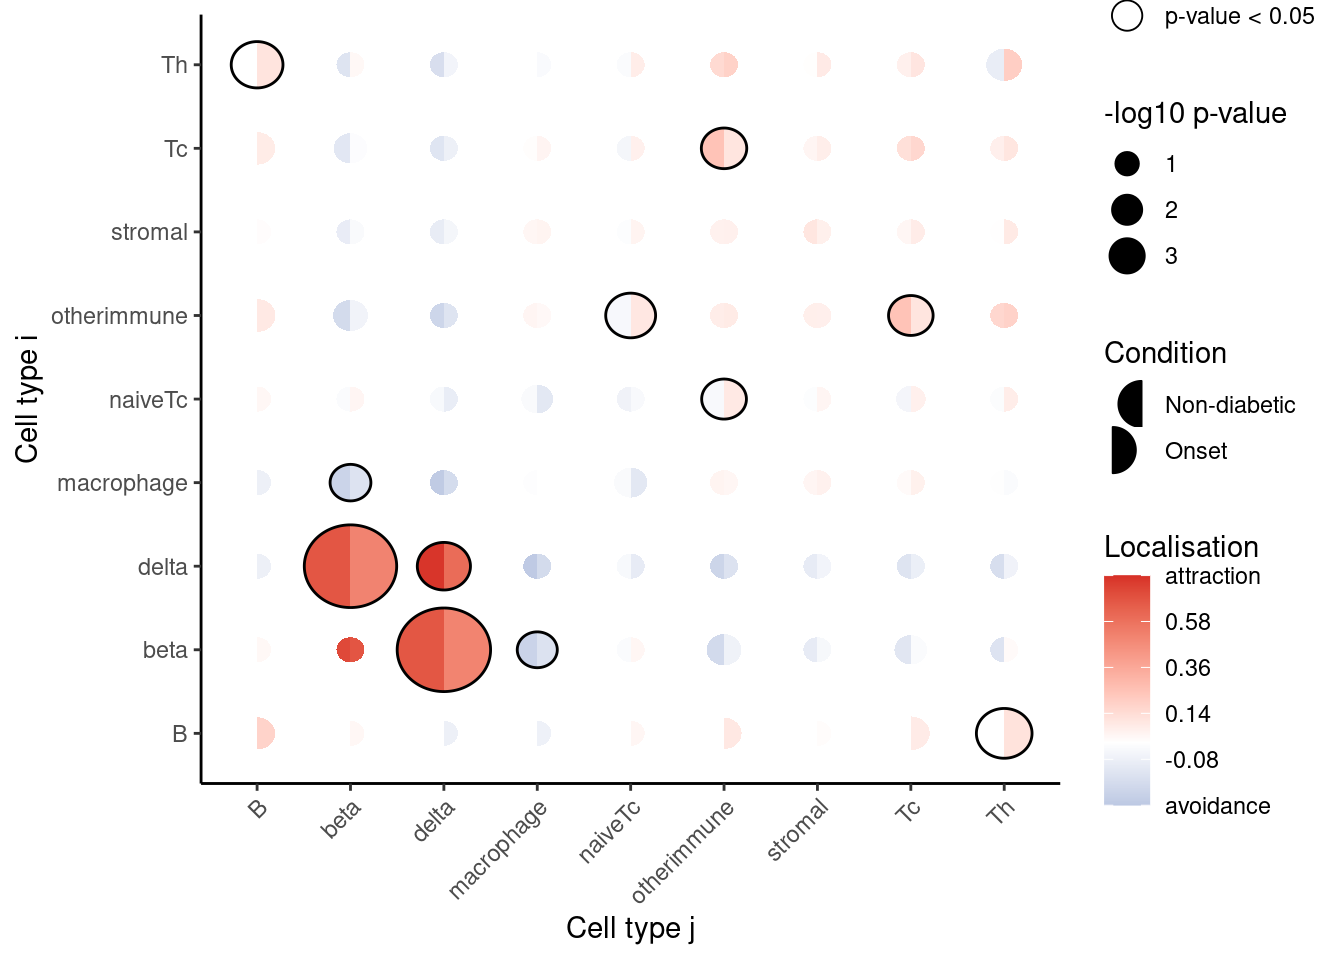
\includegraphics[keepaspectratio]{02-quality_control_files/figure-pdf/unnamed-chunk-3-1.pdf}}

Another method of visualising batch effect is using a dimensionality
reduction technique and visualising how the images separate out on a 2D
plot. If no batch effect is expected, we should see the images largely
overlap with each other.

\begin{Shaded}
\begin{Highlighting}[]
\CommentTok{\# Usually we specify a subset of the original markers which are informative to separating out distinct cell types for the UMAP and clustering.}
\NormalTok{ct\_markers }\OtherTok{\textless{}{-}} \FunctionTok{c}\NormalTok{(}\StringTok{"podoplanin"}\NormalTok{, }\StringTok{"CD13"}\NormalTok{, }\StringTok{"CD31"}\NormalTok{,}
                \StringTok{"panCK"}\NormalTok{, }\StringTok{"CD3"}\NormalTok{, }\StringTok{"CD4"}\NormalTok{, }\StringTok{"CD8a"}\NormalTok{,}
                \StringTok{"CD20"}\NormalTok{, }\StringTok{"CD68"}\NormalTok{, }\StringTok{"CD16"}\NormalTok{, }\StringTok{"CD14"}\NormalTok{, }
                \StringTok{"HLADR"}\NormalTok{, }\StringTok{"CD66a"}\NormalTok{)}

\FunctionTok{set.seed}\NormalTok{(}\DecValTok{51773}\NormalTok{)}
\CommentTok{\# Perform dimension reduction using UMAP.}
\NormalTok{fergusonSPE }\OtherTok{\textless{}{-}}\NormalTok{ scater}\SpecialCharTok{::}\FunctionTok{runUMAP}\NormalTok{(}
\NormalTok{  fergusonSPE,}
  \AttributeTok{subset\_row =}\NormalTok{ ct\_markers,}
  \AttributeTok{exprs\_values =} \StringTok{"counts"}
\NormalTok{)}

\CommentTok{\# Select a subset of images to plot.}
\NormalTok{someImages }\OtherTok{\textless{}{-}} \FunctionTok{unique}\NormalTok{(fergusonSPE}\SpecialCharTok{$}\NormalTok{imageID)[}\FunctionTok{c}\NormalTok{(}\DecValTok{1}\NormalTok{, }\DecValTok{5}\NormalTok{, }\DecValTok{10}\NormalTok{, }\DecValTok{20}\NormalTok{, }\DecValTok{30}\NormalTok{, }\DecValTok{40}\NormalTok{)]}

\CommentTok{\# UMAP by imageID.}
\NormalTok{scater}\SpecialCharTok{::}\FunctionTok{plotReducedDim}\NormalTok{(}
\NormalTok{  fergusonSPE[, fergusonSPE}\SpecialCharTok{$}\NormalTok{imageID }\SpecialCharTok{\%in\%}\NormalTok{ someImages],}
  \AttributeTok{dimred =} \StringTok{"UMAP"}\NormalTok{,}
  \AttributeTok{colour\_by =} \StringTok{"imageID"}
\NormalTok{)}
\end{Highlighting}
\end{Shaded}

\pandocbounded{\includegraphics[keepaspectratio]{02-quality_control_files/figure-pdf/unnamed-chunk-4-1.pdf}}

We can observe that from both our density plot and the UMAP, that there
exists some level of batch effect in our dataset. \texttt{simpleSeg}
also provides functionality for correcting image-level variability,
using the \texttt{normalizeCells()} function.

In the \texttt{normalizeCells()} function, we specify the following
parameters. \texttt{transformation} is an optional argument which
specifies the function to be applied to the data. We do not apply an
arcsinh transformation here, as we already apply a square root transform
in the \texttt{simpleSeg()} function.
\texttt{method\ =\ c("trim99",\ "mean",\ PC1")} is an optional argument
which specifies the normalisation method/s to be performed. A
comprehensive table of methods is provided below.
\texttt{assayIn\ =\ "counts"} is a required argument which specifies
what the assay you'll be taking the intensity data from is named. In our
context, this is called \texttt{counts}.

\begin{longtable}[]{@{}
  >{\raggedright\arraybackslash}p{(\linewidth - 4\tabcolsep) * \real{0.2500}}
  >{\centering\arraybackslash}p{(\linewidth - 4\tabcolsep) * \real{0.3750}}
  >{\centering\arraybackslash}p{(\linewidth - 4\tabcolsep) * \real{0.3750}}@{}}
\toprule\noalign{}
\begin{minipage}[b]{\linewidth}\raggedright
Method
\end{minipage} & \begin{minipage}[b]{\linewidth}\centering
Description
\end{minipage} & \begin{minipage}[b]{\linewidth}\centering
\end{minipage} \\
\midrule\noalign{}
\endhead
\bottomrule\noalign{}
\endlastfoot
{``mean''} & {Divides the marker cellular marker intensities by their
mean.} & \\
{``minMax''} & {Subtracts the minimum value and scales markers between 0
and 1.} & \\
{``trim99''} & {Sets the highest 1\% of values to the value of the 99th
percentile.`} & \\
{``PC1''} & {Removes the 1st principal component) can be performed with
one call of the function, in the order specified by the user.} & \\
\end{longtable}

This modified data is then stored in the \texttt{norm} assay by default,
but can be changed using the \texttt{assayOut} parameter.

\begin{Shaded}
\begin{Highlighting}[]
\CommentTok{\# Leave out the nuclei markers from our normalisation process. }
\NormalTok{useMarkers }\OtherTok{\textless{}{-}} \FunctionTok{rownames}\NormalTok{(fergusonSPE)[}\SpecialCharTok{!}\FunctionTok{rownames}\NormalTok{(fergusonSPE) }\SpecialCharTok{\%in\%} \FunctionTok{c}\NormalTok{(}\StringTok{"DNA1"}\NormalTok{, }\StringTok{"DNA2"}\NormalTok{, }\StringTok{"HH3"}\NormalTok{)]}

\CommentTok{\# Transform and normalise the marker expression of each cell type.}
\NormalTok{fergusonSPE }\OtherTok{\textless{}{-}} \FunctionTok{normalizeCells}\NormalTok{(fergusonSPE,}
                        \AttributeTok{markers =}\NormalTok{ useMarkers,}
                        \AttributeTok{transformation =} \ConstantTok{NULL}\NormalTok{,}
                        \AttributeTok{method =} \FunctionTok{c}\NormalTok{(}\StringTok{"trim99"}\NormalTok{, }\StringTok{"mean"}\NormalTok{, }\StringTok{"PC1"}\NormalTok{),}
                        \AttributeTok{assayIn =} \StringTok{"counts"}\NormalTok{,}
                        \AttributeTok{cores =}\NormalTok{ nCores}
\NormalTok{)}
\end{Highlighting}
\end{Shaded}

We can then plot the same density curve where we can see that this
normalised data appears more bimodal where we can at least observe a
clear CD3+ peak at 1.00, and a CD3- peak at around 0.3, and the images
overlap much more strongly.

\begin{Shaded}
\begin{Highlighting}[]
\CommentTok{\# Plot densities of CD3 for each image}
\NormalTok{fergusonSPE }\SpecialCharTok{|\textgreater{}} 
  \FunctionTok{join\_features}\NormalTok{(}\AttributeTok{features =} \FunctionTok{rownames}\NormalTok{(fergusonSPE), }\AttributeTok{shape =} \StringTok{"wide"}\NormalTok{, }\AttributeTok{assay =} \StringTok{"norm"}\NormalTok{) }\SpecialCharTok{|\textgreater{}} 
  \FunctionTok{ggplot}\NormalTok{(}\FunctionTok{aes}\NormalTok{(}\AttributeTok{x =}\NormalTok{ CD3, }\AttributeTok{colour =}\NormalTok{ imageID)) }\SpecialCharTok{+} 
  \FunctionTok{geom\_density}\NormalTok{() }\SpecialCharTok{+} 
  \FunctionTok{theme}\NormalTok{(}\AttributeTok{legend.position =} \StringTok{"none"}\NormalTok{)}
\end{Highlighting}
\end{Shaded}

\pandocbounded{\includegraphics[keepaspectratio]{02-quality_control_files/figure-pdf/unnamed-chunk-6-1.pdf}}

We can also visualise the effect of normalisation on the UMAP, where our
images now overlap much more strongly with each other.

\begin{Shaded}
\begin{Highlighting}[]
\FunctionTok{set.seed}\NormalTok{(}\DecValTok{51773}\NormalTok{)}
\CommentTok{\# Perform dimension reduction using UMAP.}
\NormalTok{fergusonSPE }\OtherTok{\textless{}{-}}\NormalTok{ scater}\SpecialCharTok{::}\FunctionTok{runUMAP}\NormalTok{(}
\NormalTok{  fergusonSPE,}
  \AttributeTok{subset\_row =}\NormalTok{ ct\_markers,}
  \AttributeTok{exprs\_values =} \StringTok{"norm"}\NormalTok{,}
  \AttributeTok{name =} \StringTok{"normUMAP"}
\NormalTok{)}

\NormalTok{someImages }\OtherTok{\textless{}{-}} \FunctionTok{unique}\NormalTok{(fergusonSPE}\SpecialCharTok{$}\NormalTok{imageID)[}\FunctionTok{c}\NormalTok{(}\DecValTok{1}\NormalTok{, }\DecValTok{5}\NormalTok{, }\DecValTok{10}\NormalTok{, }\DecValTok{20}\NormalTok{, }\DecValTok{30}\NormalTok{, }\DecValTok{40}\NormalTok{)]}

\CommentTok{\# UMAP by imageID.}
\NormalTok{scater}\SpecialCharTok{::}\FunctionTok{plotReducedDim}\NormalTok{(}
\NormalTok{  fergusonSPE[, fergusonSPE}\SpecialCharTok{$}\NormalTok{imageID }\SpecialCharTok{\%in\%}\NormalTok{ someImages],}
  \AttributeTok{dimred =} \StringTok{"normUMAP"}\NormalTok{,}
  \AttributeTok{colour\_by =} \StringTok{"imageID"}
\NormalTok{)}
\end{Highlighting}
\end{Shaded}

\pandocbounded{\includegraphics[keepaspectratio]{02-quality_control_files/figure-pdf/unnamed-chunk-7-1.pdf}}

\section{scMerge: Combining multiple spatial
datasets}\label{scmerge-combining-multiple-spatial-datasets}

A common question that pops up when analysing spatial datasets is:

Can I combine multiple spatial datasets?

\section{sessionInfo}\label{sessioninfo-1}

\begin{Shaded}
\begin{Highlighting}[]
\FunctionTok{sessionInfo}\NormalTok{()}
\end{Highlighting}
\end{Shaded}

\begin{verbatim}
R version 4.4.1 (2024-06-14)
Platform: x86_64-pc-linux-gnu
Running under: Debian GNU/Linux 12 (bookworm)

Matrix products: default
BLAS:   /usr/lib/x86_64-linux-gnu/openblas-pthread/libblas.so.3 
LAPACK: /usr/lib/x86_64-linux-gnu/openblas-pthread/libopenblasp-r0.3.21.so;  LAPACK version 3.11.0

locale:
 [1] LC_CTYPE=C.UTF-8       LC_NUMERIC=C           LC_TIME=C.UTF-8       
 [4] LC_COLLATE=C.UTF-8     LC_MONETARY=C.UTF-8    LC_MESSAGES=C.UTF-8   
 [7] LC_PAPER=C.UTF-8       LC_NAME=C              LC_ADDRESS=C          
[10] LC_TELEPHONE=C         LC_MEASUREMENT=C.UTF-8 LC_IDENTIFICATION=C   

time zone: Australia/Sydney
tzcode source: system (glibc)

attached base packages:
[1] stats4    stats     graphics  grDevices utils     datasets  methods  
[8] base     

other attached packages:
 [1] SpatialDatasets_1.4.0           SpatialExperiment_1.16.0       
 [3] ExperimentHub_2.14.0            AnnotationHub_3.14.0           
 [5] BiocFileCache_2.14.0            dbplyr_2.5.0                   
 [7] scater_1.34.0                   scuttle_1.16.0                 
 [9] simpleSeg_1.8.0                 ggplot2_3.5.1                  
[11] ttservice_0.4.1                 tidyr_1.3.1                    
[13] dplyr_1.1.4                     tidySingleCellExperiment_1.16.0
[15] SingleCellExperiment_1.28.1     SummarizedExperiment_1.36.0    
[17] Biobase_2.66.0                  GenomicRanges_1.58.0           
[19] GenomeInfoDb_1.42.0             IRanges_2.40.0                 
[21] S4Vectors_0.44.0                BiocGenerics_0.52.0            
[23] MatrixGenerics_1.18.0           matrixStats_1.4.1              

loaded via a namespace (and not attached):
  [1] RColorBrewer_1.1-3      rstudioapi_0.17.1       jsonlite_1.8.9         
  [4] magrittr_2.0.3          spatstat.utils_3.1-1    ggbeeswarm_0.7.2       
  [7] magick_2.8.5            farver_2.1.2            rmarkdown_2.29         
 [10] zlibbioc_1.52.0         vctrs_0.6.5             memoise_2.0.1          
 [13] RCurl_1.98-1.16         terra_1.7-83            svgPanZoom_0.3.4       
 [16] tinytex_0.54            htmltools_0.5.8.1       S4Arrays_1.6.0         
 [19] curl_6.0.1              BiocNeighbors_2.0.0     raster_3.6-30          
 [22] Rhdf5lib_1.28.0         SparseArray_1.6.0       rhdf5_2.50.0           
 [25] htmlwidgets_1.6.4       cachem_1.1.0            plotly_4.10.4          
 [28] mime_0.12               lifecycle_1.0.4         pkgconfig_2.0.3        
 [31] rsvd_1.0.5              Matrix_1.7-1            R6_2.5.1               
 [34] fastmap_1.2.0           GenomeInfoDbData_1.2.13 shiny_1.9.1            
 [37] digest_0.6.37           colorspace_2.1-1        AnnotationDbi_1.68.0   
 [40] irlba_2.3.5.1           RSQLite_2.3.7           beachmat_2.22.0        
 [43] labeling_0.4.3          filelock_1.0.3          fansi_1.0.6            
 [46] nnls_1.6                httr_1.4.7              polyclip_1.10-7        
 [49] abind_1.4-8             compiler_4.4.1          bit64_4.5.2            
 [52] withr_3.0.2             tiff_0.1-12             BiocParallel_1.40.0    
 [55] DBI_1.2.3               viridis_0.6.5           HDF5Array_1.34.0       
 [58] cytomapper_1.18.0       rappdirs_0.3.3          DelayedArray_0.32.0    
 [61] rjson_0.2.23            tools_4.4.1             vipor_0.4.7            
 [64] beeswarm_0.4.0          httpuv_1.6.15           glue_1.8.0             
 [67] EBImage_4.48.0          rhdf5filters_1.18.0     promises_1.3.0         
 [70] grid_4.4.1              generics_0.1.3          gtable_0.3.6           
 [73] spatstat.data_3.1-2     data.table_1.16.2       BiocSingular_1.22.0    
 [76] ScaledMatrix_1.14.0     sp_2.1-4                utf8_1.2.4             
 [79] XVector_0.46.0          RcppAnnoy_0.0.22        spatstat.geom_3.3-3    
 [82] BiocVersion_3.20.0      ggrepel_0.9.6           pillar_1.9.0           
 [85] stringr_1.5.1           later_1.3.2             lattice_0.22-6         
 [88] bit_4.5.0               deldir_2.0-4            tidyselect_1.2.1       
 [91] locfit_1.5-9.10         Biostrings_2.74.0       knitr_1.49             
 [94] gridExtra_2.3           svglite_2.1.3           xfun_0.49              
 [97] shinydashboard_0.7.2    stringi_1.8.4           UCSC.utils_1.2.0       
[100] fftwtools_0.9-11        yaml_2.3.10             lazyeval_0.2.2         
[103] evaluate_1.0.1          codetools_0.2-20        tibble_3.2.1           
[106] BiocManager_1.30.25     cli_3.6.3               uwot_0.2.2             
[109] xtable_1.8-4            systemfonts_1.1.0       munsell_0.5.1          
[112] Rcpp_1.0.13-1           png_0.1-8               spatstat.univar_3.1-1  
[115] parallel_4.4.1          ellipsis_0.3.2          blob_1.2.4             
[118] jpeg_0.1-10             bitops_1.0-9            viridisLite_0.4.2      
[121] scales_1.3.0            purrr_1.0.2             crayon_1.5.3           
[124] rlang_1.1.4             cowplot_1.1.3           KEGGREST_1.46.0        
\end{verbatim}

\bookmarksetup{startatroot}

\chapter{Cell Annotation}\label{cell-annotation}

Steps:

\begin{enumerate}
\def\labelenumi{\arabic{enumi}.}
\tightlist
\item
  Rationale behind clustering vs annotation
\item
  How to cluster cells (FuseSOM)
\item
  How to annotate clusters (pheatmap)
\item
  How to annotate cells (scClassify)
\item
  How to select a reference dataset (scClassify)
\end{enumerate}

\section{Which package should I use? Clustering vs
Annotation}\label{which-package-should-i-use-clustering-vs-annotation}

Labeling the identity of your cells is a key step in any spatial
processing protocol in order to determine differential cell type
compositions and changes which occur in specific cell types during
disease. However, the method by which this is done can differ from study
to study. Here, we provide two packages capable of either cell type
clustering (\texttt{FuseSOM}) or cell type annotation
(\texttt{scClassify}).

Clustering is an unsupervised method of labelling cells. This means that
an algorithm separates out clusters of cells based purely off their
marker expression, and the subsequent labeling of these clusters must be
done with some biological domain knowledge. Cell annotation is a
supervised method which requires a separate, reference dataset. The
algorithm then uses that reference dataset to determine the identity of
each of your cell types, thereby labelling your cells in the process.
There are advantages and disadvantages to both, and the choice of one or
the other will be discussed in this chapter. First we'll walk through
how to run both of these packages, and then we'll discuss how to choose
between \texttt{FuseSOM} and \texttt{scClassify}

\section{FuseSOM: Cell clustering}\label{fusesom-cell-clustering}

A correlation based multiview self organizing map for the
characterization of cell types (\texttt{FuseSOM}) is a tool for
unsupervised clustering. \texttt{FuseSOM} is robust and achieves high
accuracy by combining a \texttt{Self\ Organizing\ Map} architecture and
a \texttt{Multiview} integration of correlation based metrics to cluster
highly multiplexed in situ imaging cytometry assays. The
\texttt{FuseSOM} pipeline has been streamlined and accepts currently
used data structures including \texttt{SingleCellExperiment} and
\texttt{SpatialExperiment} objects as well as \texttt{DataFrames}.

\subsection{\texorpdfstring{\texttt{FuseSOM} Matrix
Input}{FuseSOM Matrix Input}}\label{fusesom-matrix-input}

If you have a matrix containing expression data that was QCed and
normalised by some other tool, the next step is to run the
\texttt{FuseSOM} algorithm.This can be done by calling the
\texttt{runFuseSOM()} function which takes in the matrix of interest
where the columns are markers and the rows are observations, the makers
of interest (if this is not provided, it is assumed that all columns are
markers), and the number of clusters.

\begin{Shaded}
\begin{Highlighting}[]
\CommentTok{\# load FuseSOM}
\FunctionTok{library}\NormalTok{(FuseSOM)}
\end{Highlighting}
\end{Shaded}

Next we will load in the
\href{https://www.sciencedirect.com/science/article/pii/S0092867421014860?via\%3Dihub}{\texttt{Risom\ et\ al}}
dataset and run it through the FuseSOM pipeline. This dataset profiles
the spatial landscape of ductal carcinoma in situ (DCIS), which is a
pre-invasive lesion that is thought to be a precursor to invasive breast
cancer (IBC). The key conclusion of this manuscript (amongst others) is
that spatial information about cells can be used to predict disease
progression in patients.We will also be using the markers used in the
original study.

\begin{Shaded}
\begin{Highlighting}[]
\CommentTok{\# load in the data}
\FunctionTok{data}\NormalTok{(}\StringTok{"risom\_dat"}\NormalTok{)}

\CommentTok{\# define the markers of interest}
\NormalTok{risomMarkers }\OtherTok{\textless{}{-}} \FunctionTok{c}\NormalTok{(}\StringTok{\textquotesingle{}CD45\textquotesingle{}}\NormalTok{,}\StringTok{\textquotesingle{}SMA\textquotesingle{}}\NormalTok{,}\StringTok{\textquotesingle{}CK7\textquotesingle{}}\NormalTok{,}\StringTok{\textquotesingle{}CK5\textquotesingle{}}\NormalTok{,}\StringTok{\textquotesingle{}VIM\textquotesingle{}}\NormalTok{,}\StringTok{\textquotesingle{}CD31\textquotesingle{}}\NormalTok{,}\StringTok{\textquotesingle{}PanKRT\textquotesingle{}}\NormalTok{,}\StringTok{\textquotesingle{}ECAD\textquotesingle{}}\NormalTok{,}
                   \StringTok{\textquotesingle{}Tryptase\textquotesingle{}}\NormalTok{,}\StringTok{\textquotesingle{}MPO\textquotesingle{}}\NormalTok{,}\StringTok{\textquotesingle{}CD20\textquotesingle{}}\NormalTok{,}\StringTok{\textquotesingle{}CD3\textquotesingle{}}\NormalTok{,}\StringTok{\textquotesingle{}CD8\textquotesingle{}}\NormalTok{,}\StringTok{\textquotesingle{}CD4\textquotesingle{}}\NormalTok{,}\StringTok{\textquotesingle{}CD14\textquotesingle{}}\NormalTok{,}\StringTok{\textquotesingle{}CD68\textquotesingle{}}\NormalTok{,}\StringTok{\textquotesingle{}FAP\textquotesingle{}}\NormalTok{,}
                   \StringTok{\textquotesingle{}CD36\textquotesingle{}}\NormalTok{,}\StringTok{\textquotesingle{}CD11c\textquotesingle{}}\NormalTok{,}\StringTok{\textquotesingle{}HLADRDPDQ\textquotesingle{}}\NormalTok{,}\StringTok{\textquotesingle{}P63\textquotesingle{}}\NormalTok{,}\StringTok{\textquotesingle{}CD44\textquotesingle{}}\NormalTok{)}

\CommentTok{\# we will be using the manual\_gating\_phenotype as the true cell type to gauge }
\CommentTok{\# performance}
\FunctionTok{names}\NormalTok{(risom\_dat)[}\FunctionTok{names}\NormalTok{(risom\_dat) }\SpecialCharTok{==} \StringTok{\textquotesingle{}manual\_gating\_phenotype\textquotesingle{}}\NormalTok{] }\OtherTok{\textless{}{-}} \StringTok{\textquotesingle{}CellType\textquotesingle{}}
\end{Highlighting}
\end{Shaded}

Now that we have loaded the data and define the markers of interest. We
can run the \texttt{FuseSOM} algorithm. We have provided a function
\texttt{runFuseSOM} that runs the pipeline from top to bottom and
returns the cluster labels as well as the \texttt{Self\ Organizing\ Map}
model.

\begin{Shaded}
\begin{Highlighting}[]
\NormalTok{risomRes }\OtherTok{\textless{}{-}} \FunctionTok{runFuseSOM}\NormalTok{(}\AttributeTok{data =}\NormalTok{ risom\_dat, }\AttributeTok{markers =}\NormalTok{ risomMarkers, }
                        \AttributeTok{numClusters =} \DecValTok{23}\NormalTok{)}
\end{Highlighting}
\end{Shaded}

\begin{verbatim}
You have provided a dataset of class data.frame
\end{verbatim}

\begin{verbatim}
Everything looks good. Now running the FuseSOM algorithm
\end{verbatim}

\begin{verbatim}
Now Generating the Self Organizing Map Grid
\end{verbatim}

\begin{verbatim}
Optimal Grid Size is: 8
\end{verbatim}

\begin{verbatim}
Now Running the Self Organizing Map Model
\end{verbatim}

\begin{verbatim}
Now Clustering the Prototypes
\end{verbatim}

\begin{verbatim}
Loading required namespace: fastcluster
\end{verbatim}

\begin{verbatim}
Now Mapping Clusters to the Original Data
\end{verbatim}

\begin{verbatim}
The Prototypes have been Clustered and Mapped Successfully
\end{verbatim}

\begin{verbatim}
The FuseSOM algorithm has completed successfully
\end{verbatim}

Lets look at the distribution of the clusters.

\begin{Shaded}
\begin{Highlighting}[]
\CommentTok{\# get the distribution of the clusters}
\FunctionTok{table}\NormalTok{(risomRes}\SpecialCharTok{$}\NormalTok{clusters)}\SpecialCharTok{/}\FunctionTok{sum}\NormalTok{(}\FunctionTok{table}\NormalTok{(risomRes}\SpecialCharTok{$}\NormalTok{clusters))}
\end{Highlighting}
\end{Shaded}

\begin{verbatim}

  cluster_1  cluster_10  cluster_11  cluster_12  cluster_13  cluster_14 
0.323602021 0.035968538 0.005439775 0.021443334 0.061100586 0.026596050 
 cluster_15  cluster_16  cluster_17  cluster_18  cluster_19   cluster_2 
0.020582156 0.032624297 0.024931106 0.076128143 0.015802618 0.014927087 
 cluster_20  cluster_21  cluster_22  cluster_23   cluster_3   cluster_4 
0.049962682 0.009185900 0.051771156 0.066913538 0.004923068 0.014108968 
  cluster_5   cluster_6   cluster_7   cluster_8   cluster_9 
0.040776783 0.064444827 0.020854863 0.010032725 0.007879780 
\end{verbatim}

Looks like \texttt{cluster\_1} has about \(32\%\) of the cells which is
interesting. Next, lets generate a heatmap of the marker expression for
each cluster.

\begin{Shaded}
\begin{Highlighting}[]
\NormalTok{risomHeat }\OtherTok{\textless{}{-}}\NormalTok{ FuseSOM}\SpecialCharTok{::}\FunctionTok{markerHeatmap}\NormalTok{(}\AttributeTok{data =}\NormalTok{ risom\_dat, }\AttributeTok{markers =}\NormalTok{ risomMarkers,}
                            \AttributeTok{clusters =}\NormalTok{ risomRes}\SpecialCharTok{$}\NormalTok{clusters, }\AttributeTok{clusterMarkers =} \ConstantTok{TRUE}\NormalTok{)}
\end{Highlighting}
\end{Shaded}

\begin{center}
\pandocbounded{\includegraphics[keepaspectratio]{03-cell_annotation_files/figure-pdf/unnamed-chunk-5-1.png}}
\end{center}

\subsection{\texorpdfstring{Using \texttt{FuseSOM} to estimate the
number of
clusters}{Using FuseSOM to estimate the number of clusters}}\label{using-fusesom-to-estimate-the-number-of-clusters}

\texttt{FuseSOM} also provides functionality for estimating the number
of clusters in a dataset using three classes of methods including:

\begin{enumerate}
\def\labelenumi{\arabic{enumi}.}
\tightlist
\item
  Discriminant based method.

  \begin{itemize}
  \tightlist
  \item
    A method developed in house based on discriminant based maximum
    clusterability projection pursuit
  \end{itemize}
\item
  Distance based methods which includes:

  \begin{itemize}
  \tightlist
  \item
    The Gap Statistic
  \item
    The Jump Statistic
  \item
    The Slope Statistic
  \item
    The Within Cluster Dissimilarity Statistic
  \item
    The Silhouette Statistic
  \end{itemize}
\end{enumerate}

We can estimate the number of clusters using the
\texttt{estimateNumCluster}. Run \texttt{help(estimateNumCluster)} to
see it's complete functionality.

\begin{Shaded}
\begin{Highlighting}[]
\CommentTok{\# lets estimate the number of clusters using all the methods}
\CommentTok{\# original clustering has 23 clusters so we will set kseq from 2:25}
\CommentTok{\# we pass it the som model generated in the previous step}
\NormalTok{risomKest }\OtherTok{\textless{}{-}} \FunctionTok{estimateNumCluster}\NormalTok{(}\AttributeTok{data =}\NormalTok{ risomRes}\SpecialCharTok{$}\NormalTok{model, }\AttributeTok{kSeq =} \DecValTok{2}\SpecialCharTok{:}\DecValTok{25}\NormalTok{, }
                                  \AttributeTok{method =} \FunctionTok{c}\NormalTok{(}\StringTok{"Discriminant"}\NormalTok{, }\StringTok{"Distance"}\NormalTok{))}
\end{Highlighting}
\end{Shaded}

\begin{verbatim}
Now Computing the Number of Clusters using Discriminant Analysis
\end{verbatim}

\begin{verbatim}
Now Computing The Number Of Clusters Using Distance Analysis
\end{verbatim}

We can then use this result to determine the best number of clusters for
this dataset based on the different metrics. The \texttt{FuseSOM}
package provides a plotting function (\texttt{optiPlot}) which generates
an elbow plot with the optimal value for the number of clusters for the
distance based methods. See below

\begin{Shaded}
\begin{Highlighting}[]
\CommentTok{\# what is the best number of clusters determined by the discriminant method?}
\CommentTok{\# optimal number of clusters according to the discriminant method is 7}
\NormalTok{risomKest}\SpecialCharTok{$}\NormalTok{Discriminant }
\end{Highlighting}
\end{Shaded}

\begin{verbatim}
[1] 10
\end{verbatim}

\begin{Shaded}
\begin{Highlighting}[]
\CommentTok{\# we can plot the results using the optiplot function}
\NormalTok{pSlope }\OtherTok{\textless{}{-}} \FunctionTok{optiPlot}\NormalTok{(risomKest, }\AttributeTok{method =} \StringTok{\textquotesingle{}slope\textquotesingle{}}\NormalTok{)}
\NormalTok{pSlope}
\end{Highlighting}
\end{Shaded}

\pandocbounded{\includegraphics[keepaspectratio]{03-cell_annotation_files/figure-pdf/unnamed-chunk-7-1.pdf}}

\begin{Shaded}
\begin{Highlighting}[]
\NormalTok{pJump }\OtherTok{\textless{}{-}} \FunctionTok{optiPlot}\NormalTok{(risomKest, }\AttributeTok{method =} \StringTok{\textquotesingle{}jump\textquotesingle{}}\NormalTok{)}
\NormalTok{pJump}
\end{Highlighting}
\end{Shaded}

\pandocbounded{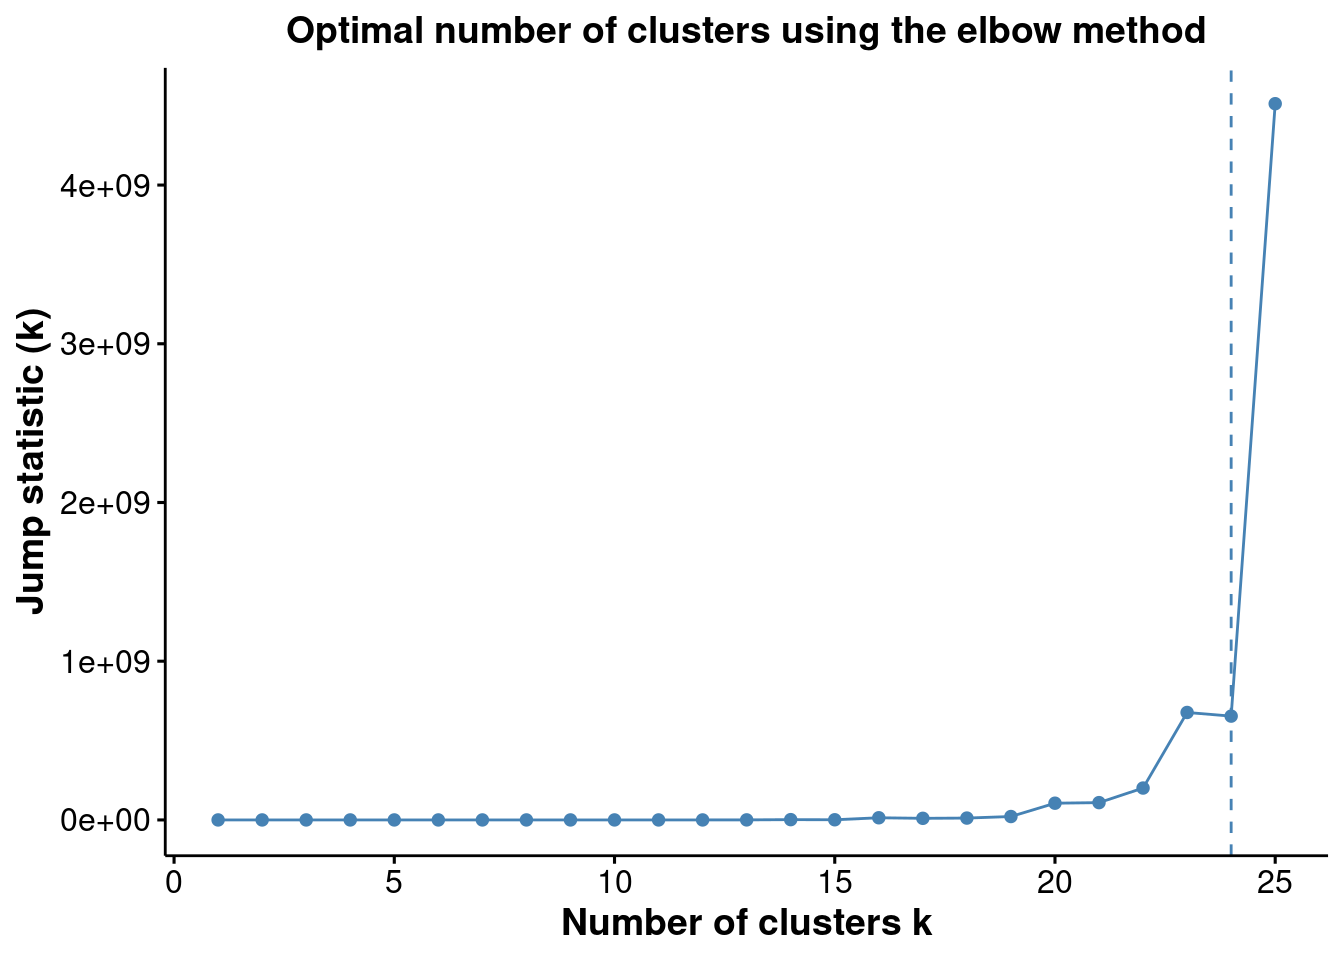
\includegraphics[keepaspectratio]{03-cell_annotation_files/figure-pdf/unnamed-chunk-7-2.pdf}}

\begin{Shaded}
\begin{Highlighting}[]
\NormalTok{pWcd }\OtherTok{\textless{}{-}} \FunctionTok{optiPlot}\NormalTok{(risomKest, }\AttributeTok{method =} \StringTok{\textquotesingle{}wcd\textquotesingle{}}\NormalTok{)}
\NormalTok{pWcd}
\end{Highlighting}
\end{Shaded}

\pandocbounded{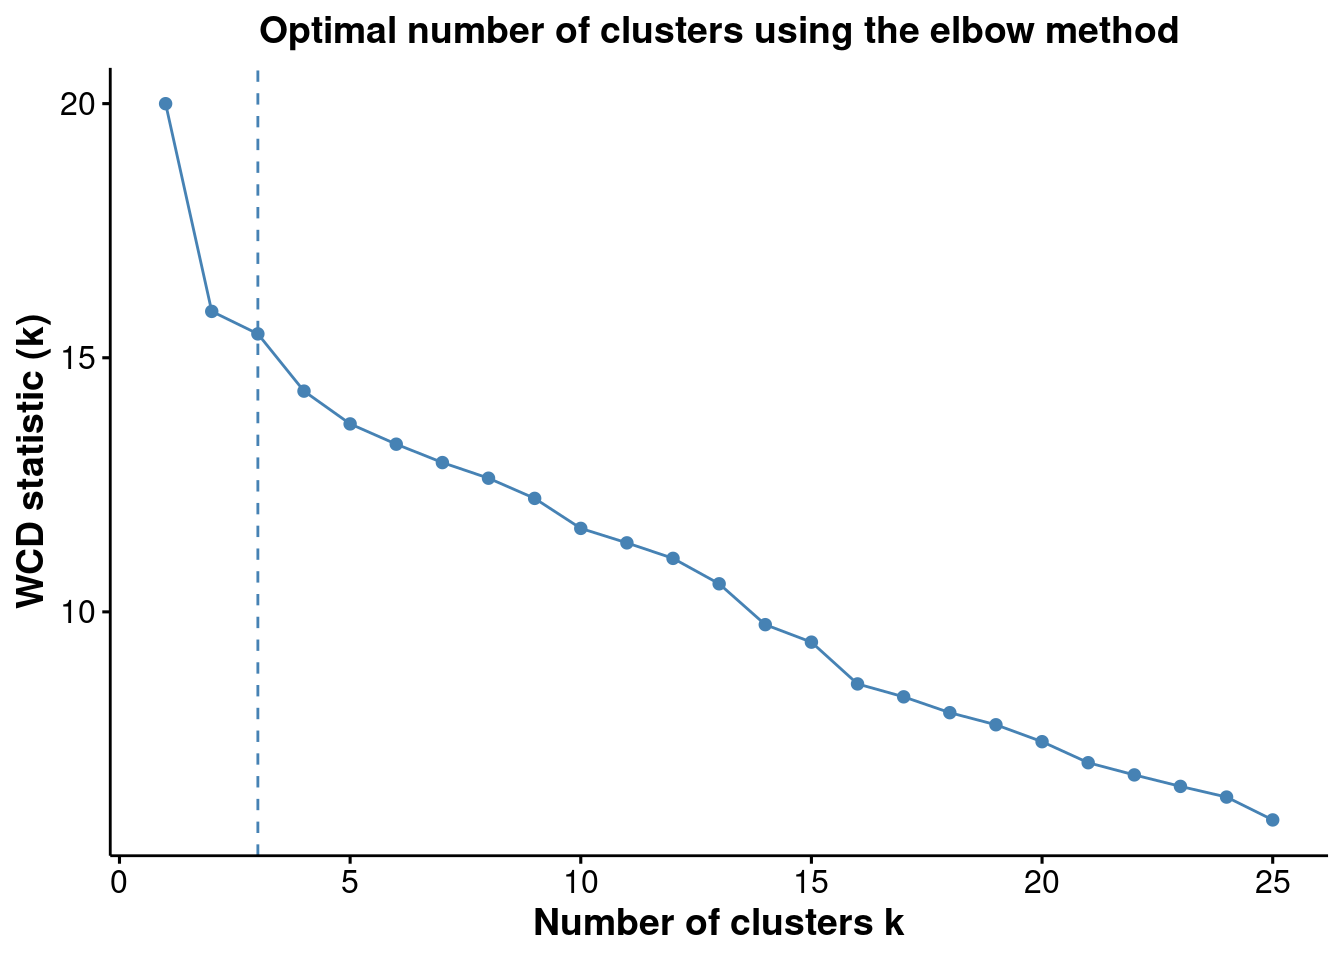
\includegraphics[keepaspectratio]{03-cell_annotation_files/figure-pdf/unnamed-chunk-7-3.pdf}}

\begin{Shaded}
\begin{Highlighting}[]
\NormalTok{pGap }\OtherTok{\textless{}{-}} \FunctionTok{optiPlot}\NormalTok{(risomKest, }\AttributeTok{method =} \StringTok{\textquotesingle{}gap\textquotesingle{}}\NormalTok{)}
\NormalTok{pGap}
\end{Highlighting}
\end{Shaded}

\pandocbounded{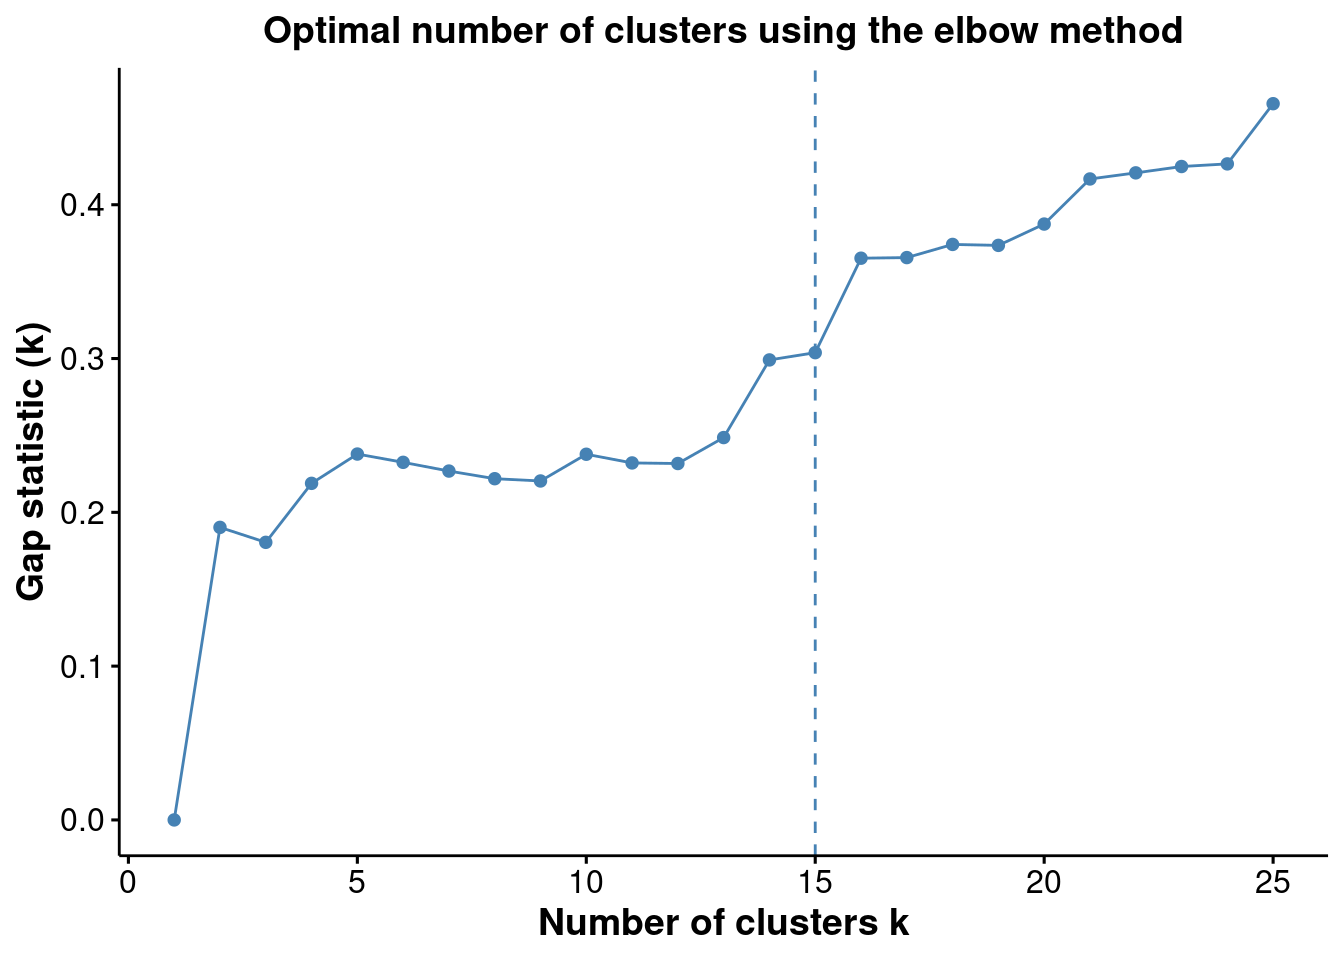
\includegraphics[keepaspectratio]{03-cell_annotation_files/figure-pdf/unnamed-chunk-7-4.pdf}}

\begin{Shaded}
\begin{Highlighting}[]
\NormalTok{pSil }\OtherTok{\textless{}{-}} \FunctionTok{optiPlot}\NormalTok{(risomKest, }\AttributeTok{method =} \StringTok{\textquotesingle{}silhouette\textquotesingle{}}\NormalTok{)}
\NormalTok{pSil}
\end{Highlighting}
\end{Shaded}

\pandocbounded{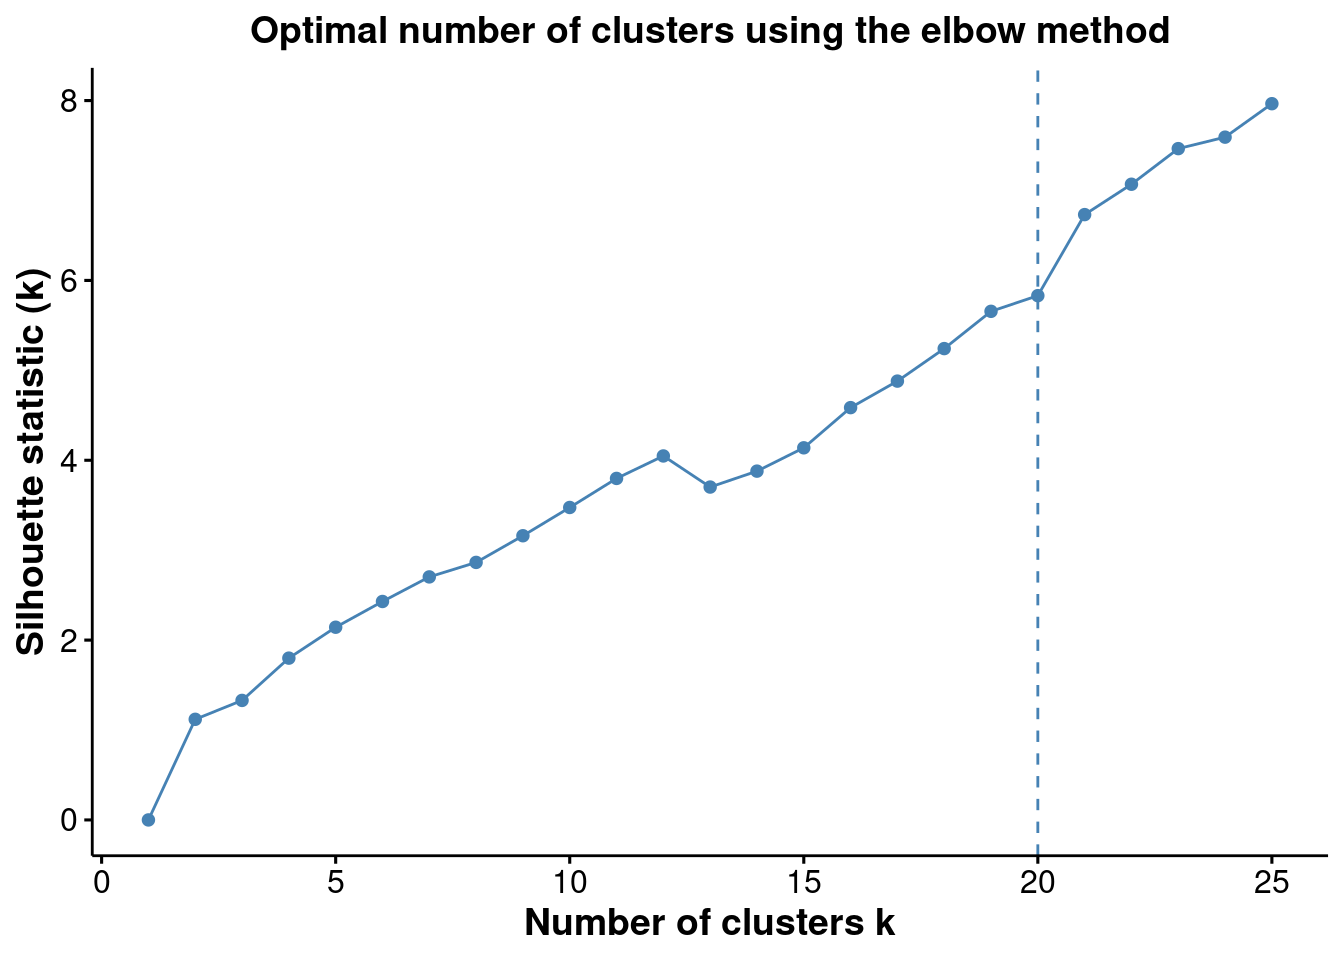
\includegraphics[keepaspectratio]{03-cell_annotation_files/figure-pdf/unnamed-chunk-7-5.pdf}}

From the plots, we see that the \texttt{Jump} statistics almost
perfectly capture the number of clusters. The \texttt{Gap} method is a
close second with \(15\) clusters. All the other methods significantly
underestimates the number of clusters.

\subsection{\texorpdfstring{\texttt{FuseSOM} Single Cell Epxeriment
object as
input.}{FuseSOM Single Cell Epxeriment object as input.}}\label{fusesom-single-cell-epxeriment-object-as-input.}

The \texttt{FuseSOM} algorithm is also equipped to take in a
\texttt{SingleCellExperiment} object as input. The results of the
pipeline will be written to either the metada or the colData fields. See
below.

First we create a \texttt{SingleCellExperiment} object

\begin{Shaded}
\begin{Highlighting}[]
\FunctionTok{library}\NormalTok{(SingleCellExperiment)}

\CommentTok{\# create a singelcellexperiment object}
\NormalTok{colDat }\OtherTok{\textless{}{-}}\NormalTok{ risom\_dat[, }\FunctionTok{setdiff}\NormalTok{(}\FunctionTok{colnames}\NormalTok{(risom\_dat), risomMarkers)]}
\NormalTok{sce }\OtherTok{\textless{}{-}} \FunctionTok{SingleCellExperiment}\NormalTok{(}\AttributeTok{assays =} \FunctionTok{list}\NormalTok{(}\AttributeTok{counts =} \FunctionTok{t}\NormalTok{(risom\_dat)),}
                                 \AttributeTok{colData =}\NormalTok{ colDat)}

\NormalTok{sce}
\end{Highlighting}
\end{Shaded}

\begin{verbatim}
class: SingleCellExperiment 
dim: 23 69672 
metadata(0):
assays(1): counts
rownames(23): CD45 SMA ... CD44 CellType
rowData names(0):
colnames: NULL
colData names(1): X
reducedDimNames(0):
mainExpName: NULL
altExpNames(0):
\end{verbatim}

Next we pass it to the \texttt{runFuseSOM()} function. Here, we can
provide the assay in which the data is stored and what name to store the
clusters under in the colData section. Note that the
\texttt{Self\ Organizing\ Map} that is generated will be stored in the
metadata field.

\begin{Shaded}
\begin{Highlighting}[]
\NormalTok{risomRessce }\OtherTok{\textless{}{-}} \FunctionTok{runFuseSOM}\NormalTok{(sce, }\AttributeTok{markers =}\NormalTok{ risomMarkers, }\AttributeTok{assay =} \StringTok{\textquotesingle{}counts\textquotesingle{}}\NormalTok{, }
                      \AttributeTok{numClusters =} \DecValTok{23}\NormalTok{, }\AttributeTok{verbose =} \ConstantTok{FALSE}\NormalTok{)}
\end{Highlighting}
\end{Shaded}

\begin{verbatim}
You have provided a dataset of class SingleCellExperiment
\end{verbatim}

\begin{verbatim}
Everything looks good. Now running the FuseSOM algorithm
\end{verbatim}

\begin{verbatim}
Now Generating the Self Organizing Map Grid
\end{verbatim}

\begin{verbatim}
Optimal Grid Size is: 8
\end{verbatim}

\begin{verbatim}
Now Running the Self Organizing Map Model
\end{verbatim}

\begin{verbatim}
Now Clustering the Prototypes
\end{verbatim}

\begin{verbatim}
Now Mapping Clusters to the Original Data
\end{verbatim}

\begin{verbatim}
The Prototypes have been Clustered and Mapped Successfully
\end{verbatim}

\begin{verbatim}
The FuseSOM algorithm has completed successfully
\end{verbatim}

\begin{Shaded}
\begin{Highlighting}[]
\FunctionTok{colnames}\NormalTok{(}\FunctionTok{colData}\NormalTok{(risomRessce))}
\end{Highlighting}
\end{Shaded}

\begin{verbatim}
[1] "X"        "clusters"
\end{verbatim}

\begin{Shaded}
\begin{Highlighting}[]
\FunctionTok{names}\NormalTok{(}\FunctionTok{metadata}\NormalTok{(risomRessce))}
\end{Highlighting}
\end{Shaded}

\begin{verbatim}
[1] "SOM"
\end{verbatim}

Notice how the there is now a clusters column in the colData and SOM
field in the metadata. You can run this function again with a new set of
cluster number. If you provide a new name for the clusters, it will be
stored under that new column, else, it will overwrite the current
clusters column. Running it again on the same object will overwrite the
SOM field in the metadata.

Just like before, lets plot the heatmap of the resulting clusters across
all markers.

\begin{Shaded}
\begin{Highlighting}[]
\NormalTok{data }\OtherTok{\textless{}{-}}\NormalTok{ risom\_dat[, risomMarkers] }\CommentTok{\# get the original data used}
\NormalTok{clusters }\OtherTok{\textless{}{-}} \FunctionTok{colData}\NormalTok{(risomRessce)}\SpecialCharTok{$}\NormalTok{clusters }\CommentTok{\# extract the clusters from the sce object}
\CommentTok{\# generate the heatmap}
\NormalTok{risomHeatsce }\OtherTok{\textless{}{-}} \FunctionTok{markerHeatmap}\NormalTok{(}\AttributeTok{data =}\NormalTok{ risom\_dat, }\AttributeTok{markers =}\NormalTok{ risomMarkers,}
                            \AttributeTok{clusters =}\NormalTok{ clusters, }\AttributeTok{clusterMarkers =} \ConstantTok{TRUE}\NormalTok{)}
\end{Highlighting}
\end{Shaded}

\pandocbounded{\includegraphics[keepaspectratio]{03-cell_annotation_files/figure-pdf/unnamed-chunk-10-1.pdf}}

\subsection{\texorpdfstring{Using \texttt{FuseSOM} to estimate the
number of clusters for single cell experiment
objects}{Using FuseSOM to estimate the number of clusters for single cell experiment objects}}\label{using-fusesom-to-estimate-the-number-of-clusters-for-single-cell-experiment-objects}

Just like before, we can estimate the number of clusters

\begin{Shaded}
\begin{Highlighting}[]
\CommentTok{\# lets estimate the number of clusters using all the methods}
\CommentTok{\# original clustering has 23 clusters so we will set kseq from 2:25}
\CommentTok{\# now we pass it a singlecellexperiment object instead of the som model as before}
\CommentTok{\# this will return a singelcellexperiment object where the metatdata contains the}
\CommentTok{\# cluster estimation information}
\NormalTok{risomRessce }\OtherTok{\textless{}{-}} \FunctionTok{estimateNumCluster}\NormalTok{(}\AttributeTok{data =}\NormalTok{ risomRessce, }\AttributeTok{kSeq =} \DecValTok{2}\SpecialCharTok{:}\DecValTok{25}\NormalTok{, }
                                  \AttributeTok{method =} \FunctionTok{c}\NormalTok{(}\StringTok{"Discriminant"}\NormalTok{, }\StringTok{"Distance"}\NormalTok{))}
\end{Highlighting}
\end{Shaded}

\begin{verbatim}
You have provided a dataset of class: SingleCellExperiment
\end{verbatim}

\begin{verbatim}
Now Computing the Number of Clusters using Discriminant Analysis
\end{verbatim}

\begin{verbatim}
Now Computing The Number Of Clusters Using Distance Analysis
\end{verbatim}

\begin{Shaded}
\begin{Highlighting}[]
\FunctionTok{names}\NormalTok{(}\FunctionTok{metadata}\NormalTok{(risomRessce))}
\end{Highlighting}
\end{Shaded}

\begin{verbatim}
[1] "SOM"               "clusterEstimation"
\end{verbatim}

Notice how the metadata now contains a \texttt{clusterEstimation} field
which holds the results from the \texttt{estimateNumCluster()} function

We can assess the results in a similar fashion as before

\begin{Shaded}
\begin{Highlighting}[]
\CommentTok{\# what is the best number of clusters determined by the discriminant method?}
\CommentTok{\# optimal number of clusters according to the discriminant method is 8}
\FunctionTok{metadata}\NormalTok{(risomRessce)}\SpecialCharTok{$}\NormalTok{clusterEstimation}\SpecialCharTok{$}\NormalTok{Discriminant }
\end{Highlighting}
\end{Shaded}

\begin{verbatim}
[1] 7
\end{verbatim}

\begin{Shaded}
\begin{Highlighting}[]
\CommentTok{\# we can plot the results using the optiplot function}
\NormalTok{pSlope }\OtherTok{\textless{}{-}} \FunctionTok{optiPlot}\NormalTok{(risomRessce, }\AttributeTok{method =} \StringTok{\textquotesingle{}slope\textquotesingle{}}\NormalTok{)}
\end{Highlighting}
\end{Shaded}

\begin{verbatim}
You have provided a dataset of class: SingleCellExperiment
\end{verbatim}

\begin{Shaded}
\begin{Highlighting}[]
\NormalTok{pSlope}
\end{Highlighting}
\end{Shaded}

\begin{center}
\pandocbounded{\includegraphics[keepaspectratio]{03-cell_annotation_files/figure-pdf/unnamed-chunk-12-1.png}}
\end{center}

\begin{Shaded}
\begin{Highlighting}[]
\NormalTok{pJump }\OtherTok{\textless{}{-}} \FunctionTok{optiPlot}\NormalTok{(risomRessce, }\AttributeTok{method =} \StringTok{\textquotesingle{}jump\textquotesingle{}}\NormalTok{)}
\end{Highlighting}
\end{Shaded}

\begin{verbatim}
You have provided a dataset of class: SingleCellExperiment
\end{verbatim}

\begin{Shaded}
\begin{Highlighting}[]
\NormalTok{pJump}
\end{Highlighting}
\end{Shaded}

\begin{center}
\pandocbounded{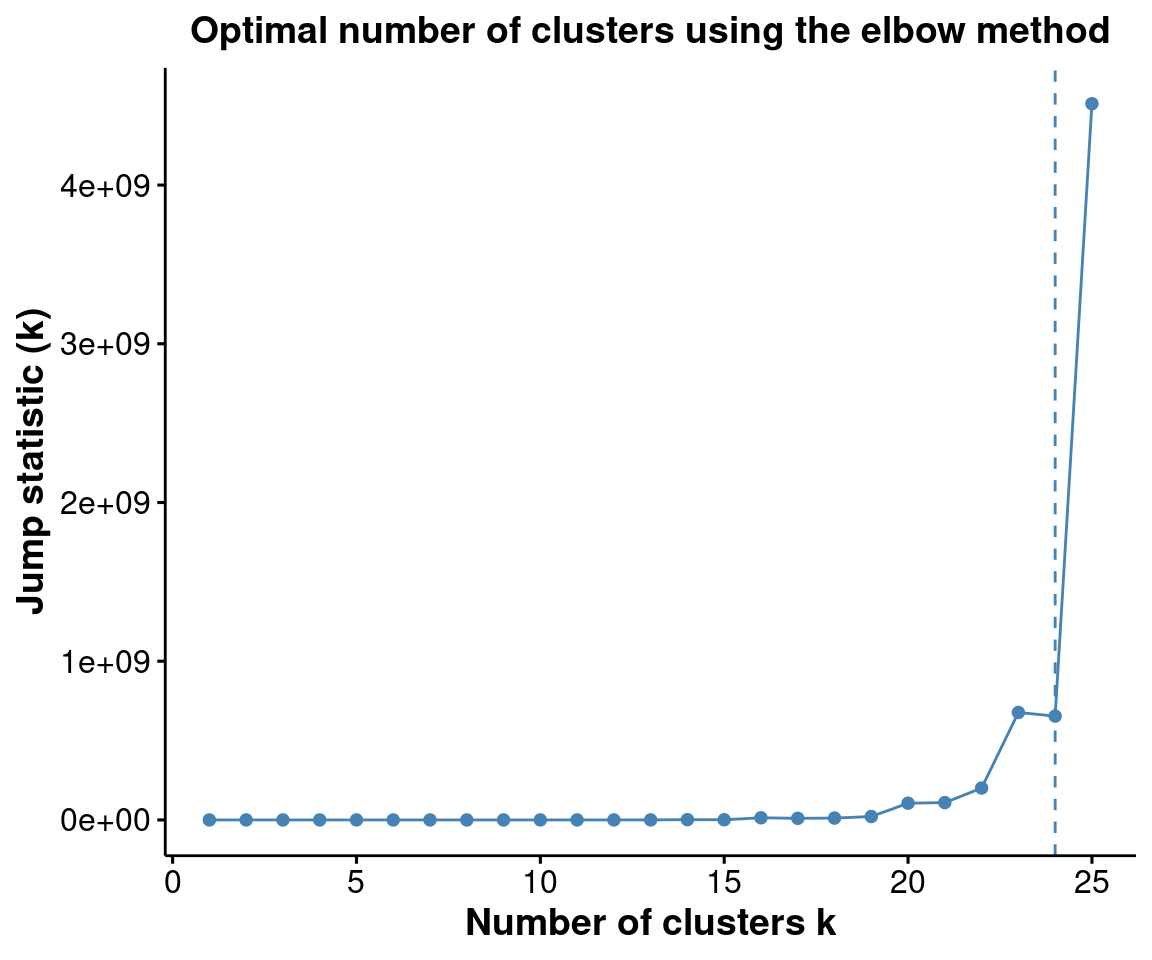
\includegraphics[keepaspectratio]{03-cell_annotation_files/figure-pdf/unnamed-chunk-12-2.png}}
\end{center}

\begin{Shaded}
\begin{Highlighting}[]
\NormalTok{pWcd }\OtherTok{\textless{}{-}} \FunctionTok{optiPlot}\NormalTok{(risomRessce, }\AttributeTok{method =} \StringTok{\textquotesingle{}wcd\textquotesingle{}}\NormalTok{)}
\end{Highlighting}
\end{Shaded}

\begin{verbatim}
You have provided a dataset of class: SingleCellExperiment
\end{verbatim}

\begin{Shaded}
\begin{Highlighting}[]
\NormalTok{pWcd}
\end{Highlighting}
\end{Shaded}

\begin{center}
\pandocbounded{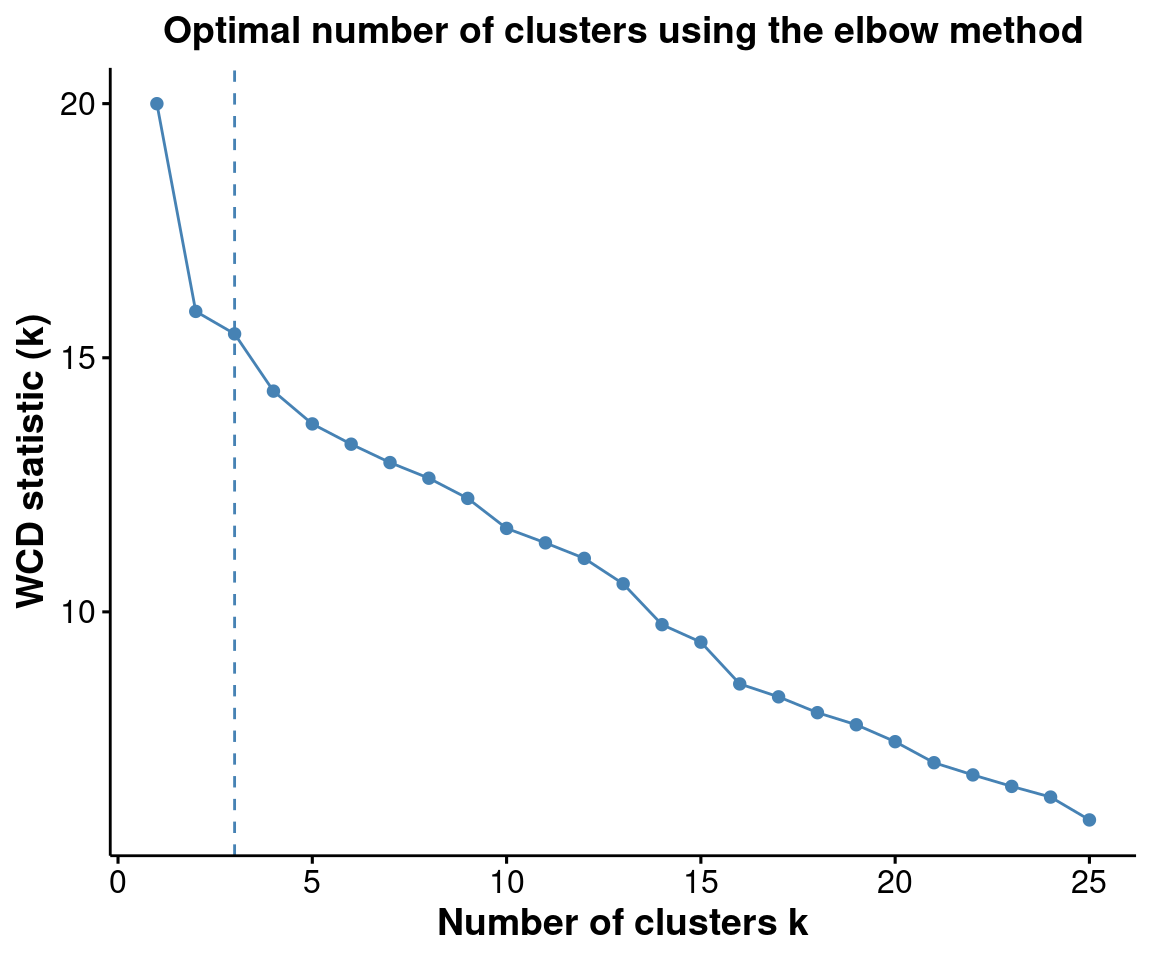
\includegraphics[keepaspectratio]{03-cell_annotation_files/figure-pdf/unnamed-chunk-12-3.png}}
\end{center}

\begin{Shaded}
\begin{Highlighting}[]
\NormalTok{pGap }\OtherTok{\textless{}{-}} \FunctionTok{optiPlot}\NormalTok{(risomRessce, }\AttributeTok{method =} \StringTok{\textquotesingle{}gap\textquotesingle{}}\NormalTok{)}
\end{Highlighting}
\end{Shaded}

\begin{verbatim}
You have provided a dataset of class: SingleCellExperiment
\end{verbatim}

\begin{Shaded}
\begin{Highlighting}[]
\NormalTok{pGap}
\end{Highlighting}
\end{Shaded}

\begin{center}
\pandocbounded{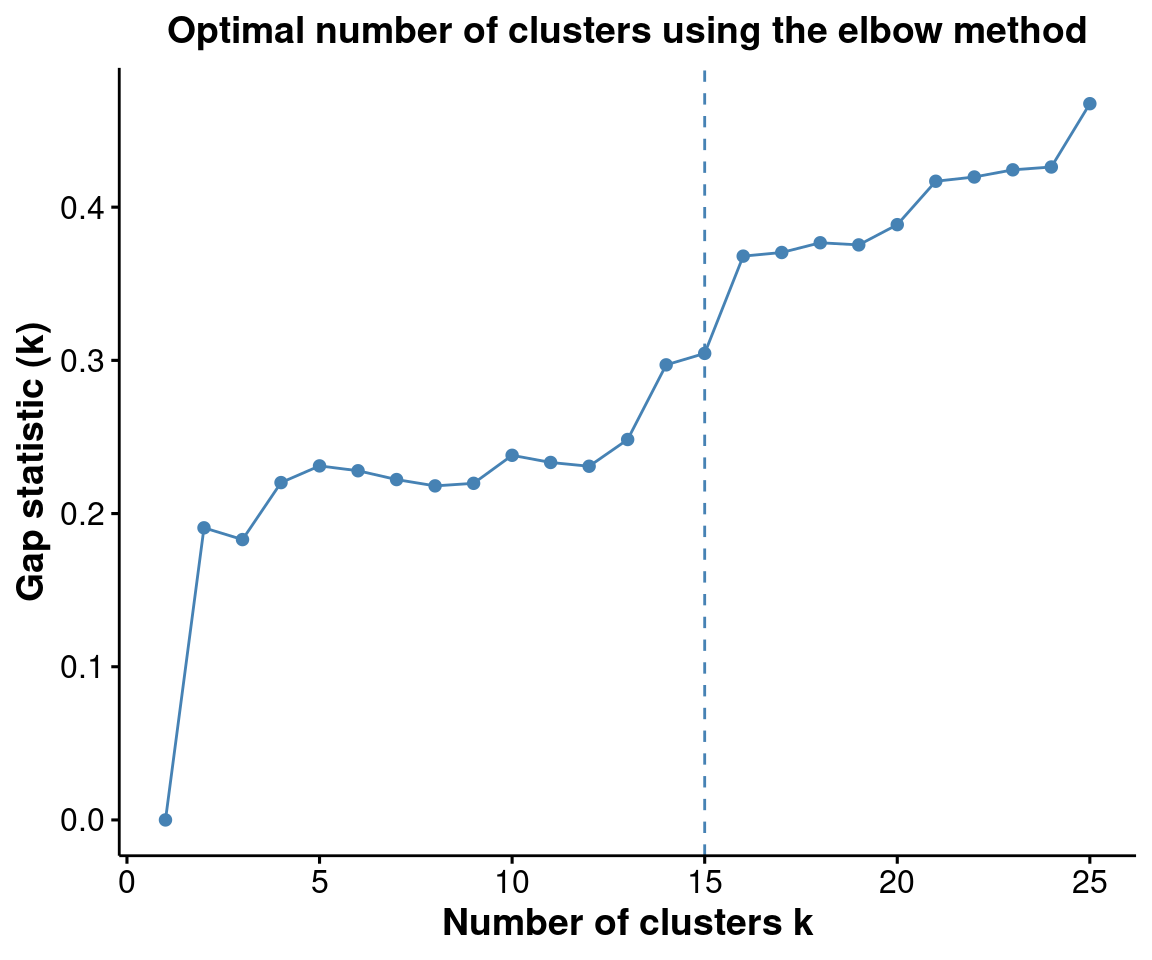
\includegraphics[keepaspectratio]{03-cell_annotation_files/figure-pdf/unnamed-chunk-12-4.png}}
\end{center}

\begin{Shaded}
\begin{Highlighting}[]
\NormalTok{pSil }\OtherTok{\textless{}{-}} \FunctionTok{optiPlot}\NormalTok{(risomRessce, }\AttributeTok{method =} \StringTok{\textquotesingle{}silhouette\textquotesingle{}}\NormalTok{)}
\end{Highlighting}
\end{Shaded}

\begin{verbatim}
You have provided a dataset of class: SingleCellExperiment
\end{verbatim}

\begin{Shaded}
\begin{Highlighting}[]
\NormalTok{pSil}
\end{Highlighting}
\end{Shaded}

\begin{center}
\pandocbounded{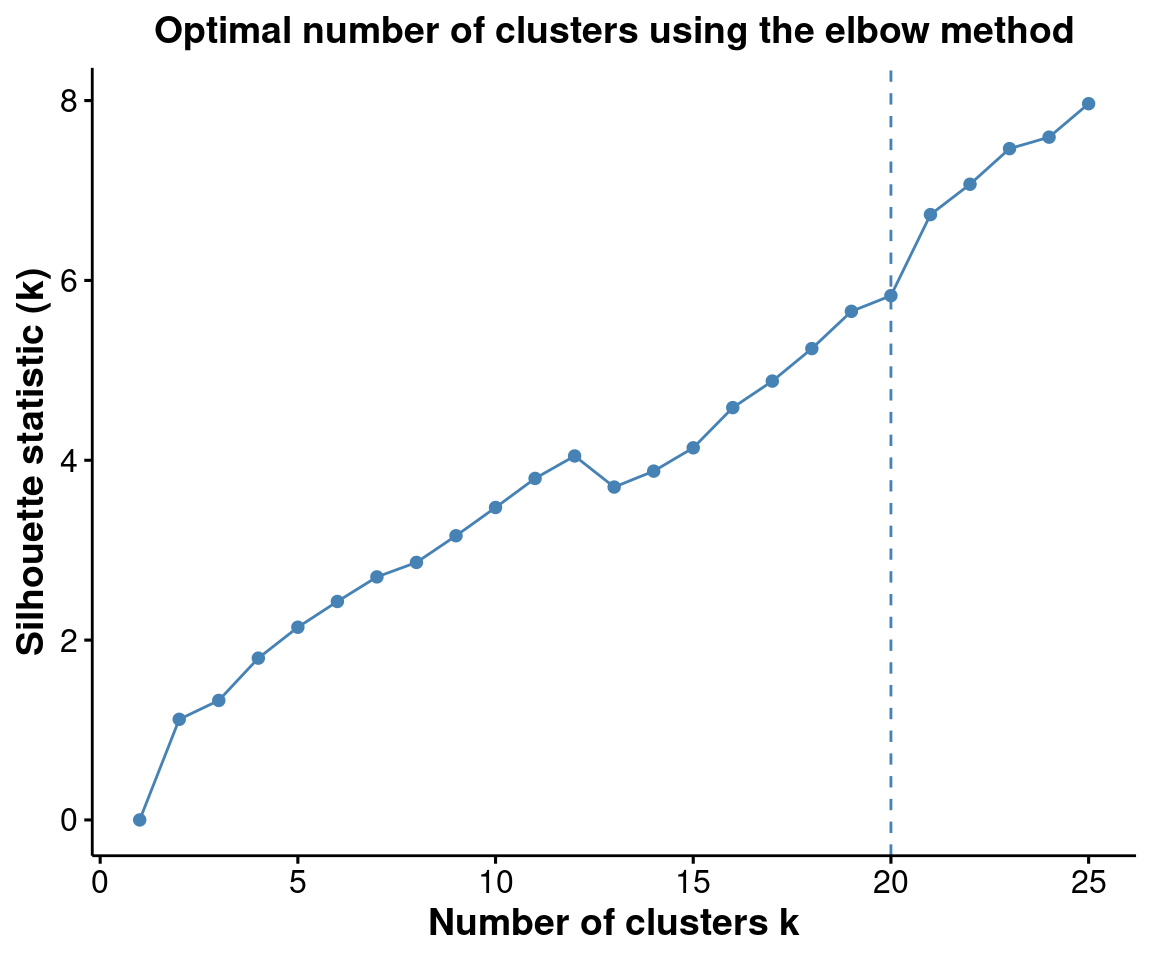
\includegraphics[keepaspectratio]{03-cell_annotation_files/figure-pdf/unnamed-chunk-12-5.png}}
\end{center}

Again, we see that the \texttt{Jump} statistics almost perfectly capture
the number of clusters. The \texttt{Gap} method is a close second with
\(15\) clusters. All the other methods significantly underestimates the
number of clusters.

\section{scClassify: Cell annotation}\label{scclassify-cell-annotation}

\section{Choosing between clustering and
annotation}\label{choosing-between-clustering-and-annotation}

\section{sessionInfo}\label{sessioninfo-2}

\begin{Shaded}
\begin{Highlighting}[]
\FunctionTok{sessionInfo}\NormalTok{()}
\end{Highlighting}
\end{Shaded}

\begin{verbatim}
R version 4.4.1 (2024-06-14)
Platform: x86_64-pc-linux-gnu
Running under: Debian GNU/Linux 12 (bookworm)

Matrix products: default
BLAS:   /usr/lib/x86_64-linux-gnu/openblas-pthread/libblas.so.3 
LAPACK: /usr/lib/x86_64-linux-gnu/openblas-pthread/libopenblasp-r0.3.21.so;  LAPACK version 3.11.0

locale:
 [1] LC_CTYPE=C.UTF-8       LC_NUMERIC=C           LC_TIME=C.UTF-8       
 [4] LC_COLLATE=C.UTF-8     LC_MONETARY=C.UTF-8    LC_MESSAGES=C.UTF-8   
 [7] LC_PAPER=C.UTF-8       LC_NAME=C              LC_ADDRESS=C          
[10] LC_TELEPHONE=C         LC_MEASUREMENT=C.UTF-8 LC_IDENTIFICATION=C   

time zone: Australia/Sydney
tzcode source: system (glibc)

attached base packages:
[1] stats4    stats     graphics  grDevices utils     datasets  methods  
[8] base     

other attached packages:
 [1] SingleCellExperiment_1.28.1 SummarizedExperiment_1.36.0
 [3] Biobase_2.66.0              GenomicRanges_1.58.0       
 [5] GenomeInfoDb_1.42.0         IRanges_2.40.0             
 [7] S4Vectors_0.44.0            BiocGenerics_0.52.0        
 [9] MatrixGenerics_1.18.0       matrixStats_1.4.1          
[11] FuseSOM_1.8.0              

loaded via a namespace (and not attached):
 [1] mnormt_2.1.1             permute_0.9-7            rlang_1.1.4             
 [4] magrittr_2.0.3           compiler_4.4.1           mgcv_1.9-1              
 [7] flexmix_2.3-19           analogue_0.17-7          vctrs_0.6.5             
[10] stringr_1.5.1            pkgconfig_2.0.3          crayon_1.5.3            
[13] fastmap_1.2.0            backports_1.5.0          magick_2.8.5            
[16] XVector_0.46.0           labeling_0.4.3           utf8_1.2.4              
[19] rmarkdown_2.29           UCSC.utils_1.2.0         tinytex_0.54            
[22] purrr_1.0.2              coop_0.6-3               xfun_0.49               
[25] modeltools_0.2-23        zlibbioc_1.52.0          jsonlite_1.8.9          
[28] DelayedArray_0.32.0      fpc_2.2-13               psych_2.4.6.26          
[31] broom_1.0.7              parallel_4.4.1           prabclus_2.3-4          
[34] cluster_2.1.6            R6_2.5.1                 profileModel_0.6.1      
[37] stringi_1.8.4            RColorBrewer_1.1-3       car_3.1-3               
[40] diptest_0.77-1           Rcpp_1.0.13-1            knitr_1.49              
[43] Matrix_1.7-1             splines_4.4.1            nnet_7.3-19             
[46] tidyselect_1.2.1         rstudioapi_0.17.1        abind_1.4-8             
[49] vegan_2.6-8              brglm_0.7.2              lattice_0.22-6          
[52] tibble_3.2.1             withr_3.0.2              evaluate_1.0.1          
[55] gridGraphics_0.5-1       proxy_0.4-27             kernlab_0.9-33          
[58] mclust_6.1.1             pillar_1.9.0             ggpubr_0.6.0            
[61] carData_3.0-5            generics_0.1.3           sp_2.1-4                
[64] ggplot2_3.5.1            munsell_0.5.1            scales_1.3.0            
[67] princurve_2.1.6          class_7.3-22             glue_1.8.0              
[70] pheatmap_1.0.12          tools_4.4.1              robustbase_0.99-4-1     
[73] ggsignif_0.6.4           fs_1.6.5                 fastcluster_1.2.6       
[76] grid_4.4.1               tidyr_1.3.1              colorspace_2.1-1        
[79] nlme_3.1-166             GenomeInfoDbData_1.2.13  Formula_1.2-5           
[82] cli_3.6.3                DataVisualizations_1.3.2 FCPS_1.3.4              
[85] fansi_1.0.6              S4Arrays_1.6.0           dplyr_1.1.4             
[88] DEoptimR_1.1-3           gtable_0.3.6             rstatix_0.7.2           
[91] yulab.utils_0.1.8        digest_0.6.37            SparseArray_1.6.0       
[94] ggplotify_0.1.2          farver_2.1.2             htmltools_0.5.8.1       
[97] lifecycle_1.0.4          httr_1.4.7               MASS_7.3-61             
\end{verbatim}

\bookmarksetup{startatroot}

\chapter{Cell localisation}\label{cell-localisation}

Now that we've finished performing all of our upstream preprocessing
(segmentation, quality control, and annotation), we can now begin
dissecting out interesting findings for our datasets. One of the primary
motivations behind pursuing a spatial technology as opposed to a
space-agnostic technology such as single-cell RNA sequencing, is that we
are more able to tease out whether changes are occurring spatially,
i.e.~are two cell types closer together in a disease state vs a
non-disease state. Whilst these changes are usually visually obvious, to
quantify localisation and dispersion relationships, more advanced
statistical modelling is required.

\begin{Shaded}
\begin{Highlighting}[]
\CommentTok{\# load required packages}
\FunctionTok{library}\NormalTok{(spicyR)}
\FunctionTok{library}\NormalTok{(Statial)}
\FunctionTok{library}\NormalTok{(ggplot2)}
\FunctionTok{library}\NormalTok{(SpatialExperiment)}
\FunctionTok{library}\NormalTok{(SpatialDatasets)}
\FunctionTok{library}\NormalTok{(imcRtools)}
\FunctionTok{library}\NormalTok{(dplyr)}
\FunctionTok{library}\NormalTok{(survival)}
\FunctionTok{library}\NormalTok{(tibble)}
\FunctionTok{library}\NormalTok{(treekoR)}
\FunctionTok{library}\NormalTok{(ggsurvfit)}

\NormalTok{nCores }\OtherTok{\textless{}{-}} \DecValTok{2}
\end{Highlighting}
\end{Shaded}

\section{spicyR: Cell localisation}\label{spicyr-cell-localisation}

This section provides step-by-step instructions on assessing how the
localisation of different cell types changes across different disease
conditions.

We use the (\textbf{keren2018?}) breast cancer dataset to compare the
spatial distribution of immune cells in individuals with different
levels of tumour infiltration (cold and compartmentalised).

The data is stored as a \texttt{SpatialExperiment} object and contains
single-cell spatial data from 41 images.

\begin{Shaded}
\begin{Highlighting}[]
\NormalTok{kerenSPE }\OtherTok{\textless{}{-}}\NormalTok{ SpatialDatasets}\SpecialCharTok{::}\FunctionTok{spe\_Keren\_2018}\NormalTok{()}
\end{Highlighting}
\end{Shaded}

The cell types in this dataset includes 11 immune cell types (double
negative CD3 T cells, CD4 T cells, B cells, monocytes, macrophages, CD8
T cells, neutrophils, natural killer cells, dendritic cells, regulatory
T cells), 2 structural cell types (endothelial, mesenchymal), 2 tumour
cell types (keratin+ tumour, tumour) and one unidentified category.
Below we've provided detailed information on the statistical backend of
\texttt{spicyR}.

\subsection{Linear modelling}\label{linear-modelling}

To investigate changes in localisation between two different cell types,
we measure the level of localisation between two cell types by modelling
with the L-function. The L-function is a variance-stabilised K-function
given by the equation

\[
\widehat{L_{ij}} (r) = \sqrt{\frac{\widehat{K_{ij}}(r)}{\pi}}
\]

with \(\widehat{K_{ij}}\) defined as

\[
\widehat{K_{ij}} (r) = \frac{|W|}{n_i n_j} \sum_{n_i} \sum_{n_j} 1 \{d_{ij} \leq r \} e_{ij} (r)
\]

where \(\widehat{K_{ij}}\) summarises the degree of co-localisation of
cell type \(j\) with cell type \(i\), \(n_i\) and \(n_j\) are the number
of cells of type \(i\) and \(j\), \(|W|\) is the image area, \(d_{ij}\)
is the distance between two cells and \(e_{ij} (r)\) is an edge
correcting factor.

Specifically, the mean difference between the experimental function and
the theoretical function is used as a measure for the level of
localisation, defined as

\[
u = \sum_{r' = r_{\text{min}}}^{r_{\text{max}}} \widehat L_{ij, \text{Experimental}} (r') - \widehat L_{ij, \text{Poisson}} (r')
\]

where \(u\) is the sum is taken over a discrete range of \(r\) between
\(r_{\text{min}}\) and \(r_{\text{max}}\). Differences of the statistic
\(u\) between two conditions is modelled using a weighted linear model.

\subsection{Test for changes in localisation for a specific pair of
cells}\label{test-for-changes-in-localisation-for-a-specific-pair-of-cells}

Firstly, we can test whether one cell type tends to be more localised
with another cell type in one condition compared to the other. This can
be done using the \texttt{spicy()} function, where we specify the
\texttt{condition} parameter.

In this example, we want to see whether or not neutrophils (\texttt{to})
tend to be found around CD8 T cells (\texttt{from}) in compartmentalised
tumours compared to cold tumours. Given that there are 3 conditions, we
can specify the desired conditions by setting the order of our
\texttt{condition} factor. \texttt{spicy} will choose the first level of
the factor as the base condition and the second level as the comparison
condition. \texttt{spicy} will also naturally coerce the
\texttt{condition} column into a factor if it is not already a factor.
The column containing cell type annotations can be specified using the
\texttt{cellTypeCol} argument. By default, \texttt{spicy} uses the
column named \texttt{cellType} in the \texttt{SpatialExperiment} object.

\begin{Shaded}
\begin{Highlighting}[]
\NormalTok{spicyTestPair }\OtherTok{\textless{}{-}} \FunctionTok{spicy}\NormalTok{(}
\NormalTok{  kerenSPE,}
  \AttributeTok{condition =} \StringTok{"tumour\_type"}\NormalTok{,}
  \AttributeTok{from =} \StringTok{"CD8\_T\_cell"}\NormalTok{,}
  \AttributeTok{to =} \StringTok{"Neutrophils"}
\NormalTok{)}

\FunctionTok{topPairs}\NormalTok{(spicyTestPair)}
\end{Highlighting}
\end{Shaded}

\begin{verbatim}
                        intercept coefficient      p.value   adj.pvalue
CD8_T_cell__Neutrophils  -109.081    112.0185 2.166646e-05 2.166646e-05
                              from          to
CD8_T_cell__Neutrophils CD8_T_cell Neutrophils
\end{verbatim}

We obtain a \texttt{spicy} object which details the results of the
modelling performed. The \texttt{topPairs()} function can be used to
obtain the associated coefficients and p-value.

As the \texttt{coefficient} in \texttt{spicyTestPair} is positive, we
find that neutrophils are significantly more likely to be found near CD8
T cells in the compartmentalised tumours group compared to the cold
tumour group.

\subsection{Test for changes in localisation for all pairwise cell
combinations}\label{test-for-changes-in-localisation-for-all-pairwise-cell-combinations}

We can perform what we did above for all pairwise combinations of cell
types by excluding the \texttt{from} and \texttt{to} parameters in
\texttt{spicy()}.

\begin{Shaded}
\begin{Highlighting}[]
\NormalTok{spicyTest }\OtherTok{\textless{}{-}} \FunctionTok{spicy}\NormalTok{(}
\NormalTok{  kerenSPE,}
  \AttributeTok{condition =} \StringTok{"tumour\_type"}
\NormalTok{)}

\FunctionTok{topPairs}\NormalTok{(spicyTest)}
\end{Highlighting}
\end{Shaded}

\begin{verbatim}
                            intercept coefficient      p.value   adj.pvalue
Macrophages__dn_T_CD3       56.446064   -50.08474 1.080273e-07 3.035568e-05
dn_T_CD3__Macrophages       54.987151   -48.38664 2.194018e-07 3.082595e-05
Macrophages__DC_or_Mono     73.239404   -59.90361 5.224660e-06 4.893765e-04
DC_or_Mono__Macrophages     71.777087   -58.46833 7.431172e-06 5.220399e-04
dn_T_CD3__dn_T_CD3         -63.786032   100.61010 2.878804e-05 1.208706e-03
Neutrophils__dn_T_CD3      -63.141840    69.64356 2.891872e-05 1.208706e-03
dn_T_CD3__Neutrophils      -63.133725    70.15508 3.011012e-05 1.208706e-03
DC__Macrophages             96.893239   -92.55112 1.801300e-04 5.758129e-03
Macrophages__DC             96.896215   -93.25194 1.844241e-04 5.758129e-03
CD4_T_cell__Keratin_Tumour  -4.845037   -22.14995 2.834659e-04 7.409016e-03
                                  from             to
Macrophages__dn_T_CD3      Macrophages       dn_T_CD3
dn_T_CD3__Macrophages         dn_T_CD3    Macrophages
Macrophages__DC_or_Mono    Macrophages     DC_or_Mono
DC_or_Mono__Macrophages     DC_or_Mono    Macrophages
dn_T_CD3__dn_T_CD3            dn_T_CD3       dn_T_CD3
Neutrophils__dn_T_CD3      Neutrophils       dn_T_CD3
dn_T_CD3__Neutrophils         dn_T_CD3    Neutrophils
DC__Macrophages                     DC    Macrophages
Macrophages__DC            Macrophages             DC
CD4_T_cell__Keratin_Tumour  CD4_T_cell Keratin_Tumour
\end{verbatim}

Again, we obtain a \texttt{spicy} object which outlines the result of
the linear models performed for each pairwise combination of cell types.

We can also examine the L-function metrics of individual images by using
the convenient \texttt{bind()} function on our \texttt{spicyTest}
results object.

\begin{Shaded}
\begin{Highlighting}[]
\FunctionTok{bind}\NormalTok{(spicyTest)[}\DecValTok{1}\SpecialCharTok{:}\DecValTok{5}\NormalTok{, }\DecValTok{1}\SpecialCharTok{:}\DecValTok{5}\NormalTok{]}
\end{Highlighting}
\end{Shaded}

\begin{verbatim}
  imageID         condition Keratin_Tumour__Keratin_Tumour
1       1             mixed                      -2.300602
2       2             mixed                      -1.989699
3       3 compartmentalised                      11.373530
4       4 compartmentalised                      33.931133
5       5 compartmentalised                      17.922818
  dn_T_CD3__Keratin_Tumour B_cell__Keratin_Tumour
1                -5.298543             -20.827279
2               -16.020022               3.025815
3               -21.857447             -24.962913
4               -36.438476             -40.470221
5               -20.816783             -38.138076
\end{verbatim}

The results can be represented as a bubble plot using the
\texttt{signifPlot()} function.

\begin{Shaded}
\begin{Highlighting}[]
\FunctionTok{signifPlot}\NormalTok{(}
\NormalTok{  spicyTest,}
  \AttributeTok{breaks =} \FunctionTok{c}\NormalTok{(}\SpecialCharTok{{-}}\DecValTok{3}\NormalTok{, }\DecValTok{3}\NormalTok{, }\DecValTok{1}\NormalTok{),}
  \AttributeTok{marksToPlot =} \FunctionTok{c}\NormalTok{(}\StringTok{"Macrophages"}\NormalTok{, }\StringTok{"DC\_or\_Mono"}\NormalTok{, }\StringTok{"dn\_T\_CD3"}\NormalTok{, }\StringTok{"Neutrophils"}\NormalTok{,}
                  \StringTok{"CD8\_T\_cell"}\NormalTok{, }\StringTok{"Keratin\_Tumour"}\NormalTok{)}
\NormalTok{)}
\end{Highlighting}
\end{Shaded}

\pandocbounded{\includegraphics[keepaspectratio]{04-cell_localisation_files/figure-pdf/unnamed-chunk-6-1.pdf}}

Here, we can observe that the most significant relationships occur
between macrophages and double negative CD3 T cells, suggesting that the
two cell types are far more dispersed in compartmentalised tumours
compared to cold tumours.

To examine a specific cell type-cell type relationship in more detail,
we can use \texttt{spicyBoxplot()} and specify either
\texttt{from\ =\ "Macrophages"} and \texttt{to\ =\ "dn\_T\_CD3"} or
\texttt{rank\ =\ 1}.

\begin{Shaded}
\begin{Highlighting}[]
\FunctionTok{spicyBoxPlot}\NormalTok{(}\AttributeTok{results =}\NormalTok{ spicyTest, }
             \CommentTok{\# from = "Macrophages",}
             \CommentTok{\# to = "dn\_T\_CD3"}
             \AttributeTok{rank =} \DecValTok{1}\NormalTok{)}
\end{Highlighting}
\end{Shaded}

\begin{verbatim}
Warning: Removed 2 rows containing non-finite outside the scale range
(`stat_boxplot()`).
\end{verbatim}

\pandocbounded{\includegraphics[keepaspectratio]{04-cell_localisation_files/figure-pdf/unnamed-chunk-7-1.pdf}}

\subsection{Linear modelling for custom
metrics}\label{linear-modelling-for-custom-metrics}

\texttt{spicyR} can also be applied to custom distance or abundance
metrics. A kNN interactions graph can be generated with the function
\texttt{buildSpatialGraph} from the \texttt{imcRtools} package. This
generates a \texttt{colPairs} object inside of the
\texttt{SpatialExperiment} object.

\texttt{spicyR} provides the function \texttt{convPairs} for converting
a \texttt{colPairs} object into an abundance matrix by calculating the
average number of nearby cells types for every cell type for a given
\texttt{k}. For example, if there exists on average 5 neutrophils for
every macrophage in image 1, the column
\texttt{Neutrophil\_\_Macrophage} would have a value of 5 for image 1.

\begin{Shaded}
\begin{Highlighting}[]
\NormalTok{kerenSPE }\OtherTok{\textless{}{-}}\NormalTok{ imcRtools}\SpecialCharTok{::}\FunctionTok{buildSpatialGraph}\NormalTok{(kerenSPE, }
                                         \AttributeTok{img\_id =} \StringTok{"imageID"}\NormalTok{, }
                                         \AttributeTok{type =} \StringTok{"knn"}\NormalTok{, }\AttributeTok{k =} \DecValTok{20}\NormalTok{,}
                                        \AttributeTok{coords =} \FunctionTok{c}\NormalTok{(}\StringTok{"x"}\NormalTok{, }\StringTok{"y"}\NormalTok{))}
\end{Highlighting}
\end{Shaded}

\begin{verbatim}
'sample_id's are duplicated across 'SpatialExperiment' objects to cbind; appending sample indices.
\end{verbatim}

\begin{verbatim}
The returned object is ordered by the 'imageID' entry.
\end{verbatim}

\begin{Shaded}
\begin{Highlighting}[]
\NormalTok{pairAbundances }\OtherTok{\textless{}{-}} \FunctionTok{convPairs}\NormalTok{(kerenSPE,}
                  \AttributeTok{colPair =} \StringTok{"knn\_interaction\_graph"}\NormalTok{)}

\FunctionTok{head}\NormalTok{(pairAbundances[}\StringTok{"B\_cell\_\_B\_cell"}\NormalTok{])}
\end{Highlighting}
\end{Shaded}

\begin{verbatim}
   B_cell__B_cell
1      12.7349608
10      0.2777778
11      0.0000000
12      1.3333333
13      1.2200957
14      0.0000000
\end{verbatim}

The custom distance or abundance metrics can then be included in the
analysis with the \texttt{alternateResult} parameter. The
\texttt{Statial} package contains other custom distance metrics which
can be used with \texttt{spicy}.

\begin{Shaded}
\begin{Highlighting}[]
\NormalTok{spicyTestColPairs }\OtherTok{\textless{}{-}} \FunctionTok{spicy}\NormalTok{(}
\NormalTok{  kerenSPE,}
  \AttributeTok{condition =} \StringTok{"tumour\_type"}\NormalTok{,}
  \AttributeTok{alternateResult =}\NormalTok{ pairAbundances,}
  \AttributeTok{weights =} \ConstantTok{FALSE}
\NormalTok{)}

\FunctionTok{topPairs}\NormalTok{(spicyTestColPairs)}
\end{Highlighting}
\end{Shaded}

\begin{verbatim}
                           intercept coefficient     p.value adj.pvalue
CD8_T_cell__Neutrophils  0.833333333  -0.7592968 0.002645466  0.3291833
B_cell__Tumour           0.001937984   0.2602822 0.004872664  0.3291833
Other_Immune__NK         0.012698413   0.2612881 0.005673068  0.3291833
Unidentified__CD8_T_cell 0.106626794   0.6387339 0.005906526  0.3291833
dn_T_CD3__NK             0.004242424   0.2148797 0.006317829  0.3291833
CD4_T_cell__Neutrophils  0.036213602   0.2947696 0.007902670  0.3291833
Tregs__CD4_T_cell        0.128876212   0.5726201 0.010207087  0.3291833
Endothelial__DC          0.008771930   0.3008523 0.011189533  0.3291833
Tumour__Neutrophils      0.021638939   0.2529045 0.011388850  0.3291833
Mesenchymal__Neutrophils 0.004504505   0.2494301 0.012761315  0.3291833
                                 from          to
CD8_T_cell__Neutrophils    CD8_T_cell Neutrophils
B_cell__Tumour                 B_cell      Tumour
Other_Immune__NK         Other_Immune          NK
Unidentified__CD8_T_cell Unidentified  CD8_T_cell
dn_T_CD3__NK                 dn_T_CD3          NK
CD4_T_cell__Neutrophils    CD4_T_cell Neutrophils
Tregs__CD4_T_cell               Tregs  CD4_T_cell
Endothelial__DC           Endothelial          DC
Tumour__Neutrophils            Tumour Neutrophils
Mesenchymal__Neutrophils  Mesenchymal Neutrophils
\end{verbatim}

\begin{Shaded}
\begin{Highlighting}[]
\FunctionTok{signifPlot}\NormalTok{(}
\NormalTok{  spicyTestColPairs,}
  \AttributeTok{breaks =} \FunctionTok{c}\NormalTok{(}\SpecialCharTok{{-}}\DecValTok{3}\NormalTok{, }\DecValTok{3}\NormalTok{, }\DecValTok{1}\NormalTok{),}
  \AttributeTok{marksToPlot =} \FunctionTok{c}\NormalTok{(}\StringTok{"Macrophages"}\NormalTok{, }\StringTok{"dn\_T\_CD3"}\NormalTok{, }\StringTok{"CD4\_T\_cell"}\NormalTok{, }
                  \StringTok{"B\_cell"}\NormalTok{, }\StringTok{"DC\_or\_Mono"}\NormalTok{, }\StringTok{"Neutrophils"}\NormalTok{, }\StringTok{"CD8\_T\_cell"}\NormalTok{)}
\NormalTok{)}
\end{Highlighting}
\end{Shaded}

\pandocbounded{\includegraphics[keepaspectratio]{04-cell_localisation_files/figure-pdf/unnamed-chunk-10-1.pdf}}

\subsection{Performing survival
analysis}\label{performing-survival-analysis}

\texttt{spicy} can also be used to perform survival analysis to asses
whether changes in co-localisation between cell types are associated
with survival probability. \texttt{spicy} requires the
\texttt{SingleCellExperiment} object being used to contain a column
called \texttt{survival} as a \texttt{Surv} object.

\begin{Shaded}
\begin{Highlighting}[]
\NormalTok{kerenSPE}\SpecialCharTok{$}\NormalTok{event }\OtherTok{=} \DecValTok{1} \SpecialCharTok{{-}}\NormalTok{ kerenSPE}\SpecialCharTok{$}\NormalTok{Censored}
\NormalTok{kerenSPE}\SpecialCharTok{$}\NormalTok{survival }\OtherTok{=} \FunctionTok{Surv}\NormalTok{(kerenSPE}\SpecialCharTok{$}\StringTok{\textasciigrave{}}\AttributeTok{Survival\_days\_capped*}\StringTok{\textasciigrave{}}\NormalTok{, kerenSPE}\SpecialCharTok{$}\NormalTok{event)}
\end{Highlighting}
\end{Shaded}

We can then perform survival analysis using the \texttt{spicy} function
by specifying \texttt{condition\ =\ "survival"}. We can then access the
corresponding coefficients and p-values by accessing the
\texttt{survivalResults} slot in the \texttt{spicy} results object.

\begin{Shaded}
\begin{Highlighting}[]
\CommentTok{\# Running survival analysis}
\NormalTok{spicySurvival }\OtherTok{=} \FunctionTok{spicy}\NormalTok{(kerenSPE,}
                      \AttributeTok{condition =} \StringTok{"survival"}\NormalTok{)}

\CommentTok{\# top 10 significant pairs}
\FunctionTok{head}\NormalTok{(spicySurvival}\SpecialCharTok{$}\NormalTok{survivalResults, }\DecValTok{10}\NormalTok{)}
\end{Highlighting}
\end{Shaded}

\begin{verbatim}
# A tibble: 10 x 4
   test                       coef se.coef    p.value
   <chr>                     <dbl>   <dbl>      <dbl>
 1 Other_Immune__Tregs     0.0236  0.00866 0.00000893
 2 CD4_T_cell__Tregs       0.0177  0.00685 0.0000124 
 3 Tregs__Other_Immune     0.0237  0.00873 0.0000126 
 4 Tregs__CD4_T_cell       0.0171  0.00676 0.0000285 
 5 CD8_T_cell__CD8_T_cell  0.00605 0.00272 0.000332  
 6 Tumour__CD8_T_cell     -0.0305  0.0114  0.000617  
 7 CD8_T_cell__Tumour     -0.0305  0.0116  0.000721  
 8 CD4_T_cell__dn_T_CD3    0.00845 0.00353 0.000794  
 9 dn_T_CD3__CD4_T_cell    0.00840 0.00353 0.000937  
10 DC__Other_Immune       -0.0289  0.0123  0.00103   
\end{verbatim}

\subsection{Accounting for tissue
inhomogeneity}\label{accounting-for-tissue-inhomogeneity}

The \texttt{spicy} function can also account for tissue inhomogeneity to
avoid false positives or negatives. This can be done by setting the
\texttt{sigma\ =} parameter within the spicy function. By default,
\texttt{sigma} is set to \texttt{NULL}, and \texttt{spicy} assumes a
homogeneous tissue structure.

For example, when we examine the L-function for
\texttt{Keratin\_Tumour\_\_Neutrophils} when \texttt{sigma\ =\ NULL} and
\texttt{Rs\ =\ 100}, the value is positive, indicating attraction
between the two cell types.

\begin{Shaded}
\begin{Highlighting}[]
\CommentTok{\# filter SPE object to obtain image 24 data}
\NormalTok{kerenSubset }\OtherTok{=}\NormalTok{ kerenSPE[, }\FunctionTok{colData}\NormalTok{(kerenSPE)}\SpecialCharTok{$}\NormalTok{imageID }\SpecialCharTok{==} \StringTok{"24"}\NormalTok{]}

\NormalTok{pairwiseAssoc }\OtherTok{=} \FunctionTok{getPairwise}\NormalTok{(kerenSubset, }
                            \AttributeTok{sigma =} \ConstantTok{NULL}\NormalTok{, }
                            \AttributeTok{Rs =} \DecValTok{100}\NormalTok{) }\SpecialCharTok{|\textgreater{}}
  \FunctionTok{as.data.frame}\NormalTok{()}

\NormalTok{pairwiseAssoc[[}\StringTok{"Keratin\_Tumour\_\_Neutrophils"}\NormalTok{]]}
\end{Highlighting}
\end{Shaded}

\begin{verbatim}
[1] 10.88892
\end{verbatim}

When we specify \texttt{sigma\ =\ 20} and re-calculate the L-function,
it indicates that there is no relationship between
\texttt{Keratin\_Tumour} and \texttt{Neutrophils}, i.e., there is no
major attraction or dispersion, as it now takes into account tissue
inhomogeneity.

\begin{Shaded}
\begin{Highlighting}[]
\NormalTok{pairwiseAssoc }\OtherTok{=} \FunctionTok{getPairwise}\NormalTok{(kerenSubset, }
                            \AttributeTok{sigma =} \DecValTok{20}\NormalTok{, }
                            \AttributeTok{Rs =} \DecValTok{100}\NormalTok{) }\SpecialCharTok{|\textgreater{}}
  \FunctionTok{as.data.frame}\NormalTok{()}

\NormalTok{pairwiseAssoc[[}\StringTok{"Keratin\_Tumour\_\_Neutrophils"}\NormalTok{]]}
\end{Highlighting}
\end{Shaded}

\begin{verbatim}
[1] 0.9024836
\end{verbatim}

\begin{Shaded}
\begin{Highlighting}[]
\CommentTok{\# obtain colData for image 24}
\NormalTok{cData }\OtherTok{=} \FunctionTok{colData}\NormalTok{(kerenSPE) }\SpecialCharTok{|\textgreater{}} \FunctionTok{as.data.frame}\NormalTok{() }\SpecialCharTok{|\textgreater{}} 
\NormalTok{          dplyr}\SpecialCharTok{::}\FunctionTok{filter}\NormalTok{(imageID }\SpecialCharTok{==} \StringTok{"24"}\NormalTok{)}

\CommentTok{\# obtain cells present in image 24}
\NormalTok{coords }\OtherTok{=} \FunctionTok{spatialCoords}\NormalTok{(kerenSPE) }\SpecialCharTok{|\textgreater{}} \FunctionTok{as.data.frame}\NormalTok{()}
\NormalTok{coords}\SpecialCharTok{$}\NormalTok{cellID }\OtherTok{=} \FunctionTok{rownames}\NormalTok{(coords)}
\NormalTok{coords }\OtherTok{=}\NormalTok{ coords }\SpecialCharTok{|\textgreater{}}\NormalTok{ dplyr}\SpecialCharTok{::}\FunctionTok{filter}\NormalTok{(cellID }\SpecialCharTok{\%in\%}\NormalTok{ cData}\SpecialCharTok{$}\NormalTok{CellID)}

\NormalTok{cData}\SpecialCharTok{$}\NormalTok{X }\OtherTok{=}\NormalTok{ coords}\SpecialCharTok{$}\NormalTok{x}
\NormalTok{cData}\SpecialCharTok{$}\NormalTok{Y }\OtherTok{=}\NormalTok{ coords}\SpecialCharTok{$}\NormalTok{y}

\NormalTok{cData }\OtherTok{=}\NormalTok{ cData }\SpecialCharTok{|\textgreater{}} 
\NormalTok{  dplyr}\SpecialCharTok{::}\FunctionTok{mutate}\NormalTok{(}\AttributeTok{cellTypeNew =} \FunctionTok{ifelse}\NormalTok{(cellType }\SpecialCharTok{\%in\%} \FunctionTok{c}\NormalTok{(}\StringTok{"Keratin\_Tumour"}\NormalTok{, }\StringTok{"Neutrophils"}\NormalTok{), }
\NormalTok{                                     cellType, }\StringTok{"Other"}\NormalTok{))}

\NormalTok{ pal }\OtherTok{=} \FunctionTok{setNames}\NormalTok{(}\FunctionTok{c}\NormalTok{(}\StringTok{"\#d6b11c"}\NormalTok{, }\StringTok{"\#850f07"}\NormalTok{), }
                \FunctionTok{c}\NormalTok{(}\StringTok{"Keratin\_Tumour"}\NormalTok{, }\StringTok{"Neutrophils"}\NormalTok{))}

\FunctionTok{ggplot}\NormalTok{() }\SpecialCharTok{+}
    \FunctionTok{stat\_density\_2d}\NormalTok{(}\AttributeTok{data =}\NormalTok{ cData, }\FunctionTok{aes}\NormalTok{(}\AttributeTok{x =}\NormalTok{ X, }\AttributeTok{y =}\NormalTok{ Y, }\AttributeTok{fill =} \FunctionTok{after\_stat}\NormalTok{(density)), }
                    \AttributeTok{geom =} \StringTok{"raster"}\NormalTok{, }
                    \AttributeTok{contour =} \ConstantTok{FALSE}\NormalTok{) }\SpecialCharTok{+}
    \FunctionTok{geom\_point}\NormalTok{(}\AttributeTok{data =}\NormalTok{ cData }\SpecialCharTok{|\textgreater{}} \FunctionTok{filter}\NormalTok{(cellType }\SpecialCharTok{!=} \StringTok{"Other"}\NormalTok{),}
               \FunctionTok{aes}\NormalTok{(}\AttributeTok{x =}\NormalTok{ X, }\AttributeTok{y =}\NormalTok{ Y, }\AttributeTok{colour =}\NormalTok{ cellTypeNew), }\AttributeTok{size =} \DecValTok{1}\NormalTok{) }\SpecialCharTok{+}
    \FunctionTok{scale\_color\_manual}\NormalTok{(}\AttributeTok{values =}\NormalTok{ pal) }\SpecialCharTok{+}
    \FunctionTok{scale\_fill\_distiller}\NormalTok{(}\AttributeTok{palette =} \StringTok{"Blues"}\NormalTok{, }\AttributeTok{direction =} \DecValTok{1}\NormalTok{) }\SpecialCharTok{+}
    \FunctionTok{theme\_classic}\NormalTok{() }\SpecialCharTok{+}
    \FunctionTok{labs}\NormalTok{(}\AttributeTok{title =} \StringTok{"image ID: 24"}\NormalTok{)}
\end{Highlighting}
\end{Shaded}

\pandocbounded{\includegraphics[keepaspectratio]{04-cell_localisation_files/figure-pdf/unnamed-chunk-15-1.pdf}}

Plotting image 24 shows that the supposed co-localisation occurs due to
the dense cluster of cells near the top of the image.

\subsection{Mixed effects modelling}\label{mixed-effects-modelling}

\texttt{spicyR} supports mixed effects modelling when multiple images
are obtained for each subject. In this case, \texttt{subject} is treated
as a random effect and \texttt{condition} is treated as a fixed effect.
To perform mixed effects modelling, we can specify the \texttt{subject}
parameter in the \texttt{spicy} function.

\begin{Shaded}
\begin{Highlighting}[]
\NormalTok{spicyMixedTest }\OtherTok{\textless{}{-}} \FunctionTok{spicy}\NormalTok{(}
\NormalTok{  diabetesData,}
  \AttributeTok{condition =} \StringTok{"stage"}\NormalTok{,}
  \AttributeTok{subject =} \StringTok{"case"}
\NormalTok{)}
\end{Highlighting}
\end{Shaded}

\section{Kontextual: Context aware cell
localisation}\label{kontextual-context-aware-cell-localisation}

\texttt{Kontextual} is a method for performing inference on cell
localisation which explicitly defines the contexts in which spatial
relationships between cells can be identified and interpreted. These
contexts may represent landmarks, spatial domains, or groups of
functionally similar cells which are consistent across regions. By
modelling spatial relationships between cells relative to these
contexts, \texttt{Kontextual} produces robust spatial quantifications
that are not confounded by biases such as the choice of region to image
and the tissue structure present in the images.

In this example we demonstrate how cell type hierarchies can be used as
a means to derive appropriate ``contexts'' for the evaluation of cell
localisation. We then demonstrate the types of conclusions which
\texttt{Kontextual} enables.

\subsection{Using cell type hierarchies to define a
``context''}\label{using-cell-type-hierarchies-to-define-a-context}

A cell type hierarchy may be used to define the ``context'' in which
cell type relationships are evaluated within. A cell type hierarchy
defines how cell types are functionally related to one another. The
bottom of the hierarchy represents homogeneous populations of a cell
type (child), the cell populations at the nodes of the hierarchy
represent broader parent populations with shared generalised function.
For example CD4 T cells may be considered a child population to the
Immune parent population.

There are two ways to define the cell type hierarchy. First, they can be
defined based on our biological understanding of the cell types. We can
represent this by creating a named list containing the names of each
parent and the associated vector of child cell types.

\emph{Note:} The \texttt{all} vector must be created to include cell
types which do not have a parent e.g.~the \emph{undefined} cell type in
this data set.

\begin{Shaded}
\begin{Highlighting}[]
\CommentTok{\# Examine all cell types in image}
\FunctionTok{unique}\NormalTok{(kerenSPE}\SpecialCharTok{$}\NormalTok{cellType)}
\end{Highlighting}
\end{Shaded}

\begin{verbatim}
 [1] "Keratin_Tumour" "dn_T_CD3"       "B_cell"         "CD4_T_cell"    
 [5] "DC_or_Mono"     "Unidentified"   "Macrophages"    "CD8_T_cell"    
 [9] "Other_Immune"   "Endothelial"    "Mono_or_Neu"    "Mesenchymal"   
[13] "Neutrophils"    "NK"             "Tumour"         "DC"            
[17] "Tregs"         
\end{verbatim}

\begin{Shaded}
\begin{Highlighting}[]
\CommentTok{\# Named list of parents and their child cell types}
\NormalTok{biologicalHierarchy }\OtherTok{=} \FunctionTok{list}\NormalTok{(}
  \StringTok{"tumour"} \OtherTok{=} \FunctionTok{c}\NormalTok{(}\StringTok{"Keratin\_Tumour"}\NormalTok{, }\StringTok{"Tumour"}\NormalTok{),}
  \StringTok{"tcells"} \OtherTok{=} \FunctionTok{c}\NormalTok{(}\StringTok{"dn\_T\_CD3"}\NormalTok{, }\StringTok{"CD4\_T\_cell"}\NormalTok{, }\StringTok{"CD8\_T\_cell"}\NormalTok{, }\StringTok{"Tregs"}\NormalTok{),}
  \StringTok{"myeloid"} \OtherTok{=} \FunctionTok{c}\NormalTok{(}\StringTok{"DC\_or\_Mono"}\NormalTok{, }\StringTok{"DC"}\NormalTok{, }\StringTok{"Mono\_or\_Neu"}\NormalTok{, }\StringTok{"Macrophages"}\NormalTok{, }\StringTok{"Neutrophils"}\NormalTok{),}
  \StringTok{"tissue"} \OtherTok{=} \FunctionTok{c}\NormalTok{(}\StringTok{"Endothelial"}\NormalTok{, }\StringTok{"Mesenchymal"}\NormalTok{)}
\NormalTok{)}

\CommentTok{\# Adding more broader immune parent populationse}
\NormalTok{biologicalHierarchy}\SpecialCharTok{$}\NormalTok{immune }\OtherTok{=} \FunctionTok{c}\NormalTok{(biologicalHierarchy}\SpecialCharTok{$}\NormalTok{bcells,}
\NormalTok{                               biologicalHierarchy}\SpecialCharTok{$}\NormalTok{tcells,}
\NormalTok{                               biologicalHierarchy}\SpecialCharTok{$}\NormalTok{myeloid,}
                               \StringTok{"NK"}\NormalTok{, }\StringTok{"Other\_Immune"}\NormalTok{, }\StringTok{"B\_cell"}\NormalTok{)}


\CommentTok{\# Creating a vector for all cellTypes}
\NormalTok{all }\OtherTok{\textless{}{-}} \FunctionTok{unique}\NormalTok{(kerenSPE}\SpecialCharTok{$}\NormalTok{cellType)}
\end{Highlighting}
\end{Shaded}

Alternatively, you can use the \texttt{treeKor} bioconductor package
\href{http://www.bioconductor.org/packages/release/bioc/html/treekoR.html}{treekoR}
to define these hierarchies in a data driven way.

\emph{Note:} These parent populations may not be accurate as we are
using a small subset of the data.

\begin{Shaded}
\begin{Highlighting}[]
\CommentTok{\# Calculate hierarchy using treekoR}
\NormalTok{kerenTree }\OtherTok{\textless{}{-}}\NormalTok{ treekoR}\SpecialCharTok{::}\FunctionTok{getClusterTree}\NormalTok{(}\FunctionTok{t}\NormalTok{(}\FunctionTok{assay}\NormalTok{(kerenSPE, }\StringTok{"intensities"}\NormalTok{)),}
\NormalTok{                            kerenSPE}\SpecialCharTok{$}\NormalTok{cellType,}
                            \AttributeTok{hierarchy\_method=}\StringTok{"hopach"}\NormalTok{,}
                            \AttributeTok{hopach\_K =} \DecValTok{1}\NormalTok{)}

\CommentTok{\# Convert treekoR result to a name list of parents and children.}
\NormalTok{treekorParents }\OtherTok{=} \FunctionTok{getParentPhylo}\NormalTok{(kerenTree)}

\NormalTok{treekorParents}
\end{Highlighting}
\end{Shaded}

\begin{verbatim}
$parent_1
 [1] "Keratin_Tumour" "DC_or_Mono"     "Unidentified"   "Macrophages"   
 [5] "Endothelial"    "Mono_or_Neu"    "Mesenchymal"    "Neutrophils"   
 [9] "Tumour"         "DC"            

$parent_2
[1] "dn_T_CD3"     "B_cell"       "CD4_T_cell"   "CD8_T_cell"   "Other_Immune"
[6] "NK"           "Tregs"       
\end{verbatim}

\subsection{Application on triple negative breast cancer
image.}\label{application-on-triple-negative-breast-cancer-image.}

Here we examine an image highlighted in the Keren et al.~2018 manuscript
where accounting for context information enables new conclusions. In
image 6 of the Keren et al.~dataset, we can see that \emph{p53+ tumour
cells} and \emph{immune cells} are dispersed i.e.~these two cell types
are not mixing. However we can also see that \emph{p53+ tumour cells}
appear much more localised to \emph{immune cells} relative to the tumour
context (\emph{tumour cells} and \emph{p53+ tumour cells}).

\begin{Shaded}
\begin{Highlighting}[]
\CommentTok{\# Lets define a new cell type vector}
\NormalTok{kerenSPE}\SpecialCharTok{$}\NormalTok{cellTypeNew }\OtherTok{\textless{}{-}}\NormalTok{ kerenSPE}\SpecialCharTok{$}\NormalTok{cellType}

\CommentTok{\# Select for all cells that express higher than baseline level of p53}
\NormalTok{p53Pos }\OtherTok{\textless{}{-}} \FunctionTok{assay}\NormalTok{(kerenSPE)[}\StringTok{"p53"}\NormalTok{, ] }\SpecialCharTok{\textgreater{}} \SpecialCharTok{{-}}\FloatTok{0.300460}

\CommentTok{\# Find p53+ tumour cells}
\NormalTok{kerenSPE}\SpecialCharTok{$}\NormalTok{cellTypeNew[kerenSPE}\SpecialCharTok{$}\NormalTok{cellType }\SpecialCharTok{\%in\%}\NormalTok{ biologicalHierarchy}\SpecialCharTok{$}\NormalTok{tumour] }\OtherTok{\textless{}{-}} \StringTok{"Tumour"}
\NormalTok{kerenSPE}\SpecialCharTok{$}\NormalTok{cellTypeNew[p53Pos }\SpecialCharTok{\&}\NormalTok{ kerenSPE}\SpecialCharTok{$}\NormalTok{cellType }\SpecialCharTok{\%in\%}\NormalTok{ biologicalHierarchy}\SpecialCharTok{$}\NormalTok{tumour] }\OtherTok{\textless{}{-}} \StringTok{"p53\_Tumour"}

\CommentTok{\# Group all immune cells under the name "Immune"}
\NormalTok{kerenSPE}\SpecialCharTok{$}\NormalTok{cellTypeNew[kerenSPE}\SpecialCharTok{$}\NormalTok{cellType }\SpecialCharTok{\%in\%}\NormalTok{ biologicalHierarchy}\SpecialCharTok{$}\NormalTok{immune] }\OtherTok{\textless{}{-}} \StringTok{"Immune"}

\NormalTok{kerenSPE}\SpecialCharTok{$}\NormalTok{x }\OtherTok{\textless{}{-}} \FunctionTok{spatialCoords}\NormalTok{(kerenSPE)[,}\StringTok{"x"}\NormalTok{]}
\NormalTok{kerenSPE}\SpecialCharTok{$}\NormalTok{y }\OtherTok{\textless{}{-}} \FunctionTok{spatialCoords}\NormalTok{(kerenSPE)[,}\StringTok{"y"}\NormalTok{]}

\CommentTok{\# Plot image 6}
\NormalTok{kerenSPE }\SpecialCharTok{|\textgreater{}}
  \FunctionTok{colData}\NormalTok{() }\SpecialCharTok{|\textgreater{}}
  \FunctionTok{as.data.frame}\NormalTok{() }\SpecialCharTok{|\textgreater{}}
  \FunctionTok{filter}\NormalTok{(imageID }\SpecialCharTok{==} \StringTok{"6"}\NormalTok{) }\SpecialCharTok{|\textgreater{}}
  \FunctionTok{filter}\NormalTok{(cellTypeNew }\SpecialCharTok{\%in\%} \FunctionTok{c}\NormalTok{(}\StringTok{"Immune"}\NormalTok{, }\StringTok{"Tumour"}\NormalTok{, }\StringTok{"p53\_Tumour"}\NormalTok{)) }\SpecialCharTok{|\textgreater{}}
  \FunctionTok{arrange}\NormalTok{(cellTypeNew) }\SpecialCharTok{|\textgreater{}}
  \FunctionTok{ggplot}\NormalTok{(}\FunctionTok{aes}\NormalTok{(}\AttributeTok{x =}\NormalTok{ x, }\AttributeTok{y =}\NormalTok{ y, }\AttributeTok{color =}\NormalTok{ cellTypeNew)) }\SpecialCharTok{+}
  \FunctionTok{geom\_point}\NormalTok{(}\AttributeTok{size =} \DecValTok{1}\NormalTok{) }\SpecialCharTok{+}
  \FunctionTok{scale\_colour\_manual}\NormalTok{(}\AttributeTok{values =} \FunctionTok{c}\NormalTok{(}\StringTok{"Immune"} \OtherTok{=} \StringTok{"\#505050"}\NormalTok{, }\StringTok{"p53\_Tumour"} \OtherTok{=} \StringTok{"\#64BC46"}\NormalTok{, }\StringTok{"Tumour"} \OtherTok{=} \StringTok{"\#D6D6D6"}\NormalTok{)) }\SpecialCharTok{+}
  \FunctionTok{guides}\NormalTok{(}\AttributeTok{colour =} \FunctionTok{guide\_legend}\NormalTok{(}\AttributeTok{title =} \StringTok{"Cell types"}\NormalTok{, }\AttributeTok{override.aes =} \FunctionTok{list}\NormalTok{(}\AttributeTok{size =} \DecValTok{3}\NormalTok{)))}
\end{Highlighting}
\end{Shaded}

\pandocbounded{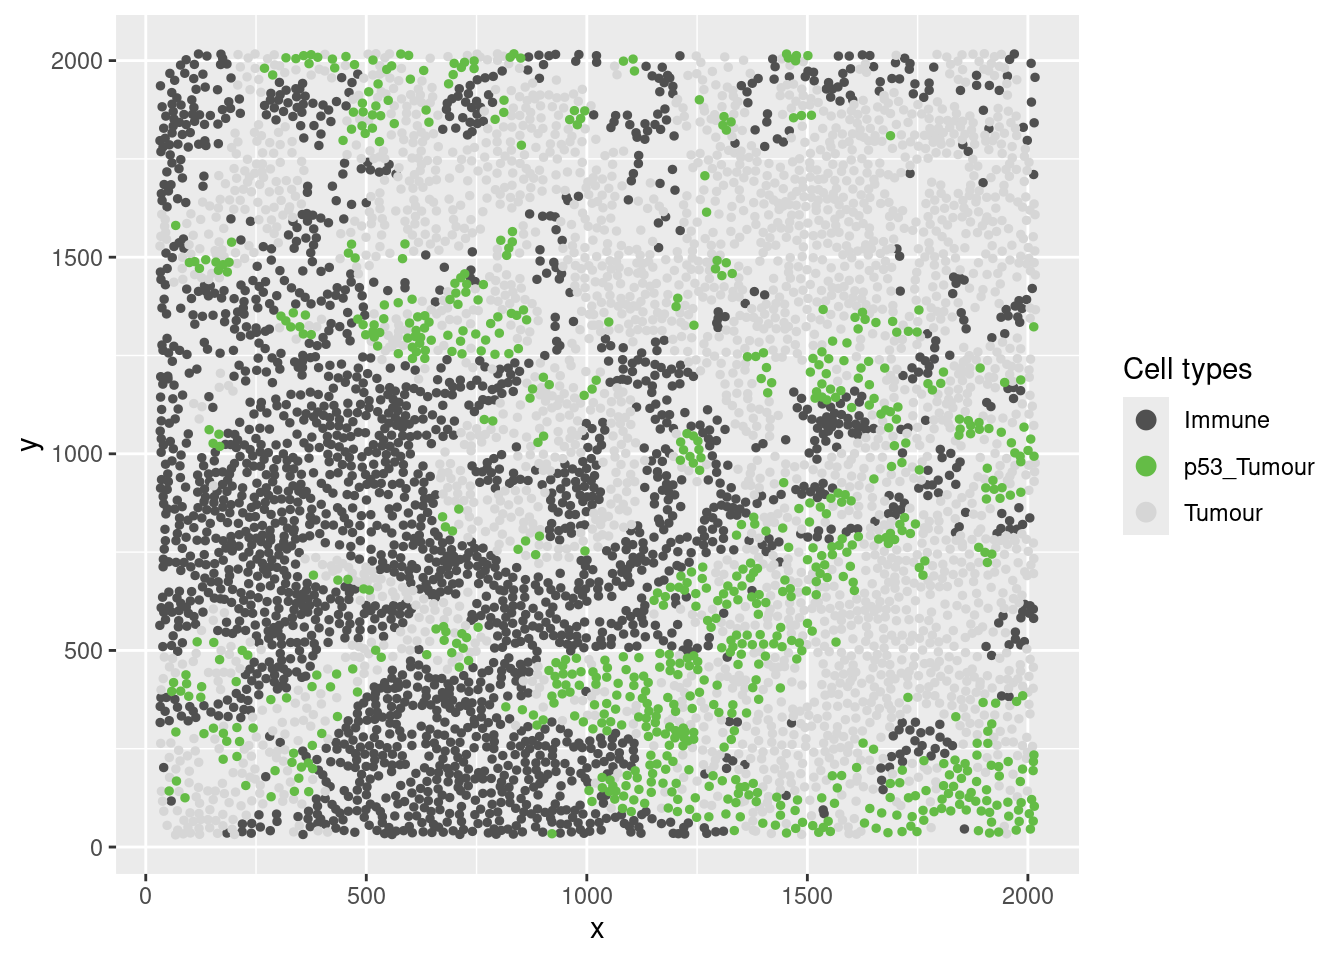
\includegraphics[keepaspectratio]{04-cell_localisation_files/figure-pdf/image6-1.pdf}}

\texttt{Kontextual} accepts a \texttt{SingleCellExperiment} object, a
single image, or list of images from a \texttt{SingleCellExperiment}
object, which gets passed into the \texttt{cells} argument. The two cell
types which will be evaluated are specified in the \texttt{to} and
\texttt{from} arguments. A parent population must also be specified in
the \texttt{parent} argument, note the parent cell population must
include the \texttt{to} cell type. The argument \texttt{r} will specify
the radius which the cell relationship will be evaluated on.
\texttt{Kontextual} supports parallel processing, the number of cores
can be specified using the \texttt{cores} argument. \texttt{Kontextual}
can take a single value or multiple values for each argument and will
test all combinations of the arguments specified.

We can calculate these relationships across all images for a single
radius (r = 100). Small radii will examine local spatial relationships,
whereas larger radii will examine global spatial relationships.

\begin{Shaded}
\begin{Highlighting}[]
\NormalTok{p53\_Kontextual }\OtherTok{\textless{}{-}} \FunctionTok{Kontextual}\NormalTok{(}
  \AttributeTok{cells =}\NormalTok{ kerenSPE,}
  \AttributeTok{r =} \DecValTok{100}\NormalTok{,}
  \AttributeTok{from =} \StringTok{"Immune"}\NormalTok{,}
  \AttributeTok{to =} \StringTok{"p53\_Tumour"}\NormalTok{,}
  \AttributeTok{parent =} \FunctionTok{c}\NormalTok{(}\StringTok{"p53\_Tumour"}\NormalTok{, }\StringTok{"Tumour"}\NormalTok{),}
  \AttributeTok{cellType =} \StringTok{"cellTypeNew"}
\NormalTok{)}

\NormalTok{p53\_Kontextual}
\end{Highlighting}
\end{Shaded}

\begin{verbatim}
   imageID               test   original  kontextual   r inhomL
1        1 Immune__p53_Tumour -16.212016  -1.6815952 100  FALSE
2       10 Immune__p53_Tumour -14.715356  -1.7937407 100  FALSE
3       11 Immune__p53_Tumour -11.696597  -7.4615661 100  FALSE
4       12 Immune__p53_Tumour  -9.777271  -2.6287005 100  FALSE
5       13 Immune__p53_Tumour -15.613023  -3.9937364 100  FALSE
6       14 Immune__p53_Tumour -14.671281  -4.2879138 100  FALSE
7       15 Immune__p53_Tumour   8.369183  10.6710168 100  FALSE
8       16 Immune__p53_Tumour -41.081088 -20.9688333 100  FALSE
9       17 Immune__p53_Tumour  -6.331105   5.0017104 100  FALSE
10      18 Immune__p53_Tumour  -1.953366   0.5795853 100  FALSE
11      19 Immune__p53_Tumour -27.834450 -18.7433000 100  FALSE
12       2 Immune__p53_Tumour  -4.989150  -0.5330373 100  FALSE
13      20 Immune__p53_Tumour -20.580091  -9.2542544 100  FALSE
14      21 Immune__p53_Tumour -14.300802  -7.1425133 100  FALSE
15      22 Immune__p53_Tumour -13.673007 -12.9663547 100  FALSE
16      23 Immune__p53_Tumour  15.803493  37.3584378 100  FALSE
17      24 Immune__p53_Tumour -30.319961 -31.8146274 100  FALSE
18      25 Immune__p53_Tumour   6.262995   6.9429103 100  FALSE
19      26 Immune__p53_Tumour -38.190137 -24.6000029 100  FALSE
20      27 Immune__p53_Tumour  -2.373587   4.4044397 100  FALSE
21      28 Immune__p53_Tumour -70.058615 -33.4395839 100  FALSE
22      29 Immune__p53_Tumour -20.728463  -7.0172785 100  FALSE
23       3 Immune__p53_Tumour   1.719549  44.5060581 100  FALSE
24      31 Immune__p53_Tumour -12.306957  -5.2820792 100  FALSE
25      32 Immune__p53_Tumour -18.174569 -10.8972277 100  FALSE
26      33 Immune__p53_Tumour -19.750457 -19.6246151 100  FALSE
27      34 Immune__p53_Tumour -49.004947 -35.1320255 100  FALSE
28      35 Immune__p53_Tumour -75.980619 -66.2395276 100  FALSE
29      36 Immune__p53_Tumour -18.853398 -21.4398044 100  FALSE
30      37 Immune__p53_Tumour -43.624905 -27.7162991 100  FALSE
31      38 Immune__p53_Tumour -12.544687  -3.0415484 100  FALSE
32      39 Immune__p53_Tumour -19.293290  -4.5192485 100  FALSE
33       4 Immune__p53_Tumour         NA          NA 100  FALSE
34      40 Immune__p53_Tumour -37.744261 -27.9604962 100  FALSE
35      41 Immune__p53_Tumour -33.776940 -22.6113096 100  FALSE
36       5 Immune__p53_Tumour         NA          NA 100  FALSE
37       6 Immune__p53_Tumour -24.897348  -1.2724241 100  FALSE
38       7 Immune__p53_Tumour -13.068307   0.6361875 100  FALSE
39       8 Immune__p53_Tumour         NA          NA 100  FALSE
40       9 Immune__p53_Tumour -31.857501   1.0261067 100  FALSE
\end{verbatim}

The \texttt{kontextCurve} function plots the L-function value and
Kontextual values over a range of radii. If the points lie above the red
line (expected pattern) then localisation is indicated for that radius,
if the points lie below the red line then dispersion is indicated.

As seen in the following plot the L-function produces negative values
over a range of radii, indicating that \emph{p53+ tumour cells} and
\emph{immune cells} are dispersed from one another. However by taking
into account the tumour context, \texttt{Kontextual} shows positive
values over some radii, indicating localisation between \emph{p53+
tumour cells} and \emph{immune cells}.

\begin{Shaded}
\begin{Highlighting}[]
\NormalTok{curves }\OtherTok{\textless{}{-}} \FunctionTok{kontextCurve}\NormalTok{(}
  \AttributeTok{cells =}\NormalTok{ kerenSPE,}
  \AttributeTok{from =} \StringTok{"Immune"}\NormalTok{,}
  \AttributeTok{to =} \StringTok{"p53\_Tumour"}\NormalTok{,}
  \AttributeTok{parent =} \FunctionTok{c}\NormalTok{(}\StringTok{"p53\_Tumour"}\NormalTok{, }\StringTok{"Tumour"}\NormalTok{),}
  \AttributeTok{rs =} \FunctionTok{seq}\NormalTok{(}\DecValTok{50}\NormalTok{, }\DecValTok{510}\NormalTok{, }\DecValTok{50}\NormalTok{),}
  \AttributeTok{image =} \StringTok{"6"}\NormalTok{,}
  \AttributeTok{cellType =} \StringTok{"cellTypeNew"}\NormalTok{,}
  \AttributeTok{cores =}\NormalTok{ nCores}
\NormalTok{)}

\FunctionTok{kontextPlot}\NormalTok{(curves)}
\end{Highlighting}
\end{Shaded}

\pandocbounded{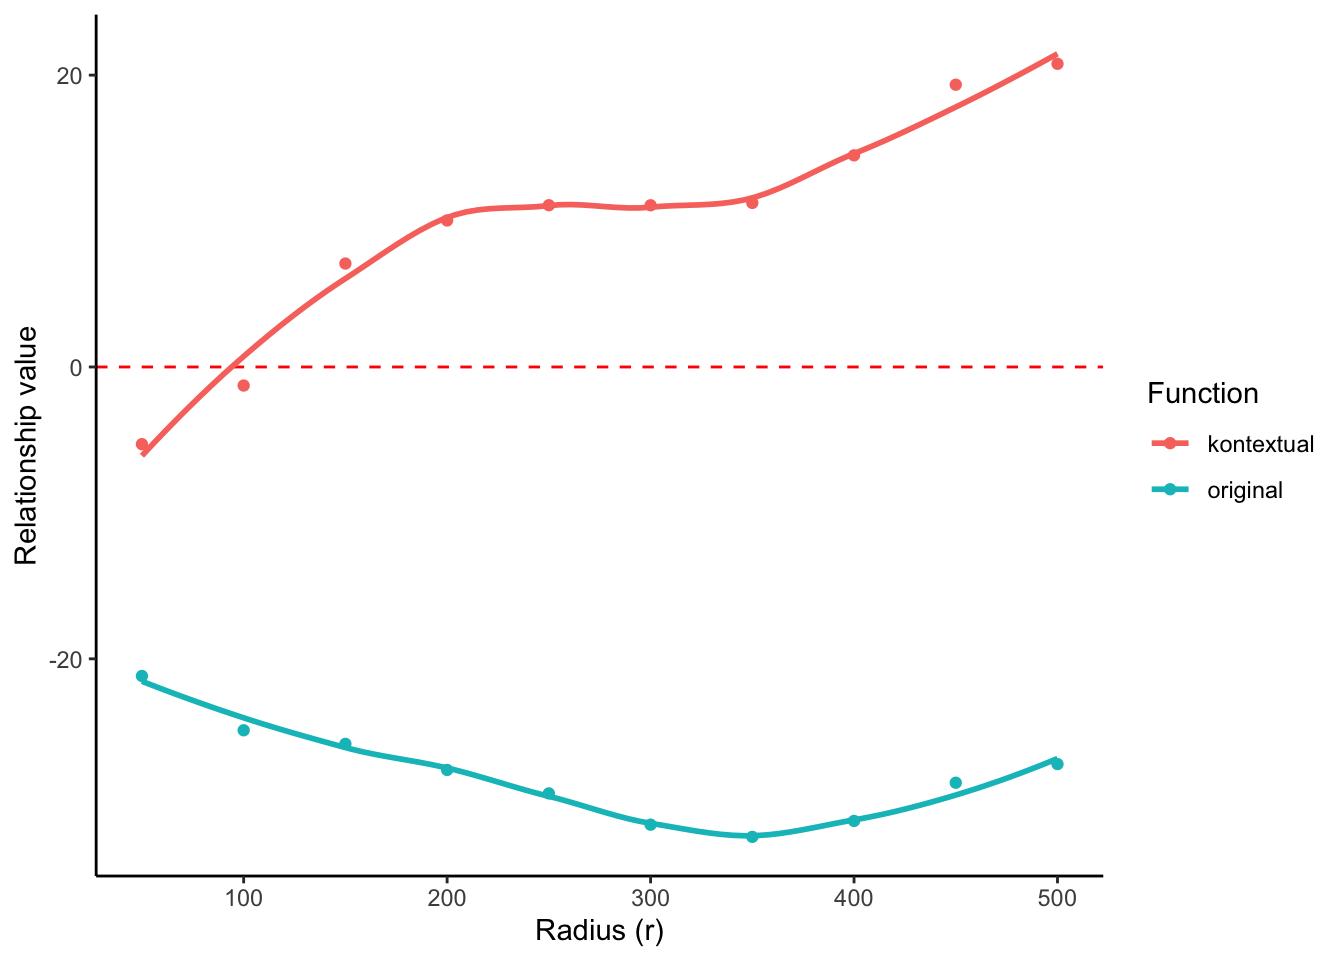
\includegraphics[keepaspectratio]{04-cell_localisation_files/figure-pdf/kontextCurve-1.pdf}}

Alternatively all pairwise cell relationships and their corresponding
parent in the dataset can be tested. A data frame with all pairwise
combinations can be creating using the \texttt{parentCombinations}
function. This function takes in a vector of all the cells, as well as
the named list of parents and children created earlier in the
\texttt{parentList} argument. As shown below the output is a data frame
specifying the \texttt{to}, \texttt{from}, and \texttt{parent} arguments
for \texttt{Kontextual}.

\emph{Note:} the output of \texttt{getPhyloParent} may also be using the
in the \texttt{parentList} argument, for example if you wanted to use
the treekoR defined hierarchy instead.

\begin{Shaded}
\begin{Highlighting}[]
\CommentTok{\# Get all relationships between cell types and their parents}
\NormalTok{parentDf }\OtherTok{\textless{}{-}} \FunctionTok{parentCombinations}\NormalTok{(}
  \AttributeTok{all =}\NormalTok{ all,}
  \AttributeTok{parentList =}\NormalTok{ biologicalHierarchy}
\NormalTok{)}
\end{Highlighting}
\end{Shaded}

\subsection{Calculating all pairwise
relationships}\label{calculating-all-pairwise-relationships}

Rather than specifying \texttt{to}, \texttt{from}, and \texttt{parent}
in \texttt{Kontextual}, the output from \texttt{parentCombinations} can
be inputed into \texttt{Kontextual} using the \texttt{parentDf}
argument, to examine all pairwise relationships in the dataset. This
chunk will take a significant amount of time to run, for demonstration
the results have been saved and are loaded in.

\begin{Shaded}
\begin{Highlighting}[]
\CommentTok{\# Running Kontextual on all relationships across all images.}
\NormalTok{kerenKontextual }\OtherTok{\textless{}{-}} \FunctionTok{Kontextual}\NormalTok{(}
  \AttributeTok{cells =}\NormalTok{ kerenSPE,}
  \AttributeTok{parentDf =}\NormalTok{ parentDf,}
  \AttributeTok{r =} \DecValTok{100}\NormalTok{,}
  \AttributeTok{cores =}\NormalTok{ nCores}
\NormalTok{)}
\end{Highlighting}
\end{Shaded}

For every pairwise relationship (named accordingly:
\texttt{from\_\_to\_\_parent}) \texttt{Kontextual} outputs the
L-function values (original) and the Kontextual value. The relationships
where the L-function and Kontextual disagree (e.g.~one metric is
positive and the other is negative) represent relationships where adding
context information results in different conclusions on the spatial
relationship between the two cell types.

\subsection{Associating the relationships with survival
outcomes.}\label{associating-the-relationships-with-survival-outcomes.}

To examine whether the features obtained from \texttt{Statial} are
associated with patient outcomes or groupings, we can use the
\texttt{spicy} function from the \texttt{spicyR} package.

In addition to this, the Kontextual results must be converted from a
\texttt{data.frame} to a wide \texttt{matrix}, this can be done using
\texttt{prepMatrix}. Note, to extract the original L-function values,
specify \texttt{column\ =\ "original"} in \texttt{prepMatrix}.

\begin{Shaded}
\begin{Highlighting}[]
\CommentTok{\# Converting Kontextual result into data matrix}
\NormalTok{kontextMat }\OtherTok{\textless{}{-}} \FunctionTok{prepMatrix}\NormalTok{(kerenKontextual)}

\CommentTok{\# Ensuring rownames of kontextMat match up with the image IDs of the SCE object}
\NormalTok{kontextMat }\OtherTok{\textless{}{-}}\NormalTok{ kontextMat[kerenSPE}\SpecialCharTok{$}\NormalTok{imageID }\SpecialCharTok{|\textgreater{}} \FunctionTok{unique}\NormalTok{(), ]}

\CommentTok{\# Replace NAs with 0}
\NormalTok{kontextMat[}\FunctionTok{is.na}\NormalTok{(kontextMat)] }\OtherTok{\textless{}{-}} \DecValTok{0}
\end{Highlighting}
\end{Shaded}

Finally, both the \texttt{SingleCellExperiment} object and the
Kontextual matrix are passed into the \texttt{spicy} function, with
\texttt{condition\ =\ "survival"}. The resulting coefficients and p
values can be obtained by accessing the \texttt{survivalResults} name.

\emph{Note:} You can specify additional covariates and include a subject
id for mixed effects survival modelling, see
\href{https://bioconductor.org/packages/release/bioc/html/spicyR.html}{spicyR}
for more information.

\begin{Shaded}
\begin{Highlighting}[]
\NormalTok{kerenSPE}\SpecialCharTok{$}\NormalTok{event }\OtherTok{=} \DecValTok{1} \SpecialCharTok{{-}}\NormalTok{ kerenSPE}\SpecialCharTok{$}\NormalTok{Censored}
\NormalTok{kerenSPE}\SpecialCharTok{$}\NormalTok{survival }\OtherTok{=} \FunctionTok{Surv}\NormalTok{(kerenSPE}\SpecialCharTok{$}\StringTok{\textasciigrave{}}\AttributeTok{Survival\_days\_capped*}\StringTok{\textasciigrave{}}\NormalTok{, kerenSPE}\SpecialCharTok{$}\NormalTok{event)}

\CommentTok{\# Running survival analysis}
\NormalTok{survivalResults }\OtherTok{=} \FunctionTok{spicy}\NormalTok{(}\AttributeTok{cells =}\NormalTok{ kerenSPE,}
                        \AttributeTok{alternateResult =}\NormalTok{ kontextMat,}
                        \AttributeTok{condition =} \StringTok{"survival"}\NormalTok{,}
                        \AttributeTok{weights =} \ConstantTok{TRUE}\NormalTok{)}

\FunctionTok{head}\NormalTok{(survivalResults}\SpecialCharTok{$}\NormalTok{survivalResults, }\DecValTok{10}\NormalTok{)}
\end{Highlighting}
\end{Shaded}

\begin{verbatim}
# A tibble: 10 x 4
   test                                    coef se.coef     p.value
   <chr>                                  <dbl>   <dbl>       <dbl>
 1 dn_T_CD3__Tregs__immune               0.0187 0.00716 0.000000572
 2 Other_Immune__Tregs__immune           0.0255 0.00885 0.000000727
 3 Tregs__dn_T_CD3__immune               0.0189 0.00715 0.00000169 
 4 Neutrophils__CD8_T_cell__immune       0.0178 0.00651 0.00000172 
 5 DC__dn_T_CD3__immune                 -0.0195 0.00661 0.00000710 
 6 DC__dn_T_CD3__tcells                 -0.0171 0.00758 0.0000167  
 7 Other_Immune__Keratin_Tumour__tumour  0.137  0.0406  0.0000212  
 8 CD4_T_cell__Tregs__immune             0.0216 0.00901 0.0000306  
 9 Other_Immune__DC__myeloid            -0.0181 0.00664 0.0000492  
10 Other_Immune__DC__immune             -0.0186 0.00669 0.0000656  
\end{verbatim}

The survival results can also be visualised using the
\texttt{signifPlot} function.

\begin{Shaded}
\begin{Highlighting}[]
\FunctionTok{signifPlot}\NormalTok{(survivalResults)}
\end{Highlighting}
\end{Shaded}

\pandocbounded{\includegraphics[keepaspectratio]{04-cell_localisation_files/figure-pdf/unnamed-chunk-21-1.pdf}}

As we can see from the results \texttt{DC\_\_NK\_\_immune} is the one of
the most significant pairwise relationship which contributes to patient
survival. That is the relationship between dendritic cells and natural
killer cells, relative to the parent population of immune cells. We can
see that there is a negative coefficient associated with this
relationship, which tells us an increase in localisation of these cell
types relative to immune cells leads to better survival outcomes for
patients.

The association between \texttt{DC\_\_NK\_\_immune} and survival can
also be visualised on a Kaplan-Meier curve. First, we extract survival
data from the \texttt{SingleCellExperiment} object and create a survival
vector.

\begin{Shaded}
\begin{Highlighting}[]
\CommentTok{\# Extracting survival data}
\NormalTok{survData }\OtherTok{\textless{}{-}}\NormalTok{ kerenSPE }\SpecialCharTok{|\textgreater{}}
  \FunctionTok{colData}\NormalTok{() }\SpecialCharTok{|\textgreater{}}
  \FunctionTok{data.frame}\NormalTok{() }\SpecialCharTok{|\textgreater{}}
  \FunctionTok{select}\NormalTok{(imageID, survival) }\SpecialCharTok{|\textgreater{}}
  \FunctionTok{unique}\NormalTok{()}

\CommentTok{\# Creating survival vector}
\NormalTok{kerenSurv }\OtherTok{\textless{}{-}}\NormalTok{ survData}\SpecialCharTok{$}\NormalTok{survival}
\FunctionTok{names}\NormalTok{(kerenSurv) }\OtherTok{\textless{}{-}}\NormalTok{ survData}\SpecialCharTok{$}\NormalTok{imageID}

\NormalTok{kerenSurv}
\end{Highlighting}
\end{Shaded}

\begin{verbatim}
    1     2     3     4     5     6     7     8     9    10    11    12    13 
 2612   745 3130+ 2523+ 1683+ 2275+   584   946 3767+ 3822+ 3774+ 4353+  1072 
   14    15    16    17    18    19    20    21    22    23    24    25    26 
4145+  1754   530  2842 5063+ 3725+ 4761+   635   NA?    91   194 4785+ 4430+ 
   27    28    29    31    32    33    34    35    36    37    38    39    40 
 3658 3767+  1319  1009 1568+ 1738+ 2832+ 2759+ 3063+ 2853+   NA? 2096+  3573 
   41 
3355+ 
\end{verbatim}

Next, we extract the Kontextual values of this relationship across all
images. We then determine if dendritic and natural killer cells are
relatively attracted or avoiding in each image by comparing the
Kontextual value in each image to the median Kontextual value.

Finally, we plot a Kaplan-Meier curve using the \texttt{ggsurvfit}
package. As shown below, when dendritic and natural killer cells are
more localised to one another relative to the immune cell population,
patients tend to have better survival outcomes.

\begin{Shaded}
\begin{Highlighting}[]
\CommentTok{\# Selecting most significant relationship}
\NormalTok{survRelationship }\OtherTok{\textless{}{-}}\NormalTok{ kontextMat[[}\StringTok{"DC\_\_NK\_\_immune"}\NormalTok{]]}
\NormalTok{survRelationship }\OtherTok{\textless{}{-}} \FunctionTok{ifelse}\NormalTok{(survRelationship }\SpecialCharTok{\textgreater{}} \FunctionTok{median}\NormalTok{(survRelationship), }\StringTok{"Localised"}\NormalTok{, }\StringTok{"Dispersed"}\NormalTok{)}

\CommentTok{\# Plotting Kaplan{-}Meier curve}
\FunctionTok{survfit2}\NormalTok{(kerenSurv }\SpecialCharTok{\textasciitilde{}}\NormalTok{ survRelationship) }\SpecialCharTok{|\textgreater{}}
  \FunctionTok{ggsurvfit}\NormalTok{() }\SpecialCharTok{+}
  \FunctionTok{ggtitle}\NormalTok{(}\StringTok{"DC\_\_NK\_\_immune"}\NormalTok{)}
\end{Highlighting}
\end{Shaded}

\pandocbounded{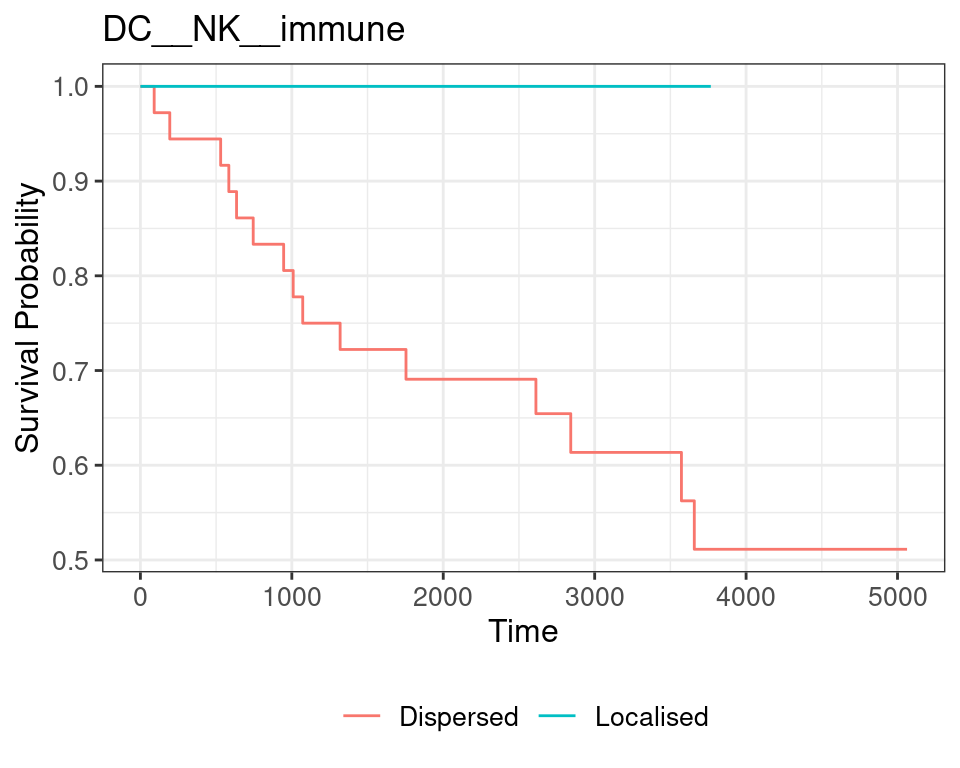
\includegraphics[keepaspectratio]{04-cell_localisation_files/figure-pdf/unnamed-chunk-23-1.pdf}}

\section{sessionInfo}\label{sessioninfo-3}

\begin{Shaded}
\begin{Highlighting}[]
\FunctionTok{sessionInfo}\NormalTok{()}
\end{Highlighting}
\end{Shaded}

\begin{verbatim}
R version 4.4.1 (2024-06-14)
Platform: x86_64-pc-linux-gnu
Running under: Debian GNU/Linux 12 (bookworm)

Matrix products: default
BLAS:   /usr/lib/x86_64-linux-gnu/openblas-pthread/libblas.so.3 
LAPACK: /usr/lib/x86_64-linux-gnu/openblas-pthread/libopenblasp-r0.3.21.so;  LAPACK version 3.11.0

locale:
 [1] LC_CTYPE=C.UTF-8       LC_NUMERIC=C           LC_TIME=C.UTF-8       
 [4] LC_COLLATE=C.UTF-8     LC_MONETARY=C.UTF-8    LC_MESSAGES=C.UTF-8   
 [7] LC_PAPER=C.UTF-8       LC_NAME=C              LC_ADDRESS=C          
[10] LC_TELEPHONE=C         LC_MEASUREMENT=C.UTF-8 LC_IDENTIFICATION=C   

time zone: Australia/Sydney
tzcode source: system (glibc)

attached base packages:
[1] stats4    stats     graphics  grDevices utils     datasets  methods  
[8] base     

other attached packages:
 [1] ggsurvfit_1.1.0             treekoR_1.14.0             
 [3] tibble_3.2.1                survival_3.7-0             
 [5] dplyr_1.1.4                 imcRtools_1.12.0           
 [7] SpatialDatasets_1.4.0       ExperimentHub_2.14.0       
 [9] AnnotationHub_3.14.0        BiocFileCache_2.14.0       
[11] dbplyr_2.5.0                SpatialExperiment_1.16.0   
[13] SingleCellExperiment_1.28.1 SummarizedExperiment_1.36.0
[15] Biobase_2.66.0              GenomicRanges_1.58.0       
[17] GenomeInfoDb_1.42.0         IRanges_2.40.0             
[19] S4Vectors_0.44.0            BiocGenerics_0.52.0        
[21] MatrixGenerics_1.18.0       matrixStats_1.4.1          
[23] ggplot2_3.5.1               Statial_1.8.0              
[25] spicyR_1.18.0              

loaded via a namespace (and not attached):
  [1] vroom_1.6.5                 tiff_0.1-12                
  [3] goftest_1.2-3               DT_0.33                    
  [5] Biostrings_2.74.0           HDF5Array_1.34.0           
  [7] TH.data_1.1-2               vctrs_0.6.5                
  [9] spatstat.random_3.3-2       digest_0.6.37              
 [11] png_0.1-8                   shape_1.4.6.1              
 [13] proxy_0.4-27                ggrepel_0.9.6              
 [15] deldir_2.0-4                magick_2.8.5               
 [17] MASS_7.3-61                 reshape2_1.4.4             
 [19] httpuv_1.6.15               foreach_1.5.2              
 [21] withr_3.0.2                 ggfun_0.1.7                
 [23] xfun_0.49                   ggpubr_0.6.0               
 [25] memoise_2.0.1               RTriangle_1.6-0.14         
 [27] cytomapper_1.18.0           ggbeeswarm_0.7.2           
 [29] RProtoBufLib_2.18.0         systemfonts_1.1.0          
 [31] tidytree_0.4.6              zoo_1.8-12                 
 [33] GlobalOptions_0.1.2         Formula_1.2-5              
 [35] KEGGREST_1.46.0             promises_1.3.0             
 [37] httr_1.4.7                  rstatix_0.7.2              
 [39] rhdf5filters_1.18.0         rhdf5_2.50.0               
 [41] rstudioapi_0.17.1           UCSC.utils_1.2.0           
 [43] units_0.8-5                 generics_0.1.3             
 [45] concaveman_1.1.0            curl_6.0.1                 
 [47] zlibbioc_1.52.0             ggraph_2.2.1               
 [49] polyclip_1.10-7             GenomeInfoDbData_1.2.13    
 [51] SparseArray_1.6.0           fftwtools_0.9-11           
 [53] xtable_1.8-4                stringr_1.5.1              
 [55] doParallel_1.0.17           evaluate_1.0.1             
 [57] S4Arrays_1.6.0              hms_1.1.3                  
 [59] colorspace_2.1-1            filelock_1.0.3             
 [61] spatstat.data_3.1-2         magrittr_2.0.3             
 [63] readr_2.1.5                 later_1.3.2                
 [65] viridis_0.6.5               ggtree_3.14.0              
 [67] lattice_0.22-6              spatstat.geom_3.3-3        
 [69] XML_3.99-0.17               scuttle_1.16.0             
 [71] ggupset_0.4.0               class_7.3-22               
 [73] svgPanZoom_0.3.4            pillar_1.9.0               
 [75] nlme_3.1-166                iterators_1.0.14           
 [77] EBImage_4.48.0              compiler_4.4.1             
 [79] beachmat_2.22.0             stringi_1.8.4              
 [81] sf_1.0-19                   tensor_1.5                 
 [83] minqa_1.2.8                 ClassifyR_3.10.0           
 [85] plyr_1.8.9                  crayon_1.5.3               
 [87] abind_1.4-8                 gridGraphics_0.5-1         
 [89] locfit_1.5-9.10             sp_2.1-4                   
 [91] graphlayouts_1.2.0          bit_4.5.0                  
 [93] terra_1.7-83                sandwich_3.1-1             
 [95] codetools_0.2-20            multcomp_1.4-26            
 [97] e1071_1.7-16                GetoptLong_1.0.5           
 [99] plotly_4.10.4               mime_0.12                  
[101] MultiAssayExperiment_1.32.0 splines_4.4.1              
[103] circlize_0.4.16             Rcpp_1.0.13-1              
[105] knitr_1.49                  blob_1.2.4                 
[107] utf8_1.2.4                  clue_0.3-66                
[109] BiocVersion_3.20.0          lme4_1.1-35.5              
[111] fs_1.6.5                    nnls_1.6                   
[113] ggplotify_0.1.2             ggsignif_0.6.4             
[115] Matrix_1.7-1                scam_1.2-17                
[117] statmod_1.5.0               tzdb_0.4.0                 
[119] svglite_2.1.3               tweenr_2.0.3               
[121] pkgconfig_2.0.3             pheatmap_1.0.12            
[123] tools_4.4.1                 cachem_1.1.0               
[125] RSQLite_2.3.7               viridisLite_0.4.2          
[127] DBI_1.2.3                   numDeriv_2016.8-1.1        
[129] fastmap_1.2.0               rmarkdown_2.29             
[131] scales_1.3.0                grid_4.4.1                 
[133] shinydashboard_0.7.2        broom_1.0.7                
[135] patchwork_1.3.0             BiocManager_1.30.25        
[137] carData_3.0-5               farver_2.1.2               
[139] tidygraph_1.3.1             mgcv_1.9-1                 
[141] yaml_2.3.10                 ggthemes_5.1.0             
[143] cli_3.6.3                   purrr_1.0.2                
[145] hopach_2.66.0               lifecycle_1.0.4            
[147] mvtnorm_1.3-2               backports_1.5.0            
[149] BiocParallel_1.40.0         cytolib_2.18.0             
[151] gtable_0.3.6                rjson_0.2.23               
[153] parallel_4.4.1              ape_5.8                    
[155] limma_3.62.1                jsonlite_1.8.9             
[157] edgeR_4.4.0                 bitops_1.0-9               
[159] bit64_4.5.2                 Rtsne_0.17                 
[161] FlowSOM_2.14.0              yulab.utils_0.1.8          
[163] spatstat.utils_3.1-1        BiocNeighbors_2.0.0        
[165] ranger_0.17.0               flowCore_2.18.0            
[167] bdsmatrix_1.3-7             spatstat.univar_3.1-1      
[169] lazyeval_0.2.2              shiny_1.9.1                
[171] ConsensusClusterPlus_1.70.0 htmltools_0.5.8.1          
[173] diffcyt_1.26.0              rappdirs_0.3.3             
[175] tinytex_0.54                distances_0.1.11           
[177] glue_1.8.0                  XVector_0.46.0             
[179] RCurl_1.98-1.16             treeio_1.30.0              
[181] classInt_0.4-10             coxme_2.2-22               
[183] jpeg_0.1-10                 gridExtra_2.3              
[185] boot_1.3-31                 igraph_2.1.1               
[187] R6_2.5.1                    tidyr_1.3.1                
[189] ggiraph_0.8.10              labeling_0.4.3             
[191] ggh4x_0.2.8                 cluster_2.1.6              
[193] Rhdf5lib_1.28.0             aplot_0.2.3                
[195] nloptr_2.1.1                DelayedArray_0.32.0        
[197] tidyselect_1.2.1            vipor_0.4.7                
[199] ggforce_0.4.2               raster_3.6-30              
[201] car_3.1-3                   AnnotationDbi_1.68.0       
[203] munsell_0.5.1               KernSmooth_2.23-24         
[205] data.table_1.16.2           htmlwidgets_1.6.4          
[207] ComplexHeatmap_2.22.0       RColorBrewer_1.1-3         
[209] rlang_1.1.4                 spatstat.sparse_3.1-0      
[211] spatstat.explore_3.3-3      lmerTest_3.1-3             
[213] uuid_1.2-1                  colorRamps_2.3.4           
[215] ggnewscale_0.5.0            fansi_1.0.6                
[217] beeswarm_0.4.0             
\end{verbatim}

\bookmarksetup{startatroot}

\chapter{Spatial domains}\label{spatial-domains}

\section{Why look at spatial
domains?}\label{why-look-at-spatial-domains}

Beyond spatial relationships between cell types, imaging datasets also
contain another source of rich information - spatial domains. To give an
idea of what spatial domains might visually look like, we've provided an
image on the right, where we can clearly map out our healthy epithelial
tissue spatial domain on the left of the image, and our immune and
tumour domains on the right of the image.

However, spatial domains tend to be highly dependent on the biological
question being answered. For example, when your primary tissue of
interest are solid tumours, spatial domain analysis can provide insights
into proportion of tumour domain vs immune domains, or how tumour
domains differ between progressive and non-progressive cancers.
Alternatively, if your primary tissue of interest is diabetes, spatial
domains can provide insights into marker or cell type differences in
your pancreatic islets.

In this section, we'll be exploring the use of \texttt{lisaClust} on two
different datasets to help inform

\begin{Shaded}
\begin{Highlighting}[]
\CommentTok{\# load required packages}
\FunctionTok{library}\NormalTok{(lisaClust)}
\FunctionTok{library}\NormalTok{(spicyR)}
\FunctionTok{library}\NormalTok{(ggplot2)}
\FunctionTok{library}\NormalTok{(SingleCellExperiment)}
\FunctionTok{library}\NormalTok{(SpatialDatasets)}
\end{Highlighting}
\end{Shaded}

\section{lisaClust}\label{lisaclust-1}

Clustering local indicators of spatial association (LISA) functions is a
methodology for identifying consistent spatial organisation of multiple
cell-types in an unsupervised way. This can be used to enable the
characterization of interactions between multiple cell-types
simultaneously and can complement traditional pairwise analysis. In our
implementation our LISA curves are a localised summary of an L-function
from a Poisson point process model. Our framework \texttt{lisaClust} can
be used to provide a high-level summary of cell-type colocalization in
high-parameter spatial cytometry data, facilitating the identification
of distinct tissue compartments or identification of complex cellular
microenvironments.

\subsection{How lisaClust works}\label{how-lisaclust-works}

The workflow that lisaClust uses to identify regions of tissue with
similar localisation patterns of cells contains multiple key steps.
First, cells are treated as objects and assigned coordinates in an x-y
space. Second, distances between all cells are calculated and then, by
modeling the cells as a multi-type Poisson point process, the distances
are used to calculate local indicators of spatial association (LISA).
These LISA curves summarize the spatial association between each cell
and a specific cell type over a range of radii, r. The LISA curves are
calculated for each cell and cell type and then clustered to assign a
region label for each cell.

\subsection{Case study: Keren}\label{case-study-keren}

We will start by reading in the data from the \texttt{SpatialDatasets}
package as a \texttt{SingleCellExperiment} object. Here the data is in a
format consistent with that outputted by CellProfiler.

\begin{Shaded}
\begin{Highlighting}[]
\NormalTok{kerenSPE }\OtherTok{\textless{}{-}}\NormalTok{ SpatialDatasets}\SpecialCharTok{::}\FunctionTok{spe\_Keren\_2018}\NormalTok{()}
\end{Highlighting}
\end{Shaded}

\begin{verbatim}
see ?SpatialDatasets and browseVignettes('SpatialDatasets') for documentation
\end{verbatim}

\begin{verbatim}
loading from cache
\end{verbatim}

\subsubsection{Generate LISA curves}\label{generate-lisa-curves}

This data includes annotation of the cell-types of each cell. Hence, we
can move directly to performing k-means clustering on the local
indicators of spatial association (LISA) functions using the
\texttt{lisaClust} function, remembering to specify the
\texttt{imageID}, \texttt{cellType}, and \texttt{spatialCoords} columns
in \texttt{colData}. For the purpose of demonstration, we will be using
only images 5 and 6 of the \texttt{kerenSPE} dataset.

\begin{Shaded}
\begin{Highlighting}[]
\NormalTok{kerenSPE }\OtherTok{\textless{}{-}}\NormalTok{ kerenSPE[,kerenSPE}\SpecialCharTok{$}\NormalTok{imageID }\SpecialCharTok{\%in\%} \FunctionTok{c}\NormalTok{(}\StringTok{"5"}\NormalTok{, }\StringTok{"6"}\NormalTok{)]}

\NormalTok{kerenSPE }\OtherTok{\textless{}{-}} \FunctionTok{lisaClust}\NormalTok{(kerenSPE,}
  \AttributeTok{k =} \DecValTok{5}
\NormalTok{)}
\end{Highlighting}
\end{Shaded}

\begin{verbatim}
Generating local L-curves.
\end{verbatim}

These regions are stored in \texttt{colData} and can be extracted.

\begin{Shaded}
\begin{Highlighting}[]
\FunctionTok{colData}\NormalTok{(kerenSPE)[, }\FunctionTok{c}\NormalTok{(}\StringTok{"imageID"}\NormalTok{, }\StringTok{"region"}\NormalTok{)] }\SpecialCharTok{|\textgreater{}}
  \FunctionTok{head}\NormalTok{(}\DecValTok{20}\NormalTok{)}
\end{Highlighting}
\end{Shaded}

\begin{verbatim}
DataFrame with 20 rows and 2 columns
          imageID      region
      <character> <character>
21154           5    region_5
21155           5    region_5
21156           5    region_5
21157           5    region_2
21158           5    region_2
...           ...         ...
21169           5    region_2
21170           5    region_2
21171           5    region_3
21172           5    region_2
21173           5    region_3
\end{verbatim}

\subsubsection{Examine cell type
enrichment}\label{examine-cell-type-enrichment}

\texttt{lisaClust} also provides a convenient function,
\texttt{regionMap}, for examining which cell types are located in which
regions. In this example, we use this to check which cell types appear
more frequently in each region than expected by chance.

Here, we clearly see that healthy epithelial and mesenchymal tissue are
highly concentrated in region 1, immune cells are concentrated in
regions 2 and 4, whilst tumour cells are concentrated in region 3.

We can further segregate these cells by increasing the number of
clusters, i.e., increasing the parameter \texttt{k\ =} in the
\texttt{lisaClust()} function. For the purposes of demonstration, let's
take a look at the \texttt{hatchingPlot} of these regions.

\begin{Shaded}
\begin{Highlighting}[]
\FunctionTok{regionMap}\NormalTok{(kerenSPE,}
  \AttributeTok{type =} \StringTok{"bubble"}
\NormalTok{)}
\end{Highlighting}
\end{Shaded}

\pandocbounded{\includegraphics[keepaspectratio]{05-cellular_niches_files/figure-pdf/unnamed-chunk-5-1.pdf}}

\subsubsection{Plot identified regions}\label{plot-identified-regions}

Finally, we can use \texttt{hatchingPlot} to construct a \texttt{ggplot}
object where the regions are marked by different hatching patterns. This
allows us to visualize the 5 regions and 17 cell-types simultaneously.

\begin{Shaded}
\begin{Highlighting}[]
\FunctionTok{hatchingPlot}\NormalTok{(kerenSPE, }\AttributeTok{nbp =} \DecValTok{300}\NormalTok{)}
\end{Highlighting}
\end{Shaded}

\begin{verbatim}
Concave windows are temperamental. Try choosing values of window.length > and < 1 if you have problems.
\end{verbatim}

\pandocbounded{\includegraphics[keepaspectratio]{05-cellular_niches_files/figure-pdf/unnamed-chunk-6-1.pdf}}

\section{sessionInfo}\label{sessioninfo-4}

\begin{Shaded}
\begin{Highlighting}[]
\FunctionTok{sessionInfo}\NormalTok{()}
\end{Highlighting}
\end{Shaded}

\begin{verbatim}
R version 4.4.1 (2024-06-14)
Platform: x86_64-pc-linux-gnu
Running under: Debian GNU/Linux 12 (bookworm)

Matrix products: default
BLAS:   /usr/lib/x86_64-linux-gnu/openblas-pthread/libblas.so.3 
LAPACK: /usr/lib/x86_64-linux-gnu/openblas-pthread/libopenblasp-r0.3.21.so;  LAPACK version 3.11.0

locale:
 [1] LC_CTYPE=C.UTF-8       LC_NUMERIC=C           LC_TIME=C.UTF-8       
 [4] LC_COLLATE=C.UTF-8     LC_MONETARY=C.UTF-8    LC_MESSAGES=C.UTF-8   
 [7] LC_PAPER=C.UTF-8       LC_NAME=C              LC_ADDRESS=C          
[10] LC_TELEPHONE=C         LC_MEASUREMENT=C.UTF-8 LC_IDENTIFICATION=C   

time zone: Australia/Sydney
tzcode source: system (glibc)

attached base packages:
[1] stats4    stats     graphics  grDevices utils     datasets  methods  
[8] base     

other attached packages:
 [1] SpatialDatasets_1.4.0       SpatialExperiment_1.16.0   
 [3] ExperimentHub_2.14.0        AnnotationHub_3.14.0       
 [5] BiocFileCache_2.14.0        dbplyr_2.5.0               
 [7] SingleCellExperiment_1.28.1 SummarizedExperiment_1.36.0
 [9] Biobase_2.66.0              GenomicRanges_1.58.0       
[11] GenomeInfoDb_1.42.0         IRanges_2.40.0             
[13] S4Vectors_0.44.0            BiocGenerics_0.52.0        
[15] MatrixGenerics_1.18.0       matrixStats_1.4.1          
[17] ggplot2_3.5.1               spicyR_1.18.0              
[19] lisaClust_1.14.4           

loaded via a namespace (and not attached):
  [1] RColorBrewer_1.1-3          rstudioapi_0.17.1          
  [3] jsonlite_1.8.9              MultiAssayExperiment_1.32.0
  [5] magrittr_2.0.3              spatstat.utils_3.1-1       
  [7] magick_2.8.5                farver_2.1.2               
  [9] nloptr_2.1.1                rmarkdown_2.29             
 [11] zlibbioc_1.52.0             vctrs_0.6.5                
 [13] memoise_2.0.1               minqa_1.2.8                
 [15] spatstat.explore_3.3-3      tinytex_0.54               
 [17] rstatix_0.7.2               htmltools_0.5.8.1          
 [19] S4Arrays_1.6.0              curl_6.0.1                 
 [21] broom_1.0.7                 SparseArray_1.6.0          
 [23] Formula_1.2-5               plyr_1.8.9                 
 [25] cachem_1.1.0                mime_0.12                  
 [27] lifecycle_1.0.4             pkgconfig_2.0.3            
 [29] Matrix_1.7-1                R6_2.5.1                   
 [31] fastmap_1.2.0               GenomeInfoDbData_1.2.13    
 [33] digest_0.6.37               numDeriv_2016.8-1.1        
 [35] colorspace_2.1-1            AnnotationDbi_1.68.0       
 [37] tensor_1.5                  RSQLite_2.3.7              
 [39] ggpubr_0.6.0                labeling_0.4.3             
 [41] filelock_1.0.3              fansi_1.0.6                
 [43] spatstat.sparse_3.1-0       httr_1.4.7                 
 [45] polyclip_1.10-7             abind_1.4-8                
 [47] mgcv_1.9-1                  compiler_4.4.1             
 [49] bit64_4.5.2                 withr_3.0.2                
 [51] backports_1.5.0             BiocParallel_1.40.0        
 [53] carData_3.0-5               DBI_1.2.3                  
 [55] ggupset_0.4.0               ggforce_0.4.2              
 [57] coxme_2.2-22                ggsignif_0.6.4             
 [59] MASS_7.3-61                 concaveman_1.1.0           
 [61] rappdirs_0.3.3              DelayedArray_0.32.0        
 [63] rjson_0.2.23                tools_4.4.1                
 [65] goftest_1.2-3               glue_1.8.0                 
 [67] nlme_3.1-166                grid_4.4.1                 
 [69] ClassifyR_3.10.0            reshape2_1.4.4             
 [71] generics_0.1.3              gtable_0.3.6               
 [73] spatstat.data_3.1-2         class_7.3-22               
 [75] tidyr_1.3.1                 data.table_1.16.2          
 [77] car_3.1-3                   utf8_1.2.4                 
 [79] XVector_0.46.0              spatstat.geom_3.3-3        
 [81] BiocVersion_3.20.0          pillar_1.9.0               
 [83] stringr_1.5.1               splines_4.4.1              
 [85] dplyr_1.1.4                 tweenr_2.0.3               
 [87] lattice_0.22-6              survival_3.7-0             
 [89] bit_4.5.0                   deldir_2.0-4               
 [91] tidyselect_1.2.1            Biostrings_2.74.0          
 [93] knitr_1.49                  V8_6.0.0                   
 [95] xfun_0.49                   pheatmap_1.0.12            
 [97] fftwtools_0.9-11            scam_1.2-17                
 [99] stringi_1.8.4               UCSC.utils_1.2.0           
[101] yaml_2.3.10                 boot_1.3-31                
[103] evaluate_1.0.1              codetools_0.2-20           
[105] tibble_3.2.1                BiocManager_1.30.25        
[107] cli_3.6.3                   munsell_0.5.1              
[109] Rcpp_1.0.13-1               spatstat.random_3.3-2      
[111] png_0.1-8                   bdsmatrix_1.3-7            
[113] spatstat.univar_3.1-1       parallel_4.4.1             
[115] ggh4x_0.2.8                 blob_1.2.4                 
[117] lme4_1.1-35.5               ggthemes_5.1.0             
[119] lmerTest_3.1-3              scales_1.3.0               
[121] purrr_1.0.2                 crayon_1.5.3               
[123] rlang_1.1.4                 KEGGREST_1.46.0            
\end{verbatim}

\bookmarksetup{startatroot}

\chapter{Marker expression}\label{marker-expression}

\begin{Shaded}
\begin{Highlighting}[]
\CommentTok{\# Loading required packages}
\FunctionTok{library}\NormalTok{(Statial)}
\FunctionTok{library}\NormalTok{(spicyR)}
\FunctionTok{library}\NormalTok{(ClassifyR)}
\FunctionTok{library}\NormalTok{(lisaClust)}
\FunctionTok{library}\NormalTok{(dplyr)}
\FunctionTok{library}\NormalTok{(SingleCellExperiment)}
\FunctionTok{library}\NormalTok{(ggplot2)}
\FunctionTok{library}\NormalTok{(ggsurvfit)}
\FunctionTok{library}\NormalTok{(survival)}
\FunctionTok{library}\NormalTok{(tibble)}
\FunctionTok{library}\NormalTok{(treekoR)}
\NormalTok{devtools}\SpecialCharTok{::}\FunctionTok{load\_all}\NormalTok{(}\StringTok{"\textasciitilde{}/Statial"}\NormalTok{)}

\FunctionTok{theme\_set}\NormalTok{(}\FunctionTok{theme\_classic}\NormalTok{())}
\NormalTok{nCores }\OtherTok{\textless{}{-}} \DecValTok{8}
\end{Highlighting}
\end{Shaded}

\section{Statial: Marker means}\label{statial-marker-means}

One of the easiest things to quantify in terms of markers is a marker
mean. For a given image, we assess the total marker mean across all
cells within an image, and compare across disease states. We can do this
on an image level, a cell type level, a region level, and a cell type
within regions level. For example, if your question is: ``How does the
expression of CD163 in infiltrating macrophages within the tumour
spatial domain differ across my 2 treatment groups?'', you'll want to
look at the marker mean of macrophages within specifically the tumour
domain.

\texttt{Statial} provides functionality to identify the average marker
expression of a given cell type in a given region, using the
\texttt{getMarkerMeans} function. Similar to the analysis above, these
features can also be used for survival analysis.

\begin{Shaded}
\begin{Highlighting}[]
\NormalTok{cellTypeRegionMeans }\OtherTok{\textless{}{-}} \FunctionTok{getMarkerMeans}\NormalTok{(kerenSPE,}
  \AttributeTok{imageID =} \StringTok{"imageID"}\NormalTok{,}
  \AttributeTok{cellType =} \StringTok{"cellType"}\NormalTok{,}
  \AttributeTok{region =} \StringTok{"region"}
\NormalTok{)}

\NormalTok{survivalResults }\OtherTok{\textless{}{-}} \FunctionTok{colTest}\NormalTok{(cellTypeRegionMeans[}\FunctionTok{names}\NormalTok{(kerenSurv), ], kerenSurv, }\AttributeTok{type =} \StringTok{"survival"}\NormalTok{)}

\FunctionTok{head}\NormalTok{(survivalResults)}
\end{Highlighting}
\end{Shaded}

\begin{verbatim}
                                    coef se.coef    pval adjPval
B7H3__CD4_T_cell__region_4         270.0   76.00 0.00038    0.43
CD163__CD4_T_cell__region_4         67.0   19.00 0.00038    0.43
FoxP3__CD4_T_cell__region_4         25.0    7.20 0.00052    0.43
Si__Unidentified__region_2          -3.1    0.89 0.00053    0.43
CD56__CD4_T_cell__region_4          28.0    8.10 0.00067    0.43
Keratin6__Keratin_Tumour__region_5   1.6    0.47 0.00073    0.43
                                                              cluster
B7H3__CD4_T_cell__region_4                 B7H3__CD4_T_cell__region_4
CD163__CD4_T_cell__region_4               CD163__CD4_T_cell__region_4
FoxP3__CD4_T_cell__region_4               FoxP3__CD4_T_cell__region_4
Si__Unidentified__region_2                 Si__Unidentified__region_2
CD56__CD4_T_cell__region_4                 CD56__CD4_T_cell__region_4
Keratin6__Keratin_Tumour__region_5 Keratin6__Keratin_Tumour__region_5
\end{verbatim}

\section{SpatioMark: Identifying continuous changes in cell
state}\label{spatiomark-identifying-continuous-changes-in-cell-state}

Changes in cell states can be analytically framed as the change in
abundance of a gene or protein within a particular cell type. We can use
marker expression to identify and quantify evidence of cell interactions
that catalyse cell state changes. This approach measures how protein
markers in a cell change with spatial proximity and abundance to other
cell types. The methods utilised here will thereby provide a framework
to explore how the dynamic behaviour of cells are altered by the agents
they are surrounded by.

\subsection{Continuous cell state changes within a single
image}\label{continuous-cell-state-changes-within-a-single-image}

The first step in analysing these changes is to calculate the spatial
proximity (\texttt{getDistances}) and abundance (\texttt{getAbundances})
of each cell to every cell type. These values will then be stored in the
\texttt{reducedDims} slot of the \texttt{SingleCellExperiment} object
under the names \texttt{distances} and \texttt{abundances} respectively.

\begin{Shaded}
\begin{Highlighting}[]
\NormalTok{kerenSPE }\OtherTok{\textless{}{-}} \FunctionTok{getDistances}\NormalTok{(kerenSPE,}
  \AttributeTok{maxDist =} \DecValTok{200}\NormalTok{,}
  \AttributeTok{nCores =} \DecValTok{1}
\NormalTok{)}

\NormalTok{kerenSPE }\OtherTok{\textless{}{-}} \FunctionTok{getAbundances}\NormalTok{(kerenSPE,}
  \AttributeTok{r =} \DecValTok{200}\NormalTok{,}
  \AttributeTok{nCores =} \DecValTok{1}
\NormalTok{)}
\end{Highlighting}
\end{Shaded}

First, let's examine the same effect observed earlier with Kontextual -
the localisation between p53-positive keratin/tumour cells and
macrophages in the context of total keratin/tumour cells for image 6 of
the Keren et al.~dataset.

Statial provides two main functions to assess this relationship -
\texttt{calcStateChanges} and \texttt{plotStateChanges}. We can use
\texttt{calcStateChanges} to examine the relationship between 2 cell
types for 1 marker in a specific image. In this case, we're examining
the relationship between keratin/tumour cells
(\texttt{from\ =\ Keratin\_Tumour}) and macrophages
(\texttt{to\ =\ "Macrophages"}) for the marker p53
(\texttt{marker\ =\ "p53"}) in \texttt{image\ =\ "6"}. We can appreciate
that the \texttt{fdr} statistic for this relationship is significant,
with a negative tvalue, indicating that the expression of p53 in
keratin/tumour cells decreases as distance from macrophages increases.

\begin{Shaded}
\begin{Highlighting}[]
\NormalTok{stateChanges }\OtherTok{\textless{}{-}} \FunctionTok{calcStateChanges}\NormalTok{(}
  \AttributeTok{cells =}\NormalTok{ kerenSPE,}
  \AttributeTok{type =} \StringTok{"distances"}\NormalTok{,}
  \AttributeTok{image =} \StringTok{"6"}\NormalTok{,}
  \AttributeTok{from =} \StringTok{"Keratin\_Tumour"}\NormalTok{,}
  \AttributeTok{to =} \StringTok{"Macrophages"}\NormalTok{,}
  \AttributeTok{marker =} \StringTok{"p53"}\NormalTok{,}
  \AttributeTok{nCores =} \DecValTok{1}
\NormalTok{)}

\NormalTok{stateChanges}
\end{Highlighting}
\end{Shaded}

\begin{verbatim}
  imageID primaryCellType otherCellType marker         coef      tval
1       6  Keratin_Tumour   Macrophages    p53 -0.001402178 -7.010113
          pval          fdr
1 2.868257e-12 2.868257e-12
\end{verbatim}

Statial also provides a convenient function for visualising this
interaction - \texttt{plotStateChanges}. Here, again we can specify
\texttt{image\ =\ 6} and our main cell types of interest, keratin/tumour
cells and macrophages, and our marker p53, in the same format as
\texttt{calcStateChanges}.

Through this analysis, we can observe that keratin/tumour cells closer
to a group of macrophages tend to have higher expression of p53, as
observed in the first graph. This relationship is quantified with the
second graph, showing an overall decrease of p53 expression in
keratin/tumour cells as distance to macrophages increase.

These results allow us to essentially arrive at the same result as
Kontextual, which calculated a localisation between p53+ keratin/tumour
cells and macrophages in the wider context of keratin/tumour cells.

\begin{Shaded}
\begin{Highlighting}[]
\NormalTok{p }\OtherTok{\textless{}{-}} \FunctionTok{plotStateChanges}\NormalTok{(}
  \AttributeTok{cells =}\NormalTok{ kerenSPE,}
  \AttributeTok{type =} \StringTok{"distances"}\NormalTok{,}
  \AttributeTok{image =} \StringTok{"6"}\NormalTok{,}
  \AttributeTok{from =} \StringTok{"Keratin\_Tumour"}\NormalTok{,}
  \AttributeTok{to =} \StringTok{"Macrophages"}\NormalTok{,}
  \AttributeTok{marker =} \StringTok{"p53"}\NormalTok{,}
  \AttributeTok{size =} \DecValTok{1}\NormalTok{,}
  \AttributeTok{shape =} \DecValTok{19}\NormalTok{,}
  \AttributeTok{interactive =} \ConstantTok{FALSE}\NormalTok{,}
  \AttributeTok{plotModelFit =} \ConstantTok{FALSE}\NormalTok{,}
  \AttributeTok{method =} \StringTok{"lm"}
\NormalTok{)}

\NormalTok{p}
\end{Highlighting}
\end{Shaded}

\begin{verbatim}
$image
\end{verbatim}

\pandocbounded{\includegraphics[keepaspectratio]{06-changes_in_marker_expression_files/figure-pdf/unnamed-chunk-6-1.pdf}}

\begin{verbatim}

$scatter
\end{verbatim}

\begin{verbatim}
`geom_smooth()` using formula = 'y ~ x'
\end{verbatim}

\pandocbounded{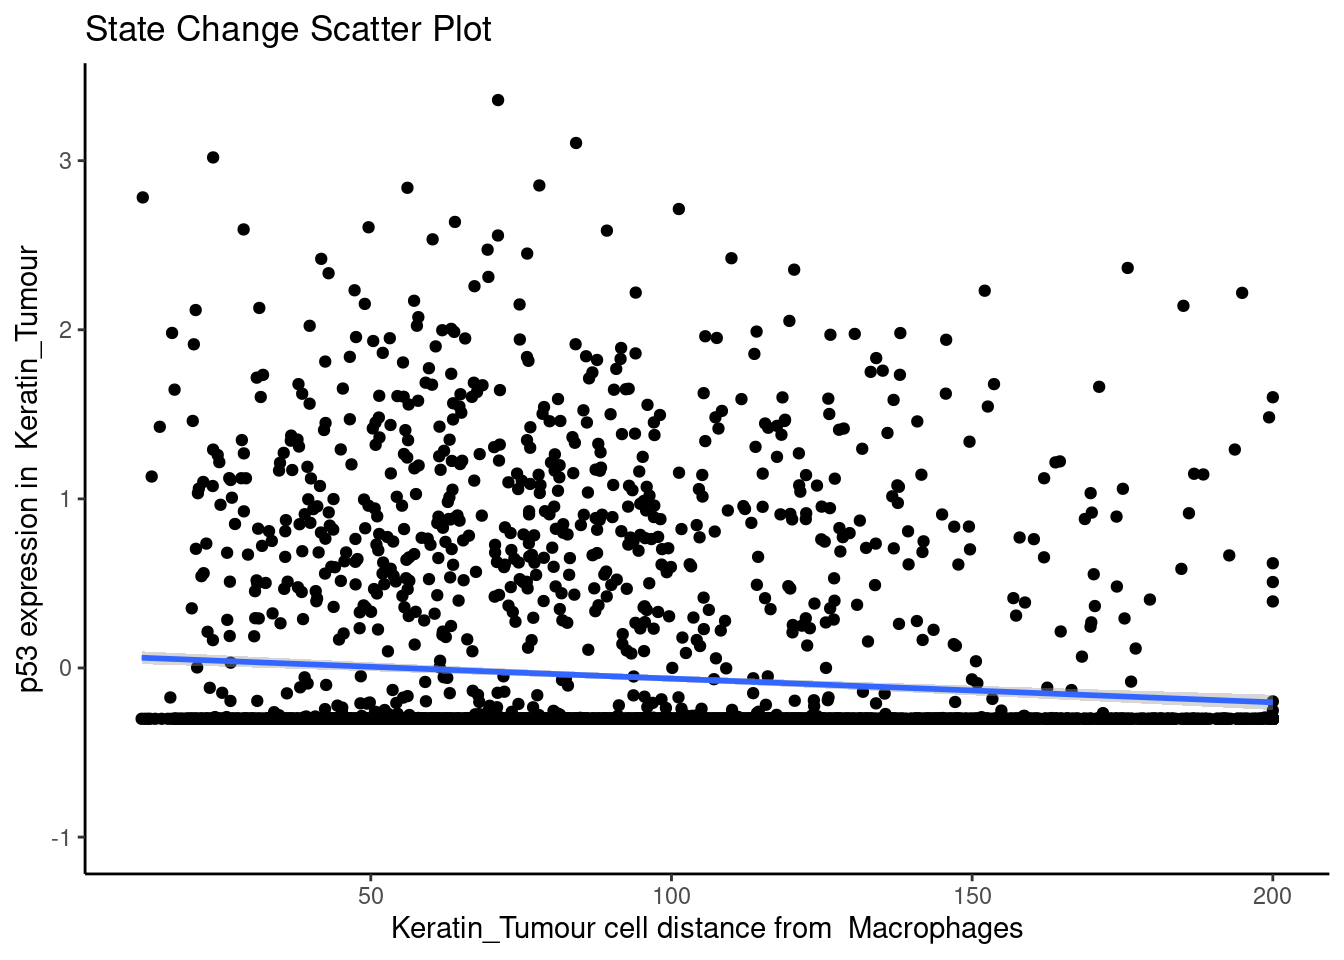
\includegraphics[keepaspectratio]{06-changes_in_marker_expression_files/figure-pdf/unnamed-chunk-6-2.pdf}}

\subsection{Continuous cell state changes across all
images}\label{continuous-cell-state-changes-across-all-images}

Beyond looking at single cell-to-cell interactions for a single image,
we can also look at all interactions across all images. The
\texttt{calcStateChanges} function provided by Statial can be expanded
for this exact purpose - by not specifying cell types, a marker, or an
image, \texttt{calcStateChanges} will examine the most significant
correlations between distance and marker expression across the entire
dataset. Here, we've filtered out the most significant interactions to
only include those found within image 6 of the Keren et al.~dataset.

\begin{Shaded}
\begin{Highlighting}[]
\NormalTok{stateChanges }\OtherTok{\textless{}{-}} \FunctionTok{calcStateChanges}\NormalTok{(}
  \AttributeTok{cells =}\NormalTok{ kerenSPE,}
  \AttributeTok{type =} \StringTok{"distances"}\NormalTok{,}
  \AttributeTok{nCores =} \DecValTok{1}\NormalTok{,}
  \AttributeTok{minCells =} \DecValTok{100}
\NormalTok{)}

\NormalTok{stateChanges }\SpecialCharTok{|\textgreater{}}
  \FunctionTok{filter}\NormalTok{(imageID }\SpecialCharTok{==} \DecValTok{6}\NormalTok{) }\SpecialCharTok{|\textgreater{}}
  \FunctionTok{head}\NormalTok{(}\AttributeTok{n =} \DecValTok{10}\NormalTok{)}
\end{Highlighting}
\end{Shaded}

\begin{verbatim}
   imageID primaryCellType otherCellType       marker         coef      tval
1        6  Keratin_Tumour  Unidentified           Na  0.004218419  25.03039
2        6  Keratin_Tumour   Macrophages  HLA_Class_1 -0.003823497 -24.69629
3        6  Keratin_Tumour    CD4_T_cell  HLA_Class_1 -0.003582774 -23.87797
4        6  Keratin_Tumour  Unidentified Beta.catenin  0.005893120  23.41953
5        6  Keratin_Tumour    CD8_T_cell  HLA_Class_1 -0.003154544 -23.13804
6        6  Keratin_Tumour    DC_or_Mono  HLA_Class_1 -0.003353834 -22.98944
7        6  Keratin_Tumour      dn_T_CD3  HLA_Class_1 -0.003123446 -22.63197
8        6  Keratin_Tumour        Tumour  HLA_Class_1  0.003684079  21.94265
9        6  Keratin_Tumour    CD4_T_cell           Fe -0.003457338 -21.43550
10       6  Keratin_Tumour    CD4_T_cell   phospho.S6 -0.002892457 -20.50767
            pval           fdr
1  6.971648e-127 3.382534e-123
2  7.814253e-124 3.430271e-120
3  1.745242e-116 5.362839e-113
4  1.917245e-112 5.523165e-109
5  5.444541e-110 1.434014e-106
6  1.053130e-108 2.696743e-105
7  1.237988e-105 2.889213e-102
8  8.188258e-100  1.640945e-96
9   1.287478e-95  2.260688e-92
10  3.928912e-88  5.748996e-85
\end{verbatim}

In image 6, the majority of the top 10 most significant interactions
occur between keratin/tumour cells and an immune population, and many of
these interactions appear to involve the HLA class I ligand.

We can examine some of these interactions further with the
\texttt{plotStateChanges} function. Taking a closer examination of the
relationship between macrophages and keratin/tumour HLA class I
expression, the plot below shows us a clear visual correlation - as
macrophage density increases, keratin/tumour cells increase their
expression HLA class I.

Biologically, HLA Class I is a ligand which exists on all nucleated
cells, tasked with presenting internal cell antigens for recognition by
the immune system, marking aberrant cells for destruction by either CD8+
T cells or NK cells.

\begin{Shaded}
\begin{Highlighting}[]
\NormalTok{p }\OtherTok{\textless{}{-}} \FunctionTok{plotStateChanges}\NormalTok{(}
  \AttributeTok{cells =}\NormalTok{ kerenSPE,}
  \AttributeTok{type =} \StringTok{"distances"}\NormalTok{,}
  \AttributeTok{image =} \StringTok{"6"}\NormalTok{,}
  \AttributeTok{from =} \StringTok{"Keratin\_Tumour"}\NormalTok{,}
  \AttributeTok{to =} \StringTok{"Macrophages"}\NormalTok{,}
  \AttributeTok{marker =} \StringTok{"HLA\_Class\_1"}\NormalTok{,}
  \AttributeTok{size =} \DecValTok{1}\NormalTok{,}
  \AttributeTok{shape =} \DecValTok{19}\NormalTok{,}
  \AttributeTok{interactive =} \ConstantTok{FALSE}\NormalTok{,}
  \AttributeTok{plotModelFit =} \ConstantTok{FALSE}\NormalTok{,}
  \AttributeTok{method =} \StringTok{"lm"}
\NormalTok{)}

\NormalTok{p}
\end{Highlighting}
\end{Shaded}

\begin{verbatim}
$image
\end{verbatim}

\pandocbounded{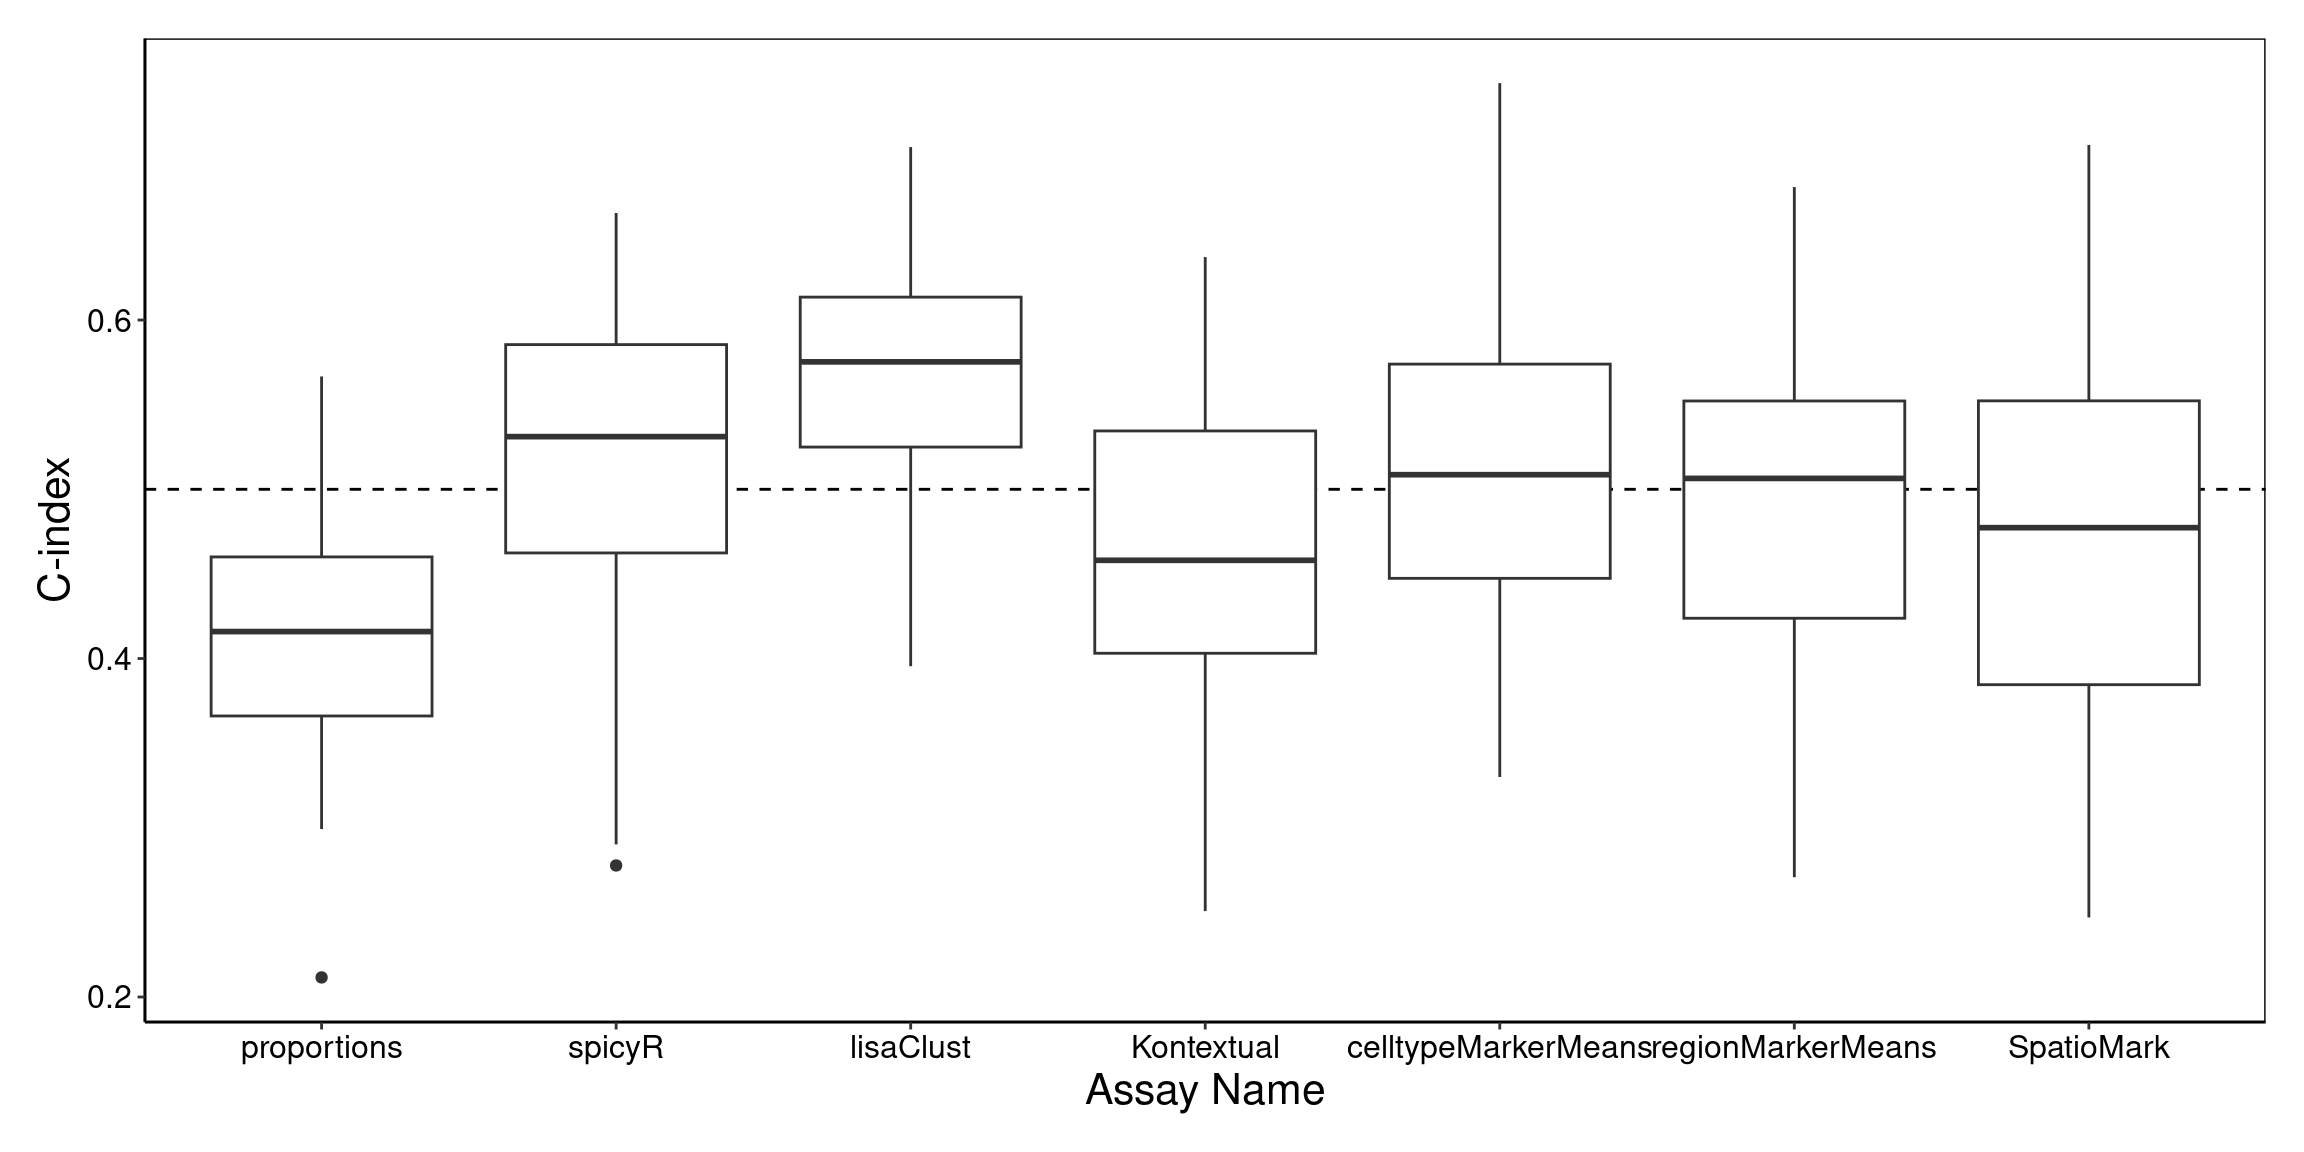
\includegraphics[keepaspectratio]{06-changes_in_marker_expression_files/figure-pdf/unnamed-chunk-8-1.pdf}}

\begin{verbatim}

$scatter
\end{verbatim}

\begin{verbatim}
`geom_smooth()` using formula = 'y ~ x'
\end{verbatim}

\begin{verbatim}
Warning: Removed 1359 rows containing non-finite outside the scale range
(`stat_smooth()`).
\end{verbatim}

\begin{verbatim}
Warning: Removed 1359 rows containing missing values or values outside the scale range
(`geom_point()`).
\end{verbatim}

\pandocbounded{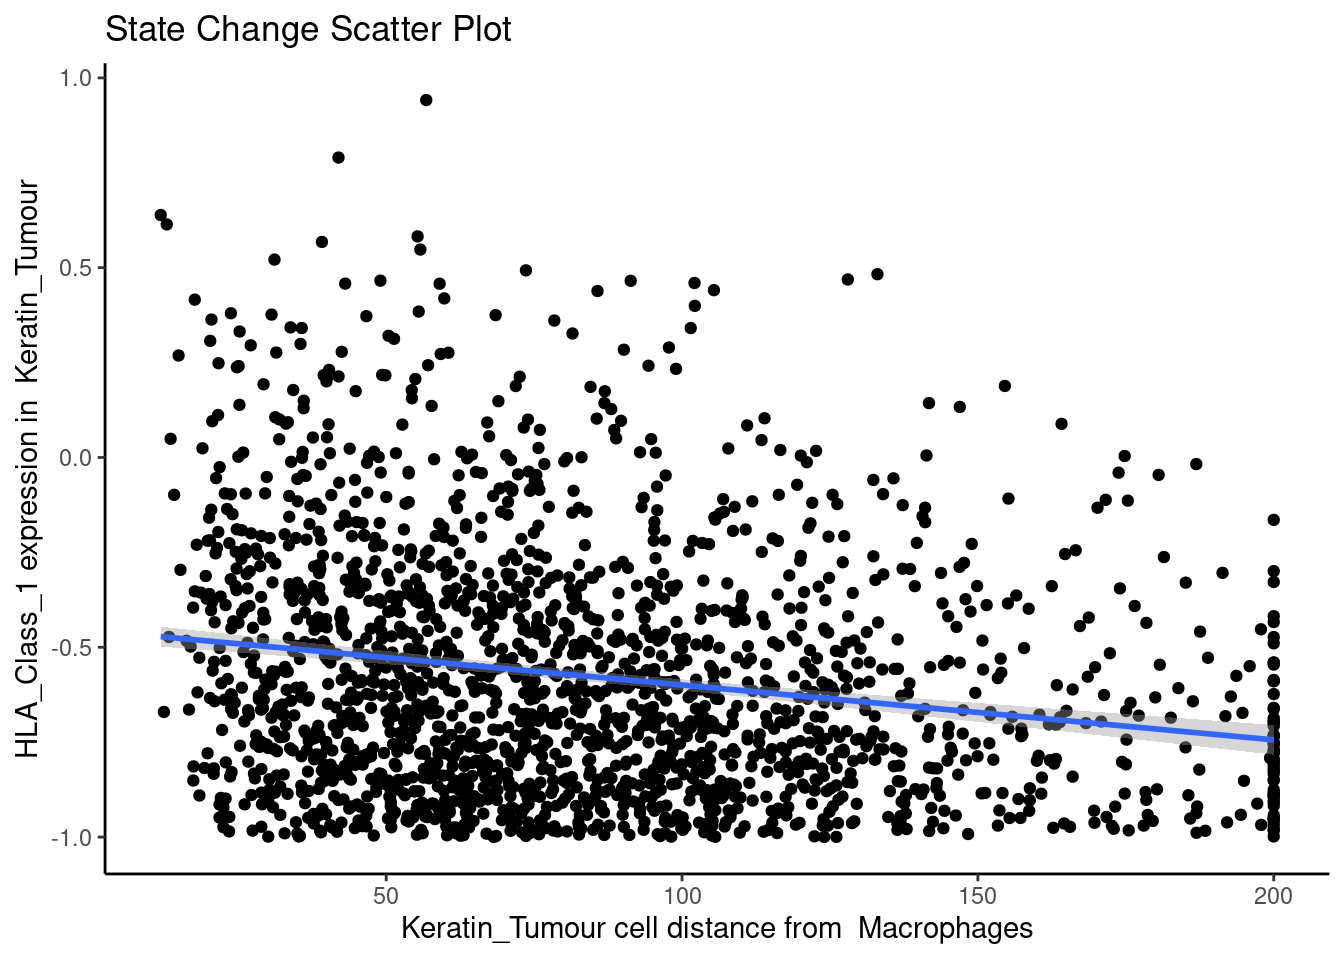
\includegraphics[keepaspectratio]{06-changes_in_marker_expression_files/figure-pdf/unnamed-chunk-8-2.pdf}}

Next, let's take a look at the top 10 most significant results across
all images.

\begin{Shaded}
\begin{Highlighting}[]
\NormalTok{stateChanges }\SpecialCharTok{|\textgreater{}} \FunctionTok{head}\NormalTok{(}\AttributeTok{n =} \DecValTok{10}\NormalTok{)}
\end{Highlighting}
\end{Shaded}

\begin{verbatim}
       imageID primaryCellType otherCellType     marker         coef
69468       37     Endothelial        Tumour       Lag3 -0.001621517
153135      11     Neutrophils            NK       CD56 -0.059936866
16402       35      CD4_T_cell        B_cell       CD20 -0.029185750
16498       35      CD4_T_cell    DC_or_Mono       CD20  0.019125946
4891        35          B_cell    DC_or_Mono phospho.S6  0.005282065
16507       35      CD4_T_cell    DC_or_Mono phospho.S6  0.004033218
4885        35          B_cell    DC_or_Mono     HLA.DR  0.011120703
5043        35          B_cell  Other_Immune          P  0.011182182
16354       35      CD4_T_cell      dn_T_CD3       CD20  0.016349492
4888        35          B_cell    DC_or_Mono     H3K9ac  0.005096632
                tval          pval           fdr
69468  -4.916884e+14  0.000000e+00  0.000000e+00
153135 -2.172437e+15  0.000000e+00  0.000000e+00
16402  -4.057355e+01 7.019343e-282 4.313854e-277
16498   4.053436e+01 1.891267e-281 8.717324e-277
4891    4.041385e+01 5.306590e-278 1.956752e-273
16507   3.472882e+01 4.519947e-219 1.388904e-214
4885    3.415344e+01 8.401034e-212 2.212712e-207
5043    3.414375e+01 1.056403e-211 2.434613e-207
16354   3.391901e+01 1.219488e-210 2.498188e-206
4888    3.399856e+01 3.266533e-210 6.022506e-206
\end{verbatim}

Immediately, we can appreciate that a couple of these interactions are
not biologically plausible. One of the most significant interactions
occurs between B cells and CD4 T cells in image 35, where CD4 T cells
are found to increase in CD20 expression when in close proximity to B
cells. Biologically, CD20 is a highly specific ligand for B cells, and
under healthy circumstances are usually not expressed in T cells.

Could this potentially be an artefact of \texttt{calcStateChanges}? We
can examine the image through the \texttt{plotStateChanges} function,
where we indeed observe a strong increase in CD20 expression in T cells
nearby B cell populations.

\begin{Shaded}
\begin{Highlighting}[]
\NormalTok{p }\OtherTok{\textless{}{-}} \FunctionTok{plotStateChanges}\NormalTok{(}
  \AttributeTok{cells =}\NormalTok{ kerenSPE,}
  \AttributeTok{type =} \StringTok{"distances"}\NormalTok{,}
  \AttributeTok{image =} \StringTok{"35"}\NormalTok{,}
  \AttributeTok{from =} \StringTok{"CD4\_T\_cell"}\NormalTok{,}
  \AttributeTok{to =} \StringTok{"B\_cell"}\NormalTok{,}
  \AttributeTok{marker =} \StringTok{"CD20"}\NormalTok{,}
  \AttributeTok{size =} \DecValTok{1}\NormalTok{,}
  \AttributeTok{shape =} \DecValTok{19}\NormalTok{,}
  \AttributeTok{interactive =} \ConstantTok{FALSE}\NormalTok{,}
  \AttributeTok{plotModelFit =} \ConstantTok{FALSE}\NormalTok{,}
  \AttributeTok{method =} \StringTok{"lm"}
\NormalTok{)}

\NormalTok{p}
\end{Highlighting}
\end{Shaded}

\begin{verbatim}
$image
\end{verbatim}

\pandocbounded{\includegraphics[keepaspectratio]{06-changes_in_marker_expression_files/figure-pdf/unnamed-chunk-10-1.pdf}}

\begin{verbatim}

$scatter
\end{verbatim}

\begin{verbatim}
`geom_smooth()` using formula = 'y ~ x'
\end{verbatim}

\begin{verbatim}
Warning: Removed 26 rows containing missing values or values outside the scale range
(`geom_smooth()`).
\end{verbatim}

\pandocbounded{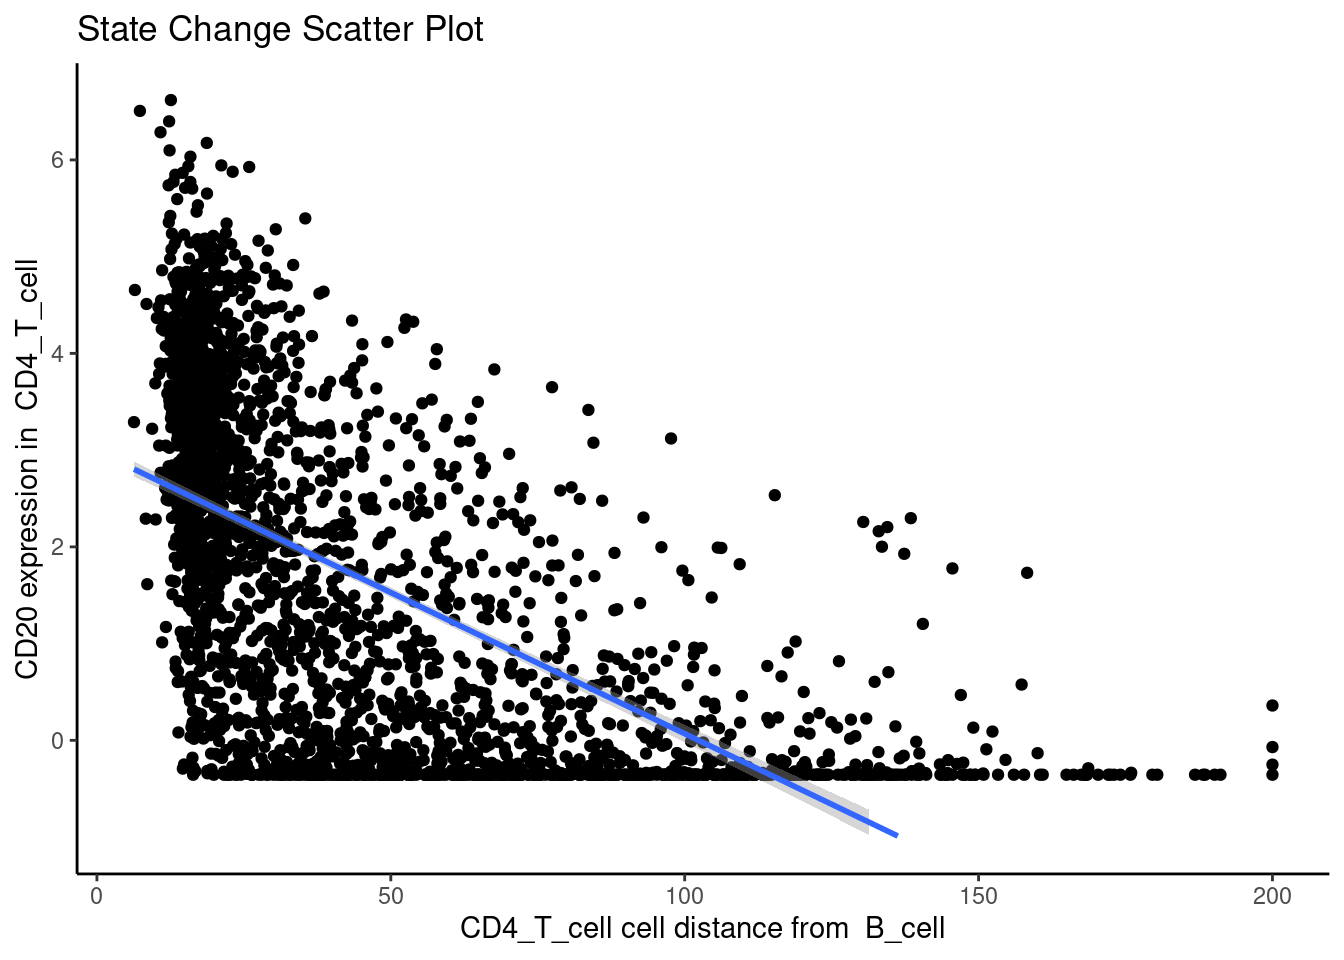
\includegraphics[keepaspectratio]{06-changes_in_marker_expression_files/figure-pdf/unnamed-chunk-10-2.pdf}}

So why are T cells expressing CD20? This brings us to a key problem of
cell segmentation - contamination.

\subsection{Contamination (Lateral marker spill
over)}\label{contamination-lateral-marker-spill-over}

Contamination, or lateral marker spill over is an issue that results in
a cell's marker expressions being wrongly attributed to another adjacent
cell. This issue arises from incorrect segmentation where components of
one cell are wrongly determined as belonging to another cell.
Alternatively, this issue can arise when antibodies used to tag and
measure marker expressions don't latch on properly to a cell of
interest, thereby resulting in residual markers being wrongly assigned
as belonging to a cell near the intended target cell. It is important
that we either correct or account for this incorrect attribution of
markers in our modelling process. This is critical in understanding
whether significant cell-cell interactions detected are an artefact of
technical measurement errors driven by spill over or are real biological
changes that represent a shift in a cell's state.

To circumvent this problem, Statial provides a function that predicts
the probability that a cell is any particular cell type -
\texttt{calcContamination}. \texttt{calcContamination} returns a
dataframe of probabilities demarcating the chance of a cell being any
particular cell type. This dataframe is stored under
\texttt{contaminations} in the \texttt{reducedDim} slot of the
\texttt{SingleCellExperiment} object. It also provides the
\texttt{rfMainCellProb} column, which provides the probability that a
cell is indeed the cell type it has been designated. E.g. For a cell
designated as CD8, rfMainCellProb could give a 80\% chance that the cell
is indeed CD8, due to contamination.

We can then introduce these probabilities as covariates into our linear
model by setting \texttt{contamination\ =\ TRUE} as a parameter in our
\texttt{calcStateChanges} function. However, this is not a perfect
solution for the issue of contamination. As we can see, despite
factoring in contamination into our linear model, the correlation
between B cell density and CD20 expression in CD4 T cells remains one of
the most significant interactions in our model.

\begin{Shaded}
\begin{Highlighting}[]
\NormalTok{kerenSPE }\OtherTok{\textless{}{-}} \FunctionTok{calcContamination}\NormalTok{(kerenSPE)}
\end{Highlighting}
\end{Shaded}

\begin{verbatim}
Growing trees.. Progress: 30%. Estimated remaining time: 1 minute, 12 seconds.
Growing trees.. Progress: 62%. Estimated remaining time: 39 seconds.
Growing trees.. Progress: 93%. Estimated remaining time: 7 seconds.
\end{verbatim}

\begin{Shaded}
\begin{Highlighting}[]
\NormalTok{stateChangesCorrected }\OtherTok{\textless{}{-}} \FunctionTok{calcStateChanges}\NormalTok{(}
  \AttributeTok{cells =}\NormalTok{ kerenSPE,}
  \AttributeTok{type =} \StringTok{"distances"}\NormalTok{,}
  \AttributeTok{nCores =} \DecValTok{1}\NormalTok{,}
  \AttributeTok{minCells =} \DecValTok{100}\NormalTok{,}
  \AttributeTok{contamination =} \ConstantTok{TRUE}
\NormalTok{)}

\NormalTok{stateChangesCorrected }\SpecialCharTok{|\textgreater{}} \FunctionTok{head}\NormalTok{(}\AttributeTok{n =} \DecValTok{20}\NormalTok{)}
\end{Highlighting}
\end{Shaded}

\begin{verbatim}
       imageID primaryCellType otherCellType      marker         coef
69468       37     Endothelial        Tumour        Lag3 -0.001621517
153135      11     Neutrophils            NK        CD56 -0.059936866
16402       35      CD4_T_cell        B_cell        CD20 -0.025155997
16498       35      CD4_T_cell    DC_or_Mono        CD20  0.016317938
16507       35      CD4_T_cell    DC_or_Mono  phospho.S6  0.003619727
16354       35      CD4_T_cell      dn_T_CD3        CD20  0.013869372
4891        35          B_cell    DC_or_Mono  phospho.S6  0.004279319
16357       35      CD4_T_cell      dn_T_CD3      HLA.DR  0.010366047
89188        3  Keratin_Tumour            DC          Ca -0.013725032
3697        28          B_cell            NK          Na -0.004437050
82222       20  Keratin_Tumour        Tumour HLA_Class_1  0.002922784
4741        35          B_cell      dn_T_CD3      HLA.DR  0.008880493
83998       23  Keratin_Tumour  Unidentified HLA_Class_1  0.003104015
16491       35      CD4_T_cell    DC_or_Mono      CSF.1R  0.008618601
82985       21  Keratin_Tumour            DC Pan.Keratin -0.005990784
16363       35      CD4_T_cell      dn_T_CD3  phospho.S6  0.002970004
99073        6  Keratin_Tumour  Unidentified          Na  0.004210683
4885        35          B_cell    DC_or_Mono      HLA.DR  0.008659992
82177       20  Keratin_Tumour        Tumour          Na  0.002528292
5083        35          B_cell  Other_Immune  phospho.S6  0.004549575
                tval          pval           fdr
69468  -3.668163e+14  0.000000e+00  0.000000e+00
153135 -1.469129e+17  0.000000e+00  0.000000e+00
16402  -3.503922e+01 4.151258e-222 2.551225e-217
16498   3.451351e+01 1.286531e-216 5.929942e-212
16507   2.995929e+01 1.502564e-170 5.540553e-166
16354   2.994028e+01 2.305225e-170 7.083573e-166
4891    2.953140e+01 1.404125e-165 3.698265e-161
16357   2.920130e+01 3.488396e-163 8.039445e-159
89188  -2.940905e+01 6.078033e-161 1.245119e-156
3697   -2.890578e+01 2.110059e-156 3.890316e-152
82222   2.563648e+01 1.248985e-132 2.093412e-128
4741    2.580213e+01 6.315062e-131 9.702567e-127
83998   2.513875e+01 2.869643e-128 4.069816e-124
16491   2.539208e+01 9.301666e-128 1.224963e-123
82985  -2.470505e+01 8.193691e-127 1.007114e-122
16363   2.510997e+01 2.992332e-125 3.448101e-121
99073   2.468985e+01 9.949871e-124 1.079093e-119
4885    2.465260e+01 8.651171e-121 8.861202e-117
82177   2.424891e+01 6.517655e-120 6.324526e-116
5083    2.425395e+01 2.432632e-117 2.242522e-113
\end{verbatim}

However, this does not mean factoring in contamination into our linear
model was ineffective.

Whilst our correction attempts do not rectify every relationship which
arises due to contamination, we show that a significant portion of these
relationships are rectified. We can show this by plotting a ROC curve of
true positives against false positives. In general, cell type specific
markers such as CD4, CD8, and CD20 should not change in cells they are
not specific to. Therefore, relationships detected to be significant
involving these cell type markers are likely false positives and will be
treated as such for the purposes of evaluation. Meanwhile, cell state
markers are predominantly likely to be true positives.

Plotting the relationship between false positives and true positives,
we'd expect the contamination correction to be greatest in the
relationships with the top 100 lowest p values, where we indeed see more
true positives than false positives with contamination correction.

\begin{Shaded}
\begin{Highlighting}[]
\NormalTok{cellTypeMarkers }\OtherTok{\textless{}{-}} \FunctionTok{c}\NormalTok{(}\StringTok{"CD3"}\NormalTok{, }\StringTok{"CD4"}\NormalTok{, }\StringTok{"CD8"}\NormalTok{, }\StringTok{"CD56"}\NormalTok{, }\StringTok{"CD11c"}\NormalTok{, }\StringTok{"CD68"}\NormalTok{, }\StringTok{"CD45"}\NormalTok{, }\StringTok{"CD20"}\NormalTok{)}

\NormalTok{values }\OtherTok{\textless{}{-}} \FunctionTok{c}\NormalTok{(}\StringTok{"blue"}\NormalTok{, }\StringTok{"red"}\NormalTok{)}
\FunctionTok{names}\NormalTok{(values) }\OtherTok{\textless{}{-}} \FunctionTok{c}\NormalTok{(}\StringTok{"None"}\NormalTok{, }\StringTok{"Corrected"}\NormalTok{)}

\NormalTok{df }\OtherTok{\textless{}{-}} \FunctionTok{rbind}\NormalTok{(}
  \FunctionTok{data.frame}\NormalTok{(}\AttributeTok{TP =} \FunctionTok{cumsum}\NormalTok{(stateChanges}\SpecialCharTok{$}\NormalTok{marker }\SpecialCharTok{\%in\%}\NormalTok{ cellTypeMarkers), }\AttributeTok{FP =} \FunctionTok{cumsum}\NormalTok{(}\SpecialCharTok{!}\NormalTok{stateChanges}\SpecialCharTok{$}\NormalTok{marker }\SpecialCharTok{\%in\%}\NormalTok{ cellTypeMarkers), }\AttributeTok{type =} \StringTok{"None"}\NormalTok{),}
  \FunctionTok{data.frame}\NormalTok{(}\AttributeTok{TP =} \FunctionTok{cumsum}\NormalTok{(stateChangesCorrected}\SpecialCharTok{$}\NormalTok{marker }\SpecialCharTok{\%in\%}\NormalTok{ cellTypeMarkers), }\AttributeTok{FP =} \FunctionTok{cumsum}\NormalTok{(}\SpecialCharTok{!}\NormalTok{stateChangesCorrected}\SpecialCharTok{$}\NormalTok{marker }\SpecialCharTok{\%in\%}\NormalTok{ cellTypeMarkers), }\AttributeTok{type =} \StringTok{"Corrected"}\NormalTok{)}
\NormalTok{)}

\FunctionTok{ggplot}\NormalTok{(df, }\FunctionTok{aes}\NormalTok{(}\AttributeTok{x =}\NormalTok{ TP, }\AttributeTok{y =}\NormalTok{ FP, }\AttributeTok{colour =}\NormalTok{ type)) }\SpecialCharTok{+}
  \FunctionTok{geom\_line}\NormalTok{() }\SpecialCharTok{+}
  \FunctionTok{labs}\NormalTok{(}\AttributeTok{y =} \StringTok{"Cell state marker"}\NormalTok{, }\AttributeTok{x =} \StringTok{"Cell type marker"}\NormalTok{) }\SpecialCharTok{+}
  \FunctionTok{scale\_colour\_manual}\NormalTok{(}\AttributeTok{values =}\NormalTok{ values)}
\end{Highlighting}
\end{Shaded}

\pandocbounded{\includegraphics[keepaspectratio]{06-changes_in_marker_expression_files/figure-pdf/unnamed-chunk-12-1.pdf}}

Here, we zoom in on the ROC curve where the top 100 lowest p values
occur, where we indeed see more true positives than false positives with
contamination correction.

\begin{Shaded}
\begin{Highlighting}[]
\FunctionTok{ggplot}\NormalTok{(df, }\FunctionTok{aes}\NormalTok{(}\AttributeTok{x =}\NormalTok{ TP, }\AttributeTok{y =}\NormalTok{ FP, }\AttributeTok{colour =}\NormalTok{ type)) }\SpecialCharTok{+}
  \FunctionTok{geom\_line}\NormalTok{() }\SpecialCharTok{+}
  \FunctionTok{xlim}\NormalTok{(}\DecValTok{0}\NormalTok{, }\DecValTok{100}\NormalTok{) }\SpecialCharTok{+}
  \FunctionTok{ylim}\NormalTok{(}\DecValTok{0}\NormalTok{, }\DecValTok{1000}\NormalTok{) }\SpecialCharTok{+}
  \FunctionTok{labs}\NormalTok{(}\AttributeTok{y =} \StringTok{"Cell state marker"}\NormalTok{, }\AttributeTok{x =} \StringTok{"Cell type marker"}\NormalTok{) }\SpecialCharTok{+}
  \FunctionTok{scale\_colour\_manual}\NormalTok{(}\AttributeTok{values =}\NormalTok{ values)}
\end{Highlighting}
\end{Shaded}

\begin{verbatim}
Warning: Removed 371471 rows containing missing values or values outside the scale range
(`geom_line()`).
\end{verbatim}

\pandocbounded{\includegraphics[keepaspectratio]{06-changes_in_marker_expression_files/figure-pdf/unnamed-chunk-13-1.pdf}}

\subsection{Associate continuous state changes with survival
outcomes}\label{associate-continuous-state-changes-with-survival-outcomes}

Similiar to \texttt{Kontextual}, we can run a similar survival analysis
using our state changes results. Here, \texttt{prepMatrix} extracts the
coefficients, or the \texttt{coef} column of \texttt{stateChanges} by
default. To use the t values instead, specify \texttt{column\ =\ "tval"}
in the \texttt{prepMatrix} function.

\begin{Shaded}
\begin{Highlighting}[]
\CommentTok{\# Preparing features for Statial}
\NormalTok{stateMat }\OtherTok{\textless{}{-}} \FunctionTok{prepMatrix}\NormalTok{(stateChanges)}

\CommentTok{\# Ensuring rownames of stateMat match up with rownames of the survival vector}
\NormalTok{stateMat }\OtherTok{\textless{}{-}}\NormalTok{ stateMat[}\FunctionTok{names}\NormalTok{(kerenSurv), ]}

\CommentTok{\# Remove some very small values}
\NormalTok{stateMat }\OtherTok{\textless{}{-}}\NormalTok{ stateMat[, }\FunctionTok{colMeans}\NormalTok{(}\FunctionTok{abs}\NormalTok{(stateMat) }\SpecialCharTok{\textgreater{}} \FloatTok{0.0001}\NormalTok{) }\SpecialCharTok{\textgreater{}}\NormalTok{ .}\DecValTok{8}\NormalTok{]}

\NormalTok{survivalResults }\OtherTok{\textless{}{-}} \FunctionTok{colTest}\NormalTok{(stateMat, kerenSurv, }\AttributeTok{type =} \StringTok{"survival"}\NormalTok{)}

\FunctionTok{head}\NormalTok{(survivalResults)}
\end{Highlighting}
\end{Shaded}

\begin{verbatim}
                                         coef se.coef   pval adjPval
Keratin_Tumour__Mono_or_Neu__Pan.Keratin -280      89 0.0018    0.63
Macrophages__Keratin_Tumour__HLA_Class_1  220      75 0.0034    0.63
Keratin_Tumour__CD8_T_cell__Keratin6     -220      77 0.0036    0.63
Macrophages__Other_Immune__HLA_Class_1   -480     170 0.0057    0.75
Keratin_Tumour__Mesenchymal__dsDNA       -810     310 0.0094    0.80
Keratin_Tumour__Unidentified__H3K27me3    490     190 0.0100    0.80
                                                                          cluster
Keratin_Tumour__Mono_or_Neu__Pan.Keratin Keratin_Tumour__Mono_or_Neu__Pan.Keratin
Macrophages__Keratin_Tumour__HLA_Class_1 Macrophages__Keratin_Tumour__HLA_Class_1
Keratin_Tumour__CD8_T_cell__Keratin6         Keratin_Tumour__CD8_T_cell__Keratin6
Macrophages__Other_Immune__HLA_Class_1     Macrophages__Other_Immune__HLA_Class_1
Keratin_Tumour__Mesenchymal__dsDNA             Keratin_Tumour__Mesenchymal__dsDNA
Keratin_Tumour__Unidentified__H3K27me3     Keratin_Tumour__Unidentified__H3K27me3
\end{verbatim}

For our state changes results,
\texttt{Keratin\_Tumour\_\_CD4\_Cell\_\_Keratin6} is the most
significant pairwise relationship which contributes to patient survival.
That is, the relationship between HLA class I expression in
keratin/tumour cells and their spatial proximity to mesenchymal cells.
As there is a negative coeffcient associated with this relationship,
which tells us that higher HLA class I expression in keratin/tumour
cells nearby mesenchymal cell populations lead to poorer survival
outcomes for patients.

\begin{Shaded}
\begin{Highlighting}[]
\CommentTok{\# Selecting the most significant relationship}
\NormalTok{survRelationship }\OtherTok{\textless{}{-}}\NormalTok{ stateMat[[}\StringTok{"Keratin\_Tumour\_\_Mono\_or\_Neu\_\_Pan.Keratin"}\NormalTok{]]}
\NormalTok{survRelationship }\OtherTok{\textless{}{-}} \FunctionTok{ifelse}\NormalTok{(survRelationship }\SpecialCharTok{\textgreater{}} \FunctionTok{median}\NormalTok{(survRelationship), }\StringTok{"Higher expression in close cells"}\NormalTok{, }\StringTok{"Lower expression in close cells"}\NormalTok{)}

\CommentTok{\# Plotting Kaplan{-}Meier curve}
\FunctionTok{survfit2}\NormalTok{(kerenSurv }\SpecialCharTok{\textasciitilde{}}\NormalTok{ survRelationship) }\SpecialCharTok{|\textgreater{}}
  \FunctionTok{ggsurvfit}\NormalTok{() }\SpecialCharTok{+}
  \FunctionTok{add\_pvalue}\NormalTok{() }\SpecialCharTok{+}
  \FunctionTok{ggtitle}\NormalTok{(}\StringTok{"Keratin\_Tumour\_\_Mono\_or\_Neu\_\_Pan.Keratin"}\NormalTok{)}
\end{Highlighting}
\end{Shaded}

\pandocbounded{\includegraphics[keepaspectratio]{06-changes_in_marker_expression_files/figure-pdf/unnamed-chunk-15-1.pdf}}

\section{scFeatures: Moran's I}\label{scfeatures-morans-i}

\section{sessionInfo}\label{sessioninfo-5}

\begin{Shaded}
\begin{Highlighting}[]
\FunctionTok{sessionInfo}\NormalTok{()}
\end{Highlighting}
\end{Shaded}

\begin{verbatim}
R version 4.4.1 (2024-06-14)
Platform: x86_64-pc-linux-gnu
Running under: Debian GNU/Linux 12 (bookworm)

Matrix products: default
BLAS:   /usr/lib/x86_64-linux-gnu/openblas-pthread/libblas.so.3 
LAPACK: /usr/lib/x86_64-linux-gnu/openblas-pthread/libopenblasp-r0.3.21.so;  LAPACK version 3.11.0

locale:
 [1] LC_CTYPE=C.UTF-8       LC_NUMERIC=C           LC_TIME=C.UTF-8       
 [4] LC_COLLATE=C.UTF-8     LC_MONETARY=C.UTF-8    LC_MESSAGES=C.UTF-8   
 [7] LC_PAPER=C.UTF-8       LC_NAME=C              LC_ADDRESS=C          
[10] LC_TELEPHONE=C         LC_MEASUREMENT=C.UTF-8 LC_IDENTIFICATION=C   

time zone: Australia/Sydney
tzcode source: system (glibc)

attached base packages:
[1] stats4    stats     graphics  grDevices utils     datasets  methods  
[8] base     

other attached packages:
 [1] SpatialDatasets_1.4.0       SpatialExperiment_1.16.0   
 [3] ExperimentHub_2.14.0        AnnotationHub_3.14.0       
 [5] BiocFileCache_2.14.0        dbplyr_2.5.0               
 [7] Statial_1.7.4               testthat_3.2.1.1           
 [9] treekoR_1.14.0              tibble_3.2.1               
[11] ggsurvfit_1.1.0             ggplot2_3.5.1              
[13] SingleCellExperiment_1.28.1 dplyr_1.1.4                
[15] lisaClust_1.14.4            ClassifyR_3.10.0           
[17] survival_3.7-0              BiocParallel_1.40.0        
[19] MultiAssayExperiment_1.32.0 SummarizedExperiment_1.36.0
[21] Biobase_2.66.0              GenomicRanges_1.58.0       
[23] GenomeInfoDb_1.42.0         IRanges_2.40.0             
[25] MatrixGenerics_1.18.0       matrixStats_1.4.1          
[27] S4Vectors_0.44.0            BiocGenerics_0.52.0        
[29] generics_0.1.3              spicyR_1.18.0              

loaded via a namespace (and not attached):
  [1] fs_1.6.5                    spatstat.sparse_3.1-0      
  [3] devtools_2.4.5              httr_1.4.7                 
  [5] hopach_2.66.0               RColorBrewer_1.1-3         
  [7] doParallel_1.0.17           numDeriv_2016.8-1.1        
  [9] profvis_0.4.0               tools_4.4.1                
 [11] backports_1.5.0             utf8_1.2.4                 
 [13] R6_2.5.1                    lazyeval_0.2.2             
 [15] mgcv_1.9-1                  GetoptLong_1.0.5           
 [17] urlchecker_1.0.1            withr_3.0.2                
 [19] coxme_2.2-22                cli_3.6.3                  
 [21] spatstat.explore_3.3-3      sandwich_3.1-1             
 [23] labeling_0.4.3              mvtnorm_1.3-2              
 [25] spatstat.data_3.1-2         systemfonts_1.1.0          
 [27] yulab.utils_0.1.8           ggupset_0.4.0              
 [29] colorRamps_2.3.4            sessioninfo_1.2.2          
 [31] limma_3.62.1                RSQLite_2.3.7              
 [33] flowCore_2.18.0             rstudioapi_0.17.1          
 [35] gridGraphics_0.5-1          shape_1.4.6.1              
 [37] spatstat.random_3.3-2       car_3.1-3                  
 [39] scam_1.2-17                 Matrix_1.7-1               
 [41] RProtoBufLib_2.18.0         fansi_1.0.6                
 [43] abind_1.4-8                 lifecycle_1.0.4            
 [45] yaml_2.3.10                 multcomp_1.4-26            
 [47] edgeR_4.4.0                 carData_3.0-5              
 [49] SparseArray_1.6.0           Rtsne_0.17                 
 [51] blob_1.2.4                  grid_4.4.1                 
 [53] promises_1.3.0              crayon_1.5.3               
 [55] bdsmatrix_1.3-7             miniUI_0.1.1.1             
 [57] lattice_0.22-6              KEGGREST_1.46.0            
 [59] magick_2.8.5                pillar_1.9.0               
 [61] knitr_1.49                  ComplexHeatmap_2.22.0      
 [63] rjson_0.2.23                boot_1.3-31                
 [65] codetools_0.2-20            glue_1.8.0                 
 [67] ggiraph_0.8.10              ggfun_0.1.7                
 [69] spatstat.univar_3.1-1       data.table_1.16.2          
 [71] remotes_2.5.0               vctrs_0.6.5                
 [73] png_0.1-8                   treeio_1.30.0              
 [75] gtable_0.3.6                cachem_1.1.0               
 [77] xfun_0.49                   S4Arrays_1.6.0             
 [79] mime_0.12                   ConsensusClusterPlus_1.70.0
 [81] pheatmap_1.0.12             iterators_1.0.14           
 [83] tinytex_0.54                cytolib_2.18.0             
 [85] statmod_1.5.0               ellipsis_0.3.2             
 [87] TH.data_1.1-2               nlme_3.1-166               
 [89] usethis_3.0.0               ggtree_3.14.0              
 [91] bit64_4.5.2                 filelock_1.0.3             
 [93] rprojroot_2.0.4             DBI_1.2.3                  
 [95] colorspace_2.1-1            tidyselect_1.2.1           
 [97] curl_6.0.1                  bit_4.5.0                  
 [99] compiler_4.4.1              diffcyt_1.26.0             
[101] desc_1.4.3                  DelayedArray_0.32.0        
[103] plotly_4.10.4               scales_1.3.0               
[105] rappdirs_0.3.3              stringr_1.5.1              
[107] digest_0.6.37               goftest_1.2-3              
[109] fftwtools_0.9-11            spatstat.utils_3.1-1       
[111] minqa_1.2.8                 rmarkdown_2.29             
[113] XVector_0.46.0              htmltools_0.5.8.1          
[115] pkgconfig_2.0.3             lme4_1.1-35.5              
[117] fastmap_1.2.0               rlang_1.1.4                
[119] GlobalOptions_0.1.2         htmlwidgets_1.6.4          
[121] ggthemes_5.1.0              UCSC.utils_1.2.0           
[123] shiny_1.9.1                 ggh4x_0.2.8                
[125] farver_2.1.2                zoo_1.8-12                 
[127] jsonlite_1.8.9              magrittr_2.0.3             
[129] Formula_1.2-5               GenomeInfoDbData_1.2.13    
[131] ggplotify_0.1.2             patchwork_1.3.0            
[133] munsell_0.5.1               Rcpp_1.0.13-1              
[135] ape_5.8                     ggnewscale_0.5.0           
[137] stringi_1.8.4               brio_1.1.5                 
[139] zlibbioc_1.52.0             MASS_7.3-61                
[141] plyr_1.8.9                  pkgbuild_1.4.5             
[143] parallel_4.4.1              deldir_2.0-4               
[145] Biostrings_2.74.0           splines_4.4.1              
[147] tensor_1.5                  circlize_0.4.16            
[149] locfit_1.5-9.10             igraph_2.1.1               
[151] ggpubr_0.6.0                uuid_1.2-1                 
[153] ranger_0.17.0               spatstat.geom_3.3-3        
[155] ggsignif_0.6.4              reshape2_1.4.4             
[157] pkgload_1.4.0               BiocVersion_3.20.0         
[159] XML_3.99-0.17               evaluate_1.0.1             
[161] BiocManager_1.30.25         nloptr_2.1.1               
[163] foreach_1.5.2               tweenr_2.0.3               
[165] httpuv_1.6.15               tidyr_1.3.1                
[167] purrr_1.0.2                 polyclip_1.10-7            
[169] clue_0.3-66                 ggforce_0.4.2              
[171] broom_1.0.7                 xtable_1.8-4               
[173] tidytree_0.4.6              rstatix_0.7.2              
[175] later_1.3.2                 viridisLite_0.4.2          
[177] class_7.3-22                lmerTest_3.1-3             
[179] aplot_0.2.3                 AnnotationDbi_1.68.0       
[181] memoise_2.0.1               FlowSOM_2.14.0             
[183] cluster_2.1.6               concaveman_1.1.0           
\end{verbatim}

\bookmarksetup{startatroot}

\chapter{Classification}\label{classification}

Steps:

\begin{enumerate}
\def\labelenumi{\arabic{enumi}.}
\tightlist
\item
  Motivation of classification (prediction)
\item
  Classification of patients by condition
\item
  Classification of patients by survival
\item
  Easy and Hard to classify patients (samplesMetricMap)
\item
  Maximising accuracy during classification (parameter tuning for
  crossValidate)
\end{enumerate}

\section{Why classify?}\label{why-classify}

When it comes to biological datasets, the end goal is either mechanistic
or translational. For example, if we had a mechanistic end goal, we
might want to find what genes are differentially expressed between two
conditions, and further aim to characterise the pathways which lead to
this differential expression. Alternatively, if the end goal is
translational, we might want to use a biological dataset that can be
relatively cheaply obtained (e.g.~IMC) to predict whether a patient's
disease will progress or not progress (e.g.~metastasize in cancer).

Regardless of the end goal, classification is an important end-point for
any biological dataset, as it provides us information on:

\begin{enumerate}
\def\labelenumi{\arabic{enumi}.}
\tightlist
\item
  Important features
\item
  Predictability of the full dataset, or a subset of the dataset
\end{enumerate}

\texttt{ClassifyR} simplifies the process of classification, and
provides quick and simple ways to analyse datasets and determine how
well biological datasets can be classified into disease states using
particular feature generation techniques. In this chapter, we will
provide a guide on how to use \texttt{ClassifyR} on biological datasets,
and typical workflows for classification.

\section{Cross validation}\label{cross-validation}

Cross validation is an essential part of any classification process, and
is necessary to robustly determine how well your model has performed.
\texttt{ClassifyR} makes this extremely easy to implement with the
\texttt{crossValidate} function.

\begin{Shaded}
\begin{Highlighting}[]
\FunctionTok{library}\NormalTok{(ClassifyR)}
\FunctionTok{library}\NormalTok{(lisaClust)}

\NormalTok{BPPARAM }\OtherTok{\textless{}{-}}\NormalTok{ simpleSeg}\SpecialCharTok{:::}\FunctionTok{generateBPParam}\NormalTok{(}\AttributeTok{cores =} \DecValTok{40}\NormalTok{)}
\end{Highlighting}
\end{Shaded}

Using all the features we've generated in the previous chapters, we can
build a list of features matrices.

\begin{Shaded}
\begin{Highlighting}[]
\NormalTok{kerenSPE }\OtherTok{\textless{}{-}}\NormalTok{ SpatialDatasets}\SpecialCharTok{::}\FunctionTok{spe\_Keren\_2018}\NormalTok{()}
\end{Highlighting}
\end{Shaded}

\begin{verbatim}
see ?SpatialDatasets and browseVignettes('SpatialDatasets') for documentation
\end{verbatim}

\begin{verbatim}
loading from cache
\end{verbatim}

\bookmarksetup{startatroot}

\chapter{Case Study: Head and Neck Squamous Cell Carcinoma (Ferguson et
al.,
2022)}\label{case-study-head-and-neck-squamous-cell-carcinoma-ferguson-et-al.-2022}

\section{Load libraries}\label{load-libraries}

\begin{Shaded}
\begin{Highlighting}[]
\FunctionTok{library}\NormalTok{(cytomapper)}
\FunctionTok{library}\NormalTok{(dplyr)}
\FunctionTok{library}\NormalTok{(ggplot2)}
\FunctionTok{library}\NormalTok{(simpleSeg)}
\FunctionTok{library}\NormalTok{(FuseSOM)}
\FunctionTok{library}\NormalTok{(ggpubr)}
\FunctionTok{library}\NormalTok{(scater)}
\FunctionTok{library}\NormalTok{(spicyR)}
\FunctionTok{library}\NormalTok{(ClassifyR)}
\FunctionTok{library}\NormalTok{(lisaClust)}
\FunctionTok{library}\NormalTok{(Statial)}
\FunctionTok{library}\NormalTok{(tidySingleCellExperiment)}
\FunctionTok{library}\NormalTok{(SpatialExperiment)}
\FunctionTok{library}\NormalTok{(SpatialDatasets)}
\end{Highlighting}
\end{Shaded}

\section{Global parameters}\label{global-parameters}

It is convenient to set the number of cores for running code in
parallel. Please choose a number that is appropriate for your resources.
Set the \texttt{use\_mc} flag to \texttt{TRUE} if you would like to use
parallel processing for the rest of the vignette. A minimum of 2 cores
is suggested since running this workflow is rather computationally
intensive.

\begin{Shaded}
\begin{Highlighting}[]
\NormalTok{use\_mc }\OtherTok{\textless{}{-}} \ConstantTok{TRUE}

\ControlFlowTok{if}\NormalTok{ (use\_mc) \{}
\NormalTok{  nCores }\OtherTok{\textless{}{-}} \FunctionTok{max}\NormalTok{(parallel}\SpecialCharTok{::}\FunctionTok{detectCores}\NormalTok{()}\SpecialCharTok{/}\DecValTok{2}\NormalTok{, }\DecValTok{1}\NormalTok{)}
\NormalTok{\} }\ControlFlowTok{else}\NormalTok{ \{}
\NormalTok{  nCores }\OtherTok{\textless{}{-}} \DecValTok{2}
\NormalTok{\}}
\NormalTok{BPPARAM }\OtherTok{\textless{}{-}}\NormalTok{ simpleSeg}\SpecialCharTok{:::}\FunctionTok{generateBPParam}\NormalTok{(nCores)}

\FunctionTok{theme\_set}\NormalTok{(}\FunctionTok{theme\_classic}\NormalTok{())}
\end{Highlighting}
\end{Shaded}

\section{Context}\label{context}

In the following we will re-analyse some IMC data
\href{https://doi.org/10.1158/1078-0432.CCR-22-1332}{(Ferguson et al,
2022)} profiling the spatial landscape of head and neck cutaneous
squamous cell carcinomas (HNcSCC), the second most common type of skin
cancer. The majority of HNcSCC can be treated with surgery and good
local control, but a subset of large tumours infiltrate subcutaneous
tissue and are considered high risk for local recurrence and metastases.
The key conclusion of this manuscript (amongst others) is that spatial
information about cells and the immune environment can be used to
predict primary tumour progression or metastases in patients. We will
use our spicy workflow to reach a similar conclusion.

The R code for this analysis is available on github
\url{https://github.com/SydneyBioX/spicyWorkflow}.

\section{Read in images}\label{read-in-images}

Once the spicyWorkflow package is installed, these images will be
located within the \texttt{spicyWorkflow} folder where the
\texttt{spicyWorkflow} package is installed, under
\texttt{inst/extdata/images}. Here we use \texttt{loadImages()} from the
\texttt{cytomapper} package to load all the tiff images into a
\texttt{CytoImageList} object and store the images as h5 file on-disk in
a temporary directory using the
\texttt{h5FilesPath\ =\ HDF5Array::getHDF5DumpDir()} parameter.

We will also assign the metadata columns of the \texttt{CytoImageList}
object using the \texttt{mcols()} function.

\begin{Shaded}
\begin{Highlighting}[]
\NormalTok{pathToImages }\OtherTok{\textless{}{-}}\NormalTok{ SpatialDatasets}\SpecialCharTok{::}\FunctionTok{Ferguson\_Images}\NormalTok{()}
\end{Highlighting}
\end{Shaded}

\begin{verbatim}
see ?SpatialDatasets and browseVignettes('SpatialDatasets') for documentation
\end{verbatim}

\begin{verbatim}
loading from cache
\end{verbatim}

\begin{Shaded}
\begin{Highlighting}[]
\NormalTok{tmp }\OtherTok{\textless{}{-}} \FunctionTok{tempfile}\NormalTok{()}
\FunctionTok{unzip}\NormalTok{(pathToImages, }\AttributeTok{exdir =}\NormalTok{ tmp)}

\CommentTok{\# Store images in a CytoImageList on\_disk as h5 files to save memory.}
\NormalTok{images }\OtherTok{\textless{}{-}}\NormalTok{ cytomapper}\SpecialCharTok{::}\FunctionTok{loadImages}\NormalTok{(}
\NormalTok{  tmp,}
  \AttributeTok{single\_channel =} \ConstantTok{TRUE}\NormalTok{,}
  \AttributeTok{on\_disk =} \ConstantTok{TRUE}\NormalTok{,}
  \AttributeTok{h5FilesPath =}\NormalTok{ HDF5Array}\SpecialCharTok{::}\FunctionTok{getHDF5DumpDir}\NormalTok{(),}
  \AttributeTok{BPPARAM =}\NormalTok{ BPPARAM}
\NormalTok{)}

\FunctionTok{mcols}\NormalTok{(images) }\OtherTok{\textless{}{-}}\NormalTok{ S4Vectors}\SpecialCharTok{::}\FunctionTok{DataFrame}\NormalTok{(}\AttributeTok{imageID =} \FunctionTok{names}\NormalTok{(images))}
\end{Highlighting}
\end{Shaded}

\subsection{Clean channel names}\label{clean-channel-names}

As we're reading the image channels directly from the names of the TIFF
image, often these channel names will need to be cleaned for ease of
downstream processing.

The channel names can be accessed from the \texttt{CytoImageList} object
using the \texttt{channelNames()} function.

\begin{Shaded}
\begin{Highlighting}[]
\NormalTok{cn }\OtherTok{\textless{}{-}} \FunctionTok{channelNames}\NormalTok{(images) }\CommentTok{\# Read in channel names}
\FunctionTok{head}\NormalTok{(cn)}
\end{Highlighting}
\end{Shaded}

\begin{verbatim}
[1] "139La_139La_panCK.ome"      "141Pr_141Pr_CD20.ome"      
[3] "142Nd_142Nd_HH3.ome"        "143Nd_143Nd_CD45RA.ome"    
[5] "146Nd_146Nd_CD8a.ome"       "147Sm_147Sm_podoplanin.ome"
\end{verbatim}

\begin{Shaded}
\begin{Highlighting}[]
\NormalTok{cn }\OtherTok{\textless{}{-}} \FunctionTok{sub}\NormalTok{(}\StringTok{".*\_"}\NormalTok{, }\StringTok{""}\NormalTok{, cn) }\CommentTok{\# Remove preceding letters}
\NormalTok{cn }\OtherTok{\textless{}{-}} \FunctionTok{sub}\NormalTok{(}\StringTok{".ome"}\NormalTok{, }\StringTok{""}\NormalTok{, cn) }\CommentTok{\# Remove the .ome}
\FunctionTok{head}\NormalTok{(cn)}
\end{Highlighting}
\end{Shaded}

\begin{verbatim}
[1] "panCK"      "CD20"       "HH3"        "CD45RA"     "CD8a"      
[6] "podoplanin"
\end{verbatim}

\begin{Shaded}
\begin{Highlighting}[]
\FunctionTok{channelNames}\NormalTok{(images) }\OtherTok{\textless{}{-}}\NormalTok{ cn }\CommentTok{\# Reassign channel names}
\end{Highlighting}
\end{Shaded}

\subsection{Clean image names}\label{clean-image-names}

Similarly, the image names will be taken from the folder name containing
the individual TIFF images for each channel. These will often also need
to be cleaned.

\begin{Shaded}
\begin{Highlighting}[]
\FunctionTok{head}\NormalTok{(}\FunctionTok{names}\NormalTok{(images))}
\end{Highlighting}
\end{Shaded}

\begin{verbatim}
[1] "ROI001_ROI 01_F3_SP16-001550_1E" "ROI002_ROI 02_F4_SP16-001550_1E"
[3] "ROI003_ROI 03_F5_SP16-001550_1E" "ROI005_ROI 05_G4_SP17-002069_1F"
[5] "ROI006_ROI 06_G5_SP17-002069_1F" "ROI007_ROI 07_G6_SP17-005715_1B"
\end{verbatim}

\begin{Shaded}
\begin{Highlighting}[]
\NormalTok{nam }\OtherTok{\textless{}{-}} \FunctionTok{sapply}\NormalTok{(}\FunctionTok{strsplit}\NormalTok{(}\FunctionTok{names}\NormalTok{(images), }\StringTok{"\_"}\NormalTok{), }\StringTok{\textasciigrave{}}\AttributeTok{[}\StringTok{\textasciigrave{}}\NormalTok{, }\DecValTok{3}\NormalTok{)}
\FunctionTok{head}\NormalTok{(nam)}
\end{Highlighting}
\end{Shaded}

\begin{verbatim}
[1] "F3" "F4" "F5" "G4" "G5" "G6"
\end{verbatim}

\begin{Shaded}
\begin{Highlighting}[]
\FunctionTok{names}\NormalTok{(images) }\OtherTok{\textless{}{-}}\NormalTok{ nam }\CommentTok{\# Reassigning image names}
\FunctionTok{mcols}\NormalTok{(images)[[}\StringTok{"imageID"}\NormalTok{]] }\OtherTok{\textless{}{-}}\NormalTok{ nam }\CommentTok{\# Reassigning image names}
\end{Highlighting}
\end{Shaded}

\section{SimpleSeg: Segment the cells in the
images}\label{simpleseg-segment-the-cells-in-the-images}

Our simpleSeg R package on \url{https://github.com/SydneyBioX/simpleSeg}
provides a series of functions to generate simple segmentation masks of
images. These functions leverage the functionality of the
\href{https://bioconductor.org/packages/release/bioc/vignettes/EBImage/inst/doc/EBImage-introduction.html}{EBImage}
package on Bioconductor. For more flexibility when performing your
segmentation in R we recommend learning to use the EBimage package. A
key strength of the simpleSeg package is that we have coded multiple
ways to perform some simple segmentation operations as well as
incorporating multiple automatic procedures to optimise some key
parameters when these aren't specified.

\subsection{Run simpleSeg}\label{run-simpleseg}

If your images are stored in a \texttt{list} or \texttt{CytoImageList}
they can be segmented with a simple call to \texttt{simpleSeg()}. To
summarise, \texttt{simpleSeg()} is an R implementation of a simple
segmentation technique which traces out the nuclei using a specified
channel using \texttt{nucleus} then dilates around the traced nuclei by
a specified amount using \texttt{discSize}. The nucleus can be traced
out using either one specified channel, or by using the principal
components of all channels most correlated to the specified nuclear
channel by setting \texttt{pca\ =\ TRUE}.

In the particular example below, we have asked \texttt{simpleSeg} to do
the following:

By setting \texttt{nucleus\ =\ c("HH3")}, we've asked simpleSeg to trace
out the nuclei signal in the images using the HH3 channel. By setting
\texttt{pca\ =\ TRUE}, simpleSeg segments out the nuclei mask using a
principal component analysis of all channels and using the principal
components most aligned with the nuclei channel, in this case, HH3. By
setting \texttt{cellBody\ =\ "dilate"}, simpleSeg uses a dilation
strategy of segmentation, expanding out from the nucleus by a specified
\texttt{discSize}. By setting \texttt{discSize\ =\ 3}, simpleSeg dilates
out from the nucleus by 3 pixels. By setting
\texttt{sizeSelection\ =\ 20}, simpleSeg ensures that only cells with a
size greater than 20 pixels will be used. By setting
\texttt{transform\ =\ "sqrt"}, simpleSeg square root transforms each of
the channels prior to segmentation. By setting
\texttt{tissue\ =\ c("panCK",\ "CD45",\ "HH3")}, we specify a tissue
mask which simpleSeg uses, filtering out all background noise outside
the tissue mask. This is important as these are tumour cores, wand hence
circular, so we'd want to ignore background noise which happens outside
of the tumour core.

There are many other parameters that can be specified in simpleSeg
(\texttt{smooth}, \texttt{watershed}, \texttt{tolerance}, and
\texttt{ext}), and we encourage the user to select the best parameters
which suit their biological context.

\begin{Shaded}
\begin{Highlighting}[]
\NormalTok{masks }\OtherTok{\textless{}{-}} \FunctionTok{simpleSeg}\NormalTok{(images,}
                   \AttributeTok{nucleus =} \FunctionTok{c}\NormalTok{(}\StringTok{"HH3"}\NormalTok{),}
                   \AttributeTok{pca =} \ConstantTok{TRUE}\NormalTok{,}
                   \AttributeTok{cellBody =} \StringTok{"dilate"}\NormalTok{,}
                   \AttributeTok{discSize =} \DecValTok{3}\NormalTok{,}
                   \AttributeTok{sizeSelection =} \DecValTok{20}\NormalTok{,}
                   \AttributeTok{transform =} \StringTok{"sqrt"}\NormalTok{,}
                   \AttributeTok{tissue =} \FunctionTok{c}\NormalTok{(}\StringTok{"panCK"}\NormalTok{, }\StringTok{"CD45"}\NormalTok{, }\StringTok{"HH3"}\NormalTok{),}
                   \AttributeTok{cores =}\NormalTok{ nCores}
\NormalTok{                   )}
\end{Highlighting}
\end{Shaded}

\subsection{Visualise separation}\label{visualise-separation-1}

The \texttt{display} and \texttt{colorLabels} functions in
\texttt{EBImage} make it very easy to examine the performance of the
cell segmentation. The great thing about \texttt{display} is that if
used in an interactive session it is very easy to zoom in and out of the
image.

\begin{Shaded}
\begin{Highlighting}[]
\NormalTok{EBImage}\SpecialCharTok{::}\FunctionTok{display}\NormalTok{(}\FunctionTok{colorLabels}\NormalTok{(masks[[}\DecValTok{1}\NormalTok{]]))}
\end{Highlighting}
\end{Shaded}

\pandocbounded{\includegraphics[keepaspectratio]{08-case_study1_files/figure-pdf/visualise segmentation-1.pdf}}

\subsection{Visualise outlines}\label{visualise-outlines-1}

The \texttt{plotPixels} function in \texttt{cytomapper} makes it easy to
overlay the mask on top of the nucleus intensity marker to see how well
our segmentation process has performed. Here we can see that the
segmentation appears to be performing reasonably.

If you see over or under-segmentation of your images, \texttt{discSize}
is a key parameter in \texttt{simpleSeg()} for optimising the size of
the dilation disc after segmenting out the nuclei.

\begin{Shaded}
\begin{Highlighting}[]
\FunctionTok{plotPixels}\NormalTok{(}\AttributeTok{image =}\NormalTok{ images[}\StringTok{"F3"}\NormalTok{], }
           \AttributeTok{mask =}\NormalTok{ masks[}\StringTok{"F3"}\NormalTok{],}
           \AttributeTok{img\_id =} \StringTok{"imageID"}\NormalTok{, }
           \AttributeTok{colour\_by =} \FunctionTok{c}\NormalTok{(}\StringTok{"HH3"}\NormalTok{), }
           \AttributeTok{display =} \StringTok{"single"}\NormalTok{,}
           \AttributeTok{colour =} \FunctionTok{list}\NormalTok{(}\AttributeTok{HH3 =} \FunctionTok{c}\NormalTok{(}\StringTok{"black"}\NormalTok{,}\StringTok{"blue"}\NormalTok{)),}
           \AttributeTok{legend =} \ConstantTok{NULL}\NormalTok{,}
           \AttributeTok{bcg =} \FunctionTok{list}\NormalTok{(}
             \AttributeTok{HH3 =} \FunctionTok{c}\NormalTok{(}\DecValTok{1}\NormalTok{, }\DecValTok{1}\NormalTok{, }\DecValTok{2}\NormalTok{)}
\NormalTok{           ))}
\end{Highlighting}
\end{Shaded}

\pandocbounded{\includegraphics[keepaspectratio]{08-case_study1_files/figure-pdf/unnamed-chunk-5-1.pdf}}

If you wish to visualise multiple markers instead of just the HH3 marker
and see how the segmentation mask performs, this can also be done. Here,
we can see that our segmentation mask has done a good job of capturing
the CD31 signal, but perhaps not such a good job of capturing the FXIIIA
signal, which often lies outside of our dilated nuclear mask. This could
suggest that we might need to increase the \texttt{discSize} of our
dilation.

\begin{Shaded}
\begin{Highlighting}[]
\FunctionTok{plotPixels}\NormalTok{(}\AttributeTok{image =}\NormalTok{ images[}\StringTok{"F3"}\NormalTok{], }
           \AttributeTok{mask =}\NormalTok{ masks[}\StringTok{"F3"}\NormalTok{],}
           \AttributeTok{img\_id =} \StringTok{"imageID"}\NormalTok{, }
           \AttributeTok{colour\_by =} \FunctionTok{c}\NormalTok{(}\StringTok{"HH3"}\NormalTok{, }\StringTok{"CD31"}\NormalTok{, }\StringTok{"FX111A"}\NormalTok{), }
           \AttributeTok{display =} \StringTok{"single"}\NormalTok{,}
           \AttributeTok{colour =} \FunctionTok{list}\NormalTok{(}\AttributeTok{HH3 =} \FunctionTok{c}\NormalTok{(}\StringTok{"black"}\NormalTok{,}\StringTok{"blue"}\NormalTok{),}
                         \AttributeTok{CD31 =} \FunctionTok{c}\NormalTok{(}\StringTok{"black"}\NormalTok{, }\StringTok{"red"}\NormalTok{),}
                         \AttributeTok{FX111A =} \FunctionTok{c}\NormalTok{(}\StringTok{"black"}\NormalTok{, }\StringTok{"green"}\NormalTok{) ),}
           \AttributeTok{legend =} \ConstantTok{NULL}\NormalTok{,}
           \AttributeTok{bcg =} \FunctionTok{list}\NormalTok{(}
             \AttributeTok{HH3 =} \FunctionTok{c}\NormalTok{(}\DecValTok{1}\NormalTok{, }\DecValTok{1}\NormalTok{, }\DecValTok{2}\NormalTok{),}
             \AttributeTok{CD31 =} \FunctionTok{c}\NormalTok{(}\DecValTok{0}\NormalTok{, }\DecValTok{1}\NormalTok{, }\DecValTok{2}\NormalTok{),}
             \AttributeTok{FX111A =} \FunctionTok{c}\NormalTok{(}\DecValTok{0}\NormalTok{, }\DecValTok{1}\NormalTok{, }\FloatTok{1.5}\NormalTok{)}
\NormalTok{           ))}
\end{Highlighting}
\end{Shaded}

\pandocbounded{\includegraphics[keepaspectratio]{08-case_study1_files/figure-pdf/unnamed-chunk-6-1.pdf}}

\section{Summarise cell features.}\label{summarise-cell-features.}

In order to characterise the phenotypes of each of the segmented cells,
\texttt{measureObjects()} from \texttt{cytomapper} will calculate the
average intensity of each channel within each cell as well as a few
morphological features. By default, the \texttt{measureObjects()}
function will return a \texttt{SingleCellExperiment} object, where the
channel intensities are stored in the \texttt{counts} assay and the
spatial location of each cell is stored in \texttt{colData} in the
\texttt{m.cx} and \texttt{m.cy} columns.

However, you can also specify \texttt{measureObjects()} to return a
\texttt{SpatialExperiment} object by specifying
\texttt{return\_as\ =\ "spe"}. As a \texttt{SpatialExperiment} object,
the spatial location of each cell is stored in the
\texttt{spatialCoords} slot, as \texttt{m.cx} and \texttt{m.cy}, which
simplifies plotting. In this demonstration, we will return a
\texttt{SpatialExperiment} object.

\begin{Shaded}
\begin{Highlighting}[]
\CommentTok{\# Summarise the expression of each marker in each cell}
\NormalTok{cells }\OtherTok{\textless{}{-}}\NormalTok{ cytomapper}\SpecialCharTok{::}\FunctionTok{measureObjects}\NormalTok{(masks,}
\NormalTok{                                    images,}
                                    \AttributeTok{img\_id =} \StringTok{"imageID"}\NormalTok{,}
                                    \AttributeTok{return\_as =} \StringTok{"spe"}\NormalTok{,}
                                    \AttributeTok{BPPARAM =}\NormalTok{ BPPARAM)}

\FunctionTok{spatialCoordsNames}\NormalTok{(cells) }\OtherTok{\textless{}{-}} \FunctionTok{c}\NormalTok{(}\StringTok{"x"}\NormalTok{, }\StringTok{"y"}\NormalTok{)}
\end{Highlighting}
\end{Shaded}

\section{Load the clinical data}\label{load-the-clinical-data}

To associate features in our image with disease progression, it is
important to read in information which links image identifiers to their
progression status. We will do this here, making sure that our
\texttt{imageID} match.

\subsection{Read the clinical data}\label{read-the-clinical-data}

\begin{Shaded}
\begin{Highlighting}[]
\NormalTok{clinical }\OtherTok{\textless{}{-}} \FunctionTok{read.csv}\NormalTok{(}
  \FunctionTok{system.file}\NormalTok{(}
    \StringTok{"extdata/clinicalData\_TMA1\_2021\_AF.csv"}\NormalTok{,}
    \AttributeTok{package =} \StringTok{"spicyWorkflow"}
\NormalTok{  )}
\NormalTok{)}

\FunctionTok{rownames}\NormalTok{(clinical) }\OtherTok{\textless{}{-}}\NormalTok{ clinical}\SpecialCharTok{$}\NormalTok{imageID}
\NormalTok{clinical }\OtherTok{\textless{}{-}}\NormalTok{ clinical[}\FunctionTok{names}\NormalTok{(images), ]}
\end{Highlighting}
\end{Shaded}

\subsection{Put the clinical data into the colData of
SingleCellExperiment}\label{put-the-clinical-data-into-the-coldata-of-singlecellexperiment}

\begin{Shaded}
\begin{Highlighting}[]
\FunctionTok{colData}\NormalTok{(cells) }\OtherTok{\textless{}{-}} \FunctionTok{cbind}\NormalTok{(}\FunctionTok{colData}\NormalTok{(cells), clinical[cells}\SpecialCharTok{$}\NormalTok{imageID, ])}
\end{Highlighting}
\end{Shaded}

\begin{Shaded}
\begin{Highlighting}[]
\FunctionTok{save}\NormalTok{(cells, }\AttributeTok{file =} \StringTok{"spe\_Ferguson\_2022.rda"}\NormalTok{)}
\end{Highlighting}
\end{Shaded}

In case you already have your SCE object, you may only be interested in
our downstream workflow. For the sake of convenience, we've provided
capability to directly load in the SpatialExperiment (SPE) object that
we've generated.

\begin{Shaded}
\begin{Highlighting}[]
\FunctionTok{load}\NormalTok{(}\FunctionTok{system.file}\NormalTok{(}\StringTok{"extdata/cells.rda"}\NormalTok{, }\AttributeTok{package =} \StringTok{"spicyWorkflow"}\NormalTok{))}
\end{Highlighting}
\end{Shaded}

\section{Normalise the data}\label{normalise-the-data}

We should check to see if the marker intensities of each cell require
some form of transformation or normalisation. The reason we do this is
two-fold:\\
1) The intensities of images are often highly skewed, preventing any
meaningful downstream analysis.\\
2) The intensities across different images are often different, meaning
that what is considered ``positive'' can be different across images.

By transforming and normalising the data, we aim to reduce these two
effects. Here we extract the intensities from the \texttt{counts} assay.
Looking at CD3 which should be expressed in the majority of the T cells,
the intensities are clearly very skewed, and it is difficult to see what
is considered a CD3- cell, and what is a CD3+ cell.

\begin{Shaded}
\begin{Highlighting}[]
\CommentTok{\# Plot densities of CD3 for each image.}
\NormalTok{cells }\SpecialCharTok{|\textgreater{}} 
  \FunctionTok{join\_features}\NormalTok{(}\AttributeTok{features =} \FunctionTok{rownames}\NormalTok{(cells), }\AttributeTok{shape =} \StringTok{"wide"}\NormalTok{, }\AttributeTok{assay =} \StringTok{"counts"}\NormalTok{) }\SpecialCharTok{|\textgreater{}} 
  \FunctionTok{ggplot}\NormalTok{(}\FunctionTok{aes}\NormalTok{(}\AttributeTok{x =}\NormalTok{ CD3, }\AttributeTok{colour =}\NormalTok{ imageID)) }\SpecialCharTok{+} 
  \FunctionTok{geom\_density}\NormalTok{() }\SpecialCharTok{+} 
  \FunctionTok{theme}\NormalTok{(}\AttributeTok{legend.position =} \StringTok{"none"}\NormalTok{)}
\end{Highlighting}
\end{Shaded}

\pandocbounded{\includegraphics[keepaspectratio]{08-case_study1_files/figure-pdf/unnamed-chunk-12-1.pdf}}

\subsection{Dimension reduction and
visualisation}\label{dimension-reduction-and-visualisation}

As our data is stored in a \texttt{SpatialExperiment} we can also use
\texttt{scater} to perform and visualise our data in a lower dimension
to look for batch effects in our images. We can see that before
normalisation, our UMAP shows a clear batch effect between images.

\begin{Shaded}
\begin{Highlighting}[]
\CommentTok{\# Usually we specify a subset of the original markers which are informative to separating out distinct cell types for the UMAP and clustering.}
\NormalTok{ct\_markers }\OtherTok{\textless{}{-}} \FunctionTok{c}\NormalTok{(}\StringTok{"podoplanin"}\NormalTok{, }\StringTok{"CD13"}\NormalTok{, }\StringTok{"CD31"}\NormalTok{,}
                \StringTok{"panCK"}\NormalTok{, }\StringTok{"CD3"}\NormalTok{, }\StringTok{"CD4"}\NormalTok{, }\StringTok{"CD8a"}\NormalTok{,}
                \StringTok{"CD20"}\NormalTok{, }\StringTok{"CD68"}\NormalTok{, }\StringTok{"CD16"}\NormalTok{, }\StringTok{"CD14"}\NormalTok{, }\StringTok{"HLADR"}\NormalTok{, }\StringTok{"CD66a"}\NormalTok{)}

\CommentTok{\# ct\_markers \textless{}{-} c("podoplanin", "CD13", "CD31",}
\CommentTok{\#                 "panCK", "CD3", "CD4", "CD8a",}
\CommentTok{\#                 "CD20", "CD68", "CD14", "CD16",}
\CommentTok{\#                 "CD66a")}

\FunctionTok{set.seed}\NormalTok{(}\DecValTok{51773}\NormalTok{)}
\CommentTok{\# Perform dimension reduction using UMAP.}
\NormalTok{cells }\OtherTok{\textless{}{-}}\NormalTok{ scater}\SpecialCharTok{::}\FunctionTok{runUMAP}\NormalTok{(}
\NormalTok{  cells,}
  \AttributeTok{subset\_row =}\NormalTok{ ct\_markers,}
  \AttributeTok{exprs\_values =} \StringTok{"counts"}
\NormalTok{)}

\CommentTok{\# Select a subset of images to plot.}
\NormalTok{someImages }\OtherTok{\textless{}{-}} \FunctionTok{unique}\NormalTok{(cells}\SpecialCharTok{$}\NormalTok{imageID)[}\FunctionTok{c}\NormalTok{(}\DecValTok{1}\NormalTok{, }\DecValTok{5}\NormalTok{, }\DecValTok{10}\NormalTok{, }\DecValTok{20}\NormalTok{, }\DecValTok{30}\NormalTok{, }\DecValTok{40}\NormalTok{)]}

\CommentTok{\# UMAP by imageID.}
\NormalTok{scater}\SpecialCharTok{::}\FunctionTok{plotReducedDim}\NormalTok{(}
\NormalTok{  cells[, cells}\SpecialCharTok{$}\NormalTok{imageID }\SpecialCharTok{\%in\%}\NormalTok{ someImages],}
  \AttributeTok{dimred =} \StringTok{"UMAP"}\NormalTok{,}
  \AttributeTok{colour\_by =} \StringTok{"imageID"}
\NormalTok{)}
\end{Highlighting}
\end{Shaded}

\pandocbounded{\includegraphics[keepaspectratio]{08-case_study1_files/figure-pdf/unnamed-chunk-13-1.pdf}}

We can transform and normalise our data using the
\texttt{normalizeCells} function. In the \texttt{normalizeCells()}
function, we specify the following parameters. \texttt{transformation}
is an optional argument which specifies the function to be applied to
the data. We do not apply an arcsinh transformation here, as we already
apply a square root transform in the \texttt{simpleSeg()} function.
\texttt{method\ =\ c("trim99",\ "mean",\ PC1")} is an optional argument
which specifies the normalisation method/s to be performed. Here, we: 1)
Trim the 99th percentile 2) Divide by the mean 3) Remove the 1st
principal component \texttt{assayIn\ =\ "counts"} is a required argument
which specifies what the assay you'll be taking the intensity data from
is named. In our context, this is called \texttt{counts}.

This modified data is then stored in the \texttt{norm} assay by default.
We can see that this normalised data appears more bimodal, not
perfectly, but likely to a sufficient degree for clustering, as we can
at least observe a clear CD3+ peak at 1.00, and a CD3- peak at around
0.3.

\begin{Shaded}
\begin{Highlighting}[]
\CommentTok{\# Leave out the nuclei markers from our normalisation process. }
\NormalTok{useMarkers }\OtherTok{\textless{}{-}} \FunctionTok{rownames}\NormalTok{(cells)[}\SpecialCharTok{!}\FunctionTok{rownames}\NormalTok{(cells) }\SpecialCharTok{\%in\%} \FunctionTok{c}\NormalTok{(}\StringTok{"DNA1"}\NormalTok{, }\StringTok{"DNA2"}\NormalTok{, }\StringTok{"HH3"}\NormalTok{)]}

\CommentTok{\# Transform and normalise the marker expression of each cell type.}
\NormalTok{cells }\OtherTok{\textless{}{-}} \FunctionTok{normalizeCells}\NormalTok{(cells,}
                        \AttributeTok{markers =}\NormalTok{ useMarkers,}
                        \AttributeTok{transformation =} \ConstantTok{NULL}\NormalTok{,}
                        \AttributeTok{method =} \FunctionTok{c}\NormalTok{(}\StringTok{"trim99"}\NormalTok{, }\StringTok{"mean"}\NormalTok{, }\StringTok{"PC1"}\NormalTok{),}
                        \AttributeTok{assayIn =} \StringTok{"counts"}\NormalTok{,}
                        \AttributeTok{cores =}\NormalTok{ nCores}
\NormalTok{)}

\CommentTok{\# Plot densities of CD3 for each image}
\NormalTok{cells }\SpecialCharTok{|\textgreater{}} 
  \FunctionTok{join\_features}\NormalTok{(}\AttributeTok{features =} \FunctionTok{rownames}\NormalTok{(cells), }\AttributeTok{shape =} \StringTok{"wide"}\NormalTok{, }\AttributeTok{assay =} \StringTok{"norm"}\NormalTok{) }\SpecialCharTok{|\textgreater{}} 
  \FunctionTok{ggplot}\NormalTok{(}\FunctionTok{aes}\NormalTok{(}\AttributeTok{x =}\NormalTok{ CD3, }\AttributeTok{colour =}\NormalTok{ imageID)) }\SpecialCharTok{+} 
  \FunctionTok{geom\_density}\NormalTok{() }\SpecialCharTok{+} 
  \FunctionTok{theme}\NormalTok{(}\AttributeTok{legend.position =} \StringTok{"none"}\NormalTok{)}
\end{Highlighting}
\end{Shaded}

\pandocbounded{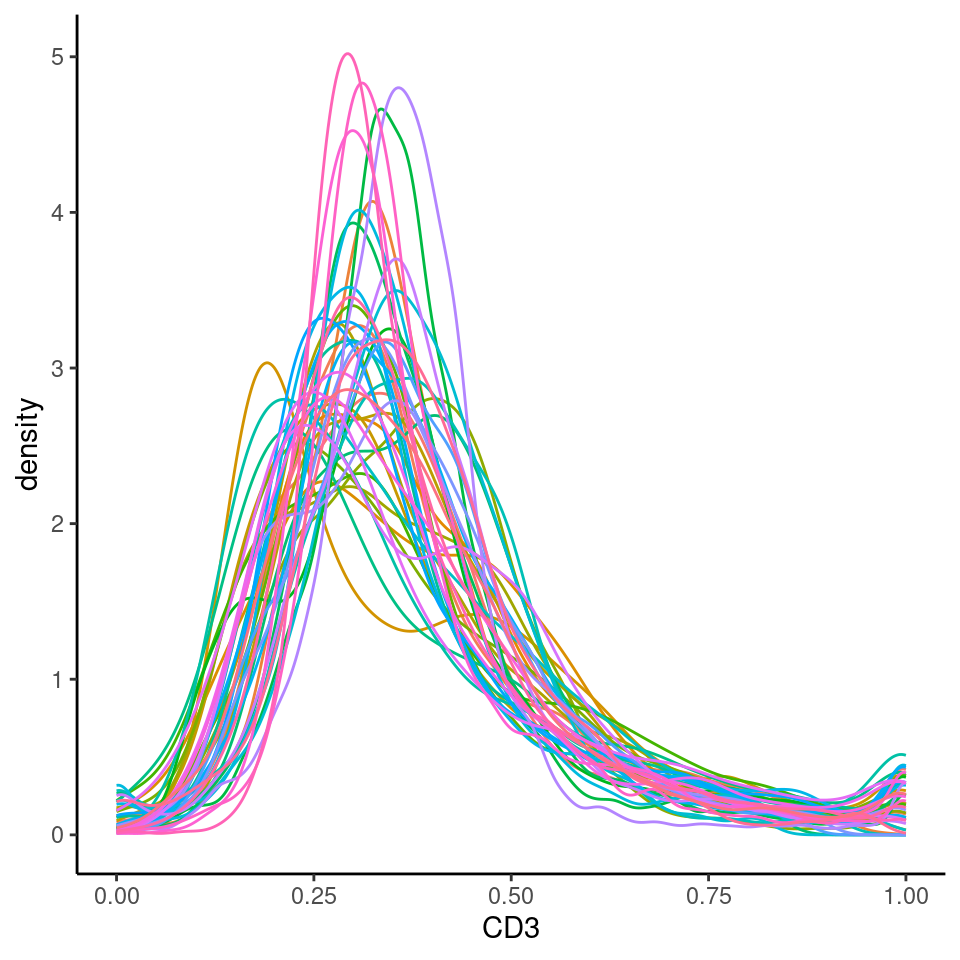
\includegraphics[keepaspectratio]{08-case_study1_files/figure-pdf/unnamed-chunk-14-1.pdf}}

We can also appreciate through the UMAP a reduction of the batch effect
we initially saw.

\begin{Shaded}
\begin{Highlighting}[]
\FunctionTok{set.seed}\NormalTok{(}\DecValTok{51773}\NormalTok{)}
\CommentTok{\# Perform dimension reduction using UMAP.}
\NormalTok{cells }\OtherTok{\textless{}{-}}\NormalTok{ scater}\SpecialCharTok{::}\FunctionTok{runUMAP}\NormalTok{(}
\NormalTok{  cells,}
  \AttributeTok{subset\_row =}\NormalTok{ ct\_markers,}
  \AttributeTok{exprs\_values =} \StringTok{"norm"}\NormalTok{,}
  \AttributeTok{name =} \StringTok{"normUMAP"}
\NormalTok{)}

\NormalTok{someImages }\OtherTok{\textless{}{-}} \FunctionTok{unique}\NormalTok{(cells}\SpecialCharTok{$}\NormalTok{imageID)[}\FunctionTok{c}\NormalTok{(}\DecValTok{1}\NormalTok{, }\DecValTok{5}\NormalTok{, }\DecValTok{10}\NormalTok{, }\DecValTok{20}\NormalTok{, }\DecValTok{30}\NormalTok{, }\DecValTok{40}\NormalTok{)]}

\CommentTok{\# UMAP by imageID.}
\NormalTok{scater}\SpecialCharTok{::}\FunctionTok{plotReducedDim}\NormalTok{(}
\NormalTok{  cells[, cells}\SpecialCharTok{$}\NormalTok{imageID }\SpecialCharTok{\%in\%}\NormalTok{ someImages],}
  \AttributeTok{dimred =} \StringTok{"normUMAP"}\NormalTok{,}
  \AttributeTok{colour\_by =} \StringTok{"imageID"}
\NormalTok{)}
\end{Highlighting}
\end{Shaded}

\pandocbounded{\includegraphics[keepaspectratio]{08-case_study1_files/figure-pdf/unnamed-chunk-15-1.pdf}}

\section{FuseSOM: Cluster cells into cell
types}\label{fusesom-cluster-cells-into-cell-types}

We can appreciate from the UMAP that there is a division of clusters,
most likely representing different cell types. We next aim to
empirically distinguish each cluster using our FuseSOM package for
clustering.

Our FuseSOM R package can be found on bioconductor at
\url{https://www.bioconductor.org/packages/release/bioc/html/FuseSOM.html},
and provides a pipeline for the clustering of highly multiplexed in situ
imaging cytometry assays. This pipeline uses the Self Organising Map
architecture coupled with Multiview hierarchical clustering and provides
functions for the estimation of the number of clusters.

Here we cluster using the \texttt{runFuseSOM} function. We specify the
number of clusters to identify to be \texttt{numClusters\ =\ 10}. We
also specify a set of cell-type specific markers to use, as we want our
clusters to be distinct based off cell type markers, rather than markers
which might pick up a transitioning cell state.

\subsection{Perform the clustering}\label{perform-the-clustering}

\begin{Shaded}
\begin{Highlighting}[]
\CommentTok{\# Set seed.}
\FunctionTok{set.seed}\NormalTok{(}\DecValTok{51773}\NormalTok{)}

\CommentTok{\# Generate SOM and cluster cells into 10 groups}
\NormalTok{cells }\OtherTok{\textless{}{-}} \FunctionTok{runFuseSOM}\NormalTok{(}
\NormalTok{  cells,}
  \AttributeTok{markers =}\NormalTok{ ct\_markers,}
  \AttributeTok{assay =} \StringTok{"norm"}\NormalTok{,}
  \AttributeTok{numClusters =} \DecValTok{10}
\NormalTok{)}
\end{Highlighting}
\end{Shaded}

\begin{verbatim}
You have provided a dataset of class SpatialExperiment
\end{verbatim}

\begin{verbatim}
Everything looks good. Now running the FuseSOM algorithm
\end{verbatim}

\begin{verbatim}
Now Generating the Self Organizing Map Grid
\end{verbatim}

\begin{verbatim}
Optimal Grid Size is: 8
\end{verbatim}

\begin{verbatim}
Now Running the Self Organizing Map Model
\end{verbatim}

\begin{verbatim}
Now Clustering the Prototypes
\end{verbatim}

\begin{verbatim}
Loading required namespace: fastcluster
\end{verbatim}

\begin{verbatim}
Now Mapping Clusters to the Original Data
\end{verbatim}

\begin{verbatim}
The Prototypes have been Clustered and Mapped Successfully
\end{verbatim}

\begin{verbatim}
The FuseSOM algorithm has completed successfully
\end{verbatim}

We can also observe how reasonable our choice of \texttt{k\ =\ 10} was,
using the \texttt{estimateNumCluster()} and \texttt{optiPlot()}
functions. Here we examine the Gap method, but others such as Silhouette
and Within Cluster Distance are also available. We can see that there
are elbow points in the gap statistic at \texttt{k\ =\ 7},
\texttt{k\ =\ 10}, and \texttt{k\ =\ 11}. We've specified
\texttt{k\ =\ 10}, striking a good balance between the number of
clusters and the gap statistic.

\begin{Shaded}
\begin{Highlighting}[]
\NormalTok{cells }\OtherTok{\textless{}{-}} \FunctionTok{estimateNumCluster}\NormalTok{(cells, }\AttributeTok{kSeq =} \DecValTok{2}\SpecialCharTok{:}\DecValTok{30}\NormalTok{)}
\end{Highlighting}
\end{Shaded}

\begin{verbatim}
You have provided a dataset of class: SpatialExperiment
\end{verbatim}

\begin{verbatim}
Now Computing the Number of Clusters using Discriminant Analysis
\end{verbatim}

\begin{verbatim}
Now Computing The Number Of Clusters Using Distance Analysis
\end{verbatim}

\begin{Shaded}
\begin{Highlighting}[]
\FunctionTok{optiPlot}\NormalTok{(cells, }\AttributeTok{method =} \StringTok{"gap"}\NormalTok{)}
\end{Highlighting}
\end{Shaded}

\begin{verbatim}
You have provided a dataset of class: SpatialExperiment
\end{verbatim}

\pandocbounded{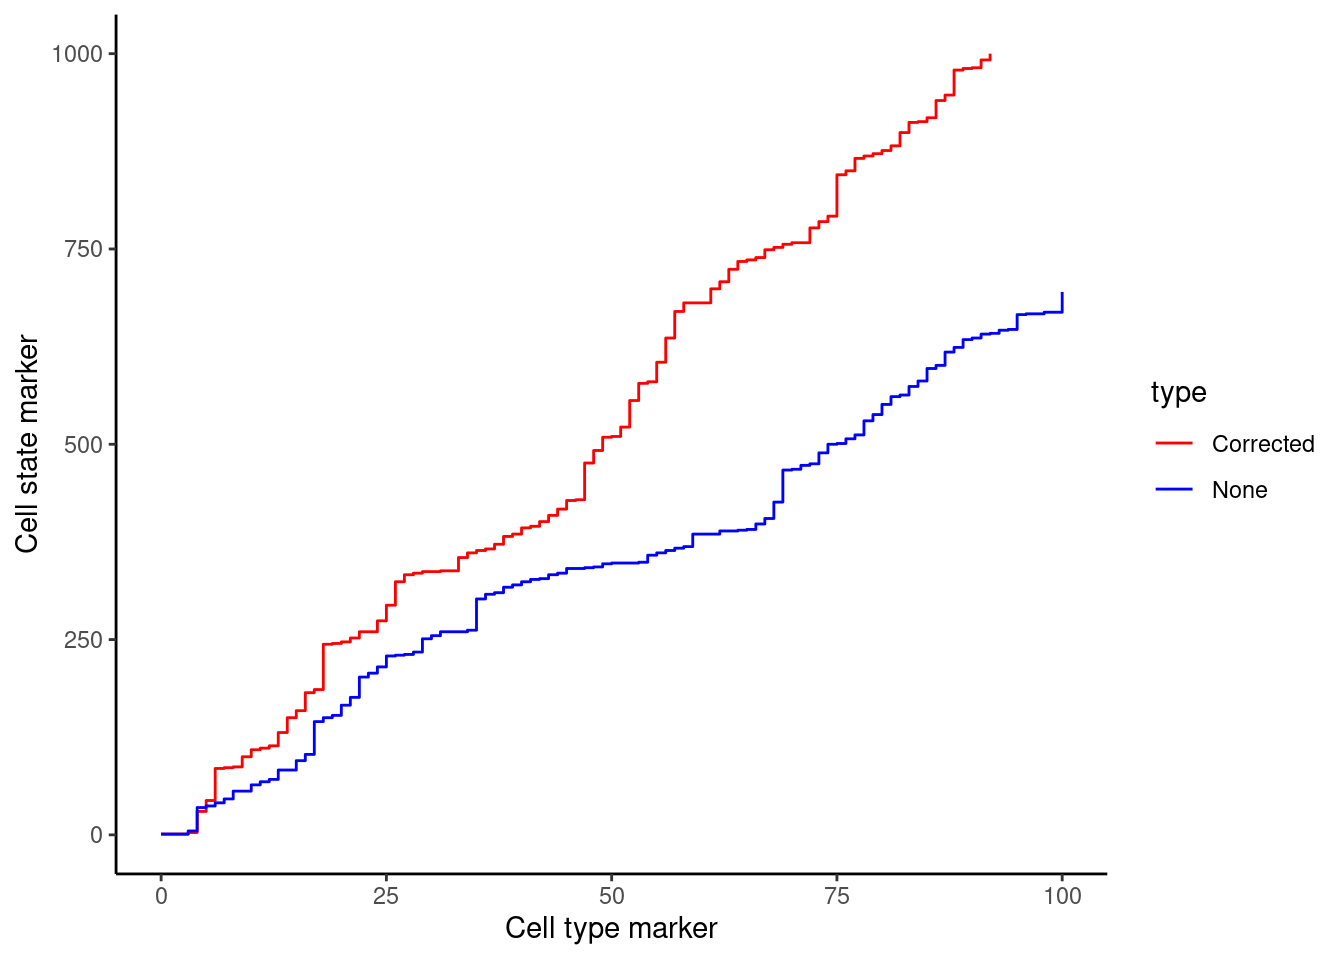
\includegraphics[keepaspectratio]{08-case_study1_files/figure-pdf/unnamed-chunk-16-1.pdf}}

\subsection{Attempt to interpret the phenotype of each
cluster}\label{attempt-to-interpret-the-phenotype-of-each-cluster}

We can begin the process of understanding what each of these cell
clusters are by using the \texttt{plotGroupedHeatmap} function from
\texttt{scater}. At the least, here we can see we capture all the major
immune populations that we expect to see, including the CD4 and CD8 T
cells, the CD20+ B cells, the CD68+ myeloid populations, the CD66+
granulocytes, the podoplanin+ epithelial cells, and the panCK+ tumour
cells.

\begin{Shaded}
\begin{Highlighting}[]
\CommentTok{\# Visualise marker expression in each cluster.}
\NormalTok{scater}\SpecialCharTok{::}\FunctionTok{plotGroupedHeatmap}\NormalTok{(}
\NormalTok{  cells,}
  \AttributeTok{features =}\NormalTok{ ct\_markers,}
  \AttributeTok{group =} \StringTok{"clusters"}\NormalTok{,}
  \AttributeTok{exprs\_values =} \StringTok{"norm"}\NormalTok{,}
  \AttributeTok{center =} \ConstantTok{TRUE}\NormalTok{,}
  \AttributeTok{scale =} \ConstantTok{TRUE}\NormalTok{,}
  \AttributeTok{zlim =} \FunctionTok{c}\NormalTok{(}\SpecialCharTok{{-}}\DecValTok{3}\NormalTok{, }\DecValTok{3}\NormalTok{),}
  \AttributeTok{cluster\_rows =} \ConstantTok{FALSE}\NormalTok{,}
  \AttributeTok{block =} \StringTok{"clusters"}
\NormalTok{)}
\end{Highlighting}
\end{Shaded}

\pandocbounded{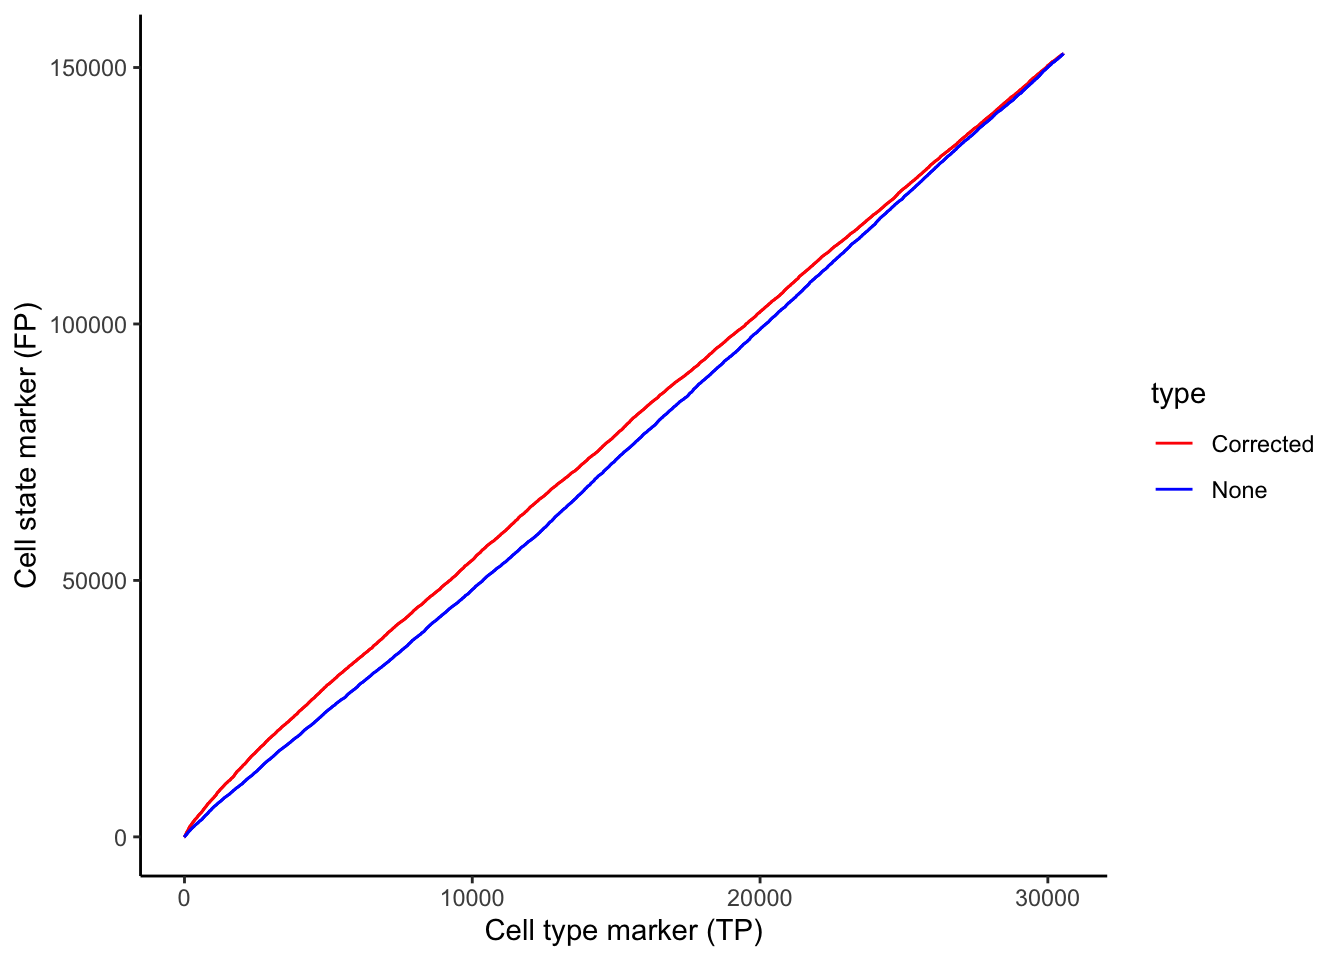
\includegraphics[keepaspectratio]{08-case_study1_files/figure-pdf/unnamed-chunk-17-1.pdf}}

Given domain-specific knowledge of the tumour-immune landscape, we can
go ahead and annotate these clusters as cell types given their
expression profiles.

\begin{Shaded}
\begin{Highlighting}[]
\NormalTok{cells }\OtherTok{\textless{}{-}}\NormalTok{ cells }\SpecialCharTok{|\textgreater{}}
  \FunctionTok{mutate}\NormalTok{(}\AttributeTok{cellType =} \FunctionTok{case\_when}\NormalTok{(}
\NormalTok{    clusters }\SpecialCharTok{==} \StringTok{"cluster\_1"} \SpecialCharTok{\textasciitilde{}} \StringTok{"GC"}\NormalTok{, }\CommentTok{\# Granulocytes}
\NormalTok{    clusters }\SpecialCharTok{==} \StringTok{"cluster\_2"} \SpecialCharTok{\textasciitilde{}} \StringTok{"MC"}\NormalTok{, }\CommentTok{\# Myeloid cells}
\NormalTok{    clusters }\SpecialCharTok{==} \StringTok{"cluster\_3"} \SpecialCharTok{\textasciitilde{}} \StringTok{"SC"}\NormalTok{, }\CommentTok{\# Squamous cells}
\NormalTok{    clusters }\SpecialCharTok{==} \StringTok{"cluster\_4"} \SpecialCharTok{\textasciitilde{}} \StringTok{"EP"}\NormalTok{, }\CommentTok{\# Epithelial cells}
\NormalTok{    clusters }\SpecialCharTok{==} \StringTok{"cluster\_5"} \SpecialCharTok{\textasciitilde{}} \StringTok{"SC"}\NormalTok{, }\CommentTok{\# Squamous cells}
\NormalTok{    clusters }\SpecialCharTok{==} \StringTok{"cluster\_6"} \SpecialCharTok{\textasciitilde{}} \StringTok{"TC\_CD4"}\NormalTok{, }\CommentTok{\# CD4 T cells}
\NormalTok{    clusters }\SpecialCharTok{==} \StringTok{"cluster\_7"} \SpecialCharTok{\textasciitilde{}} \StringTok{"BC"}\NormalTok{, }\CommentTok{\# B cells}
\NormalTok{    clusters }\SpecialCharTok{==} \StringTok{"cluster\_8"} \SpecialCharTok{\textasciitilde{}} \StringTok{"EC"}\NormalTok{, }\CommentTok{\# Endothelial cells}
\NormalTok{    clusters }\SpecialCharTok{==} \StringTok{"cluster\_9"} \SpecialCharTok{\textasciitilde{}} \StringTok{"TC\_CD8"}\NormalTok{, }\CommentTok{\# CD8 T cells}
\NormalTok{    clusters }\SpecialCharTok{==} \StringTok{"cluster\_10"} \SpecialCharTok{\textasciitilde{}} \StringTok{"DC"} \CommentTok{\# Dendritic cells}
\NormalTok{  ))}
\end{Highlighting}
\end{Shaded}

\begin{verbatim}
New names:
New names:
* `UMAP1` -> `UMAP1...1`
* `UMAP2` -> `UMAP2...2`
* `UMAP1` -> `UMAP1...3`
* `UMAP2` -> `UMAP2...4`
\end{verbatim}

We might also be interested in how these cell types are distributed on
the images themselves. Here we examine the distribution of clusters on
image F3, noting the healthy epithelial and endothelial structures
surrounded by tumour cells.

\begin{Shaded}
\begin{Highlighting}[]
\FunctionTok{reducedDim}\NormalTok{(cells, }\StringTok{"spatialCoords"}\NormalTok{) }\OtherTok{\textless{}{-}} \FunctionTok{spatialCoords}\NormalTok{(cells)}

\NormalTok{cells }\SpecialCharTok{|\textgreater{}} 
  \FunctionTok{filter}\NormalTok{(imageID }\SpecialCharTok{==} \StringTok{"F3"}\NormalTok{) }\SpecialCharTok{|\textgreater{}} 
  \FunctionTok{plotReducedDim}\NormalTok{(}\StringTok{"spatialCoords"}\NormalTok{, }\AttributeTok{colour\_by =} \StringTok{"cellType"}\NormalTok{)}
\end{Highlighting}
\end{Shaded}

\begin{verbatim}
New names:
* `UMAP1` -> `UMAP1...1`
* `UMAP2` -> `UMAP2...2`
* `UMAP1` -> `UMAP1...3`
* `UMAP2` -> `UMAP2...4`
\end{verbatim}

\pandocbounded{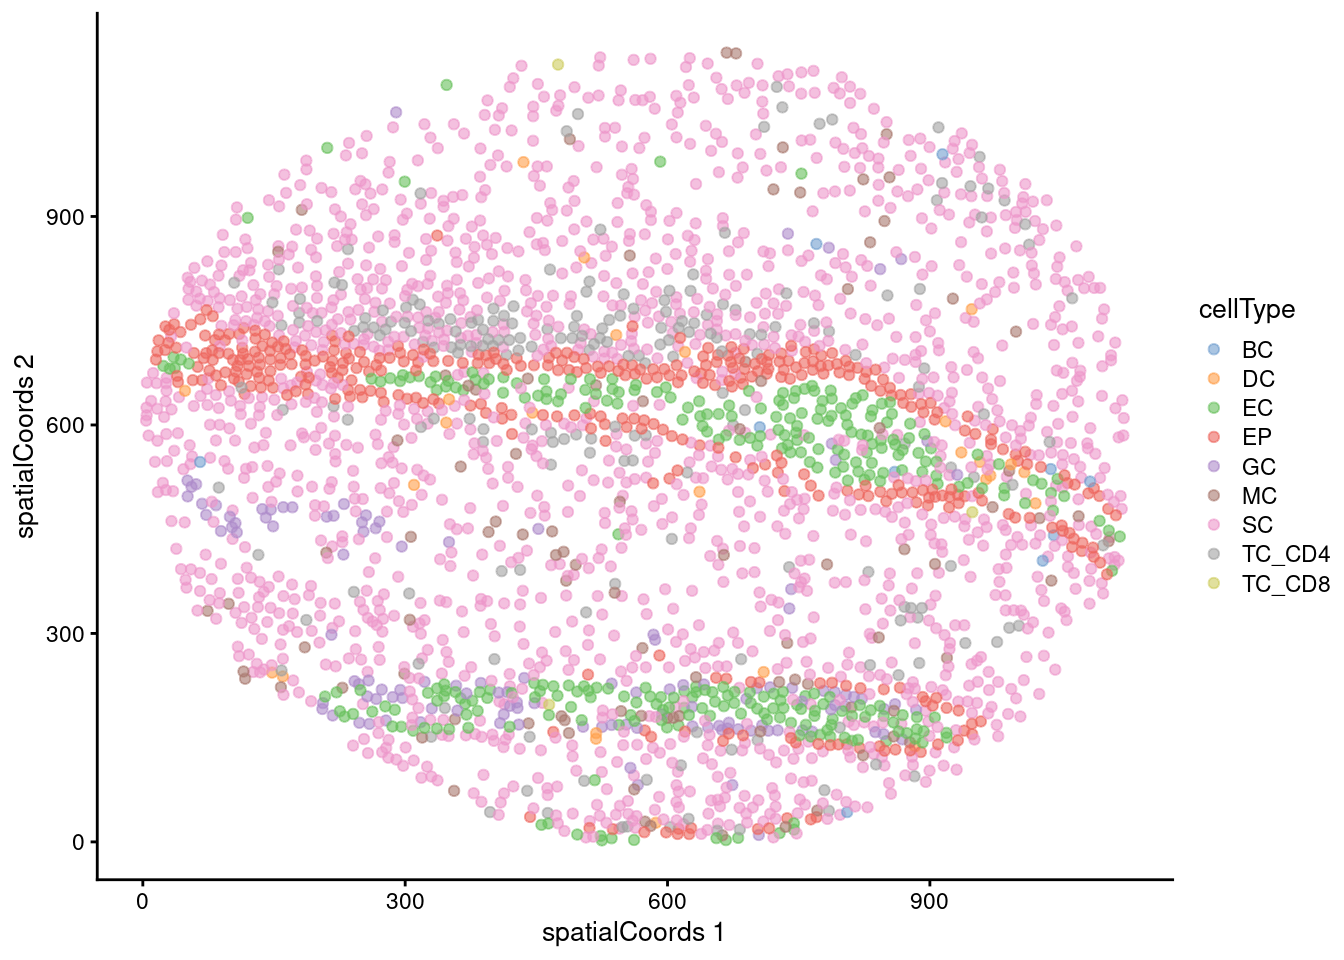
\includegraphics[keepaspectratio]{08-case_study1_files/figure-pdf/unnamed-chunk-19-1.pdf}}

\subsection{Check cell type
frequencies}\label{check-cell-type-frequencies}

We find it always useful to check the number of cells in each cluster.
Here we can see that cluster 10 contains lots of (most likely tumour -
high expression of panCK and non-consistent expression of other markers)
cells and cluster 4 contains very few cells.

\begin{Shaded}
\begin{Highlighting}[]
\CommentTok{\# Check cell type frequencies.}
\NormalTok{cells}\SpecialCharTok{$}\NormalTok{cellType }\SpecialCharTok{|\textgreater{}}
  \FunctionTok{table}\NormalTok{() }\SpecialCharTok{|\textgreater{}}
  \FunctionTok{sort}\NormalTok{()}
\end{Highlighting}
\end{Shaded}

\begin{verbatim}

    DC     BC     MC     GC TC_CD8 TC_CD4     EC     EP     SC 
  2411   4322   5283   7993   8534  11753  14159  14170  87288 
\end{verbatim}

We can also use the UMAP we computed earlier to visualise our data in a
lower dimension and see how well our annotated cell types cluster out.

\begin{Shaded}
\begin{Highlighting}[]
\CommentTok{\# UMAP by cell type}
\NormalTok{scater}\SpecialCharTok{::}\FunctionTok{plotReducedDim}\NormalTok{(}
\NormalTok{  cells[, cells}\SpecialCharTok{$}\NormalTok{imageID }\SpecialCharTok{\%in\%}\NormalTok{ someImages],}
  \AttributeTok{dimred =} \StringTok{"normUMAP"}\NormalTok{,}
  \AttributeTok{colour\_by =} \StringTok{"cellType"}
\NormalTok{)}
\end{Highlighting}
\end{Shaded}

\pandocbounded{\includegraphics[keepaspectratio]{08-case_study1_files/figure-pdf/unnamed-chunk-21-1.pdf}}

\subsection{Testing for association between the proportion of each cell
type and progressor
status}\label{testing-for-association-between-the-proportion-of-each-cell-type-and-progressor-status}

We recommend using a package such as \texttt{diffcyt} for testing for
changes in abundance of cell types. However, the \texttt{colTest}
function allows us to quickly test for associations between the
proportions of the cell types and progression status using either
Wilcoxon rank sum tests or t-tests. Here we see a p-value less than
0.05, but this does not equate to a small FDR.

\begin{Shaded}
\begin{Highlighting}[]
\CommentTok{\# Perform simple student\textquotesingle{}s t{-}tests on the columns of the proportion matrix.}
\NormalTok{testProp }\OtherTok{\textless{}{-}} \FunctionTok{colTest}\NormalTok{(cells, }
                    \AttributeTok{condition =} \StringTok{"group"}\NormalTok{, }
                    \AttributeTok{feature =} \StringTok{"cellType"}\NormalTok{,}
                    \AttributeTok{type =} \StringTok{"ttest"}\NormalTok{)}

\FunctionTok{head}\NormalTok{(testProp)}
\end{Highlighting}
\end{Shaded}

\begin{verbatim}
       mean in group NP mean in group P tval.t  pval adjPval cluster
TC_CD8            0.056           0.033   2.70 0.011   0.099  TC_CD8
MC                0.033           0.040  -1.70 0.099   0.400      MC
EC                0.098           0.085   1.50 0.160   0.400      EC
BC                0.026           0.016   1.30 0.190   0.400      BC
SC                0.560           0.590  -1.30 0.220   0.400      SC
TC_CD4            0.074           0.084  -0.94 0.360   0.540  TC_CD4
\end{verbatim}

Let's examine one of these clusters using our \texttt{getProp()}
function from \texttt{spicyR}, which conveniently transforms our
proportions into a feature matrix of images by cell type, enabling
convenient downstream classification or analysis.

Next, let's visualise how different the proportions are

boxplot.

\begin{Shaded}
\begin{Highlighting}[]
\NormalTok{prop }\OtherTok{\textless{}{-}} \FunctionTok{getProp}\NormalTok{(cells, }\AttributeTok{feature =} \StringTok{"cellType"}\NormalTok{)}
\NormalTok{prop[}\DecValTok{1}\SpecialCharTok{:}\DecValTok{5}\NormalTok{, }\DecValTok{1}\SpecialCharTok{:}\DecValTok{5}\NormalTok{]}
\end{Highlighting}
\end{Shaded}

\begin{verbatim}
           BC         DC         EC         EP          GC
A2 0.01501502 0.00000000 0.09129129 0.04684685 0.031831832
A3 0.01854193 0.00000000 0.09334176 0.01769912 0.001474926
A4 0.01196581 0.00322887 0.07901235 0.02792023 0.003988604
A5 0.02135513 0.03190087 0.07882942 0.15344055 0.140522014
A6 0.01783492 0.01824969 0.08710079 0.14765657 0.125259229
\end{verbatim}

It appears that the CD8 T cells are the most differentially abundant
cell type across our progressors and non-progressors. A boxplot
visualisation of CD8 T cell proportion clearly shows that progressors
have a lower proportion of CD8 T cells in the tumour core.

\begin{Shaded}
\begin{Highlighting}[]
\NormalTok{clusterToUse }\OtherTok{\textless{}{-}} \FunctionTok{rownames}\NormalTok{(testProp)[}\DecValTok{1}\NormalTok{]}

\NormalTok{prop }\SpecialCharTok{|\textgreater{}}
  \FunctionTok{select}\NormalTok{(}\FunctionTok{all\_of}\NormalTok{(clusterToUse)) }\SpecialCharTok{|\textgreater{}}
\NormalTok{  tibble}\SpecialCharTok{::}\FunctionTok{rownames\_to\_column}\NormalTok{(}\StringTok{"imageID"}\NormalTok{) }\SpecialCharTok{|\textgreater{}}
  \FunctionTok{left\_join}\NormalTok{(clinical, }\AttributeTok{by =} \StringTok{"imageID"}\NormalTok{) }\SpecialCharTok{|\textgreater{}}
  \FunctionTok{ggplot}\NormalTok{(}\FunctionTok{aes}\NormalTok{(}\AttributeTok{x =}\NormalTok{ group, }\AttributeTok{y =}\NormalTok{ .data[[clusterToUse]], }\AttributeTok{fill =}\NormalTok{ group)) }\SpecialCharTok{+}
  \FunctionTok{geom\_boxplot}\NormalTok{()}
\end{Highlighting}
\end{Shaded}

\pandocbounded{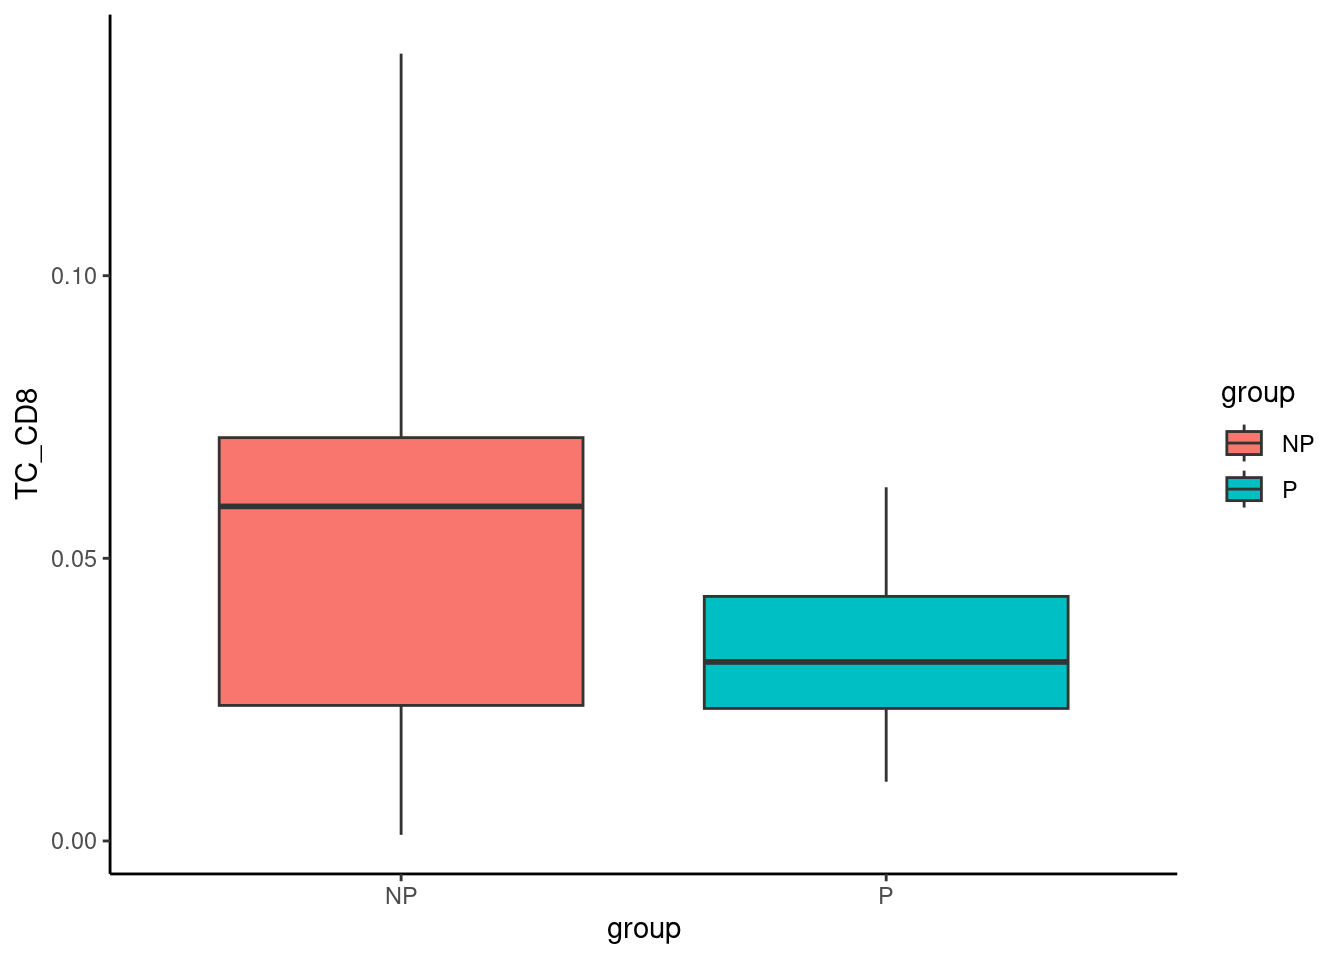
\includegraphics[keepaspectratio]{08-case_study1_files/figure-pdf/unnamed-chunk-24-1.pdf}}

\textbf{NB}: If you have already clustered and annotated your cells, you
may only be interested in our downstream analysis capabilities, looking
into identifying localisation (spicyR), cell regions (lisaClust), and
cell-cell interactions (SpatioMark \& Kontextual). Therefore, for the
sake of convenience, we've provided capability to directly load in the
SpatialExperiment (SPE) object that we've generated up to this point,
complete with clusters and normalised intensities.

\begin{Shaded}
\begin{Highlighting}[]
\FunctionTok{load}\NormalTok{(}\FunctionTok{system.file}\NormalTok{(}\StringTok{"extdata/computed\_cells.rda"}\NormalTok{, }\AttributeTok{package =} \StringTok{"spicyWorkflow"}\NormalTok{))}
\end{Highlighting}
\end{Shaded}

\section{spicyR: Test spatial
relationships}\label{spicyr-test-spatial-relationships}

Our spicyR package is available on bioconductor on
\url{https://www.bioconductor.org/packages/devel/bioc/html/spicyR.html}
and provides a series of functions to aid in the analysis of both
immunofluorescence and imaging mass cytometry data as well as other
assays that can deeply phenotype individual cells and their spatial
location. Here we use the \texttt{spicy()} function to test for changes
in the spatial relationships between pair-wise combinations of cells.

Put simply, spicyR uses the L-function to determine localisation or
dispersion between cell types. The L-function is an arbitrary measure of
``closeness'' between points, with greater values suggesting increased
localisation, and lower values suggesting dispersion.

Here, we quantify spatial relationships using a combination of 10 radii
from 10 to 100 by specifying \texttt{Rs\ =\ 1:10*10} and mildly account
for some global tissue structure using \texttt{sigma\ =\ 50}. Further
information on how to optimise these parameters can be found in the
\href{https://bioconductor.org/packages/release/bioc/vignettes/spicyR/inst/doc/spicyR.html}{vignette}
and the spicyR
\href{https://doi.org/10.1093/bioinformatics/btac268}{paper}.

\begin{Shaded}
\begin{Highlighting}[]
\NormalTok{spicyTest }\OtherTok{\textless{}{-}} \FunctionTok{spicy}\NormalTok{(cells,}
                   \AttributeTok{condition =} \StringTok{"group"}\NormalTok{,}
                   \AttributeTok{cellTypeCol =} \StringTok{"cellType"}\NormalTok{,}
                   \AttributeTok{imageIDCol =} \StringTok{"imageID"}\NormalTok{,}
                   \AttributeTok{Rs =} \DecValTok{1}\SpecialCharTok{:}\DecValTok{10}\SpecialCharTok{*}\DecValTok{10}\NormalTok{,}
                   \AttributeTok{sigma =} \DecValTok{50}\NormalTok{,}
                   \AttributeTok{BPPARAM =}\NormalTok{ BPPARAM)}
\end{Highlighting}
\end{Shaded}

\begin{verbatim}
Coercing condition into factor. Using group = NP as base comparison group. If
this is not the desired base group, please convert cells$group into a factor
and change the order of levels(cells$group) so that the base group is at index
1.
\end{verbatim}

\begin{Shaded}
\begin{Highlighting}[]
\FunctionTok{topPairs}\NormalTok{(spicyTest, }\AttributeTok{n =} \DecValTok{10}\NormalTok{)}
\end{Highlighting}
\end{Shaded}

\begin{verbatim}
            intercept coefficient    p.value adj.pvalue   from     to
BC__EC     -1.1346644    8.304020 0.03391529  0.6931721     BC     EC
EC__BC     -1.5909700    7.919971 0.04134661  0.6931721     EC     BC
GC__TC_CD4 -7.6316673   11.005639 0.05047096  0.6931721     GC TC_CD4
TC_CD4__GC -7.5406782   11.077602 0.05709461  0.6931721 TC_CD4     GC
TC_CD4__EP -0.7117393    4.853317 0.07261120  0.6931721 TC_CD4     EP
EP__TC_CD4 -0.7070918    4.820661 0.07510118  0.6931721     EP TC_CD4
EP__TC_CD8 -3.1445464    5.779536 0.08047994  0.6931721     EP TC_CD8
TC_CD8__EP -2.9313474    5.688420 0.09522058  0.6931721 TC_CD8     EP
TC_CD4__EC  3.1984391    4.366122 0.09716499  0.6931721 TC_CD4     EC
EC__TC_CD4  3.1052061    4.263971 0.10461424  0.6931721     EC TC_CD4
\end{verbatim}

We can visualise these tests using \texttt{signifPlot} where we observe
that cell type pairs appear to become less attractive (or avoid more) in
the progression sample.

\begin{Shaded}
\begin{Highlighting}[]
\CommentTok{\# Visualise which relationships are changing the most.}
\FunctionTok{signifPlot}\NormalTok{(}
\NormalTok{  spicyTest,}
  \AttributeTok{breaks =} \FunctionTok{c}\NormalTok{(}\SpecialCharTok{{-}}\FloatTok{1.5}\NormalTok{, }\FloatTok{1.5}\NormalTok{, }\FloatTok{0.5}\NormalTok{)}
\NormalTok{)}
\end{Highlighting}
\end{Shaded}

\pandocbounded{\includegraphics[keepaspectratio]{08-case_study1_files/figure-pdf/unnamed-chunk-27-1.pdf}}

\texttt{spicyR} also has functionality for plotting out individual
pairwise relationships. We can first try look into whether the
\texttt{SC} tumour cell type localises with the \texttt{GC} granular
cell type, and whether this localisation affects progression vs
non-progression of the tumour.

\begin{Shaded}
\begin{Highlighting}[]
\FunctionTok{spicyBoxPlot}\NormalTok{(spicyTest, }
             \AttributeTok{from =} \StringTok{"SC"}\NormalTok{, }
             \AttributeTok{to =} \StringTok{"GC"}\NormalTok{)}
\end{Highlighting}
\end{Shaded}

\begin{verbatim}
Warning: Removed 1 row containing non-finite outside the scale range
(`stat_boxplot()`).
\end{verbatim}

\pandocbounded{\includegraphics[keepaspectratio]{08-case_study1_files/figure-pdf/unnamed-chunk-28-1.pdf}}

Alternatively, we can look at the most differentially localised
relationship between progressors and non-progressors by specifying
\texttt{rank\ =\ 1}.

\begin{Shaded}
\begin{Highlighting}[]
\FunctionTok{spicyBoxPlot}\NormalTok{(spicyTest, }
             \AttributeTok{rank =} \DecValTok{1}\NormalTok{)}
\end{Highlighting}
\end{Shaded}

\pandocbounded{\includegraphics[keepaspectratio]{08-case_study1_files/figure-pdf/unnamed-chunk-29-1.pdf}}

\section{lisaClust: Find cellular
neighbourhoods}\label{lisaclust-find-cellular-neighbourhoods}

Our lisaClust package
(https://www.bioconductor.org/packages/devel/bioc/html/lisaClust.html){[}https://www.bioconductor.org/packages/devel/bioc/html/lisaClust.html{]}
provides a series of functions to identify and visualise regions of
tissue where spatial associations between cell-types is similar. This
package can be used to provide a high-level summary of cell-type
co-localisation in multiplexed imaging data that has been segmented at a
single-cell resolution. Here we use the \texttt{lisaClust} function to
clusters cells into 5 regions with distinct spatial ordering.

\begin{Shaded}
\begin{Highlighting}[]
\FunctionTok{set.seed}\NormalTok{(}\DecValTok{51773}\NormalTok{)}

\CommentTok{\# Cluster cells into spatial regions with similar composition.}
\NormalTok{cells }\OtherTok{\textless{}{-}} \FunctionTok{lisaClust}\NormalTok{(}
\NormalTok{  cells,}
  \AttributeTok{k =} \DecValTok{4}\NormalTok{,}
  \AttributeTok{sigma =} \DecValTok{50}\NormalTok{,}
  \AttributeTok{cellType =} \StringTok{"cellType"}\NormalTok{,}
  \AttributeTok{BPPARAM =}\NormalTok{ BPPARAM}
\NormalTok{)}
\end{Highlighting}
\end{Shaded}

\begin{verbatim}
Generating local L-curves.
\end{verbatim}

\subsection{Region - cell type enrichment
heatmap}\label{region---cell-type-enrichment-heatmap}

We can try to interpret which spatial orderings the regions are
quantifying using the \texttt{regionMap} function. This plots the
frequency of each cell type in a region relative to what you would
expect by chance. We can see here that our regions have neatly separated
according to biological milieu, with region 1 and 2 representing our
immune cell regions, region 3 representing our tumour cells, and region
4 representing our healthy epithelial and endothelial cells.

\begin{Shaded}
\begin{Highlighting}[]
\CommentTok{\# Visualise the enrichment of each cell type in each region}
\FunctionTok{regionMap}\NormalTok{(cells, }\AttributeTok{cellType =} \StringTok{"cellType"}\NormalTok{, }\AttributeTok{limit =} \FunctionTok{c}\NormalTok{(}\FloatTok{0.2}\NormalTok{, }\DecValTok{2}\NormalTok{))}
\end{Highlighting}
\end{Shaded}

\pandocbounded{\includegraphics[keepaspectratio]{08-case_study1_files/figure-pdf/unnamed-chunk-31-1.pdf}}

\subsection{Visualise regions}\label{visualise-regions}

By default, these identified regions are stored in the \texttt{regions}
column in the \texttt{colData} of our object. We can quickly examine the
spatial arrangement of these regions using \texttt{ggplot} on image F3,
where we can see the same division of immune, healthy, and tumour tissue
that we identified in our \texttt{regionMap}.

\begin{Shaded}
\begin{Highlighting}[]
\NormalTok{cells }\SpecialCharTok{|\textgreater{}} 
  \FunctionTok{filter}\NormalTok{(imageID }\SpecialCharTok{==} \StringTok{"F3"}\NormalTok{) }\SpecialCharTok{|\textgreater{}} 
  \FunctionTok{plotReducedDim}\NormalTok{(}\StringTok{"spatialCoords"}\NormalTok{, }\AttributeTok{colour\_by =} \StringTok{"region"}\NormalTok{)}
\end{Highlighting}
\end{Shaded}

\pandocbounded{\includegraphics[keepaspectratio]{08-case_study1_files/figure-pdf/unnamed-chunk-32-1.pdf}}

While much slower, we have also implemented a function for overlaying
the region information as a hatching pattern so that the information can
be viewed simultaneously with the cell type calls.

\begin{Shaded}
\begin{Highlighting}[]
\CommentTok{\# Use hatching to visualise regions and cell types.}
\FunctionTok{hatchingPlot}\NormalTok{(}
\NormalTok{  cells,}
  \AttributeTok{useImages =} \StringTok{"F3"}\NormalTok{,}
  \AttributeTok{cellType =} \StringTok{"cellType"}\NormalTok{,}
  \AttributeTok{nbp =} \DecValTok{300}
\NormalTok{)}
\end{Highlighting}
\end{Shaded}

\begin{verbatim}
Concave windows are temperamental. Try choosing values of window.length > and < 1 if you have problems.
\end{verbatim}

\pandocbounded{\includegraphics[keepaspectratio]{08-case_study1_files/figure-pdf/unnamed-chunk-33-1.pdf}}

\subsection{Test for association with
progression}\label{test-for-association-with-progression}

Similar to cell type proportions, we can quickly use the
\texttt{colTest} function to test for associations between the
proportions of cells in each region and progression status by specifying
\texttt{feature\ =\ "region"}.

\begin{Shaded}
\begin{Highlighting}[]
\CommentTok{\# Test if the proportion of each region is associated}
\CommentTok{\# with progression status.}
\NormalTok{testRegion }\OtherTok{\textless{}{-}} \FunctionTok{colTest}\NormalTok{(}
\NormalTok{  cells,}
  \AttributeTok{feature =} \StringTok{"region"}\NormalTok{,}
  \AttributeTok{condition =} \StringTok{"group"}\NormalTok{,}
  \AttributeTok{type =} \StringTok{"ttest"}
\NormalTok{)}

\NormalTok{testRegion}
\end{Highlighting}
\end{Shaded}

\begin{verbatim}
         mean in group NP mean in group P tval.t  pval adjPval  cluster
region_1            0.022          0.0079   1.90 0.066    0.20 region_1
region_3            0.092          0.1300  -1.70 0.100    0.20 region_3
region_4            0.340          0.3300   0.63 0.530    0.71 region_4
region_2            0.540          0.5400   0.20 0.840    0.84 region_2
\end{verbatim}

\section{Statial: Identify changes in cell
state.}\label{statial-identify-changes-in-cell-state.}

Our Statial package
(https://www.bioconductor.org/packages/release/bioc/html/Statial.html)
provides a suite of functions (Kontextual) for robust quantification of
cell type localisation which are invariant to changes in tissue
structure. In addition, we provide a suite of functions (SpatioMark) for
uncovering continuous changes in marker expression associated with
varying levels of localisation.

\subsection{SpatioMark: Continuous changes in marker expression
associated with varying levels of
localisation.}\label{spatiomark-continuous-changes-in-marker-expression-associated-with-varying-levels-of-localisation.}

The first step in analysing these changes is to calculate the spatial
proximity (\texttt{getDistances}) of each cell to every cell type. These
values will then be stored in the \texttt{reducedDims} slot of the
\texttt{SingleCellExperiment} object under the names \texttt{distances}.
SpatioMark also provides functionality to look into proximal cell
abundance using the \texttt{getAbundance()} function, which is further
explored within the \texttt{Statial} package vignette.

\begin{Shaded}
\begin{Highlighting}[]
\NormalTok{cells}\SpecialCharTok{$}\NormalTok{m.cx }\OtherTok{\textless{}{-}} \FunctionTok{spatialCoords}\NormalTok{(cells)[,}\StringTok{"x"}\NormalTok{]}
\NormalTok{cells}\SpecialCharTok{$}\NormalTok{m.cy }\OtherTok{\textless{}{-}} \FunctionTok{spatialCoords}\NormalTok{(cells)[,}\StringTok{"y"}\NormalTok{]}

\NormalTok{cells }\OtherTok{\textless{}{-}} \FunctionTok{getDistances}\NormalTok{(cells,}
  \AttributeTok{maxDist =} \DecValTok{200}\NormalTok{,}
  \AttributeTok{nCores =}\NormalTok{ nCores,}
  \AttributeTok{cellType =} \StringTok{"cellType"}\NormalTok{,}
  \AttributeTok{spatialCoords =} \FunctionTok{c}\NormalTok{(}\StringTok{"m.cx"}\NormalTok{, }\StringTok{"m.cy"}\NormalTok{)}
\NormalTok{)}
\end{Highlighting}
\end{Shaded}

We can then visualise an example image, specified with
\texttt{image\ =\ "F3"} and a particular marker interaction with cell
type localisation. To visualise these changes, we specify two cell types
with the \texttt{from} and \texttt{to} parameters, and a marker with the
\texttt{marker} parameter (cell-cell-marker interactions). Here, we
specify the changes in the marker podoplanin in \texttt{SC} tumour cells
as its localisation to \texttt{EP} epithelial cells increases or
decreases, where we can observe that podoplanin decreases in tumour
cells as its distance to the central cluster of epithelial cells
increases.

\begin{Shaded}
\begin{Highlighting}[]
\NormalTok{p }\OtherTok{\textless{}{-}} \FunctionTok{plotStateChanges}\NormalTok{(}
  \AttributeTok{cells =}\NormalTok{ cells,}
  \AttributeTok{cellType =} \StringTok{"cellType"}\NormalTok{,}
  \AttributeTok{spatialCoords =} \FunctionTok{c}\NormalTok{(}\StringTok{"m.cx"}\NormalTok{, }\StringTok{"m.cy"}\NormalTok{),}
  \AttributeTok{type =} \StringTok{"distances"}\NormalTok{,}
  \AttributeTok{image =} \StringTok{"F3"}\NormalTok{,}
  \AttributeTok{from =} \StringTok{"SC"}\NormalTok{,}
  \AttributeTok{to =} \StringTok{"EP"}\NormalTok{,}
  \AttributeTok{marker =} \StringTok{"podoplanin"}\NormalTok{,}
  \AttributeTok{size =} \DecValTok{1}\NormalTok{,}
  \AttributeTok{shape =} \DecValTok{19}\NormalTok{,}
  \AttributeTok{interactive =} \ConstantTok{FALSE}\NormalTok{,}
  \AttributeTok{plotModelFit =} \ConstantTok{FALSE}\NormalTok{,}
  \AttributeTok{method =} \StringTok{"lm"}
\NormalTok{)}

\NormalTok{p}
\end{Highlighting}
\end{Shaded}

\begin{verbatim}
$image
\end{verbatim}

\pandocbounded{\includegraphics[keepaspectratio]{08-case_study1_files/figure-pdf/unnamed-chunk-36-1.pdf}}

\begin{verbatim}

$scatter
\end{verbatim}

\begin{verbatim}
`geom_smooth()` using formula = 'y ~ x'
\end{verbatim}

\pandocbounded{\includegraphics[keepaspectratio]{08-case_study1_files/figure-pdf/unnamed-chunk-36-2.pdf}}

SpatioMark aims to holistically uncover all such significant
relationships by looking at all interactions across all images. The
\texttt{calcStateChanges} function provided by Statial can be expanded
for this exact purpose - by not specifying cell types, a marker, or an
image, \texttt{calcStateChanges} will examine the most significant
correlations between distance and marker expression across the entire
dataset.

\begin{Shaded}
\begin{Highlighting}[]
\NormalTok{state\_dist }\OtherTok{\textless{}{-}} \FunctionTok{calcStateChanges}\NormalTok{(}
  \AttributeTok{cells =}\NormalTok{ cells,}
  \AttributeTok{cellType =} \StringTok{"cellType"}\NormalTok{,}
  \AttributeTok{type =} \StringTok{"distances"}\NormalTok{,}
  \AttributeTok{assay =} \DecValTok{2}\NormalTok{,}
  \AttributeTok{nCores =}\NormalTok{ nCores,}
  \AttributeTok{minCells =} \DecValTok{100}
\NormalTok{)}

\FunctionTok{head}\NormalTok{(state\_dist[state\_dist}\SpecialCharTok{$}\NormalTok{imageID }\SpecialCharTok{==} \StringTok{"F3"}\NormalTok{,], }\AttributeTok{n =} \DecValTok{10}\NormalTok{)}
\end{Highlighting}
\end{Shaded}

\begin{verbatim}
      imageID primaryCellType otherCellType     marker          coef      tval
51990      F3              SC            EP podoplanin -0.0006911103 -16.90036
23703      F3              EP            GC      CXCR3  0.0012103305  15.04988
23704      F3              EP            GC     pSTAT3  0.0012299816  14.79933
51978      F3              SC            GC       PDL2  0.0008802428  13.12601
23669      F3              EP            MC       CCR7  0.0011476888  13.32900
23595      F3              EP        TC_CD8      CXCR3  0.0016741880  12.95156
51981      F3              SC            GC       ICOS  0.0005186181  11.75830
23696      F3              EP            GC      CADM1  0.0011398625  12.18028
11426      F3              EC            GC       CD31  0.0010070252  12.40866
23650      F3              EP            EC       TIM3  0.0033539928  12.05028
              pval          fdr
51990 4.203881e-59 9.004712e-57
23703 8.041089e-41 8.191646e-39
23704 8.916789e-40 8.712976e-38
51978 1.839014e-37 1.637728e-35
23669 9.360248e-34 6.863845e-32
23595 3.025912e-32 2.085497e-30
51981 1.113579e-30 7.070268e-29
23696 3.239532e-29 1.903862e-27
11426 4.839241e-29 2.825645e-27
23650 1.030900e-28 5.930114e-27
\end{verbatim}

The results from our SpatioMark outputs can be converted from a
\texttt{data.frame} to a \texttt{matrix}, using the
\texttt{prepMatrix()} function. Note, the choice of extracting either
the t-statistic or the coefficient of the linear regression can be
specified using the \texttt{column\ =\ "tval"} parameter, with the
coefficient being the default extracted parameter. We can see that with
SpatioMark, we get some features which are significant after adjusting
for FDR.

\begin{Shaded}
\begin{Highlighting}[]
\CommentTok{\# Preparing outcome vector}
\NormalTok{outcome }\OtherTok{\textless{}{-}}\NormalTok{ cells}\SpecialCharTok{$}\NormalTok{group[}\SpecialCharTok{!}\FunctionTok{duplicated}\NormalTok{(cells}\SpecialCharTok{$}\NormalTok{imageID)]}
\FunctionTok{names}\NormalTok{(outcome) }\OtherTok{\textless{}{-}}\NormalTok{ cells}\SpecialCharTok{$}\NormalTok{imageID[}\SpecialCharTok{!}\FunctionTok{duplicated}\NormalTok{(cells}\SpecialCharTok{$}\NormalTok{imageID)]}

\CommentTok{\# Preparing features for Statial}
\NormalTok{distMat }\OtherTok{\textless{}{-}} \FunctionTok{prepMatrix}\NormalTok{(state\_dist)}

\NormalTok{distMat }\OtherTok{\textless{}{-}}\NormalTok{ distMat[}\FunctionTok{names}\NormalTok{(outcome), ]}

\CommentTok{\# Remove some very small values}
\NormalTok{distMat }\OtherTok{\textless{}{-}}\NormalTok{ distMat[, }\FunctionTok{colMeans}\NormalTok{(}\FunctionTok{abs}\NormalTok{(distMat) }\SpecialCharTok{\textgreater{}} \FloatTok{0.0001}\NormalTok{) }\SpecialCharTok{\textgreater{}}\NormalTok{ .}\DecValTok{8}\NormalTok{]}

\NormalTok{survivalResults }\OtherTok{\textless{}{-}} \FunctionTok{colTest}\NormalTok{(distMat, outcome, }\AttributeTok{type =} \StringTok{"ttest"}\NormalTok{)}

\FunctionTok{head}\NormalTok{(survivalResults)}
\end{Highlighting}
\end{Shaded}

\begin{verbatim}
                  mean in group NP mean in group P tval.t    pval adjPval
EC__EC__CD13              -0.00240        -9.6e-04   -3.6 0.00086    0.27
SC__SC__VISTA             -0.00470        -1.7e-03   -3.3 0.00190    0.27
SC__TC_CD4__CXCR3         -0.00015         8.8e-04   -3.4 0.00230    0.27
SC__EP__Ki67              -0.00037        -7.3e-05   -3.2 0.00260    0.27
EC__SC__CD68               0.00029        -3.9e-04    3.2 0.00300    0.27
SC__BC__DNA1               0.02600        -1.4e-01    3.0 0.00480    0.27
                            cluster
EC__EC__CD13           EC__EC__CD13
SC__SC__VISTA         SC__SC__VISTA
SC__TC_CD4__CXCR3 SC__TC_CD4__CXCR3
SC__EP__Ki67           SC__EP__Ki67
EC__SC__CD68           EC__SC__CD68
SC__BC__DNA1           SC__BC__DNA1
\end{verbatim}

\subsection{Kontextual: Robust quantification of cell type localisation
which is invariant to changes in tissue
structure}\label{kontextual-robust-quantification-of-cell-type-localisation-which-is-invariant-to-changes-in-tissue-structure}

\texttt{Kontextual} is a method to evaluate the localisation
relationship between two cell types in an image. \texttt{Kontextual}
builds on the L-function by contextualising the relationship between two
cell types in reference to the typical spatial behaviour of a \(3^{rd}\)
cell type/population. By taking this approach, \texttt{Kontextual} is
invariant to changes in the window of the image as well as tissue
structures which may be present.

The definitions of cell types and cell states are somewhat ambiguous,
cell types imply well defined groups of cells that serve different roles
from one another, on the other hand cell states imply that cells are a
dynamic entity which cannot be discretised, and thus exist in a
continuum. For the purposes of using \texttt{Kontextual} we treat cell
states as identified clusters of cells, where larger clusters represent
a ``parent'' cell population, and finer sub-clusters representing a
``child'' cell population. For example a CD4 T cell may be considered a
child to a larger parent population of Immune cells. \texttt{Kontextual}
thus aims to see how a child population of cells deviate from the
spatial behaviour of their parent population, and how that influences
the localisation between the child cell state and another cell state.

\subsubsection{Cell type hierarchy}\label{cell-type-hierarchy}

A key input for Kontextual is an annotation of cell type hierarchies. We
will need these to organise all the cells present into cell state
populations or clusters, e.g.~all the different B cell types are put in
a vector called bcells.

Here, we use the \texttt{treeKor} bioconductor package
\href{http://www.bioconductor.org/packages/release/bioc/html/treekoR.html}{treekoR}
to define these hierarchies in a data driven way.

\begin{Shaded}
\begin{Highlighting}[]
\NormalTok{fergusonTree }\OtherTok{\textless{}{-}}\NormalTok{ treekoR}\SpecialCharTok{::}\FunctionTok{getClusterTree}\NormalTok{(}\FunctionTok{t}\NormalTok{(}\FunctionTok{assay}\NormalTok{(cells, }\StringTok{"norm"}\NormalTok{)),}
\NormalTok{                                        cells}\SpecialCharTok{$}\NormalTok{cellType,}
                                        \AttributeTok{hierarchy\_method=}\StringTok{"hopach"}\NormalTok{)}

\NormalTok{parent1 }\OtherTok{\textless{}{-}} \FunctionTok{c}\NormalTok{(}\StringTok{"TC\_CD8"}\NormalTok{, }\StringTok{"TC\_CD4"}\NormalTok{, }\StringTok{"DC"}\NormalTok{)}
\NormalTok{parent2 }\OtherTok{\textless{}{-}} \FunctionTok{c}\NormalTok{(}\StringTok{"BC"}\NormalTok{, }\StringTok{"GC"}\NormalTok{)}
\NormalTok{parent3 }\OtherTok{\textless{}{-}} \FunctionTok{c}\NormalTok{(parent1, parent2)}

\NormalTok{parent4 }\OtherTok{\textless{}{-}} \FunctionTok{c}\NormalTok{(}\StringTok{"MC"}\NormalTok{, }\StringTok{"EP"}\NormalTok{, }\StringTok{"SC"}\NormalTok{)}
\NormalTok{parent5 }\OtherTok{\textless{}{-}} \FunctionTok{c}\NormalTok{(parent4, }\StringTok{"EC"}\NormalTok{)}

\NormalTok{all }\OtherTok{=} \FunctionTok{c}\NormalTok{(parent1, parent2, parent3, parent4, parent5)}

\NormalTok{treeDf }\OtherTok{=}\NormalTok{ Statial}\SpecialCharTok{::}\FunctionTok{parentCombinations}\NormalTok{(all, parent1, parent2, parent3, parent4, parent5)}

\NormalTok{fergusonTree}\SpecialCharTok{$}\NormalTok{clust\_tree }\SpecialCharTok{|\textgreater{}} \FunctionTok{plot}\NormalTok{()}
\end{Highlighting}
\end{Shaded}

\pandocbounded{\includegraphics[keepaspectratio]{08-case_study1_files/figure-pdf/unnamed-chunk-39-1.pdf}}

\texttt{Kontextual} accepts a \texttt{SingleCellExperiment} object, a
single image, or list of images from a \texttt{SingleCellExperiment}
object, which gets passed into the \texttt{cells} argument. Here, we've
specified Kontextual to perform calculations on all pairwise
combinations for every cluster using the \texttt{parentCombinations()}
function to create the \texttt{treeDf} dataframe which we've specified
in the \texttt{parentDf} parameter. The argument \texttt{r} will specify
the radius which the cell relationship will be evaluated on.
\texttt{Kontextual} supports parallel processing, the number of cores
can be specified using the \texttt{cores} argument. \texttt{Kontextual}
can take a single value or multiple values for each argument and will
test all combinations of the arguments specified.

We can calculate all pairwise relationships across all images for a
single radius.

\begin{Shaded}
\begin{Highlighting}[]
\NormalTok{kontext }\OtherTok{\textless{}{-}} \FunctionTok{Kontextual}\NormalTok{(}
  \AttributeTok{cells =}\NormalTok{ cells,}
  \AttributeTok{cellType =} \StringTok{"cellType"}\NormalTok{,}
  \AttributeTok{spatialCoords =} \FunctionTok{c}\NormalTok{(}\StringTok{"m.cx"}\NormalTok{, }\StringTok{"m.cy"}\NormalTok{),}
  \AttributeTok{parentDf =}\NormalTok{ treeDf,}
  \AttributeTok{r =} \DecValTok{50}\NormalTok{,}
  \AttributeTok{cores =}\NormalTok{ nCores}
\NormalTok{)}
\end{Highlighting}
\end{Shaded}

Again, we can use the same \texttt{colTest()} to quickly test for
associations between the Kontextual values and progression status using
either Wilcoxon rank sum tests or t-tests. Similar to SpatioMark, we can
specify using either the original L-function by specifying
\texttt{column\ =\ "original"} in our \texttt{prepMatrix()} function.

\begin{Shaded}
\begin{Highlighting}[]
\CommentTok{\# Converting Kontextual result into data matrix}
\NormalTok{kontextMat }\OtherTok{\textless{}{-}} \FunctionTok{prepMatrix}\NormalTok{(kontext)}

\CommentTok{\# Replace NAs with 0}
\NormalTok{kontextMat[}\FunctionTok{is.na}\NormalTok{(kontextMat)] }\OtherTok{\textless{}{-}} \DecValTok{0}

\NormalTok{survivalResults }\OtherTok{\textless{}{-}}\NormalTok{ spicyR}\SpecialCharTok{::}\FunctionTok{colTest}\NormalTok{(kontextMat, outcome, }\AttributeTok{type =} \StringTok{"ttest"}\NormalTok{)}

\FunctionTok{head}\NormalTok{(survivalResults)}
\end{Highlighting}
\end{Shaded}

\begin{verbatim}
                    mean in group NP mean in group P tval.t    pval adjPval
SC__BC__parent2                  4.9           -3.80    3.9 0.00039   0.053
SC__GC__parent3                 -3.7            2.60   -3.4 0.00140   0.095
SC__TC_CD4__parent3              2.9            0.24    2.7 0.00920   0.420
TC_CD4__EC__parent5              4.0           10.00   -2.5 0.01700   0.520
BC__TC_CD8__parent3             -5.5            3.10   -2.2 0.03100   0.520
SC__BC__parent3                  1.1           -3.80    2.2 0.03300   0.520
                                cluster
SC__BC__parent2         SC__BC__parent2
SC__GC__parent3         SC__GC__parent3
SC__TC_CD4__parent3 SC__TC_CD4__parent3
TC_CD4__EC__parent5 TC_CD4__EC__parent5
BC__TC_CD8__parent3 BC__TC_CD8__parent3
SC__BC__parent3         SC__BC__parent3
\end{verbatim}

\section{ClassifyR: Classification}\label{classifyr-classification}

Our ClassifyR package, \url{https://github.com/SydneyBioX/ClassifyR},
formalises a convenient framework for evaluating classification in R. We
provide functionality to easily include four key modelling stages; Data
transformation, feature selection, classifier training and prediction;
into a cross-validation loop. Here we use the \texttt{crossValidate}
function to perform 100 repeats of 5-fold cross-validation to evaluate
the performance of a random forest applied to five quantifications of
our IMC data; 1) Cell type proportions 2) Cell type localisation from
\texttt{spicyR} 3) Region proportions from \texttt{lisaClust} 4) Cell
type localisation in reference to a parent cell type from
\texttt{Kontextual} 5) Cell changes in response to proximal changes from
\texttt{SpatioMark}

\begin{Shaded}
\begin{Highlighting}[]
\CommentTok{\# Create list to store data.frames}
\NormalTok{data }\OtherTok{\textless{}{-}} \FunctionTok{list}\NormalTok{()}

\CommentTok{\# Add proportions of each cell type in each image}
\NormalTok{data[[}\StringTok{"Proportions"}\NormalTok{]] }\OtherTok{\textless{}{-}} \FunctionTok{getProp}\NormalTok{(cells, }\StringTok{"cellType"}\NormalTok{)}

\CommentTok{\# Add pair{-}wise associations}
\NormalTok{spicyMat }\OtherTok{\textless{}{-}} \FunctionTok{bind}\NormalTok{(spicyTest)}
\NormalTok{spicyMat[}\FunctionTok{is.na}\NormalTok{(spicyMat)] }\OtherTok{\textless{}{-}} \DecValTok{0}
\NormalTok{spicyMat }\OtherTok{\textless{}{-}}\NormalTok{ spicyMat }\SpecialCharTok{|\textgreater{}}
  \FunctionTok{select}\NormalTok{(}\SpecialCharTok{!}\NormalTok{condition) }\SpecialCharTok{|\textgreater{}}
\NormalTok{  tibble}\SpecialCharTok{::}\FunctionTok{column\_to\_rownames}\NormalTok{(}\StringTok{"imageID"}\NormalTok{)}

\NormalTok{data[[}\StringTok{"SpicyR"}\NormalTok{]] }\OtherTok{\textless{}{-}}\NormalTok{ spicyMat}

\CommentTok{\# Add proportions of each region in each image}
\CommentTok{\# to the list of dataframes.}
\NormalTok{data[[}\StringTok{"LisaClust"}\NormalTok{]] }\OtherTok{\textless{}{-}} \FunctionTok{getProp}\NormalTok{(cells, }\StringTok{"region"}\NormalTok{)}


\CommentTok{\# Add SpatioMark features}
\NormalTok{data[[}\StringTok{"SpatioMark"}\NormalTok{]] }\OtherTok{\textless{}{-}}\NormalTok{ distMat}

\CommentTok{\# Add Kontextual features}
\NormalTok{data[[}\StringTok{"Kontextual"}\NormalTok{]] }\OtherTok{\textless{}{-}}\NormalTok{ kontextMat}
\end{Highlighting}
\end{Shaded}

\begin{Shaded}
\begin{Highlighting}[]
\CommentTok{\# Set seed}
\FunctionTok{set.seed}\NormalTok{(}\DecValTok{51773}\NormalTok{)}

\CommentTok{\# Perform cross{-}validation of a random forest model}
\CommentTok{\# with 100 repeats of 5{-}fold cross{-}validation.}
\NormalTok{cv }\OtherTok{\textless{}{-}} \FunctionTok{crossValidate}\NormalTok{(}
  \AttributeTok{measurements =}\NormalTok{ data,}
  \AttributeTok{outcome =}\NormalTok{ outcome,}
  \AttributeTok{classifier =} \StringTok{"randomForest"}\NormalTok{,}
  \AttributeTok{nFolds =} \DecValTok{5}\NormalTok{,}
  \AttributeTok{nRepeats =} \DecValTok{50}\NormalTok{,}
  \AttributeTok{nCores =}\NormalTok{ nCores}
\NormalTok{)}
\end{Highlighting}
\end{Shaded}

\subsection{Visualise cross-validated prediction
performance}\label{visualise-cross-validated-prediction-performance}

Here we use the \texttt{performancePlot} function to assess the AUC from
each repeat of the 5-fold cross-validation. We see that the lisaClust
regions appear to capture information which is predictive of progression
status of the patients.

\begin{Shaded}
\begin{Highlighting}[]
\CommentTok{\# Calculate AUC for each cross{-}validation repeat and plot.}
\FunctionTok{performancePlot}\NormalTok{(}
\NormalTok{  cv,}
  \AttributeTok{metric =} \StringTok{"AUC"}\NormalTok{,}
  \AttributeTok{characteristicsList =} \FunctionTok{list}\NormalTok{(}\AttributeTok{x =} \StringTok{"Assay Name"}\NormalTok{),}
  \AttributeTok{orderingList =} \FunctionTok{list}\NormalTok{(}\StringTok{"Assay Name"} \OtherTok{=} \FunctionTok{c}\NormalTok{(}\StringTok{"Proportions"}\NormalTok{, }\StringTok{"SpicyR"}\NormalTok{, }\StringTok{"LisaClust"}\NormalTok{, }\StringTok{"Kontextual"}\NormalTok{, }\StringTok{"SpatioMark"}\NormalTok{))}
\NormalTok{)}
\end{Highlighting}
\end{Shaded}

\begin{verbatim}
Warning in .local(results, ...): AUC not found in all elements of results.
Calculating it now.
\end{verbatim}

\pandocbounded{\includegraphics[keepaspectratio]{08-case_study1_files/figure-pdf/unnamed-chunk-44-1.pdf}}

We can also visualise which features were good at classifying which
patients using the \texttt{sampleMetricMap()} function from
\texttt{ClassifyR}.

\begin{Shaded}
\begin{Highlighting}[]
\FunctionTok{samplesMetricMap}\NormalTok{(cv)}
\end{Highlighting}
\end{Shaded}

\begin{verbatim}
Warning in .local(results, ...): Sample Accuracy not found in all elements of
results. Calculating it now.
\end{verbatim}

\begin{verbatim}
Warning: Removed 2 rows containing missing values or values outside the scale range
(`geom_tile()`).
\end{verbatim}

\pandocbounded{\includegraphics[keepaspectratio]{08-case_study1_files/figure-pdf/unnamed-chunk-45-1.pdf}}

\begin{verbatim}
TableGrob (2 x 1) "arrange": 2 grobs
  z     cells    name                 grob
1 1 (2-2,1-1) arrange       gtable[layout]
2 2 (1-1,1-1) arrange text[GRID.text.1936]
\end{verbatim}

\section{Summary}\label{summary}

Here we have used a pipeline of our spatial analysis R packages to
demonstrate an easy way to segment, cluster, normalise, quantify and
classify high dimensional in situ cytometry data all within R.

\section{sessionInfo}\label{sessioninfo-6}

\begin{Shaded}
\begin{Highlighting}[]
\FunctionTok{sessionInfo}\NormalTok{()}
\end{Highlighting}
\end{Shaded}

\begin{verbatim}
R version 4.4.1 (2024-06-14)
Platform: x86_64-pc-linux-gnu
Running under: Debian GNU/Linux 12 (bookworm)

Matrix products: default
BLAS:   /usr/lib/x86_64-linux-gnu/openblas-pthread/libblas.so.3 
LAPACK: /usr/lib/x86_64-linux-gnu/openblas-pthread/libopenblasp-r0.3.21.so;  LAPACK version 3.11.0

locale:
 [1] LC_CTYPE=C.UTF-8       LC_NUMERIC=C           LC_TIME=C.UTF-8       
 [4] LC_COLLATE=C.UTF-8     LC_MONETARY=C.UTF-8    LC_MESSAGES=C.UTF-8   
 [7] LC_PAPER=C.UTF-8       LC_NAME=C              LC_ADDRESS=C          
[10] LC_TELEPHONE=C         LC_MEASUREMENT=C.UTF-8 LC_IDENTIFICATION=C   

time zone: Australia/Sydney
tzcode source: system (glibc)

attached base packages:
[1] stats4    stats     graphics  grDevices utils     datasets  methods  
[8] base     

other attached packages:
 [1] SpatialDatasets_1.4.0           ExperimentHub_2.14.0           
 [3] AnnotationHub_3.14.0            BiocFileCache_2.14.0           
 [5] dbplyr_2.5.0                    SpatialExperiment_1.16.0       
 [7] ttservice_0.4.1                 tidyr_1.3.1                    
 [9] tidySingleCellExperiment_1.16.0 Statial_1.8.0                  
[11] lisaClust_1.14.4                ClassifyR_3.10.0               
[13] survival_3.7-0                  BiocParallel_1.40.0            
[15] MultiAssayExperiment_1.32.0     generics_0.1.3                 
[17] spicyR_1.18.0                   scater_1.34.0                  
[19] scuttle_1.16.0                  ggpubr_0.6.0                   
[21] FuseSOM_1.8.0                   simpleSeg_1.8.0                
[23] ggplot2_3.5.1                   dplyr_1.1.4                    
[25] cytomapper_1.18.0               SingleCellExperiment_1.28.1    
[27] SummarizedExperiment_1.36.0     Biobase_2.66.0                 
[29] GenomicRanges_1.58.0            GenomeInfoDb_1.42.0            
[31] IRanges_2.40.0                  S4Vectors_0.44.0               
[33] BiocGenerics_0.52.0             MatrixGenerics_1.18.0          
[35] matrixStats_1.4.1               EBImage_4.48.0                 

loaded via a namespace (and not attached):
  [1] tiff_0.1-12                 FCPS_1.3.4                 
  [3] nnet_7.3-19                 goftest_1.2-3              
  [5] Biostrings_2.74.0           HDF5Array_1.34.0           
  [7] TH.data_1.1-2               vctrs_0.6.5                
  [9] spatstat.random_3.3-2       digest_0.6.37              
 [11] png_0.1-8                   shape_1.4.6.1              
 [13] proxy_0.4-27                ggrepel_0.9.6              
 [15] deldir_2.0-4                permute_0.9-7              
 [17] magick_2.8.5                MASS_7.3-61                
 [19] reshape2_1.4.4              httpuv_1.6.15              
 [21] foreach_1.5.2               withr_3.0.2                
 [23] ggfun_0.1.7                 psych_2.4.6.26             
 [25] xfun_0.49                   ellipsis_0.3.2             
 [27] memoise_2.0.1               ggbeeswarm_0.7.2           
 [29] RProtoBufLib_2.18.0         diptest_0.77-1             
 [31] princurve_2.1.6             systemfonts_1.1.0          
 [33] tidytree_0.4.6              zoo_1.8-12                 
 [35] GlobalOptions_0.1.2         V8_6.0.0                   
 [37] DEoptimR_1.1-3              Formula_1.2-5              
 [39] prabclus_2.3-4              KEGGREST_1.46.0            
 [41] promises_1.3.0              httr_1.4.7                 
 [43] rstatix_0.7.2               rhdf5filters_1.18.0        
 [45] fpc_2.2-13                  rhdf5_2.50.0               
 [47] rstudioapi_0.17.1           UCSC.utils_1.2.0           
 [49] concaveman_1.1.0            curl_6.0.1                 
 [51] zlibbioc_1.52.0             ScaledMatrix_1.14.0        
 [53] analogue_0.17-7             polyclip_1.10-7            
 [55] GenomeInfoDbData_1.2.13     SparseArray_1.6.0          
 [57] fftwtools_0.9-11            xtable_1.8-4               
 [59] stringr_1.5.1               doParallel_1.0.17          
 [61] evaluate_1.0.1              S4Arrays_1.6.0             
 [63] irlba_2.3.5.1               colorspace_2.1-1           
 [65] filelock_1.0.3              spatstat.data_3.1-2        
 [67] flexmix_2.3-19              magrittr_2.0.3             
 [69] ggtree_3.14.0               later_1.3.2                
 [71] viridis_0.6.5               modeltools_0.2-23          
 [73] lattice_0.22-6              genefilter_1.88.0          
 [75] spatstat.geom_3.3-3         robustbase_0.99-4-1        
 [77] XML_3.99-0.17               cowplot_1.1.3              
 [79] RcppAnnoy_0.0.22            ggupset_0.4.0              
 [81] class_7.3-22                svgPanZoom_0.3.4           
 [83] pillar_1.9.0                nlme_3.1-166               
 [85] iterators_1.0.14            compiler_4.4.1             
 [87] beachmat_2.22.0             stringi_1.8.4              
 [89] tensor_1.5                  minqa_1.2.8                
 [91] plyr_1.8.9                  treekoR_1.14.0             
 [93] crayon_1.5.3                abind_1.4-8                
 [95] gridGraphics_0.5-1          locfit_1.5-9.10            
 [97] sp_2.1-4                    bit_4.5.0                  
 [99] terra_1.7-83                sandwich_3.1-1             
[101] multcomp_1.4-26             fastcluster_1.2.6          
[103] codetools_0.2-20            BiocSingular_1.22.0        
[105] coop_0.6-3                  GetoptLong_1.0.5           
[107] plotly_4.10.4               mime_0.12                  
[109] splines_4.4.1               circlize_0.4.16            
[111] Rcpp_1.0.13-1               profileModel_0.6.1         
[113] knitr_1.49                  blob_1.2.4                 
[115] utf8_1.2.4                  clue_0.3-66                
[117] BiocVersion_3.20.0          lme4_1.1-35.5              
[119] fs_1.6.5                    nnls_1.6                   
[121] ggsignif_0.6.4              ggplotify_0.1.2            
[123] tibble_3.2.1                Matrix_1.7-1               
[125] scam_1.2-17                 statmod_1.5.0              
[127] svglite_2.1.3               tweenr_2.0.3               
[129] pkgconfig_2.0.3             pheatmap_1.0.12            
[131] tools_4.4.1                 cachem_1.1.0               
[133] RSQLite_2.3.7               viridisLite_0.4.2          
[135] DBI_1.2.3                   numDeriv_2016.8-1.1        
[137] fastmap_1.2.0               rmarkdown_2.29             
[139] scales_1.3.0                grid_4.4.1                 
[141] shinydashboard_0.7.2        broom_1.0.7                
[143] patchwork_1.3.0             brglm_0.7.2                
[145] BiocManager_1.30.25         carData_3.0-5              
[147] farver_2.1.2                mgcv_1.9-1                 
[149] yaml_2.3.10                 ggthemes_5.1.0             
[151] cli_3.6.3                   purrr_1.0.2                
[153] hopach_2.66.0               lifecycle_1.0.4            
[155] uwot_0.2.2                  mvtnorm_1.3-2              
[157] kernlab_0.9-33              backports_1.5.0            
[159] annotate_1.84.0             cytolib_2.18.0             
[161] gtable_0.3.6                rjson_0.2.23               
[163] parallel_4.4.1              ape_5.8                    
[165] limma_3.62.1                edgeR_4.4.0                
[167] jsonlite_1.8.9              bitops_1.0-9               
[169] bit64_4.5.2                 Rtsne_0.17                 
[171] FlowSOM_2.14.0              yulab.utils_0.1.8          
[173] vegan_2.6-8                 spatstat.utils_3.1-1       
[175] BiocNeighbors_2.0.0         ranger_0.17.0              
[177] flowCore_2.18.0             bdsmatrix_1.3-7            
[179] spatstat.univar_3.1-1       lazyeval_0.2.2             
[181] ConsensusClusterPlus_1.70.0 shiny_1.9.1                
[183] htmltools_0.5.8.1           diffcyt_1.26.0             
[185] rappdirs_0.3.3              tinytex_0.54               
[187] glue_1.8.0                  XVector_0.46.0             
[189] RCurl_1.98-1.16             treeio_1.30.0              
[191] mclust_6.1.1                mnormt_2.1.1               
[193] coxme_2.2-22                jpeg_0.1-10                
[195] gridExtra_2.3               boot_1.3-31                
[197] igraph_2.1.1                R6_2.5.1                   
[199] ggiraph_0.8.10              labeling_0.4.3             
[201] ggh4x_0.2.8                 cluster_2.1.6              
[203] Rhdf5lib_1.28.0             aplot_0.2.3                
[205] nloptr_2.1.1                DelayedArray_0.32.0        
[207] tidyselect_1.2.1            vipor_0.4.7                
[209] ggforce_0.4.2               raster_3.6-30              
[211] car_3.1-3                   AnnotationDbi_1.68.0       
[213] rsvd_1.0.5                  munsell_0.5.1              
[215] DataVisualizations_1.3.2    data.table_1.16.2          
[217] htmlwidgets_1.6.4           ComplexHeatmap_2.22.0      
[219] RColorBrewer_1.1-3          rlang_1.1.4                
[221] spatstat.sparse_3.1-0       spatstat.explore_3.3-3     
[223] colorRamps_2.3.4            lmerTest_3.1-3             
[225] uuid_1.2-1                  ggnewscale_0.5.0           
[227] fansi_1.0.6                 beeswarm_0.4.0             
\end{verbatim}

\bookmarksetup{startatroot}

\chapter*{References}\label{references}
\addcontentsline{toc}{chapter}{References}

\markboth{References}{References}

\phantomsection\label{refs}
\begin{CSLReferences}{0}{1}
\end{CSLReferences}




\end{document}
